\documentclass[12pt,a4paper]{report}

%    \usepackage{microtype}

\usepackage{synttree}
\usepackage{a4wide}
\usepackage{algorithm2e}
\usepackage{amsfonts}
\usepackage{amsmath}
\usepackage{amssymb}
\usepackage{amsthm}
\usepackage{bussproofs}
\usepackage{color}
\usepackage{epsfig}
\usepackage{graphicx}
\usepackage{hyperref}
\usepackage[italian]{babel}
\usepackage[italian]{babel}
\usepackage{latexsym}
\usepackage{makeidx}
\usepackage{mathpartir}
\usepackage{mathptmx}
\usepackage{multicol}
\usepackage{newlfont}
\usepackage{setspace}
\usepackage{stmaryrd}
\usepackage{synttree}
\usepackage[T1]{fontenc}
\usepackage{tikz}
\usepackage{url}
\usepackage{vmargin}
\usepackage{wrapfig}
\usepackage[nottoc,numbib]{tocbibind}
\usepackage{verbatim}


\usepackage{rotating}
\usepackage{qtree}
\usepackage{tikz}


\usetikzlibrary{arrows}


\onehalfspacing % interlinea uno e mezzo

\title{Analisi delle funzionalita' respiratorie \\ \large Monitoraggio della respirazione attraverso uno stetoscopio elettronico \\[4mm]}
\author{Federico Viscomi}
\makeindex



\begin{document}



%-------------------------------------------------------------------------------------%
%-------------------------------------------------------------------------------------%
% titolo
%-------------------------------------------------------------------------------------%
\begin{titlepage}
  \begin{center}
    {{\Large{\textsc{Alma Mater Studiorum $\cdot$ Universit\`a di Bologna}}}} 
    \rule[0.1cm]{15.0cm}{0.1mm}
    \rule[0.5cm]{15.0cm}{0.6mm}
    {\small{\bf SCUOLA DI SCIENZE\\
    Corso di Laurea in Informatica Magistrale}}
  \end{center}
  \vspace{15mm}
  \begin{center}
    {\LARGE{\bf Analisi delle funzionalit\`a respiratorie}}\\
    \vspace{3mm}
    {\large{\bf Monitoraggio della respirazione attraverso uno stetoscopio elettronico}}\\
    % \vspace{3mm}
    % {\Large{\bf TESI}}\\
    \vspace{19mm} {\large{\bf Tesi di Laurea in Sistemi Mobili}}
  \end{center}
  \vspace{40mm}
  \par
  \noindent
  \begin{minipage}[t]{0.47\textwidth}
    {\large{\bf Relatore:\\
    Chiar.mo Prof.\\
    Vittorio Ghini}}
  \end{minipage}
\hfill
  \begin{minipage}[t]{0.47\textwidth}\raggedleft
    {\large{\bf Presentata da:\\
    Federico Viscomi\\}}
  \end{minipage}
  \vspace{20mm}
  \begin{center}
    {\large{\bf Sessione III\\
    Anno Accademico 2011/2012}}
  \end{center}
\end{titlepage}
%-------------------------------------------------------------------------------------%

Parole chiave: respirazione, pattern recognition, apprendimento automatico, monitoraggio, segnali biomedici.




\tableofcontents
% \listoffigures
% \listoftables

\chapter{Introduzione}

\section{Scopo}

Lo scopo di questa tesi \`e di implementare un prototipo di un meccanismo di monitoraggio della respirazione usando uno stetoscopio elettronico. 
Il punto di arrivo \`e un software che prende in input il segnale di uno stetoscopio elettronico e capisce se il soggetto sta respirando o no.
Il viaggio per arrivare a questa meta passa anche da una esplorazione dello stato dell'arte, una tappa di per se importante.



\section{Motivazioni}

La sindrome da apnea del sonno \`e una patologia molto diffusa. 
Il sonno di un soggetto affetto da tale patologia \`e disturbato da apnee e da episodi di respirazione insufficiente. 
Forme medie e gravi di sindrome da apnea del sonno sono un fattore di rischio per, e una concausa di: pressione alta, malattie cardiache, diabete, depressione. 
Inoltre tale patologia contribuisce a creare una senso perenne di sonnolenza e spossatezza. 
Si stima che pi\`u della met\`a dei soggetti affetti da tale patologia non ne siano al corrente\cite{intrrr}. 
Questo a causa dei meccanismi di diagnosi pi\`u diffusi che sono costosi o scomodi e richiedono al paziente di trascorrere la notte in un centro specializzato.
Inoltre i centri specializzati sono pochi e possono essere molto costosi. 
Sono in fase di sviluppo ma non hanno per il momento una diffusione capillare altri strumenti di diagnosi pi\`u pratici. 
Alcuni studi hanno analizzato i dati di alcuni soggetti che sono morti a causa di eventi cardiovascolari acuti e che erano 
affetti da forme medie o gravi di sindrome da apnea del sonno. 
La conclusione \`e stata che la maggior parte di tali soggetti \`e morta durante il sonno. 
In questa tesi sviluppiamo un prototipo di uno strumento non invasivo di monitoraggio del respiro e di diagnosi della sindrome da apnea del sonno: attraverso uno stetoscopio elettronico, il sistema deve vigilare su un soggetto e registrare la frequenza e la durata delle apnee e, cosa pi\`u importante, deve svegliare il soggetto nel caso in cui l'apnea duri troppo. 




\section{Contenuto della tesi}

La tesi \`e divisa in tre parti: 
\begin{enumerate}
  \item
    La prima parte contiene:
    \begin{itemize}
      \item
	I requisiti necessari alla comprensione del problema.
      \item
	I requisiti necessari alla comprensione delle tecniche di soluzione del problema. Le tecniche di soluzione sono: 
	\begin{itemize}
	  \item
	    Quelle di cui si parla nello stato dell'arte.
	  \item
	    Quelle usate nel sistema software implementato. 
	  \item
	    Quelle di cui \`e stata valutata la fattibilit\`a con esito positivo. 
	\end{itemize}
    \end{itemize}
    Questa parte parla di tutti gli argomenti necessari, con un livello di sintesi proporzionale all'importanza dell'argomento.
  \item
    La seconda parte contiene: 
    \begin{itemize}
      \item
	Un riassunto dello stato dell'arte e di come si pu\`o adattare il materiale presente nello stato dell'arte per risolvere il problema.
      \item
	Una analisi e una discussione delle metodologie in atto e in potenza per la risoluzione del problema.
    \end{itemize}
  \item
    La terza parte contiene la descrizione di una implementazione di un prototipo di un sistema che risolve il problema.
\end{enumerate}


\part{Prerequisiti}
\chapter{Respirazione e apparato respiratorio}
\label{capitolo:preliminari:respirazione}

\section{Anatomia dell'apparato respiratorio}

L'\emph{apparato respiratorio} (o anche sistema respiratorio) \`e un sistema biologico atto alla respirazione. Negli esseri umani l'anatomia funzionale dell'apparato respiratorio include \cite{anatomiaRespiratorio}:

\begin{figure}
 \centering
 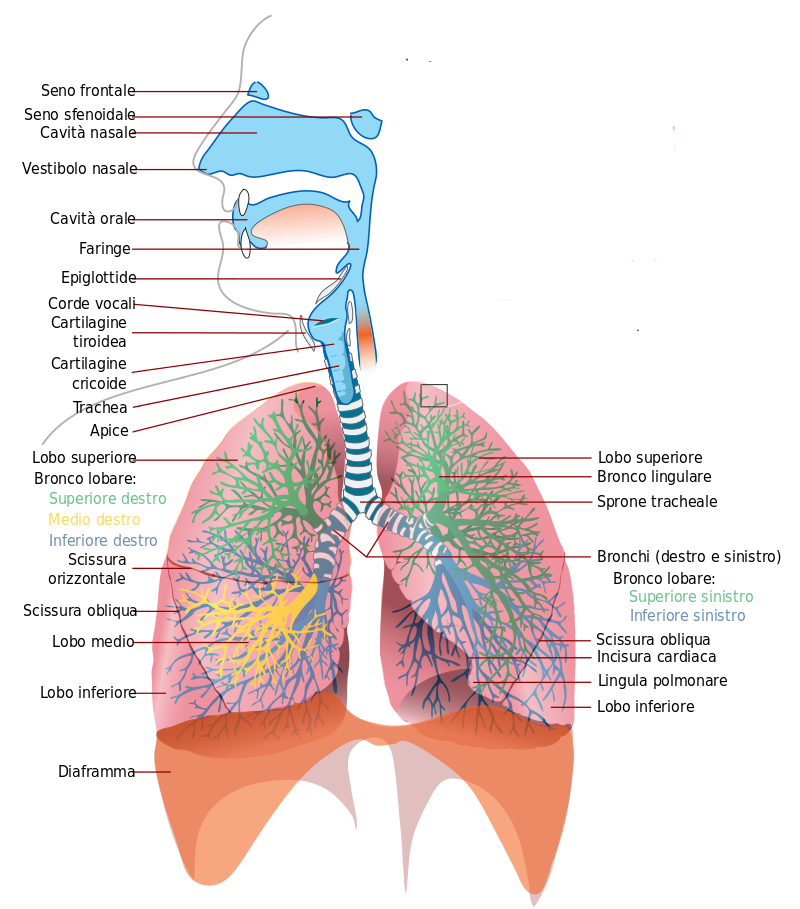
\includegraphics[width=0.6\textwidth]{./Respiratory_system_complete_it.png}
 % appaRespi.jpg: 571x483 pixel, 72dpi, 20.14x17.04 cm, bb=0 0 571 483
  \label{apparatoRespiratorio}
\end{figure}



% \begin{description}
%   \item[Vie aeree.]
\begin{bf}Vie aeree.\end{bf}
    Le vie aeree sono cavit\`a in cui le sostanze gassose, vengono trasportate da o verso i polmoni. Le seguenti parti del corpo sono vie aeree: naso esterno, cavit\`a orale, faringe, laringe, trachea. La figura \ref{apparatoRespiratorio} \cite{appaRespi} \`e una rappresentazione pi\`u esaustiva dell'apparato respiratorio.
%   \item[Polmoni.]


\begin{bf}Polmoni.\end{bf}
    I polmoni sono l'organo essenziale per la respirazione. 
    La loro principale funzione \`e quella di trasportare l'ossigeno dell'ambiente circostante al sangue e di espellere l'anidride carbonica. 
    I polmoni contengono delle piccole sacche d'aria chiamate alveoli. 
    Attraverso i capillari degli alveoli avviene lo scambio per diffusione di ossigeno ed anidride carbonica tra il sangue dell'organismo e l'aria contenuta negli alveoli. 
    Il polmone destro \`e diviso in tre lobi: superiore, medio ed inferiore; mentre quello polmone sinistro \`e diviso in due lobi: uno superiore ed uno inferiore. 
%   \item[Muscoli respiratori.]


\begin{bf}Muscoli respiratori.\end{bf}
    I muscoli respiratori sono il diaframma, i muscoli intercostali, i muscoli addominali, lo sternocleidomastoideo e i muscoli scaleni. Questi muscoli causano l'espansione polmonare.
% \end{description}




\section{Respirazione}

La \emph{respirazione} \`e il processo attraverso il quale l'organismo scambia aria tra i polmoni e l'ambiente circostante. 
La respirazione permette di acquisire ossigeno nel sangue che viene poi usato nel metabolismo e permette di eliminare i residui gassosi del metabolismo come l'anidride carbonica. Durante la respirazione si scambia anche vapore acqueo. 
Il termine usato per indicare il respiro in condizioni normali \`e \emph{eupnea}.  

\subsection{Meccanica della respirazione}

La respirazione \`e ciclica e un ciclo di respirazione ha atto in tre fasi consecutive \cite{meccanicaRespi, wikiMeccaRespi}:
\begin{description}
  \item[Inspirazione.]
    Durante questa fase l'aria viene introdotta nei polmoni. L'inspirazione avviene grazie alla contrazione dei muscoli intercostali e del diaframma, tale contrazione provoca un aumento di volume polmonare e una diminuzione della pressione intrapleurica: ne consegue un'aspirazione dell'aria nei polmoni.
  \item[Espirazione.]
    Durante questa fase l'aria viene espulsa dai polmoni. 
    \`E determinata dal rilascio della forza elastica del parenchima polmonare. Il volume toracico diminuisce, i polmoni vengono compressi e l'aria espulsa.
    \item[Pausa.]
    Tra una espirazione e l'inspirazione successiva ci pu\`o essere una pausa di durata variabile. 
\end{description}

\section{Diagnosi delle malattie dell'apparato respiratorio}



\subsection{Spirometro con pneumotacografo}
Lo spirometro \`e uno strumento utilizzato per misurare i volumi d'aria polmonari. \`E composto da un sensore collegato a un boccaglio, attraverso il quale il paziente respira e da una parte che misura i movimenti di aria provocati dal soggetto. 
Lo spirometro con pneumotacografo \`e un tipo di spirometro dotato di una lamina con la funzione di restringimento e che causa una differenza di pressione. 
Questa differenza pressoria viene misurata da un manometro e poi riconvertita in un segnale proporzionale al flusso generato \cite{WikiSpirPneu, PneumotacofragoTreCani}.

\subsection{Polissonnografia}
La \emph{polisonnografia} \`e una tecnica diagnostica che consiste nella registrazione simultanea di pi\`u parametri fisiologici durante la notte. Normalmente nel corso del test vengono registrati: il flusso d'aria della respirazione, il livello di ossigeno nel sangue, la posizione del corpo, l'attivit\`a cerebrale (attraverso un elettroencefalografo), il movimento degli occhi (attraverso un elettrooculografo) e l'attivit\`a cardiaca (attraverso un elettrocardiografo) \cite{polisonnografo}.

\subsection{Auscultazione}
L'\emph{auscultazione} \`e un sistema di diagnosi che consiste nell'ascoltare i suoni interni del corpo.
Nella accezione che ci interessa, il termine auscultazione ha il significato di ascoltare attraverso uno stetoscopio i suoni prodotti dall'apparato respiratorio. Lo stetoscopio pu\`o essere posizionato in varie parti del torace e della schiena \cite{CARPDWAM}. 

\subsection{Stetoscopio}

Lo stetoscopio
% (dal greco στήθος, stéthos petto, e σκοπή, skopé osservazione) 
\`e uno strumento medico utile all'auscultazione delle parti interne del corpo e sopratutto del torace. Ci sono due tipi principali di stetoscopio:
\paragraph{Stetoscopio acustico.}
    Lo stetoscopio acustico funziona tramite la trasmissione di suoni provenienti dal corpo attraverso dei canali contenenti aria fino alle orecchie dell'ascoltatore.
    Uno dei problemi degli stetoscopi acustici \`e il basso volume del suono trasmesso. 
    Ne consegue una difficolt\`a nell'eseguire una diagnosi precisa.
\paragraph{Stetoscopio elettronico.}
    L'innovazione tecnologica nel campo degli stetoscopi consente oggi la rilevazione di una pi\`u ampia gamma di suoni ed una maggior qualit\`a d'ascolto, con la possibilit\`a di ottenere registrazioni e riproduzioni di grande fedelt\`a dei suoni. 
    A differenza degli stetoscopi acustici, che sono tutti basati sullo stesso metodo di funzionamento, gli stetoscopi elettronici variano molto tra un modello e l'altro. 
    I pi\`u semplici funzionano grazie ad un microfono applicato al petto del paziente, ma di contro, risentono del suono dell'ambiente esterno che spesso causa interferenze. 
    Alcuni stetoscopi elettronici forniscono direttamente un audio in output e si possono usare insieme ad un dispositivo esterno di registrazione. 
    Altri possono trasmettere il segnale via wireless o bluethoot. Un dispositivo (ad esempio un computer) riceve questo segnale e pu\`o fare vari tipi di analisi. 
    Altri modelli, pi\`u complessi, trasformano le onde sonore in impulsi elettrici, cos\`i da poter essere amplificate per un migliore ascolto. 
    Recentemente, alcuni stetoscopi elettronici sono stati dotati di filtri, allo scopo di eliminare le interferenze sonore esterne e in pi\`u sono in grado di poter selezionare il range di frequenza in modo da poter ascoltare separatamente o meno i suoni cardiaci da quelli respiratori. \cite{fusello}


\subsection{Invasivit\`a clinica}

Un parametro molto importante per valutare un sistema diagnostico \`e l'invasivit\`a clinica o semplicemente invasivit\`a. 
Questa si riferisce alla possibilit\`a che l'esame finisca per compromettere ulteriormente lo stato di salute del soggetto. 
Siamo in presenza di un esame invasivo ad esempio, nel caso in cui l'esame possa portare agenti contaminanti (virus, batteri, tossine, sporcizia) all'interno del diretto interessato e quindi causare una infezione che aggravi le condizioni del paziente. 
L'invasivit\`a di un meccanismo diagnostico esce allo scoperto anche nei casi in cui un piccolo errore nella procedura procura danni al paziente \cite{Invasivita}.
Tra i sistemi diagnostici descritti in questa sezione il metodo meno invasivo \`e l'auscultazione.


\section{Patologia dell'apparato respiratorio}

\subsection{Apnee del sonno}
La \emph{sindrome da apnea del sonno} \`e un disordine del sonno caratterizzato da ripetute apnee o ipopnee durante il sonno \cite{ASDBOS}. 
Una \emph{apnea} \`e una pausa di durata anormale nella respirazione che supera i dieci secondi \cite{OSARFSD} e pu\`o durare anche alcuni minuti \cite{NHLBI}. 
Una \emph{ipopnea} \`e un evento caratterizzato da respirazione insufficiente, pi\`u precisamente una ipopnea si verifica quando il flusso d'aria si riduce di almeno il $30\%$ per almeno dieci secondi e la desaturazione di ossigeno nel sangue \`e di almeno il $4\%$ \cite{OSARFSD}. 
Ci sono tre forme di apnea del sonno:
\begin{description}
  \item[Apnea centrale.]
   La respirazione \`e interrotta per via di un mancato movimento dei muscoli respiratori, quindi il volume dei polmoni rimane invariato.
  \item[Apnea ostruttiva.]
    La respirazione \`e interrotta a causa di un blocco fisico nelle vie aeree nonostante persistano movimenti respiratori \cite{AntoniettaBisulli}.
  \item[Apnea mista.]
    La respirazione \`e soggetta a entrambi i tipi di apnea appena descritti.
\end{description}

Le apnee del sonno si verificano sia nei bambini che negli adulti. I soggetti affetti da apnea del sonno possono manifestare i seguenti sintomi: eccessiva sonnolenza durante il giorno, tempi di reazione lenti, problemi alla vista, indebolimento delle funzioni del fegato e altro. 
Inoltre gravi forme di apnee del sonno ostruttive aumentano in modo significativo il rischio di eventi cardiovascolari fatali \cite{OSARFSD, ASAHAIS, SSAAROISITE}.

L'\emph{indice di apnea-ipopnea(apnea-hypopnea index AHI)} \`e definito come il numero di eventi di apnea e di ipopnea in rapporto alla durata del sonno. 
L'AHI \`e un indicatore della gravit\`a della sindrome di apnea del sonno e i suoi valori sono categorizzati tipicamente in: leggera da 5 a 15 episodi all'ora, moderata da 15 a 30 episodi all'ora o severa oltre i 30 episodi all'ora. 

Lo studio \cite{ASDBOS} conclude che c'\`e una forte associazione tra la sindrome da apnea del sonno e l'ictus. 
In particolare dimostra che un indice da moderato a severo di AHI \`e associato ad un alto rischio di ictus e ipotizza che la sindrome da apnea del sonno contribuisca allo sviluppo di un ictus. 
Purtroppo resta ancora da scoprire se esiste un pattern respiratorio specifico che precede immediatamente un ictus.

Lo studio \cite{DNPSDOSA} prende in esame i polisonnogrammi e i certificati di morte di alcune persone che sono decedute a causa di una malattia cardiaca improvvisa. 
Le persone sono state divise in due gruppi: le persone del primo gruppo soffrivano di sindrome da apnea notturna mentre le persone del secondo no. 
Si \`e riscontrato che la maggior parte delle persone appartenenti al primo gruppo sono morte durante il sonno al contrario di quelle del secondo. 
Lo studio conclude che la gravit\`a della sindrome da apnea del sonno \`e direttamente proporzionale al rischio di morte improvvisa per malattie cardiache durante il sonno. 
\\Episodi acuti di apnea o ipopnea possono indurre: ipossiemia, aumento degli impulsi nel sistema nervoso simpatico, aumento brusco nella pressione sanguigna, aumento dello stress delle pareti cardiache, aritmie cardiache, ipercoagulabilit\`a, stress ossidativo vascolare, infiammazioni sistemiche e altro. 
Questo potrebbe spiegare i dati osservati dallo studio. Resta un problema aperto quello di stabilire se nel primo gruppo di persone, la morte \`e immediatamente preceduta da un evento di apnea o ipopnea grave. 


\subsection{Arresto respiratorio}
Un arresto respiratorio \`e l'interruzione della respirazione normale. \`E molto probabile che si verifichino traumi celebrali se l'arresto respiratorio dura pi\`u di tre minuti e la morte \`e quasi certa se questo dura pi\`u di cinque minuti.

\section{Base funzionale dei suoni respiratori}

Secondo \cite{PKW} i suoni normali che si possono sentire sul petto di un soggetto nella fase di inspirazione, vengono generati sopratutto nella parte lobare delle vie respiratorie. I suoni respiratori sono generati da turbolenze dell'aria nelle vie respiratorie. Le caratteristiche dei suoni sono molto variabili, si possono notare differenze da persona a persona che dipendono dal peso, dall'et\`a, dallo stato di salute e altri fattori. I suoni respiratori variano anche rispetto alla densit\`a del gas respirato la quale diminuisce con l'aumentare dell'altitudine rispetto al livello del mare. In generale per\`o l'intensit\`a dei suoni respiratori \`e proporzionale al quadrato del flusso d'aria. 
% mentre nella fase di espirazione questi vengono sopratutto da regioni pi\`u vicine.
Lo studio \cite{DOIAERSINTSOTHT} nota che i suoni inspiratori vengono prodotti in modo predominante nella zone periferiche dei polmoni, mentre i suoni espiratori vengono prodotti nelle zone pi\`u centrali.

\section{Analisi acustica dei suoni respiratori}
\label{sec:Analisiacusticadeisuonirespiratori}

L'articolo \cite{GPA} analizza l'energia spettrale dei suoni respiratori normali ascoltati sul petto di un soggetto. Conclude che questi seguono uno schema caratteristico, in particolare che la potenza decresce in modo esponenziale con la frequenza nell'intervallo dai $75$ ai $2000 Hz$, dopo quest'ultimo valore la potenza \`e trascurabile. Secondo \cite{SKCAKM} il suono registrato sul petto di soggetti sani ha una intensit\`a massima attorno ai $250Hz$ e decresce rapidamente fino ad arrivare ad un livello di intensit\`a trascurabile attorno a una frequenza di circa $1000Hz$. Nel caso dei soggetti malati invece i picchi di frequenze sono pi\`u alti.


Gli articoli \cite{ADT, KoronaKokar, kandaswamy, CACMVS} classificano i suoni respiratori nel modo seguente (riassunto nella figura \ref{classificazioneRespiratori}):
\subparagraph{Suoni respiratori normali}
    I suoni respiratori normali o fisiologici sono i suoni prodotti dal sistema respiratorio di un soggetto sano. 
    Questi suoni sono pi\`u intensi in fase inspiratoria e decrescono in fase espiratoria (nonostante quest'ultima sia pi\`u lunga di quella inspiratoria) e ci\`o \`e dovuto al fatto che l'inspirazione avviene mediante contrazione muscolare, generando un flusso d'aria pi\`u veloce, rispetto all'espirazione, che \`e un fenomeno passivo. 
    I suoni normali hanno un frequenza nell'intervallo dai $100$ ai $1000Hz$. 
    A causa dei suoni prodotti dal movimento dei muscoli del torace e dal diaframma e a causa di quelli prodotti dall'apparato cardiocircolatorio, i suoni dall'apparato respiratorio di solito non vengono studiati a frequenze minori di $60Hz$. 
    I suoni respiratori normali si dividono in:
    \begin{description}
      \item[Murmori vescicolari]
	Si generano per l'azione di filtro degli alveoli sull'aria in arrivo.
      \item[Suoni bronchiali]
	Si generano nelle zone di passaggio dall'albero bronchiale agli alveoli, quindi per mescolanza di rumore bronchiale ed alveolare. 
      \item[Soffio bronchiale]
	Si ascolta in corrispondenza dei grossi bronchi in presenza di addensamento polmonare.
    \end{description}
    
\subparagraph{Suoni respiratori anormali}
    I suoni respiratori anormali o patologici, sono suoni accidentali che non fanno parte del normale ciclo di respirazione. 
    Ci sono due tipi di suoni anormali:
    \begin{description}
      \item[Continui]
	Tra i suoni anormali continui si distinguono: 
	\begin{description}
	  \item[Ronchi o gemiti]
	    Questi suoni sono spesso gravi e sembrano dei rantoli, la loro frequenza dominante \`e $200Hz$, hanno quindi una bassa tonalit\`a. 
	    Sono segno di broncocostrizione e si generano per il passaggio dell'aria in vie aeree ristrette per la presenza di muco o broncospasmo.
	  \item[Rantolo secco (wheezes)]
	    Questi suoni hanno una frequenza dominante attorno ai $100Hz$ e hanno una durata maggiore di $100ms$. 
	    Sono un segnale caratteristico di una malattia ostruttiva polmonare.
	  \item[Sibili]
	    Questi suoni sono dei $wheezes$ molto pi\`u forti e sono la conseguenza di una ostruzione dinamica nella laringe o nella trachea. 
	    L'energia di questi suoni \`e concentrata in massima parte su una frequenza che si aggira attorno ai $1000Hz$.
	\end{description}
      \item[Discontinui]
	Tra i suoni anormali discontinui si notano:
	\begin{description}
	  \item[Rantolo (Crackles)]
	    Questi suoni hanno una durata minore di $10ms$ e cadono in un vasto spettro di frequenze, tra $200$ e $2000Hz$. Di solito sono indice di malattie cardiorespiratorie.
	  \item[Fine  crackles]
	    Sono i rantoli fini, anche detti rantoli crepitanti e hanno una tonalit\`a alta. Sono dovuti alla ritardata apertura degli alveoli. Talvolta ad essi si sovrappongono gli sfregamenti pleurici, il cui reperto \`e molto simile.
	  \item[Coarse crackles]
	    Sono i rantoli subcrepitanti, di una tonalit\`a bassa, il cui reperto si modifica con la tosse. Sono segno di bronchite e si generano per il passaggio dell'aria attraverso il muco.
	  \item[Squawks]
	    Questi suoni sono dei sibili di breve durata.
	\end{description}
    \end{description}


% 
% \begin{table} [h]
%   \begin{tabular}{l l l l}
%     Suono			& Durata 		& Spettro   		  	& Tipo\\
%     \hline\\	
%     suoni normali bronchiali   & -	 		& da $100Hz$ a $1000Hz$		& normale continuo\\
%     suoni normali vescicolari  & -			& da $100Hz$ a $1000Hz$		& normale continuo\\
%     ronchi			& -			& $\sim 200Hz$			& anormale continuo\\
%     wheeze	 		&da $100ms$ a $250ms$	& $\sim 100Hz$			& anormale continuo\\
%     stridor			&-			& $\sim 1000Hz$			& anormale continuo\\
%     crackles			&$<10ms$		&da $200$ a $2000Hz$		& anormale discontinuo\\
%     squawks 			&			&				& anormalediscontinuo\\
%     \hline\\
%   \end{tabular}
% \caption{Classificazione dei suoni respiratori}
% \label{ClassificazioneSuoniRespiratori}
% \end{table}



\begin{center}
\begin{figure}
 

\begin{tikzpicture}
%   [scale=.8,auto=left,every node/.style={fill=blue!20}]
[->,>=stealth',shorten >=1pt,auto,node distance=3cm,
  thick,main node/.style={circle,fill=blue!20,draw,font=\sffamily\Large\bfseries}]
  \node (respiri) at 	(0,3) {suoni respiratori};

  \node (normali) at 	(3,2) {normali};
  \node (anormali) at 	(3,4) {anormali};

  \node (vescicolari) at 	(7,2) {vescicolari};
  \node (bronchiali) at 	(7,1) {bronchiali};
  \node (soffi) at 		(7,1.5) {soffi};

  \node (continui) at 		(7,3) {continui};
  \node (discontinui) at 	(7,5) {discontinui};

  \node (ronchi) at 		(11,2.5) {ronchi};
  \node (rantoli) at 		(11,3) {rantoli};
  \node (sibili) at 		(11,3.5) {sibili};

  \node (fine) at 		(11,4.5) {fine crackles};
  \node (squawks) at 		(11,5) {squawks};
  \node (coarse) at 		(11,5.5) {coarse crackles};  


   \foreach \from/\to in {respiri/normali,respiri/anormali,
    normali/vescicolari,normali/bronchiali,normali/soffi, 
    anormali/continui, anormali/discontinui,
    continui/ronchi,continui/rantoli,continui/sibili,
    discontinui/coarse, discontinui/fine, discontinui/squawks}
     \draw (\from) -- (\to);

\end{tikzpicture}
\caption{Classificazione dei suoni respiratori}
\label{classificazioneRespiratori}
\end{figure}
\end{center}



I risultati ottenuti da \cite{DOIAERSINTSOTHT} ci dicono che in media, i suoni inspiratori hanno una intensit\`a di circa $10db$ maggiore rispetto ai suoni espiratori a parit\`a di flusso. 
Inoltre i suoni registrati da microfoni in prossimit\`a della trachea sono pi\`u intensi di quelli registrati da microfoni sul petto.

I rantoli di solito vengono registrati in prossimit\`a della trachea, dove gli effetti del filtraggio del corpo sono minimi. 
D'altro canto, i suoni discontinui accidentali generati a causa di patologie polmonari vengono riconosciuti meglio sulla parte basale bassa dei polmoni \cite{TLSA}.

\paragraph{Rumore} 
Ci sono altri suoni fisiologici che complicano l'auscultazione dei suoni respiratori. 
Se l'auscultazione avviene sul torace, questi sono i suoni cardiovascolari e i suoni gastrointestinali. 
Se si auscultano i suoni tracheali allora la fonte di disturbo sono i suoni dovuti alla deglutizione della saliva.

\section{Schemi di respirazione}
\label{schemirespiri}

Lo studio \cite{BP} analizza gli schemi o pattern di respirazione normali. I soggetti coinvolti nello studio sono $65$ e hanno et\`a dai $20$ agli $81$ anni. Vari parametri sono stati presi in considerazione tra i quali: la frequenza di respirazione e il tempo di inspirazione. Lo studio conclude che la media delle frequenze di respirazione \`e $16.6\pm 2.8$ respiri al minuto mentre la durata media dei tempi di inspirazione \`e di $1.62\pm 0.31$ secondi.
Una frequenza di respirazione media di $16.6$ respiri al minuto implica una durata media di $3.6s$ a respiro.
Esistono vari schemi di respirazione anormali alcuni dei quali sono elencati nella figura \ref{respirazioneAnormali}. 
Descriviamo pi\`u in dettaglio gli schemi che compaiono nella figura dall'alto verso il basso:
  \begin{wrapfigure}{r}{0.5\textwidth}
     \begin{center}
  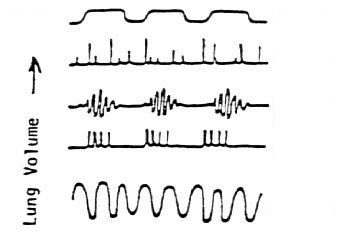
\includegraphics[width=0.48\textwidth]{./abnormalBreathingPatterns.jpg}
     \end{center}
    \caption{Elenco di pattern respiratori \cite{ABP}}
    \label{respirazioneAnormali}
\end{wrapfigure}



\paragraph{Apneosi.}
L'apneosi \`e uno schema di respirazione caratterizzato da profondi annaspamenti durante l'inspirazione, dopo una inspirazione avviene una lunga pausa seguita da un rilascio insufficiente di aria.
Notiamo che durante l'apneosi la pausa avviene dopo l'inspirazione e non dopo l'espirazione come nella sindrome da apnea ostruttiva.

\paragraph{Respiro agonico.}
Il respiro agonico \`e uno schema anormale di respirazione caratterizzato da boccheggiamento e da una riduzione estrema della frequenza degli atti respiratori fino al loro totale arresto. 
L'uso corretto del termine si deve restringere all'ultimo respiro prima della morte. 

\paragraph{Respiro di Cheyne Stokes.}
Il respiro di Cheyne Stokes \`e uno schema di respirazione anormale nel quale il respiro si fa da prima progressivamente pi\`u frequente e profondo, poi la frequenza respiratoria diminuisce gradualmente fino a portare ad una apnea. 
Lo schema si ripete e ogni ciclo di solito dura dai $30$ secondi ai $2$ minuti. 

\paragraph{Respiro di Kussmaul.}
Il respiro di Kussmaul \`e una forma di iperventilazione compensatoria. 
\`E caratterizzato da atti respiratosi molto lenti ed in particolare da una inspirazione profonda e rumorosa a cui segue una breve apnea, poi una espirazione breve e gemente e infine una pausa post-espiratoria decisamente prolungata.





\chapter{Acustica e audio digitale}

\section{L' acustica e il suono}

L'acustica \`e quella branca della fisica che studia il suono, le sue cause, la sua propagazione e la sua ricezione.
La percezione sonora \`e normalmente legata alle vibrazioni del timpano nell'orecchio. 
Queste vibrazioni sono provocate da piccole variazioni di pressione nell'aria. 
La variazione di pressione dell'aria \`e quindi l'equivalente fisico del suono \cite{EAP}.
La vibrazione provoca una successione di compressioni e rarefazioni nel mezzo dell'ambiente circostante e tale disturbo comincia a propagarsi lontano dalla sorgente in tutte le direzioni (un caso visibile \`e quello delle onde sull'acqua). 
L'effetto uditivo, consiste nella percezione da parte di un apposito dispositivo (orecchio di esseri viventi o microfoni artificiali) delle piccole e rapidissime vibrazioni emesse appunto da una "sorgente sonora".

\section{Onde sonore}
La natura fisica del suono \`e di tipo ondulatorio, ovvero descrive un movimento che pu\`o essere rappresentato tramite un onda. 
Si tratta di onde meccaniche che trasportano energia lontano dalla sorgente sonora.
Alcune principali grandezze delle onde sono \cite{SELET}:
   \begin{description}
      \item[Periodo.] 
	Il periodo, o durata dell'oscillazione rappresenta il tempo in cui l'onda compie un'oscillazione e torna alla condizione iniziale.  
      \item[Frequenza.]
	La frequenza di un onda indica il numero di cicli completi che compie in un secondo:
	\[
	  f = \frac{1}{t}
	\]
	dove $f$ \`e la frequenza e $t$ \`e il periodo.
	In generale la frequenza di un evento si misura in $Hz$. 
	Ricordiamo che un $Hz$ \`e il numero di eventi che accadono in un secondo. 
      \item[Ampiezza.]
      L'ampiezza o intensit\`a invece \`e il valore massimo raggiunto dall'oscillazione stessa durante un periodo ed \`e determinata dalla quantit\`a di energia impiegata. 
      Viene espressa tramite i decibel.
      \item[Forma.]
	La forma dell'oscillazione \`e determinata dal numero delle componenti parziali e dal loro rapporto di frequenza, ampiezza e  fase. 
	Essa rappresenta l'aspetto dell'onda in base all'ampiezza e al tempo servendosi di coordinate cartesiane. 
    \end{description}
    
\begin{figure}[h!]
 \centering
 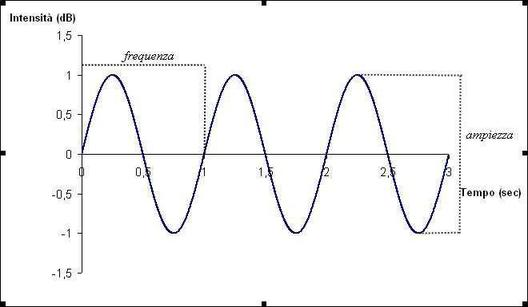
\includegraphics[width=0.5\textwidth]{./OndaSonora.jpg}
 % envelope.png: 220x138 pixel, 96dpi, 5.82x3.65 cm, bb=0 0 165 104
  \label{OndaSonora}
\caption{Rappresentazione delle principali grandezze dell'onda sonora \cite{IONDASON}}
\end{figure}



\section{Suono analogico e digitale}

Il suono \`e un flusso informativo di natura temporale che scorre all'interno di apparecchiature elettroniche. 
Questa informazione pu\`o essere rappresentata in due forme: analogico e digitale. 
Una rappresentazione analogica \`e una rappresentazione o trasformazione di una grandezza fisica tramite una sua analogia: in altre parole, si intende un sistema in cui una quantit\`a fisica continuamente variabile viene rappresentata da un'altra (ad esempio, la tensione di un segnale elettrico) nel modo pi\`u fedele possibile. 
La curva continua nel tempo delle variazioni di ampiezza viene rappresentata da una curva continua nel tempo delle variazioni di tensione elettrica. 


Una rappresentazione digitale non cerca di imitare la curva continua di ampiezza con una curva analoga ad essa, ma piuttosto assegna dei numeri che rappresentano di volta in volta il valore dell'ampiezza in istanti successivi di tempo. 
Sar\`a la successione di numeri a rappresentare l'andamento della curva. 
La rappresentazione digitale non \`e continua, ma discreta; cio\`e esistono degli eventi ben definiti che sono i valori dell'ampiezza in precisi istanti di tempo. 
I vantaggi della rappresentazione digitale e cio\`e di un codice simbolico sono molti: dalle operazioni di copia del segnale, a quelle di manipolazione. 
Ma un aspetto totalmente nuovo \`e la possibilit\`a di correzione degli errori introdotti dai supporti per la memorizzazione. 
Per errore si intende che alcuni numeri che rappresentano il segnale vengono letti in maniera differente da come era stati memorizzati o trasmessi.

\subsection{Discretizzazione}
Per sottoporre un segnale analogico ad elaborazioni digitali \`e necessario prima convertirlo in una sequenza di dati binari, ottenuti tramite due operazioni di discretizzazione: una discretizzazione nel dominio del tempo o campionamento che riduce gli infiniti valori di un segnale analogico in sequenze di campioni discreti e una discretizzazione nel dominio delle ampiezze o quantizzazione (del livello) che permette di rappresentare ciascun campione con un numero finito di bit. 
La necessit\`a di elaborare il segnale in forma digitale porta a limitare il numero delle informazioni e quindi a misurare le grandezze solo a valori discreti del tempo, attribuendo loro un certo numero discreto di valori, variabili fra un massimo e un minimo. 
I segnali acquisiti diventano quindi serie di valori corrispondenti agli istanti per cui si \`e effettuato il campionamento.

\begin{figure}[h!]
 \centering
 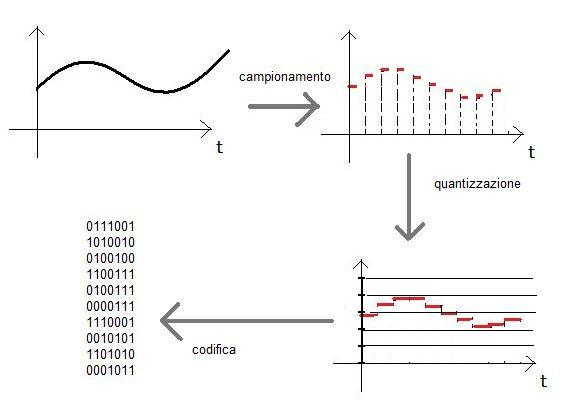
\includegraphics[width=0.5\textwidth]{./AnalogicoDigitale.jpg}
 % envelope.png: 220x138 pixel, 96dpi, 5.82x3.65 cm, bb=0 0 165 104
  \label{AnalogicoDigitale}
\caption{Discretizzazione di un suono da analogico a digitale}
\end{figure}

 
\subsubsection{Campionamento} 
Campionare l'audio significa creare una sequenza di campioni, ovvero i valori di un segnale audio in diversi momenti temporali quindi ogni campione memorizzato rappresenta un'ampiezza ad un dato istante. 
Viene chiamata frequenza di campionamento il numero di volte che viene campionato il segnale in un secondo.  \cite{elabA}.


Secondo il teorema di campionamento di Nyquist e Shannon in una conversione da analogico a digitale la minima frequenza di campionamento necessaria per evitare ambiguit\`a e perdita di informazione nella ricostruzione del segnale analogico originario, con larghezza di banda finita e nota, \`e pari al doppio della frequenza massima del suono che stiano convertendo.
Se non viene rispettato questo teorema, cio\`e si ha un sottocampionamento del segnale analogico nel dominio del tempo allora nel dominio delle frequenze si ha la produzione di frequenze non proprie del segnale originario (\textit{alias}) producendo cio\`e una distorsione del segnale originario divenuto ora non pi\`u fedele.

\begin{figure}[h]
 \centering
 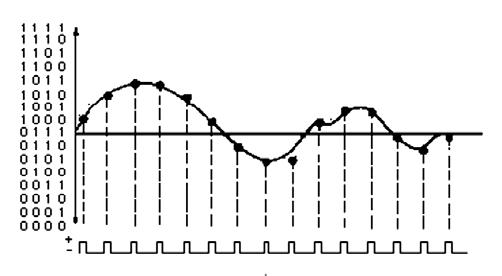
\includegraphics[width=0.7\textwidth]{./campionamento.jpg}
 % envelope.png: 220x138 pixel, 96dpi, 5.82x3.65 cm, bb=0 0 165 104
  \label{campionamento}
\caption{Campionamento e quantizzazione di un segnale continuo.}
\end{figure}


% Il segnale viene campionato e convertito in una sequenza di numeri, che vengono
% codificati con simboli. In generale, i segnali appartengono al mondo fisico e sono dovuti a fenomeni di
% tipo diverso. Ad esempio, il suono \`e dovuto alle variazioni della pressione dell’aria.
% Un sensore traduce la grandezza fisica in un segnale elettrico, che viene
% campionato e convertito in formato digitale.
% Al termine del processo di conversione, il segnale \`e stato trasformato in una
% sequenza di numeri che pu\`o essere elaborata, memorizzata o trasmessa.
% Il processo inverso consiste nel convertire i numeri in una sequenza di impulsi
% elettrici, che viene filtrata in modo da renderla simile al segnale originale. Il
% segnale elettrico cos\`i ottenuto viene inviato ad un trasduttore, che lo converte in
% un segnale fisico (suono).

\subsubsection{Quantizzazione}

Dopo il campionamento, la conversione analogico-digitale viene completata con la quantizzazione, che consiste nell'associare ad ogni campione un valore discreto.


Per ottenere ci\`o i valori possibili della grandezza in questione vengono innanzitutto limitati tra un massimo ed un minimo intorno a dei valori discreti preventivamente definiti, definendo cos\`i le relative regioni di decisione e la dinamica del quantizzatore stesso: in tal modo il valore analogico della grandezza originaria, 
in corrispondenza del valore campionato in ascissa, verr\`a ricondotto al pi\`u prossimo dei valori discreti preventivamente definiti tramite il processo di decisione.


Con la quantizzazione vengono per\`o introdotti degli errori detti \textit{errori di quantizzazione} pari alla differenza tra il valore quantizzato e il suo valore "reale" nel campo continuo. 
L'errore massimo possibile che potr\`a essere introdotto volta per volta sar\`a quindi pari alla met\`a dell'intervallo discreto discriminabile o regione di decisione. L'insieme di questi errori conduce al rumore di quantizzazione.


\section{Segnale}
In generale un segnale \`e una funzione di una o pi\`u variabili che contiene informazioni relative ad un fenomeno fisico. In questo caso ci interessano i segnali sonori che sono delle funzioni dell'ampiezza rispetto al tempo. 
I segnali possono essere classificati secondo le seguenti propriet\`a:
\begin{description}
  \item[Continuit\`a nel tempo]
    Un segnale pu\`o essere a tempo continuo o a tempo discreto a seconda che il dominio della funzione sia non numerabile o numerabile.
  \item[Continuit\`a nell'ampiezza]
    Un segnale pu\`o essere ad ampiezza continua oppure ad ampiezza discreta(o quantizzato) a seconda che l'immagine della funzione sia non numerabile o numerabile.
  \item[Periodicit\`a]
    Un segnale pu\`o essere periodico se esiste una quantit\`a $T$ nel dominio del tempo tale che per ogni tempo $t$ vale $s(T+t)=s(t)$. Se non vale questa propriet\`a allora il segnale \`e aperiodico. 
    Un segnale si dice quasi periodico se \`e composto dalla somma di segnali periodici con diverse frequenze che tra di loro stanno in rapporti non razionali. 
  \item[Determinatezza]
    Un segnale si dice determinato se \`e perfettamente noto e rappresentabile con una funzione che ne specifica l'andamento in ogni istante invece viene chiamato aleatorio se non \`e completamente noto a priori, ma pu\`o assumere un qualunque andamento entro una classe di funzioni specificata da alcune propriet\`a statistiche.
  \item[Stazionareit\`a]
    Un segnale stocastico, si dice stazionario se le sue propriet\`a statistiche non cambiano nel tempo, altrimenti si dice non stazionario.
\end{description}



\paragraph{Energia}
Dato un segnale $s(t)$ definiamo l'energia del segnale come:
\[
  E=\int_{-\infty}^{\infty} |s(t)|^{2}dt
\]
La definizione acquista significato fisico quando il segnale \`e reale, in tal caso, infatti supponendo che $s(t)$ rappresenti la tensione applicata o la corrente immessa ad una resistenza di $1Ohm$, questa \`e l'energia da essa dissipata. 
Definiamo la potenza media di un segnale continuo $s(t)$ il limite:
\[
  P=\frac{1}{2T} \lim_{T\rightarrow \infty} \int_{-T}^{T} |s(t)|^{2}dt
\]

Il segnale $s(t)$ \`e detto ad energia finita se $E$ \`e finito e diverso da zero. 
Il segnale \`e detto a potenza media finita se P \`e finito e diverso da zero. Si noti che se un segnale ha energia finita la sua potenza media \`e nulla e se un segnale ha potenza media finita la sua energia \`e infinita, pertanto le due classi sono disgiunte. 
Una classe importante di segnali a potenza media finita \`e costituita dai segnali periodici; in tal caso l'energia \`e finita e la potenza media coincide con quella calcolata in un periodo.



\section{Analisi nel dominio del tempo e nel dominio della frequenza}
\begin{comment}
dato un segnale infinito il suo contenuto in frequenza (il suo spettro) si pu\`o ottenere con una operazione matematica detta Integrale di Fourier. Il risultato dell'Integrale di Fourier di s(t) \`e una funzione a valori complessi S(ω) definita tra meno infinito e pi\`u infinito. I valori complessi portano con sé l'informazione relativa alla fase del segnale. 
Per esempio se si considera il segnale emesso da un sistema di altoparlanti multivia, spostando la posizione del tweeter cambia la fase del segnale e non il suo contenuto in frequenza, in altri termini il valore assoluto dell'Integrale di Fourier resta lo stesso. 
L'integrale di Fourier \`e reversibile, nel senso che a partire dal contenuto in frequenza si pu\`o costruire esattamente il segnale originale. 
Ricordo che stiamo parlando di operazioni matematiche svolte su segnali infiniti lavorando con quantit\`a senza errori, in altra parola segni di lapis su di un pezzo di carta ed esattamente va inteso in questo senso. 
Di solito quando si parla di spettro di un segnale si trascura la fase e si considera |S(ω)| (oppure se ci interessa la potenza espressa in decibel la quantit\`a 20 Log10 | S(ω)|). 
In entrambi i casi si pu\`o dimostrare che la parte positiva e la parte negativa delle funzioni risultanti sono specularmente uguali e quindi di solito se ne disegna solo la parte positiva. 
Con questa semplificazione per\`o si perde la reversibilit\`a e quello che resta \`e solo una misura effettuata sul segnale, priva dell'informazione completa. Per comprendere appiano il significato dell'integrale di Fourier sono necessari alcuni preliminari matematici.
\end{comment}
I principali metodi di analisi del segnale possono essere riassunti nei concetti di analisi nel dominio del tempo e analisi nel dominio della frequenza. 
\`E importante osservare che questi due modi di affrontare un problema sono tra loro intercambiabili, nel senso che, sotto opportune condizioni, nessuna informazione viene persa nel passare da un dominio all'altro. 
Il vantaggio che deriva dall'introduzione dei due domini \`e la possibilit\`a di cambiare la prospettiva con la quale si osserva un dato fenomeno. 
In questo modo un problema che appare di difficile soluzione in un dominio pu\`o risultare molto pi\`u semplice nell'altro \cite{DomTF}.

\paragraph{Analisi nel dominio del tempo}
Questa forma di rappresentazione \`e quella che ci \`e maggiormente familiare, in essa appaiono le variazioni subite dal segnale al trascorrere del tempo. 
Lo strumento pi\`u frequentemente usato e che opera notoriamente nel dominio del tempo \`e l'oscilloscopio.

\paragraph{Analisi nel dominio della frequenza}

Invece di analizzare le variazioni del segnale al passare del tempo, mostra come e quanto un segnale si suddivide o \`e distribuito nelle varie bande di frequenza, definite all'interno di un dato range. 
Viene chiamata analisi spettrale e lo strumento matematico che consente di trasferire lo studio dei segnali e dei sistemi dal dominio del tempo al dominio della frequenza \`e la trasformata di Fourier.

%
\begin{figure}[htbp]
\centering
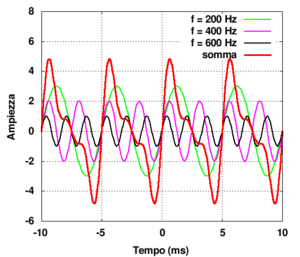
\includegraphics[width=0.4\textwidth]{./DominioTempo.png}%
\qquad\qquad
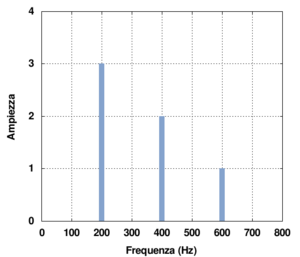
\includegraphics[width=0.4\textwidth]{./DominioFrequenze.png}
\caption{Esempi di grafici nel dominio del tempo e nel dominio delle frequenze \cite{IDOMTF}}
\end{figure}
\section{Analisi armonica e trasformata di Fourier}

L'analisi armonica \`e la branca della matematica che studia la rappresentazione delle funzioni o dei segnali come sovrapposizione di onde fondamentali. 
Indaga e generalizza la nozione di serie di Fourier e trasformata di Fourier. 


\begin{comment}
Data una funzione $s(t)$ reale o complessa a quadrato sommabile, periodica di periodo $2\pi$, per ogni $n$ intero esistono i coefficienti complessi:
\[
c_{n} = \frac{1}{2\pi} \int_{0}^{2\pi}e^{i\cdot n\cdot t}s(t)dt
\]
e la funzione pu\`o essere rappresentata come
\[
s(t) = \sum_{n=-\infty}^{\infty} c_{n} e^{i\cdot n\cdot t}
\]
\end{comment}

L'interpretazione dello sviluppo in serie di Fourier \`e che un segnale periodico di potenza finita si pu\`o sviluppare come combinazione lineare di funzioni periodiche semplici la cui frequenza \`e un numero intero. 
Il tutto si generalizza facilmente al caso in cui il periodo sia $T$ e quindi la frequenza fondamentale abbia il valore $1/T$. 

L'importanza della formula \`e che tutta l'informazione di una funzione periodica continua pu\`o essere espressa con un infinit\`a numerabile (quindi discreta) di valori complessi.


\subsection{Serie di Fourier}

La serie di Fourier \`e una rappresentazione di una funzione mediante una combinazione lineare di funzioni sinusoidali fondamentali.
Un segnale $f(t)$ e' una funzione e quindi si pu\`o decomporre usando una serie di Fourier. La decomposizione di un segnale attraverso una serie di Fourier ci da una descrizione delle frequenze che lo compongono \cite{fourier, fourier3}.

Sia $f(x)$ una funzione definita sui numeri reali e periodica di periodo $2\pi$. Diremo che $f(x)$ \`e sviluppabile in serie di Fourier se esistono dei coefficienti $a_{0}, a_{k}, b_{k}$ con $k$ numero natuale tali che
\[
  f(x) = a_{0} + \sum_{k\in \mathbb{N}} (a_{k} cos(kx) + b_{k} sen(kx))
\]
La formula precedente \`e lo sviluppo in serie di Fourier della funzione $f$ e i coefficienti di Fourier si possono calcolare nel seguente modo:
\[
  \begin{array}{lll}
      a_{0}=\frac{1}{2 \pi} \int_{-\pi}^{\pi} f(x) dx
    &
      a_{k}=\frac{1}{\pi} \int_{-\pi}^{\pi} f(x) cos(kx) dx
    &
      b_{k}=\frac{1}{\pi} \int_{-\pi}^{\pi} f(x) sen(kx) dx
  \end{array}
\]

\cite{fourier2}

\subsection{Trasformata di Fourier}

La trasformata di Fourier permette di scomporre e successivamente ricombinare, un segnale generico in una somma infinita di sinusoidi con frequenze, ampiezze e fasi diverse. L'insieme di valori in funzione della frequenza \`e detto spettro di ampiezza e spettro di fase. 

Se il segnale in oggetto \`e un segnale periodico, la sua trasformata di Fourier \`e un insieme di valori discreti, che in tal caso prende il nome di spettro discreto o spettro a pettine. 
Mentre nel caso in cui il segnale sia non periodico lo spettro \`e continuo, e tanto pi\`u \`e esteso lungo l'asse delle frequenze quanto pi\`u \`e limitato nel dominio originario della variabile indipendente, e viceversa.
Se il segnale ha un valore medio diverso da zero la serie restituisce anche una componente costante che lo rappresenta.

Sia $f\in L^{1}(\mathbb{R}^{n})$ una funzione integrabile, la trasformata continua di Fourier, detta anche semplicemente trasformata di Fourier, e' definita nel modo seguente:
\[
  \mathbb{F}(f)=  t\mapsto \frac{1}{(2\pi)^{\frac{n}{2}}} \int_{\mathbb{R}^{n}} e ^{-i\cdot t \cdot x} dx
\]

\cite{fourier}\cite{fourier3}

\subsection{Trasformata discreta di Fourier}

La trasformata di Fourier opera su funzioni continue, sia nel dominio dei tempi che delle frequenze. Al contrario, la trasformata discreta di Fourier opera su funzioni a dominio discreto. Sia $S_{n}$ un insieme di sequenze periodiche di periodo $n$. Un generico elemento di $S_{n}$ si puo' scrivere come $y=\{y_{j}\}_{j\in \mathbb{N}}$ e si puo' pensare come un segnale periodico discreto nel quale $y_{j}$ e' il valore del segnale al tempo $j$. Definiamo la trasformata discreta di Fourier di $y$ come la sequenza
\[
  (\mathbb{F}_{n}(y))_{k} = z_{k}
\]
dove
\[
  \begin{array}{lll}
      z_{k}=\displaystyle\sum_{j=0}^{n-1} y_{j} \overline{w}^{j \cdot k}
    &
    &
      w=\exp\left(\displaystyle\frac{s \pi i}{n}\right)
  \end{array}
\]
 
\cite{fourier}
\section{Wavelet}

 \begin{comment}
Il processo di convertire un segnale dal dominio del tempo a dom delle frequenze viene fatto tramite la trasformatadi Fourier (FT). Però Fourier non fornisce informazioni sufficienti su segnali non stazionari. FT determina soltanto le componenti di frequenza di un segnale, ma non la loro posizione nel tempo. Per risolvere questo inconveniente di usa STFT che usa una tecnica di “finestraggio”.
STFT associa il segnale in uno spazio bidimensionale di tempo e di frequenza utilizzando una singola finestra fissa.
Trasformata wavelet consente l'analisi con durate finestre multiple che consentono una prospettiva grossolana a multirisoluzione fine del segnale.
Essere in grado di dilatare o comprimere la regione variabile della finestra di dimensioni (wavelet), diverse caratteristiche del segnale saranno estratte in WT.
\end{comment}
Il processo di convertire un segnale dal dominio del tempo a dominio delle frequenze viene fatto tramite la trasformata di Fourier, per\`o Fourier non fornisce informazioni sufficienti su segnali non stazionari in quanto determina soltanto le componenti di frequenza di un segnale, ma non la loro posizione nel tempo.
La trasformata Wavelet consente un' analisi migliore per questo tipo di segnali. 

Una wavelet \`e una forma d'onda oscillante di lunghezza finita, con un ampiezza che parte da zero e aumenta e decrementa tornando a zero.
Al contrario delle sinusoidi usate nella trasformata di Fourier, le wavelet sono pi\`u concentrate nel tempo. 
Di solito forniscono una anailsi del segnale che \`e localizzato sia nel tempo che nella frequenza mentre la trasformata di Fourier \`e localizzata solo nella frequenza. 
Un esempio di wavelet \`e rappresentato dalla figura seguente:
\begin{comment}
\begin{figure}[h]
 \centering
 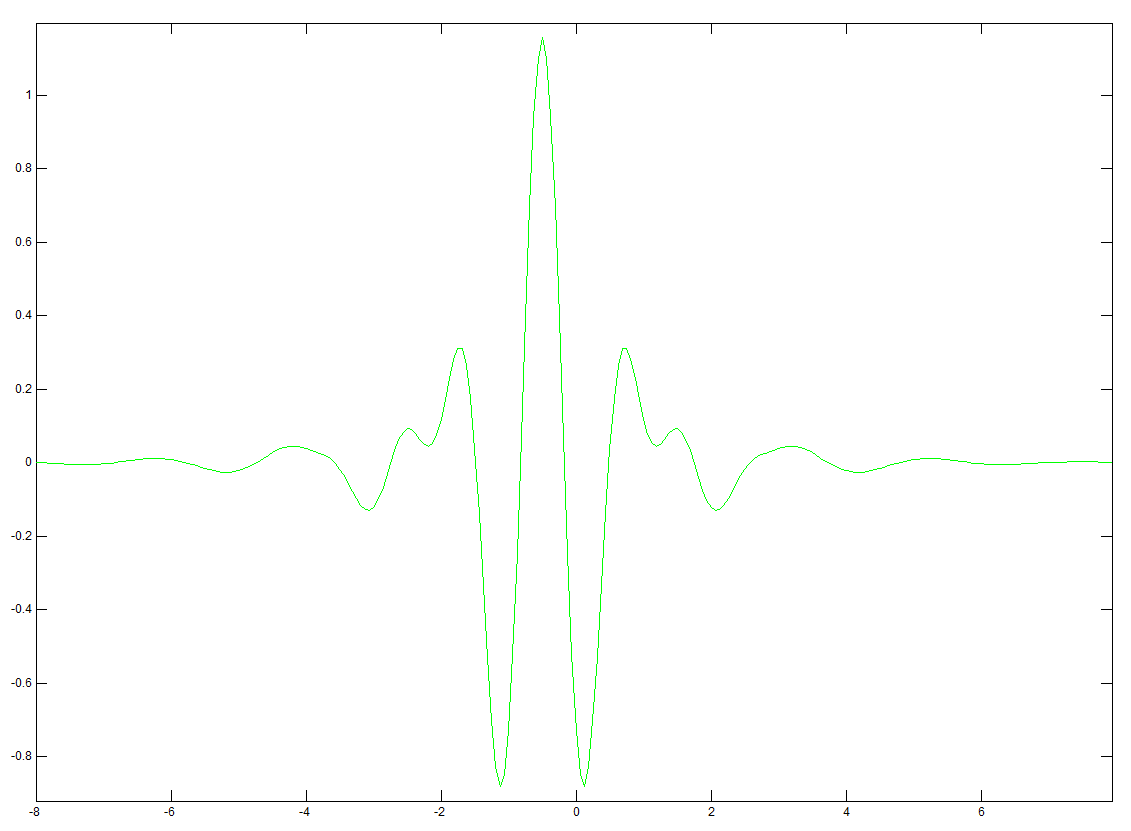
\includegraphics[width=0.4\textwidth]{./Meyerwavelet.png}
 % Meyerwavelet.png: 1131x831 pixel, 72dpi, 39.90x29.32 cm, bb=0 0 1131 831
 \label{fig: Meyer wavelet}
\end{figure}
\end{comment}


Una funzione $\psi(t)$ \`e una wavelet se soddisfa i seguenti criteri:
\begin{itemize}
  \item 
    Una wavelet deve avere energia finita.
    \[
      E=\displaystyle \int_{-\infty}^{\infty} |\psi(t)|^{2} dt < \infty
    \]
  \item
    Se $\Psi$ \`e la trasformata di Fourier della wavelet $\psi(t)$ allora $\Psi(0)=0$. Cio\`e la wavelet non ha componenti nella frequenza zero.
  \item
    La trasformata di Fourier di una wavelet complessa deve essere reale e deve essere nulla nelle frequenze negative.
\end{itemize}

\section{Trasformata wavelet continua}
Sia $\psi(t)$ una wavelet, definiamo la trasformata wavelet continua di una funzione $x(t)$ come 
\[
  X(a,b)=\displaystyle \frac{1}{\sqrt{a}}\displaystyle\int_{-\infty}^{\infty} \psi \left( \frac{t-b}{a} \right) x(t) dt
\]

La scala o parametro di dilatazione $a$ corrisponde all'informazione di frequenza e il parametro di traslazione $b$ si riferisce alla locazione della funzione wavelet mentre viene fatta spostare lungo il segnale quindi corrisponde all'informazione temporale nella trasformata.
%Ci sono molte scelte per la wavelet madre.
Esiste anche la trasformata wavelet discreta che opera su segnali a tempo discreto e che restituisce coefficienti discreti nel dominio delle wavelet.
I parametri $a$ e $b$ assumono valori in una griglia discreta
\[
  \begin{array}{llll}
      a=2^{-j}
    &
      b=k\cdot 2^{-j}
    &
     
    &
      j,k\in \mathbb{Z}
  \end{array}
\]


\cite{wavelet1}\cite{wavelet2}

%modificato in tesi.tex--> aggiunto \usepackage{verbatim}
\chapter{Filtri digitali}


\section{Denoising}

Uno degli ostacoli principali dell'analisi computerizzata dei suoni polmonari \`e la presenza di rumore nei segnali. 
In questo caso per rumore si intendono quei suoni provenienti da strumenti come ventilatore, aria condizionata, e altri rumori ambientali che possono contaminare i segnali sonori del polmone. 
La natura rumorosa dei suoni polmonari \`e un fattore di impedimento che vieta l'identificazione di funzioni utili per la diagnostica. 
Quindi il denoising di segnali sonori polmonari \`e d'obbligo per l'utilizzo efficace della diagnosi e in questo capitolo approfondiremo le varie tecniche per l'eliminazione dei rumori.

\section{Classificazione dei filtri digitali}

Un filtro digitale \`e una funzione in grado di modificare il contenuto armonico di un segnale elettrico complesso.
Queste modifiche si esprimono in termini di fasci di frequenze che vengono evidenziate o soppresse a seconda delle caratteristiche del tipo di filtro usato.
Una importante penalizzazione per i filtri digitali \`e che sono limitati nelle frequenze: un filtro digitale deve sempre e comunque rispettare il teorema di Nyquist, ovvero il teorema del campionamento, che impone al filtro un limite massimo sulle frequenze che pu\`o elaborare, altrimenti si ottengono segnali disturbati da aliasing.

Si distinguono due classi di filtri: lineari e non lineari.
\begin{description}
      \item[Filtri lineari]
	  La funzione d\`a in uscita un valore che \`e una combinazione lineare dei valori compresi nella finestra del segnale appena analizzato, cio\`e l'output del filtro pu\`o mettersi in relazione con i valori presi in ingresso. Si possono definire filtri lineari che puliscono il segnale dal rumore oppure che esaltano le discontinuit\`a.
      \item[Filtri non lineari]
	  Per questo tipo di filtro non \`e possibile definire un operatore lineare; solitamente sono operatori di rango, cio\`e operatori che agiscono sui valori presi in ingresso dopo averli ordinati quindi l'output dipende contemporaneamente da pi\`u ingressi.
 \end{description}
La differenza sostanziale tra i due tipi di filtri \`e che, mentre per i primi si pu\`o applicare la trasformata di Fourier con tutte le sue propriet\`a, nei secondi questa operazione non \`e possibile.

\subsection{Categorie di filtri}

I filtri si dividono in quattro principali categorie:

\subsubsection{Filtro passa alto}

Il filtro passa alto permette il passaggio di una banda di frequenze al di sopra di una determinata frequenza limite (\textit{frequenza di taglio}). Il taglio del filtro indica la zona della banda di frequenze che divide le due sezioni: frequenze passanti (alte), frequenze tagliate (basse).
\begin{figure}[h]
 \centering
 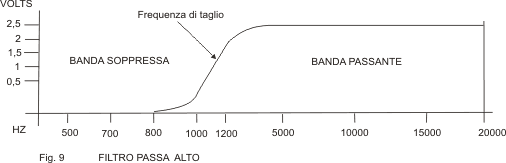
\includegraphics[width=0.6\textwidth]{./F_passa_alto.png}
  \caption{Esempio di un filtro passa alto \cite{SELET}}
 \end{figure}

\subsubsection{Filtro passa basso (low pass).}
Il filtro passa basso \`e esattamente l' opposto del filtro passa alto cio\`e permette il passaggio di una banda di frequenze al di sotto di una determinata frequenza limite. 

\begin{figure}[h]
 \centering
 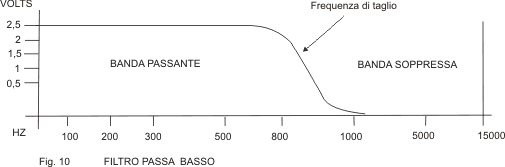
\includegraphics[width=0.6\textwidth]{./F_passa_basso.png}
 % F_passa_basso.png: 505x167 pixel, 72dpi, 17.81x5.89 cm, bb=0 0 505 167
  \caption{Esempio di un filtro passa basso \cite{SELET}}
\end{figure}



\subsubsection{Filtro passa banda (band pass).}
Il passa banda deriva dall'accoppiamento di un passa alto con un passa basso, quindi lascia passare solo una banda ristretta di frequenze che rientrano tra le frequenze di taglio dei due filtri accoppiati.
Comunque bisogna tener conto che al di sopra e al disotto di tali frequenze le altre componenti del segnale vengono eliminate, non in maniera netta, ma in modo graduale dipendente dalla "pendenza" della curva di selettivit\`a del filtro che varia a seconda del livello qualitativo del filtro stesso.

\begin{figure}[h]
 \centering
 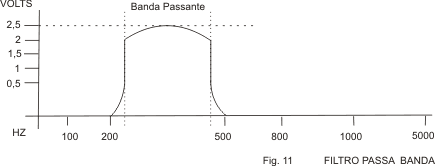
\includegraphics[width=0.6\textwidth]{./F_passa_banda.png}
 % F_passa_banda.png: 435x166 pixel, 72dpi, 15.34x5.86 cm, bb=0 0 435 166
 \caption{Esempio di un filtro passa banda \cite{SELET}}
 \end{figure}


\subsubsection{Filtro soppressore di banda (band reject).}
Il filtro a soppressione di banda \`e esattamente il contrario del filtro passa banda, in quanto pur essendo costituito dall'unione di un passa alto con un passa basso, respinge solo una ristretta banda di frequenze lasciando passare tutte le altre.

\begin{figure}[h]
 \centering
 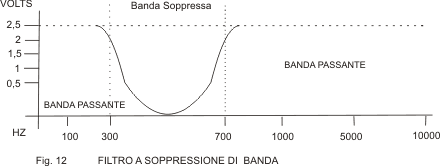
\includegraphics[width=0.6\textwidth]{./F_soppress_banda.png}
 % F_soppress_banda.png: 440x166 pixel, 72dpi, 15.52x5.86 cm, bb=0 0 440 166
 \caption{Esempio di un filtro soppressore di banda \cite{SELET}}
 \end{figure}

\section{Filtrare i suoni respiratori}
 
Entrando pi\`u nel dettaglio, durante l'analisi della letteratura attuale abbiamo riscontrato diversi tipi di filtri per l'eliminazione del rumore (denoising) e per eliminare il battito cardiaco.
L'eliminazione dei suoni emessi dal cuore \`e un problematica cruciale per il riconoscimento del respiro. 
Nello scenario previsto abbiamo un file audio del respiro preso grazie a uno stetoscopio elettronico; molti modelli di stetoscopi gi\`a concentono funzioni per filtrare il battito cardiaco, rilasciando quindi un suono a cui bisogna applicare solo un filtraggio per il denoising, per\`o nell'eventualit\`a in cui uno stetoscopio non sia fornito di queste funzioni bisogna trovare una tecnica di filtraggio ottimale che la maggior parte delle volte consiste nell'applicare piu di un filtro al suono che stiamo analizzando.
\newline
Si pu\`o subito notare attraverso l'analisi della letteratura approfondita nel capitolo 6, che il filtro usato maggiormente \`e quello passa banda, che permette di eliminare le frequenze che non rientrano nel range di frequenza dei suoni respiratori.
Per una migliore comprensione dell'analisi dei sistemi dei capitoli successi si andranno a illustrare alcune tecniche da loro usate.

\subsubsection{Downsampling }

Un filtro di downsampling o di sottocampionamento riduce la frequenza di campionamento di un segnale. Di solito lo scopo di questo filtro \`e di ridurre la complessit\`a computazionale dei successivi trattamenti del segnale. Il fattore di sottocampionamento \`e un numero intero o razionale maggiore di uno. Questo fattore moltiplica il tempo di campionamento o equivalentemente divide la frequenza di campionamento. Una implementazione di un filtro di sottocampionamento deve fare attenzione a non violare le condizioni del teorema sul campionamento di Shannon-Nyquist, altrimenti ci sar\`a la presenza di aliasing nel segnale di output. Questa tecnica viene usata sia da \cite{ASPODUOCSS} che da \cite{ASTFARA}.

\subsubsection{filtro mediano}

Il filtro mediano \`e un filtro non lineare ed \`e usato per la rimozione dei picchi di rumore dal segnale ed influenzano di solito solo una piccola percentuale dei campioni ma in modo notevole. L'idea principale di questo filtro \`e quella di rimpiazzare i campioni del segnale con la mediana dei campioni in una certo intervallo di campioni. Di solito questo intervallo si chiama finestra, la quale si muove su tutto il segnale campione per campione.

% \subsubsection{pacchetti wavelet}


\subsubsection{funzione finestra}
Nell'elaborazione numerica dei segnali una funzione finestra \`e una funzione che vale zero al di fuori di un certo intervallo. Quando un'altra funzione \`e moltiplicata per una funzione finestra, anche il prodotto assume valori nulli al di fuori dell'intervallo. Una definizione pi\`u generale di funzione finestra non richiede l'annullarsi al di fuori di un intervallo, ma che il prodotto per la funzione di finestra sia una funzione a quadrato sommabile, ovvero che la funzione finestra si annulli in maniera sufficientemente rapida. Le funzioni finestra sono importanti nel progetto dei filtri nell'analisi spettrale. 

% \paragraph{analisi spettrale}
% La trasformata di Fourier della fuzione $cos(\omega t)$ \`e zero tranne che alle frequenze $\pm \omega$. Quindi molte funzioni e forme d'onda non hanno una forma chiusa conveniente dalla trasformata. Alternativamente si potrebbe essere interessati nel contenuto spettrale durante un certo intervallo di tempo. In entrambi i casi, la trasformata di Fourier pu\`o essere applicata su uno o pi\`u intervalli finiti nella forma d'onda. In generale la trasformata \`e applicata al prodotto della forma d'onda e alla finestra. Ogni finestra influisce sulla stima spettrale calcolata con questo metodo. 
% 
% \paragraph{windowing}
% L'applicazione di una finestra ad una forma d'onda semplice come ad esempio $cos(\omega t)$ fa si che la sua trasformata di Fourier abbia valori diversi da zero in frequenze di verse da $\omega$. 
% If the waveform under analysis comprises two sinusoids of different frequencies, leakage can interfere with the ability to distinguish them spectrally. If their frequencies are dissimilar and one component is weaker, then leakage from the larger component can obscure the weaker one’s presence. But if the frequencies are similar, leakage can render them unresolvable even when the sinusoids are of equal strength.

% The rectangular window has excellent resolution characteristics for sinusoids of comparable strength, but it is a poor choice for sinusoids of disparate amplitudes. This characteristic is sometimes described as low-dynamic-range.
% 
% At the other extreme of dynamic range are the windows with the poorest resolution. These high-dynamic-range low-resolution windows are also poorest in terms of sensitivity; this is, if the input waveform contains random noise close to the frequency of a sinusoid, the response to noise, compared to the sinusoid, will be higher than with a higher-resolution window. In other words, the ability to find weak sinusoids amidst the noise is diminished by a high-dynamic-range window. High-dynamic-range windows are probably most often justified in wideband applications, where the spectrum being analyzed is expected to contain many different components of various amplitudes.
% 
% In between the extremes are moderate windows, such as Hamming and Hann. They are commonly used in narrowband applications, such as the spectrum of a telephone channel. In summary, spectral analysis involves a tradeoff between resolving comparable strength components with similar frequencies and resolving disparate strength components with dissimilar frequencies. That tradeoff occurs when the window function is chosen.Discrete-time signals
% 
% When the input waveform is time-sampled, instead of continuous, the analysis is usually done by applying a window function and then a discrete Fourier transform (DFT). But the DFT provides only a coarse sampling of the actual DTFT spectrum. Figure 1 shows a portion of the DTFT for a rectangularly windowed sinusoid. The actual frequency of the sinusoid is indicated as "0" on the horizontal axis. Everything else is leakage, exaggerated by the use of a logarithmic presentation. The unit of frequency is "DFT bins"; that is, the integer values on the frequency axis correspond to the frequencies sampled by the DFT. So the figure depicts a case where the actual frequency of the sinusoid happens to coincide with a DFT sample,[note 1] and the maximum value of the spectrum is accurately measured by that sample. When it misses the maximum value by some amount (up to 1/2 bin), the measurement error is referred to as scalloping loss (inspired by the shape of the peak). But the most interesting thing about this case is 
% that all the other samples coincide with nulls in the true spectrum. (The nulls are actually zero-crossings, which cannot be shown on a logarithmic scale such as this.) So in this case, the DFT creates the illusion of no leakage. Despite the unlikely conditions of this example, it is a common misconception that visible leakage is some sort of artifact of the DFT. But since any window function causes leakage, its apparent absence (in this contrived example) is actually the DFT artifact.
% 
% [edit]Noise bandwidth
% The concepts of resolution and dynamic range tend to be somewhat subjective, depending on what the user is actually trying to do. But they also tend to be highly correlated with the total leakage, which is quantifiable. It is usually expressed as an equivalent bandwidth, B. Think of it as redistributing the DTFT into a rectangular shape with height equal to the spectral maximum and width B.[note 2][4] The more leakage, the greater the bandwidth. It is sometimes called noise equivalent bandwidth or equivalent noise bandwidth, because it is proportional to the average power that will be registered by each DFT bin when the input signal contains a random noise component (or is just random noise). A graph of the power spectrum, averaged over time, typically reveals a flat noise floor, caused by this effect. The height of the noise floor is proportional to B. So two different window functions can produce different noise floors.
% 
% [edit]Processing gain
% In signal processing, operations are chosen to improve some aspect of quality of a signal by exploiting the differences between the signal and the corrupting influences. When the signal is a sinusoid corrupted by additive random noise, spectral analysis distributes the signal and noise components differently, often making it easier to detect the signal's presence or measure certain characteristics, such as amplitude and frequency. Effectively, the signal to noise ratio (SNR) is improved by distributing the noise uniformly, while concentrating most of the sinusoid's energy around one frequency. Processing gain is a term often used to describe an SNR improvement. The processing gain of spectral analysis depends on the window function, both its noise bandwidth (B) and its potential scalloping loss. These effects partially offset, because windows with the least scalloping naturally have the most leakage.



% Le finestre vengono usate spesso nel progetto dei filtri digitali, in particolare per convertire 
% Windows are sometimes used in the design of digital filters, in particular to convert an "ideal" impulse response of infinite duration, such as a sinc function, to a finite impulse response (FIR) filter design. That is called the window method.[5][6]


% \subsection{Esempi di finestre}

% \paragraph{terminologia}
% Usiamo $N$ per rappresentare l'ampiezza in numero di campioni di una finestra simmetrica $w(n)$. Se $N$ \`e un numero dispari, la finestra non-flat ha un unico punto singolare massimo. Se $N$ \`e pari, ha un doppio massimo. 
% La finestra cosidetta DFT-pari \`e asimmetrica e ha un solo massimo ma un numero pari di campioni(richiesti dall'algoritmo FFT). 
% Each figure label includes the corresponding noise equivalent bandwidth metric (B)[note 2], in units of DFT bins. As a guideline, windows are divided into two groups on the basis of B. One group comprises 1 ≤ B ≤ 1.8, and the other group comprises B ≥ 1.98. The Gauss, Kaiser, and Poisson windows are parametric families that span both groups, though only one or two examples of each are shown.
% Ci sono varie finestre ad esempio: finestra rettangolare \`e la pi\`u semplice, lascia invariati i campioni al suo interno e mette a zero gli altri. 
Siano $N$ l'ampiezza in numero di campioni di una finestra (tipicamente una potenza di 2) ed $n$ un numero intero, che assume valori da $0$ ad $N-1$. Ci sono varie funzioni finestre, ad esempio: 
  \begin{itemize}
    \item 
      la finestra rettangolare descritta dall'equazione 
      \[
	w(n)=1  
      \]
    \item
      la finestra di Hamming descritta dall'equazione
      \[
	w(n)=0.54-0.46 cos \left(\frac{2 \pi n}{N-1}\right)
      \]
      \`e stata progettata per minimizzare il livello del lobo laterale, mentre mantiene approssimativamente la stessa larghezza del lobo principale.
    \item
      la finestra di Hann o Hanning descritta dall'equazione:
      \[
	w(n)=0.5 cos \left(1-\frac{2 \pi n}{N-1}\right)
      \]
    \item
      la finestra di Blackmann descritta dall'equazione:
      \[
	w(n)=\frac{1-0.16}{2} - \frac{1}{2} cos \left(1-\frac{2 \pi n}{N-1}\right) + \frac{0.16}{2} cos \left(\frac{4 \pi n}{N-1}\right)
      \]
  \end{itemize}

% Other windows are designed to moderate these sudden changes because discontinuities have undesirable effects on the discrete-time Fourier transform (DTFT) and/or the algorithms that produce samples of the DTFT.[9][10]

% \paragraph{finestra di Hamming}

\if false

Un filtro digitale \`e una funzione su segnali digitali che ha vari scopi: rimuovere parti di un segnale(ad esempio estrae rumore casuale), modificare un segnale, estrarre parti utili del segnale(ad esempio quella parte del segnale che si trova all'interno di una specifica banda di frequenza). 
% I filtri sono quelle apparecchiature in grado di modificare il contenuto armonico di un segnale elettrico complesso.Queste modifiche si esprimono in termini di fasci di frequenze che vengono evidenziate o soppresse a secondo delle caratteristiche del tipo di filtro usato. A ad esempio con un filtro passa banda si pu\`o far passare da un rumore soltanto una determinata banda di frequenze sopprimendo tutte le altre. la fascia di frequenze passanti o banda passante, per alcuni filtri viene delimitata da una sola frequenza, mentre in altri da due, dette frequenze di taglio. Al di sopra e al disotto di tali frequenze le altre componenti del segnale vengono eliminate, non in maniera netta, ma in modo graduale dipendente dalla "pendenza" della curva di s


Se un filtro calcola l'output corrente solo dall'input precedente allora si chiama filtro non ricorsivo oppure filtro FIR(finite impluse response o risposta finita all'impulso). Invece se un filtro calcola l'output corrente solo dall'input precedente allora si chiama filtro ricorsivo o filtro IIR(infinite impulse response o risposta infinita all'impulso). 
La risposta all'impulso di un filtro digitale \`e la sequenza di output del filtro quanto la sequenza di input \`e impulso unitario. Un impulso unitario \`e un segnale di input che vale uno al tempo zero e poi vale sempre zero. 
Un filtro FIR ha un output di durata finita mentre un IIR ha un output di durata infinita. In pratica il termine IIR non \`e assolutamente accurato perch\'e la risposta di un filtro IIR tende spesso a zero. 
L'ordine di un filtro digitale non ricorsivo \`e il numero di input precedenti memorizzati per calcolare l'output corrente. L'ordine di un filtro ricorsivo \`e il pi\`u grande numero di input o output precedenti che il filtro usa per calcolare l'output corrente. 
Se abbiamo un filtro digitale non ricorsivo definito nel modo seguente: 
\[
  \sum_{i=0}^{n} a_{i} x_{i}
\] 
allora diciamo che $a_{i}$ \`e il coefficiente di indice $i$ del filtro. Definiamo il tempo di latenza di un filtro come la differenza di tempo tra l'input e la risposta.


Diciamo che un filtro $F$ \`e lineare se \`e un operatore lineare su un certo spazio di segnali, cio\`e se $r,s$ sono segnali e $a,b$ sono scalari allora 
\[
  F(ar + bs) = aF(r) + bF(s)
\]
Se questa propriet\`a non vale, diciamo che il filtro \`e non lineare. I filtri non lineari hanno importanti applicazioni ad esempio nella rimozione di rumore non additivo. 



I segnali spesso si degradano durante la trasmissione o il trattamento per questo motivo sono stati progettati dei filtri di rimozione del rumore. Il rumore pu\`o essere additivo, cio\`e al segnale S si aggiunge un segnale N non voluto che non ha nessuna relazione con S. Se il rumore N ha una descrizione statistica semplice come il rumore Gaussiano allora si pu\`o ridurre usando un filtro di Kalman. In particolare, se S e N non si sovrappongono nel dominio delle frequenze, possono essere separati completamente da un filtro lineare passa banda. 
Se il rumore \`e non additivo, invece, c'\`e bisogno di un filtro non lineare per ricostruire il segnale. Ad esempio nel caso del rumore moltiplicativo(rumore che viene moltiplicato dal segnale), pu\`o bastare una conversione dell'input in scala logaritmica, applicare un filtro lineare e convertire il risultato in scala lineare. 
Molti filtri non lineari per la rimozione del rumore operano nel dominio del tempo. Tipicamente esaminano il segnale di input in una finestra finita 
e usano un modello statistico di inferenza per stimare i valori pi\`u probabili per il segnale originale.



Supponiamo che il segnale di input sia una funzione nel tempo discreto $V=x(t)$. Il segnale \`e campionato respetto ad un intervallo di tempo $h$. Possiamo rappresentare il segnale anche come una sequenza di valori $x_{i}=x(ih)$.  Possiamo descrivere un filtro digitale attraverso una formula che descrive $y_{i}$ cio\`e l'output all'istante $i$ in funzione degli input e degli output precedenti $x_{0}, \cdots, x_{i}, y_{0}, \cdots, y_{i-1}$. Nei paragrafi successivi descriviamo alcuni tipi di filtri. Per maggiori dettagli si consulti ad esempio \cite{filtri}.
\subsection{Filtro simple gain}
    Questo filtro semplicemente moltiplica l'input per una costante: $y_{n} = K x_{n}$ dove $K$ \`e una costante. Se la costante \`e maggiore di $1$ allora parliamo di amplificatore, se la costante \`e compresa tra $0$ e $1$ allora parliamo di attenuatore, altrimenti se la costante \`e minore di $0$ parliamo di amplificatore inverso.
\subsection{Filtro ritardante}
    Questo filtro ritarda il segnale di un certo numero fisso di campioni: $y_{n} = x_{n-k}$ dove $k$ \`e un numero naturale. Nota che sebbene il primo campione del segnale sia $x_{0}$, il filtro produce un output significativo solo dopo $k$ campioni.
% \subsection{Filtro two-term difference filter}
%     Questo filtro restituisce la differenza tra un input e l'input precedente: $y_{n} = x+{n} - x_{n-1}$

\subsection{Filtro passa basso}% pi\`u semplice

Un filtro passa basso \`e un filtro che non cambia le frequenze basse e rifiuta le frequenze alte o meglio lascia passare il segnale nelle frequenze che vanno da $0Hz$ fino ad una certa frequenza di soglia mentre non lascia passare il segnale nelle frequenze maggiori della frequenza di soglia.

\subsection{Filtro passa alto}
Un filtro passa alto \`e un filtro che elimina o attenua la parte del segnale che ha una frequenza minore di una certa soglia mentre lascia invariata la parte del segnale con frequenze al di sopra di una certa soglia.





\subsection{Filtro mediano}

Il filtro mediano \`e usato per la rimozione dal segnale dei picchi di rumore, ed influenzano di solito solo una piccola percentuale dei campioni ma in modo notevole. Il filtro mediano \`e non lineare. L'idea principale del filtro mediano \`e di rimpiazzare i campioni del segnale con la mediana dei campioni in una certo intervallo di campioni. Di solito questo intervallo di chiama finestra, la quale si muove su tutto il segnale campione per campione. 


\subsection{Filtro di sottocampionamento}
Un filtro di downsampling o di sottocampionamento riduce la frequenza di campionamento di un segnale. Di solito lo scopo di questo filtro \`e di ridurre la complessit\`a computazionale di successivi eventuali trattamenti del segnale. Il fattore di sottocampionamento \`e un numero intero o razionale maggiore di uno. Questo fattore moltiplica il tempo di campionamento o equivalentemente divide la frequenza di campionamento. Una implementazione di un filtro di sottocampionamento deve fare attenzione a non violare le condizioni del teorema sul campionamento di Shannon-Nyquist, pena la presenza di aliasing nel segnale di output. 

% To ensure that the sampling theorem is satisfied, a low-pass filter is used as an anti-aliasing filter to reduce the bandwidth of the signal before the signal is downsampled; the overall process (low-pass filter, then downsample) is called decimation. Note that if the original signal had been bandwidth limited, and then first sampled at a rate higher than the Nyquist minimum, then the downsampled signal may already be Nyquist compliant, so the downsampling can be done directly without any additional filtering. Downsampling only changes the sample rate not the bandwidth of the signal. The only reason to filter the bandwidth is to avoid the case where the new sample rate would become lower than the Nyquist requirement and then cause the aliasing by being below the Nyquist minimum. Thus, in the current context of downsampling, the anti-aliasing filter must be a low-pass filter. However, in the case of sampling a continuous signal, the anti-aliasing filter can be either a low-pass filter or a band-pass filter. 
% A bandpass signal, i.e. a band-limited signal whose minimum frequency is different from zero, can be downsampled avoiding superposition of the spectra if certain conditions are satisfied, see e.g. [1].

\subsection{Filtro passa banda}
Un filtro passa banda ideale \`e un filtro che fa passare la parte del segnale che ha frequenze all'interno di un certo intervallo o banda e rifiuta la parte del segnale che ha frequenze che stanno al di fuori di questo intervallo. In pratica nessun filtro passa banda \`e ideale perch\'e esiste una regione al di fuori dell'intervallo di frequenza desiderato che non viene eliminata completamente ma solo attenuata. Indichiamo questa regione con il termine roll-off. L'intervallo di frequenze che il filtro fa passare viene chiamato banda passante.

\subsection{Filtro elimina banda}
Un filtro elimina banda o rifiuta banda \`e un filtro che attenua o elimina la parte del segnale che ha frequenza all'interno di un certo intervallo mentre lascia inalterato il segnale al di fuori di questo intervallo. Il filtro elimina banda e quello passa banda sono opposti.
% A notch filter is a band-stop filter with a narrow stopband (high Q factor).
% Narrow notch filters (optical) are used in Raman spectroscopy, live sound reproduction (public address systems, or PA systems) and in instrument amplifiers (especially amplifiers or preamplifiers for acoustic instruments such as acoustic guitar, mandolin, bass instrument amplifier, etc.) to reduce or prevent audio feedback, while having little noticeable effect on the rest of the frequency spectrum (electronic or software filters). Other names include 'band limit filter', 'T-notch filter', 'band-elimination filter', and 'band-reject filter'.
% Typically, the width of the stopband is 1 to 2 decades (that is, the highest frequency attenuated is 10 to 100 times the lowest frequency attenuated). However, in the audio band, a notch filter has high and low frequencies that may be only semitones apart.

\section{Envelope di un segnale}
\label{secSignalprocessingnvelope}

Dato un segnale nel dominio del tempo, diciamo che la sua envelope \`e una curva che varia molto meno rapidamente del segnale e che traccia il contorno di esso\cite{envelope}. La figura\ref{envelopeFig} illustra due envelope, una superiore e una inferiore, di un segnale sinusoidale.
\begin{figure}[h!]
 \centering
 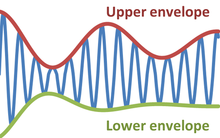
\includegraphics{./envelope.png}
 % envelope.png: 220x138 pixel, 96dpi, 5.82x3.65 cm, bb=0 0 165 104
  \label{envelopeFig}
\caption{Envelope superiore e inferiore di una onda sinusoidale\cite{envelopeImg}}
\end{figure}


\section{Funzione finestra}

Nell'elaborazione numerica dei segnali una funzione finestra \`e una funzione che vale zero al di fuori di un certo intervallo. Quando un'altra funzione \`e moltiplicata per una funzione finestra, anche il prodotto assume valori nulli al di fuori dell'intervallo. Una definizione pi\`u generale di funzione finestra non richiede l'annullarsi al di fuori di un intervallo, ma che il prodotto per la funzione di finestra sia una funzione a quadrato sommabile, ovvero che la funzione finestra si annulli in maniera sufficientemente rapida. Le funzioni finestra sono importanti nel progetto dei filtri FIR e nell'analisi spettrale. 

% \paragraph{analisi spettrale}
% La trasformata di Fourier della fuzione $cos(\omega t)$ \`e zero tranne che alle frequenze $\pm \omega$. Quindi molte funzioni e forme d'onda non hanno una forma chiusa conveniente dalla trasformata. Alternativamente si potrebbe essere interessati nel contenuto spettrale durante un certo intervallo di tempo. In entrambi i casi, la trasformata di Fourier pu\`o essere applicata su uno o pi\`u intervalli finiti nella forma d'onda. In generale la trasformata \`e applicata al prodotto della forma d'onda e alla finestra. Ogni finestra influisce sulla stima spettrale calcolata con questo metodo. 
% 
% \paragraph{windowing}
% L'applicazione di una finestra ad una forma d'onda semplice come ad esempio $cos(\omega t)$ fa si che la sua trasformata di Fourier abbia valori diversi da zero in frequenze di verse da $\omega$. 
% If the waveform under analysis comprises two sinusoids of different frequencies, leakage can interfere with the ability to distinguish them spectrally. If their frequencies are dissimilar and one component is weaker, then leakage from the larger component can obscure the weaker one’s presence. But if the frequencies are similar, leakage can render them unresolvable even when the sinusoids are of equal strength.

% The rectangular window has excellent resolution characteristics for sinusoids of comparable strength, but it is a poor choice for sinusoids of disparate amplitudes. This characteristic is sometimes described as low-dynamic-range.
% 
% At the other extreme of dynamic range are the windows with the poorest resolution. These high-dynamic-range low-resolution windows are also poorest in terms of sensitivity; this is, if the input waveform contains random noise close to the frequency of a sinusoid, the response to noise, compared to the sinusoid, will be higher than with a higher-resolution window. In other words, the ability to find weak sinusoids amidst the noise is diminished by a high-dynamic-range window. High-dynamic-range windows are probably most often justified in wideband applications, where the spectrum being analyzed is expected to contain many different components of various amplitudes.
% 
% In between the extremes are moderate windows, such as Hamming and Hann. They are commonly used in narrowband applications, such as the spectrum of a telephone channel. In summary, spectral analysis involves a tradeoff between resolving comparable strength components with similar frequencies and resolving disparate strength components with dissimilar frequencies. That tradeoff occurs when the window function is chosen.Discrete-time signals
% 
% When the input waveform is time-sampled, instead of continuous, the analysis is usually done by applying a window function and then a discrete Fourier transform (DFT). But the DFT provides only a coarse sampling of the actual DTFT spectrum. Figure 1 shows a portion of the DTFT for a rectangularly windowed sinusoid. The actual frequency of the sinusoid is indicated as "0" on the horizontal axis. Everything else is leakage, exaggerated by the use of a logarithmic presentation. The unit of frequency is "DFT bins"; that is, the integer values on the frequency axis correspond to the frequencies sampled by the DFT. So the figure depicts a case where the actual frequency of the sinusoid happens to coincide with a DFT sample,[note 1] and the maximum value of the spectrum is accurately measured by that sample. When it misses the maximum value by some amount (up to 1/2 bin), the measurement error is referred to as scalloping loss (inspired by the shape of the peak). But the most interesting thing about this case is 
% that all the other samples coincide with nulls in the true spectrum. (The nulls are actually zero-crossings, which cannot be shown on a logarithmic scale such as this.) So in this case, the DFT creates the illusion of no leakage. Despite the unlikely conditions of this example, it is a common misconception that visible leakage is some sort of artifact of the DFT. But since any window function causes leakage, its apparent absence (in this contrived example) is actually the DFT artifact.
% 
% [edit]Noise bandwidth
% The concepts of resolution and dynamic range tend to be somewhat subjective, depending on what the user is actually trying to do. But they also tend to be highly correlated with the total leakage, which is quantifiable. It is usually expressed as an equivalent bandwidth, B. Think of it as redistributing the DTFT into a rectangular shape with height equal to the spectral maximum and width B.[note 2][4] The more leakage, the greater the bandwidth. It is sometimes called noise equivalent bandwidth or equivalent noise bandwidth, because it is proportional to the average power that will be registered by each DFT bin when the input signal contains a random noise component (or is just random noise). A graph of the power spectrum, averaged over time, typically reveals a flat noise floor, caused by this effect. The height of the noise floor is proportional to B. So two different window functions can produce different noise floors.
% 
% [edit]Processing gain
% In signal processing, operations are chosen to improve some aspect of quality of a signal by exploiting the differences between the signal and the corrupting influences. When the signal is a sinusoid corrupted by additive random noise, spectral analysis distributes the signal and noise components differently, often making it easier to detect the signal's presence or measure certain characteristics, such as amplitude and frequency. Effectively, the signal to noise ratio (SNR) is improved by distributing the noise uniformly, while concentrating most of the sinusoid's energy around one frequency. Processing gain is a term often used to describe an SNR improvement. The processing gain of spectral analysis depends on the window function, both its noise bandwidth (B) and its potential scalloping loss. These effects partially offset, because windows with the least scalloping naturally have the most leakage.



% Le finestre vengono usate spesso nel progetto dei filtri digitali, in particolare per convertire 
% Windows are sometimes used in the design of digital filters, in particular to convert an "ideal" impulse response of infinite duration, such as a sinc function, to a finite impulse response (FIR) filter design. That is called the window method.[5][6]


% \subsection{Esempi di finestre}

% \paragraph{terminologia}
% Usiamo $N$ per rappresentare l'ampiezza in numero di campioni di una finestra simmetrica $w(n)$. Se $N$ \`e un numero dispari, la finestra non-flat ha un unico punto singolare massimo. Se $N$ \`e pari, ha un doppio massimo. 
% La finestra cosidetta DFT-pari \`e asimmetrica e ha un solo massimo ma un numero pari di campioni(richiesti dall'algoritmo FFT). 
% Each figure label includes the corresponding noise equivalent bandwidth metric (B)[note 2], in units of DFT bins. As a guideline, windows are divided into two groups on the basis of B. One group comprises 1 ≤ B ≤ 1.8, and the other group comprises B ≥ 1.98. The Gauss, Kaiser, and Poisson windows are parametric families that span both groups, though only one or two examples of each are shown.
% Ci sono varie finestre ad esempio: finestra rettangolare \`e la pi\`u semplice, lascia invariati i campioni al suo interno e mette a zero gli altri. 
$N$ rappresenta l'ampiezza, in numero di campioni, di una finestra a tempo discreto. Tipicamente \`e una potenza di 2. $n$ \`e un numero intero, che assume valori da $0$ ad $N-1$. Ci sono varie finestre ad esempio: 
\begin{itemize}
  \item 
    la finestra rettangolare descritta dall'equazione 
    \[
      w(n)=1  
    \]
  \item
    la finestra di Hamming descritta dall'equazione
    \[
    w(n)=0.54-0.46 cos \left(\frac{2 \pi n}{N-1}\right)
    \]
  \item
    la finestra di Hann o Hanning descritta dall'equazione:
    \[
      w(n)=0.5 cos \left(1-\frac{2 \pi n}{N-1}\right)
    \]
  \item
    la finestra di Blackmann descritta dall'equazione:
    \[
      w(n)=\frac{1-0.16}{2} - \frac{1}{2} cos \left(1-\frac{2 \pi n}{N-1}\right) + \frac{0.16}{2} cos \left(\frac{4 \pi n}{N-1}\right)
    \]
\end{itemize}

% Other windows are designed to moderate these sudden changes because discontinuities have undesirable effects on the discrete-time Fourier transform (DTFT) and/or the algorithms that produce samples of the DTFT.[9][10]

% \paragraph{finestra di Hamming}
\fi
\chapter{Tecniche risolutive}
\label{capitolo:preliminari:ulteriori}


% In questo capitolo si introducono le premesse teoriche necessarie per la comprensione dei capitoli successivi.
% Oltre alle tecniche riscontrate durante l'analisi della letteratura si \`e scelto di introdurre altri concetti utili per ulteriori metodi risolutivi.

Questo capitolo introduce le premesse teoriche necessarie per la comprensione di: 
\begin{itemize}
  \item 
    Algoritmi usati nello stato dell'arte.
  \item
    Algoritmi usati nel sistema implementato.
  \item
    Algoritmi dei quali \`e stata valutata l'adeguatezza alla soluzione del problema.
\end{itemize}

L'organizzazione dei contenuti in sezioni \`e illustrata nella figura \ref{prerequSect}
% Oltre alla presentazione degli algoritmi descritti nell'analisi della letteratura si \`e dato uno spazio alla descrizione di algoritmi utili per la soluzione del problema.
% Dopo un analisi delle possibili tecniche risolutive si \`e scelto di suggerire un sistema che utilizza un algoritmo di onset detection insieme a un algoritmo di clustering. 




\begin{center}
\begin{figure}
 

\begin{tikzpicture}
%   [scale=.8,auto=left,every node/.style={fill=blue!20}]
[->,>=stealth',shorten >=1pt,auto,node distance=3cm,
  thick,main node/.style={circle,fill=blue!20,draw,font=\sffamily\Large\bfseries}]
  \node (n1) at (0,3) {tecniche};

  \node (n1n1) at (4,1) {stato dell'arte};
  \node (n1n2) at (4,3) {sistema implementato};
  \node (n1n3) at (4,5) {altre valutate};

%   \node (N1) at (8,2) {filtri};
  \node (N2) at (8,3) {onset detection};
  \node (n1n1n2) at (8,2) {modelli markoviani};
  \node (n1n1n3) at (8,1) {dimensione frattale};
  \node (n1n3n1) at (8,4) {clustering};
  \node (n1n3n2) at (8,5) {reti neurali};

  \node (N1n1) at (12,3) {\ref{beatdetectionDescrizione}};
%   \node (N1n2) at (12,3) {\ref{filtri}};
  \node (n1n1n2n1) at (12,2) {\ref{markov}};
  \node (n1n1n3n1) at (12,1) {\ref{frattale}};
  \node (n1n3n1n1) at (12,4) {\ref{clustering}};
  \node (n1n3n2n1) at (12,5) {\ref{retineurali}};

   \foreach \from/\to in {n1/n1n1,n1/n1n2,n1/n1n3,n1n1/N2,n1n2/N2,n1n2/n1n3n1,n1n1/n1n1n2,n1n1/n1n1n3,n1n3/n1n3n1,n1n3/n1n3n2, N2/N1n1,n1n1n2/n1n1n2n1,n1n1n3/n1n1n3n1,n1n3n1/n1n3n1n1,n1n3n2/n1n3n2n1}
     \draw (\from) -- (\to);

\end{tikzpicture}
\caption{Organizzazione dei contenuti nelle sezioni del capitolo}
\label{prerequSect}
\end{figure}
\end{center}




\section{Beat detection}
\label{beatdetectionDescrizione}
% Con il termine beat detection intendiamo il riconoscimento del ritmo o del tempo di una musica a partire da una sua codifica digitale. 
Ad un livello intuitivo siamo tutti in grado di capire cos'\`e il ritmo e siamo anche in grado di capire qual'\`e il ritmo di una canzone quando l'ascoltiamo. 
% Esistono vari algoritmi di beat detection, alcuni dei quali cercano di mimare quei meccanismi naturali che ci permettono di seguire il tempo di una canzone.

% Il ritmo \`e il susseguirsi di una serie di accenti con una periodica regolarit\`a. Esso \`e basato sulla suddivisione del tempo in forme e misure variabili, talvolta regolari e simmetriche altre volte irregolari e asimmetriche. Il ritmo \`e quindi un movimento che si ripete regolarmente. 
Il ritmo \`e definito da una successione di accenti, intendendo con accento il maggior rilievo(variazione di intensit\`a, altezza o timbro) che alcuni suoni hanno rispetto ad altri nell'ambito di un brano o una frase musicale. La sequenza degli accenti di un brano musicale tende normalmente a ripetersi a intervalli regolari ed \`e questa ripetizione che viene chiamata ritmo del brano: la piu' breve sequenza non periodica(quella che viene ripetuta) viene anche chiamata cellula ritmica. Possiamo definire un onset come un accento importante alla caratterizzazione del ritmo. Per trovare il ritmo dobbiamo prima passare dagli onset.

% \cite{Bello} da le seguenti definizioni:
% \begin{description}
%   \item[attacco]
%     l'attacco di una nota \`e l'intervallo di tempo durante il quale aumenta l' amplitude envelope
%   \item[transient]
%     il transient \`e definito in modo informale come un breve intervallo di tempo durante il quale il segnale evolve rapidamente in modo non banale o in modo relativamente inprevedibile. Ad esempio quando si suona una nota in una chitarra classica il transient \`e il periodo che va da quando la corda viene pizzicata a quando la cassa risonanza smette di vibrare.
%   \item[onset]
%     l'onset di una nota un istante scelto per segnare un transient. Nella maggior parte dei casi coincide con l'inizio del transient cio\`e il momento nel quale il transient pu\`o essere rilevato in modo affidabile
% \end{description}
% Secondo \cite{Pekonen}, con il termine \emph{onset} nel contesto dell'audio digitale ci riferiamo all'inizio un evento temporale discreto in un segnale durante il quale avviene un cambiamento marcato di almeno una delle seguenti propriet\`a psicoacustiche: intensit\`a, altezza o timbro. Invece l'\emph{attacco} \`e l'intervallo di tempo nel quale l'ampiezza di un segnale aumenta. 
% 
% Come coinciliamo queste definizioni?






\if false

Fundamentally, music consists of sounds generated concurrently by a number of different sources
(usually musical instruments of varying kinds). These sources generally fall into two categories:
harmonic and percussive. The former produce sounds which would be regarded as notes, in that
they have an identifiable pitch and are made up of a series of harmonically related tones. Tones
are ideally periodic sine waves but in real instruments, non-linearities in the source (and deliberate
variations introduced by the performer) usually mean that they are only quasi-periodic [116]. The
pitch, which is a perceptual quality, is determined by the frequency of the fundamental tone and
the harmonic tones whose frequencies are approximately integer multiples of this fundamental2 .
The whole harmonic sound will have the same experiential pitch as a single sine wave at the
fundamental frequency [70]. The word partial is also used to describe the tones in a series. The
first partial is the fundamental, the second partial the first harmonic, and so on.
There are then two perceptual qualities associated with pitch: chroma and height [70]. In
Western music, the quality of chroma has been classified into twelve semitones labelled A to G
with five accidentals (sharps or flats). The twelfth semitone above any given note then has the
same chroma, but is greater in the percept of height. This is termed ‘octave equivalence’ and the
interval an octave (the eight comes from the concept of scales which are discussed below). Other
cultures have evolved other pitch classes, such as equally tempered seven note scales (South-East
Asia) and twenty two note scales (India) [41] but these will not be considered further here.
Next is the concept of the interval. This is a musical construction which relates notes of
different chroma to each other: for instance, a difference of four semitones is given the interval
label of ‘major third’ and ten semitones are a ‘minor seventh’. This is then one step away from
the concept of the scale, a series of notes arranged in ascending order and forming a perceptually
natural set, which when played together in patterns make chords as discussed below. Common
scales are the major and minor (though the latter has various accepted forms) which contain
seven separate chroma (hence the eighth or octave is the same as the first) and less common ones
include the pentatonic and jazz scales. The key or tonal context of a section of music is then the
scale which best fits the notes present [309].
The frequency relationships between the various chroma (i.e. intervals) were first investigated
by Pythagoras who compared the lengths of strings that formed consonant sounds when plucked
together [263]. Octaves were found to have a frequency ratio of 2:1; fifths, the ratio 3:2; fourths,
4:3; major third 5:4 etc. As an alternative to the Pythagorean scale, the ‘equal temperament’
scale is used predominantly today which divides the octave into twelve logarithmically spaced
semitones. This means that fourths and fifths especially are no longer rational ratios [88, 159]
but allows different keys to be played without discrepancies in tuning.
More recently with the advent of computer representations of music, numbers have also been
assigned to note pitches for ease of representation. The MIDI [289] note number (e.g. A3 = 69)
can be found from by the following equations which relate fundamental frequency f in Hertz3 to
a number, n:
Chords
In Western music, the concept of harmony has developed, where notes which sound concordant
together are formed into chords. The most simple combination of notes is the ‘major triad’ chord
which (in Pythagorean tuning) has the frequency ratio, 4:5:6. This takes the first note in the
chord along with the major third and fifth above it. The consonance comes from the fact that
every third harmonic of the first note will coincide in freqency with every second harmonic of
the third note. This commonality of harmonic content leads to a fused percept which listeners
find pleasing. The sharing of harmonics can be extended to give the concept of the root of a
chord: the note two octaves below the first note in the major triad has all three notes in the triad
as harmonics. Thus, given the triad of C-E-G, it explains why C is taken to be the root rather
than E or G [252]. Figure 2.1 shows the note relations of the harmonics of a root note. In equal
temperament, minor chords have the approximate relationship, 10:12:15 (6:7:9 is out of tune
[252]). The other two basic chords are the diminished and the augmented triads.
Other degrees of the scale can be added to produce chords with different feels: the 7th (either
major or minor) is a commonly added degree. In jazz, many different notes are added, both from
within the scale (e.g. 6th s, 9th s) and out of it (e.g. flattened 10th s, sharpened 13th s), which gives
jazz its characteristic feel.
Pitch Perception and Models
Krumhansl [191] has conducted extensive studies into scales and tonal context. She produced
profiles for each type of scale defining the perceptual match of each semitone within the tonal
context or mode. Dowling [101] gave another account of pitch perception with four levels: at
the top was a psychophysical function which reduced the continuous frequency range to a set
of discrete pitches; the second level incorporated cultural influences and set up a tonal context;
the third stage gave a tuning system, which was a subset within the tonal context suggested by
the excerpt in question; and finally the modal scale gave some of these selected pitches greater
perceptual weight.
Longuet-Higgins [206] noted that if a 2-D map of pitch relations was organised with 5th s
in one direction and major 3rd s in the other (being the prime factors of all intervals) then keys
could be realised in a compact set within the map. Balzano [14] gives a similar representation to
Longuet-Higgins and Shepard [301] devised yet another representation4 .
2.2.2 Percussive Sounds
Percussive sounds, in comparison, often lack harmonic structure and are more analogous to
noise clouds. The sound can be modelled as a stochastic signal and is usually characterised by a
broadband energy envelope. Drums and cymbals are the obvious examples of this class. These
sounds can still be classed in a pseudo pitch hierarchy: one sound can be classed as ‘higher’ or
‘lower’ than another. This is a reflection on the centre frequency of the noise cloud, though drums
such as timpani or tom-toms can be tuned to have a kind of pitch. However, the structure is not
harmonic in the same sense as described in §2.2.1. Bells are an example of a hybrid between
harmonic and percussive sounds. They exhibit a mostly inharmonic structure with no resonance
at or near the perceived fundamental. Instead, the pitch is determined by the 4th to 6th harmonics
[116]. Figure 2.2 shows time and frequency spectra for a single note with a harmonic (periodic)
structure and a snare drum hit which has a much more noise-like spectrum.
It should be noted that many (indeed most) harmonic instruments have a transient onset
which has much in common with percussive sounds. This is usually due to the excitation mech-
anism often producing a sound before the harmonic resonances are set up. Examples would be
the picking action of a guitar string or the breath noise at the start of a flute note.
2.2.3 Rhythm
Looking ahead, a large part of this thesis is devoted to rhythmic analysis and so it deserves
a comprehensive description. At the top level, the rhythm describes the timing relationships
between musical events within a piece. Indeed, the Oxford English Dictionary [321] gives the
definition of rhythm as
• a. The aspect of musical composition concerned with periodical accent and the duration of
notes.
• b. A particular type of pattern formed by this.
However, some further analysis can be made; Bilmes [26] breaks down rhythm into four subdi-
visions. The first is the hierarchical metrical structure which relates the idealised timing relation-
ships as they would exist in a musical score, i.e. quantised to a grid. Next is tempo variation
which gives the possibly time-varying speed at which the events are sounded. Another level of
abstraction gives timing deviations which are individual timing discrepancies around the overall
metrical grid (e.g. ‘playing ahead of the beat’; swing5 can also be considered a timing devia-
tion). Finally there are arrhythmic sections, where there is no established metre. These will be
ignored from now on as fundamentally impossible to analyse rhythmically, except as a collection
of unrelated note start times.
The metrical structure can also be broken down into a set of three hierarchical levels. Klapuri
[185] describes the beat, pulse or tactus as the preferred (trained) human tapping tempo. This
usually corresponds to the 1/4 note or crotchet when written out in common notation, though this
is not always the case: in fast jazz music, the pulse is often felt at half this rate (1/2 note or minim)
while hymns are often notated with the beat given in minims. At a lower level than the beat is the
tatum which is defined to be the shortest commonly occurring interval. This is often defined by the
1/8th notes (quavers) or 1/16th notes (semiquavers). Conversely, the main metrical level above the
beat is that of the bar or measure. This is related to the rate of harmonic change within the piece,
usually to a pattern of emphasis and also notational convention. Figure 2.3 gives a diagrammatic
representation of the above discussion. From here on, metrical levels below the beat, including
the tatum level will be termed the sub-beat structure while the converse, bar levels, etc., will
be labelled the super-beat structure. In between the tatum and beat, there may be intermediary
levels, usually related by multiples of two or three. The same applies between the beat and bar
levels. Gouyon [135] gives a comprehensive discussion of the semantics behind the words used to
describe rhythm, pointing out many of the dualities and discrepancies of terminology. One point
he raises is that the terms beat or pulse are used to describe both an individual element in a series
and the series as a whole.
An interesting point is raised by Honing [158] who discusses the duality between tempo
variations and timing: the crux of the problem is that a series of expressively timed notes can
be represented either as timing deviations around a fixed tempo, as a rapidly varying tempo
or any intermediate pairing. This is a fundamental problem in rhythm perception. Yeston [362]
investigated rubato, which is another term for a highly expressively timed performance, analysing
whether the tempo stayed constant at some higher metrical level.
Previously mentioned was the concept of the preferred human tapping tempo as the definition
of the beat. In engineering terms, however, the beat would best be described as a time varying
signal with frequency and phase, tempo corresponding to the frequency and a beat lying where
the phase is zero. Beat tracking is then the process of estimating this from the data. In the course
of this, assuming that the input is not isochronous (equal duration), an algorithm must perform
quantisation. This is the task of assigning a mis-timed or mis-estimated event to a position on the
metrical grid, a non trivial task in itself [49].
The phase of the beat is often determined by a series of stresses or accents, termed phenome-
nal accents [199, 253] or salience [90, 271]. It is generally assumed that stresses fall on the beat
more often than not and that significant chordal changes also do so. While this is not always
the case, and indeed many musical styles exhibit syncopation, where there are off-beat stresses,
Steedman notes, “No event inconsistent with either key or metre will occur in a piece until suf-
ficient framework (of key or time signature) has been established for it to be obvious that it is
inconsistent.” [310]
Psychology of Rhythm Perception
The psychology of rhythm perception is still little understood, though there have been two com-
peting schools of thought. The first is that of beat based timing, epitomised by the work of Povel
& Essens [271]. Here, the brain synchronises an internal clock to the perceived input and com-
pares each new event to this internal beat. The second proposal is interval timing whereby the
brain stores a representation of all the intervals it receives and then performs a comparison when
new intervals are received [177]. Opinion is divided on the subject and no conclusive proof of one
or the other exists to date, though it seems likely that perception is a combination of both [140].
Section 2.5 gives some of the beat perception models which have been proposed while §2.2.5
discusses some of the general music cognition models, which also include rhythmic aspects.
Related to the discussion is research on tapping in time to rhythms. Drake et al [102] inves-
tigated tapping to musical audio and found that while non-musicians were able to tap along ‘in
time with the music’, musicians were able to do so more accurately. Also, musicians were able to
tap at a greater variety of metrical levels (both above and below the beat) than non-musicians.

\fi
































% \section{Algoritmi di onset detection}

La maggior parte degli algoritmi di onset detection seguono uno schema assimilabile a quello illustrato nella figura \ref{onsetActivityDiagram} e descritto nelle sezioni seguenti.
\subsection{Preprocessing}
    Il concetto di preprocessing implica la trasformazione del segnale originale con lo scopo di accentuare o attenuare alcuni aspetti del segnale in base alla rilevanza che hanno nel dominio del problema. Questa fase \`e opzionale e ci sono vari modi di affrontarla ad esempio la separazione nelle frequenze. In questo caso l'informazione viene appunto separata in bande di frequenza.
% ma i due piu' importanti sono:
%     \begin{description}
%       \item[separazione nelle frequenze]
	


% 	Goto [3] slices the spectrogram into spectrum strips and recognizes onsets by detecting sudden changes in energy. These are used in a multiple-agent architecture to detect rhythmic patterns.
% 
% 	Scheirer [4] implements a six-band filter bank, using sixth-order elliptic filters, and psychoacoustically inspired processing to produce onset trains. These are fed into comb-filter resonators in order to estimate the tempo of the signal.
% 
% 	The second case is illustrated by models such as the perceptual onset detector introduced by Klapuri [5]. In this implementation, a filter bank divides the signal into eight nonoverlapping bands. In each band, onset times and intensities are detected and finally combined. The filter-bank model is used as an approximation to the mechanics of the human cochlea.
% 
% 	Another example is the method proposed by Duxbury et al. [6], that uses a constant-Q conjugate quadrature filter bank to separate the signal into five subbands. It goes a step further by proposing a hybrid scheme that considers energy changes in high-frequency bands and spectral changes in lower bands. By implementing a multiple-band scheme, the approach effectively avoids the constraints imposed by the use of a single reduction method, while having different time resolutions for different frequency bands.
%       \item[separazione transient steady state]
% 	La separazione dei transent dagli stati steady di solito \`e associato ad un modello del segnale musicale. Ci sono alcuni metodi che producono segnali modificati che possono essere usati per l'onset detection. Ad esempio i modelli sinusoidali, come quelli detti di sintesi additiva [7], rappresentano un segnale audio come una somma di sinusoidi con parametri che variano lentamente. 
% 
% 	Tra questi metodi Amongst these methods, spectral modeling synthesis (SMS) [8] explicitly considers the residual1 of the synthesis method as a Gaussian white noise filtered with a slowly varying low-order filter. 
% 
% 	Levine [9] calculates the residual between the original signal and a multiresolution SMS model. Significant increases in the energy of the residual show a mismatch between the model and the original, thus effectively marking onsets. 
% 
% 	An extension of SMS, transient modeling synthesis, is presented in [10]. Transient signals are analyzed by a sinusoidal analysis/synthesis similar to SMS on the discrete cosine transform of the residual, hence in a pseudo-temporal domain. 
% 	
% 	In [11], the whole scheme, including tonal and transients extraction is generalized into a single matching pursuit formulation.
% 
% 	An alternative approach for the segregation of sinusoids from transient/noise components is proposed by Settel and Lippe [12] and later refined by Duxbury et al. [13]. It is based on the phasevocoder principle of instantaneous frequency (see Section III-A.3) that allows the classification of individual frequency bins of a spectrogram according to the predictability of their phase components.
% 
% 	Other schemes for the separation of tonal from nontonal components make use of lapped orthogonal transforms, such as the modified discrete cosine transform (MDCT), first introduced by Princen and Bradley [14]. These algorithms, originally designed for compression [15], [16], make use of the relative sparsity of MDCT representations of most musical signals: a few large coefficients account for most of the signals energy. Actually, since the MDCT atoms are very tone-like (they are cosine functions slowly modulated in time by a smooth window), the part of the signal represented by the large MDCT atoms, according to a given threshold, can be interpreted as the tonal part of the signal [10], [17]. Transients and noise can be obtained by removing those large MDCT atoms.
%     \end{description}

\subsection{Reduction}
 \begin{wrapfigure}{r}{0.4\textwidth}
   \begin{center}
 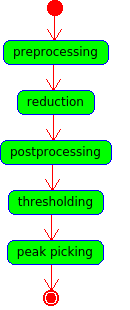
\includegraphics{./onsetActivityDiagram.png}
 % onsetActivityDiagram.png: 322x477 pixel, 96dpi, 8.52x12.62 cm, bb=0 0 241 358
   \end{center}
   \caption{Diagramma di attivit\`a di un generico algoritmo di beat detection}
   \label{onsetActivityDiagram}
 \end{wrapfigure}
    La riduzione \`e il processo di trasformare il segnale audio in un segnale con una frequenza di campionamento molto piu' ridotta e che manifesta in modo piu' evidente la posizione degli onset. Questo \`e il cuore degli algoritmi di onset detection. Chiamiamo l'output di questa fase anche detection function. Classifichiamo i metodi di riduzione in due categorie: metodi basati su caratteristiche esplicite del segnale e metodi basati su modelli probabilistici. 
    \paragraph{Metodi basati su caratterische esplicite del segnale.}
    Le caratteristiche esplicite di un segnale possono rientrare nelle categorie: temporali, spettrali, spettrali di fase e spettrotemporali. 
    \paragraph{Caratterische temporali.}
	Nel dominio del tempo del segnale si nota spesso che una occorrenza di un onset di solito \`e accompagnata da un aumento dell'ampiezza del segnale. Alcuni metodi di onset detection si avvantaggiano di questa propriet\`a e creano una detection function che segue l'envelope del segnale. Questi metodi danno risultati soddisfacenti nei casi in cui c'\`e un onset molto forte rispetto al sottofondo. 
%     \paragraph{caratterische spettrali} DA FARE
    \paragraph{Metodi basati su modelli probabilistici.}
      I metodi statici per l'onset detection sono basati sull'assunto che il segnale pu\`o essere descritto da qualche modello di probabilit\`a. Quindi si pu\`o costruire un sistema che fa inferenza probabilistica riguardo i tempi probabili di cambiamenti improvvisi nel segnale in base alle osservazioni disponibili. Il successo di questo approccio dipende dalla somiglianza tra la distribuzione di probabilit\`a descritta dal modello e la distribuzione reale dei dati e si pu\`o quantificare usando modelli di selezione Bayesiani. Ci sono vari metodi di questo tipo.

% background. A variation on this is to follow the local energy,
% rather than the amplitude, by squaring, instead of rectifying,
% each sample
% (2)
% Despite the smoothing, this reduced signal in its raw form is
% not usually suitable for reliable onset detection by peak picking.
% A further refinement, included in a number of standard onset
% detection algorithms, is to work with the time derivative of the
% energy (or rather the first difference for discrete-time signals) so
% that sudden rises in energy are transformed into narrow peaks in
% the derivative. The energy and its derivative are commonly used
% in combination with preprocessing, both with filter-banks [3]
% and transient/steady-state separation [9], [19].
% Another refinement takes its cue from psychoacoustics: em-
% pirical evidence [20] indicates that loudness is perceived loga-
% rithmically. This means that changes in loudness are judged rel-
% ative to the overall loudness, since, for a continuous time signal,
% . Hence, computing the first-dif-
% roughly simulates the ears perception of
% ference of
% loudness. An application of this technique to multiple bands [5]
% showed a significant reduction in the tendency for amplitude
% modulation to cause the detection of spurious onsets.
% 

%   \subsection{peak picking}
%     Se la detection function \`e stata progettata bene, allora gli onset danno luogo a caratterische ben localizzate e facilmente identificabili nella detection function. Di solito queste caratterische sono massimi locali o \emph{peak}, generalmente soggetti a qualche livello di variabilit\`a in forma e dimensione, e mascherati da rumore. Dunque un algoritmo robusto di scelta dei picchi ha bisogno di stimare il tempo di onset degli eventi nell'analisi del segnale. Dividiamo il processo di scelta dei picchi in tre fasi: 
  \subsection{Postprocessing}
	Questa fase \`e opzionale e serve per facilitare le fasi successive attraverso l'aumento dell'uniformit\`a e dela consistenza di alcuni aspetti della detection function che vengono trasformati in massimi locali isolati e facili da trovare. In questa fase possiamo trovare ad esempio: algoritmi di riduzione del rumore e algoritmi di selezione di parametri utili al calcolo del thresholding nelle fasi successive.

  \subsection{Thresholding}
	Ci possono essere dei picchi nella detection function che non sono correlati ad un onset di interesse. Quindi \`e necessario definire un threshold che separi in modo efficacie i picchi che corrispondono ad un evento di interesse e quelli che non vi corrispondono. In questa fase un onset che corrisponde ad un evento di interesse \`e definito come un picco nel quale la detection function supera una certa soglia. Ci sono due approcci principali alla scelta della soglia:
	\begin{description}
	  \item[Thresholding fisso.]
	    La soglia in questione non varia nel corso della vita dell'algoritmo.
	  \item[Thresholding adattativo.]
	    La soglia in questione varia ed \`e di solito una certa funzione della detection function. Ad esempio:
	    \begin{description}
	      \item[Linear smoothing.]
		La soglia \`e una combinazione lineare degli elementi all'interno della finestra corrente della detection function.
	      \item[Non linear smoothing.]
		La soglia \`e una combinazione non lineare degli elementi all'interno della finestra corrente della detection function. Ad esempio una combinazione dei quadrati.
	      \item[Percentiles smoothing.]
		I metodi precedenti hanno lo svantaggio che quando ci sono dei picchi relativamente grandi seguiti da picchi piccoli, questi ultimi vengono nascosti. Per evitare questo problema si posso usare metodi basati sui percentili ad esempio la mediana. 
	    \end{description}
	\end{description}
  \subsection{Peak picking}
    Nella fase di scelta dei picchi si devono solamente identificare i massimi locali al di sopra del threshold. 


% For a review of a number of peak-picking algorithms for audio signals, see \cite{TFTAAOMA}. 


% For our experiments the detection functions were first nor-
% malized by subtracting the mean and dividing by the maximum
% absolute deviation, and then low-pass filtered. An adaptive
% threshold, calculated using a moving-median filter [(21)], was
% then subtracted from the normalized detection function. Finally,
% every local maximum above zero was counted as an onset. Both
% the filter and the thresholding parameters (cutoff frequency,
% , and ) were hand-tuned based on experimenting, thus
% resulting in a separate parameter set for each detection function.
% Values for the cutoff frequency are selected according to the in-
% herent characteristics of each detection method, as discussed in section IIIC
% is set to the longest time interval on which the
% global dynamics are not expected to evolve (around 100 ms);
% while is set to 1, as it is not critical for the detection. However,
% experiments show sensitivity to variations of , such that error
% rates can be minimized by changing it between different types
% of music signals (e.g., pitched percussive, nonpercussive, etc).


 

% I metodi temporali nella fase di riduzione sono semplici e computazionalmente efficienti. Il loro funzionamento dipende dall'esistenza di aumenti chiaramente identificabili nell'ampiezza del segnale. La robustezza dei metodi basati sull'ampiezza diminuisce in presenza di modulazioni di ampiezza e di sovrapposizione di energie prodotte da suoni simultanei. Questo rimane vero anche se si divide il segnale in bande. 
% Per suoni non banali, gli schemi di onset detection beneficiano dell'uso di rappresentazioni piu' ricche del segnale(frequenza rispetto al tempo).  
% 
% The commonly used HFC [22, eq. (4)] is an example of a spectral weighting method. It is successful at emphasizing the percussiveness of the signal [cf. Figs. 5 and 6], but less robust at detecting the onsets of low-pitched and nonpercussive events [cf. Fig. 4], where energy changes are at low frequencies and hence de-emphasized by the weighting. 
% 
% In some signals, even broadband onsets are susceptible to masking by continuous high-frequency content such as that due to open cymbals in a pop recording. This problem can be overcome by using temporal difference methods such as the norm of the rectified spectral difference [[6, eq. (5)], as these can respond to changes in the distribution of spectral energy, as well as the total, in any part of the spectrum. However, the difference calculation relies solely on magnitude information, thus neglecting the detection of events without a strong energy increase: e.g., low notes, transitions between harmonically related notes or onsets played by
% bowed instruments (cf. Fig. 4). 
% 
% I metodi basati sulla fase, such as the spread of the distribution
% of phase deviations in (9) (see [25]), are designed to compensate for such shortcomings. They are successful at detecting low and high-frequency tonal changes regardless of their intensity. The approach suffers from variations introduced by the phases of noisy low-energy components, and from phase distortions common to complex commercial music recordings (e.g., audio effects, post-production treatments—cf. Fig. 6). The wavelet regularity modulus [29] in (12), is an example of an approach using an alternative time-scale representation that can be used to precisely localize events down to a theoretical resolution of as little as two samples of the original signal, which for typical audio sampling rates is considerably better than the ears resolution in time. The price of this is a much less smooth detec- tion function (cf. all figures), therefore emphasizing the need for post-processing to remove spurious peaks. The method provides an interesting alternative to other feature-based methods, but with an 
% increase in algorithmic complexity. Approaches based on probabilistic models provide a more general theoretical view of the analysis of onsets. As shown in Section III-B.2, previous reduction methods can be explained within the context of measuring surprise relative to a proba- bilistic model, while new methods can be proposed and evaluated by studying refinements or alternatives to existing models. An example is the surprise-based method using ICA to model the conditional probability of a short segment of the signal, calculated in (17) as the difference between two negative log-likelihoods [35]. If the model is adequate (i.e., the assumptions be- hind the model are accurate and the parameters well-fitted), then robust detection functions for a wide range of signals can be pro- duced. Examples are at the bottom of Figs. 4–6. However, for adaptive statistical models such as ICA, these advantages accrue only after a potentially expensive and time-consuming training process during which the parameters of the 
% model are fitted to a given training set.
% 






% \chapter{Online onset detection model}
% \cite{TFTAAOMA}:




\section{Clustering}
\label{clustering}
Il clustering \`e il processo di trovare informazioni strutturali all'interno di un insieme di dati. 
I meccanismi di clustering separano e organizzano dati non etichettati in vari gruppi o cluster, ognuno dei quali contiene dati che sono simili tra loro. 
Un buon algoritmo di clustering produce cluster nel quale la somiglianza intracluster, cio\`e tra gli elementi di un cluster, \`e alta mentre la somiglianza intercluster, cio\`e tra elementi di cluster diversi, \`e bassa. 
Per una discussione approfondita sul clustering si rimanda a \cite{PatternRecognition}.

Se vogliamo essere piu' formali possiamo dire che un $m-clustering$ di un insieme di dati $X$ rispetto ad una distanza o misura di dissimilarit\`a $d:P(X)\rightarrow \mathbb{R}$ e ad una soglia $t$ \`e $C_{1}, \cdots, C_{n}$ tale che:
\begin{description}
  \item[partizione]
    $C_{1}, \cdots, C_{n}$ \`e una partizione di $X$ cio\`e: ogni $C_{i}$ \`e un sottoinsieme di $X$; i $C_{i}$ sono a due a due disgiunti; l'unione dei $C_{i}$ d\`a $X$
  \item[intersimilarit\`a]
    per ogni $i$: $d(C_{i})<t$
\end{description}



  
Di seguito descriveremo alcuni tipi di algoritmi di clustering. 
Ci sono due tipi principali di algoritmi di clustering a seconda dei parametri di input. 
Una categoria di algoritmi prende in input il numero di cluster, oltre che gli elementi di input e la funzione di dissimilarit\`a, e restituisce un clustering dei dati. 
Una seconda categoria di algoritmi prende in input un valore di soglia e restituisce un clustering.
\paragraph{Clustering sequenziale.}
  Questi algoritmi leggono gli elementi di input uno per volta in sequenza. 
  In questo tipo di algoritmi non conosciamo a priori il numero di cluster presenti nell'input. 
  Invece prendono in input una soglia $\theta$ e il massimo numero di cluster permessi $q$. 
  L'idea alla base di questi algoritmi \`e che quando viene letto un elemento, questo viene o assegnato ad un cluster esistente o ad un nuovo cluster a seconda della distanza tra l'elemento e i cluster esistenti. 
  Uno schema generale per implementare un algoritmo di clustering sequenziale \`e dati in figura \ref{clusteringSequenzialeAlgoritmo}.

\incmargin{1em}
\restylealgo{boxed}\linesnumbered
\begin{algorithm}
  \dontprintsemicolon
  \SetVline
  % \SetNoline
%   \SetKwData{b}{b}
%   \SetKwData{This}{this}
%   \SetKwData{Up}{up}
  \SetKwFunction{getAverageLocalEnergy}{getAverageLocalEnergy}
  \SetKwFunction{getInstantSoundEnergy}{getInstantSoundEnergy}
  \SetKwFunction{Write}{write}
  \SetKwFunction{Init}{init}
  \SetKwFunction{Clear}{clear}
  \SetKwFunction{Add}{add}
  \SetKwFunction{DDDD}{distance}
  \SetKwInOut{Input}{input}
  \SetKwInOut{Output}{output}
  \caption{Sequential clustering algorithm}
    \Input{A sequence of data $x_{1}, \cdots, x_{n}$}
    \Output{A clustering of the data $C_{1}, \cdots, C_{m}$}
    \BlankLine
    $m\leftarrow 1$\;
    $C_{m}\leftarrow \{x_{1}\}$\;
    \For{$i\leftarrow 2$ \KwTo $n$}{
      find $k$ such that the distance between $x_{i}$ and $C_{k}$ is minimum\;
       \eIf{$\DDDD(x_{i}, C_{k}) > $ threshold}{
 	increments $m$\;
 	$C_{m}\leftarrow \{x_{i}\}$\;
       }{
 	$C_{m}\leftarrow C_{m}\cup \{x_{i}\}$\;
       }
  }
\label{clusteringSequenzialeAlgoritmo}
\end{algorithm}
\decmargin{1em}

Un algoritmo di clustering sequenziale si dice \emph{a cluster sequenziali} se produce cluster sequenziali e cio\`e \`e tale che ad ogni iterazione: o si aggiunge l'elemento corrente nello stesso cluster dell'iterazione precedente, o si aggiunge l'elemento in un nuovo cluster.

Se non si conosce in anticipo neanche il valore di soglia allora si pu\`o stimare il numero di cluster che ci sono nell'input usando l'algoritmo \ref{determinareClusterN}. 

\incmargin{1em}
\restylealgo{boxed}\linesnumbered
\begin{algorithm}
  \dontprintsemicolon
  \SetVline
  % \SetNoline
%   \SetKwData{b}{b}
%   \SetKwData{This}{this}
%   \SetKwData{Up}{up}
  \SetKwFunction{getAverageLocalEnergy}{getAverageLocalEnergy}
  \SetKwFunction{getInstantSoundEnergy}{getInstantSoundEnergy}
  \SetKwFunction{Write}{write}
  \SetKwFunction{Init}{init}
  \SetKwFunction{Clear}{clear}
  \SetKwFunction{Add}{add}
  \SetKwFunction{DDDD}{distance}
  \SetKwInOut{Input}{input}
  \SetKwInOut{Output}{output}
  \caption{Algoritmo di stima del numero dei cluster. Usato nella sezione \ref{clusteringMetodologia}}
    \Input{A sequence of data $x_{1}, \cdots, x_{n}$}
    \Output{An estimation of the number of clusters}
    \BlankLine
    \For{threshold $\leftarrow$ a \KwTo b step c}{
      run clustering algorithm with current threshold\;
      store the number of clusters obtained\;
    }
    \Return the most frequent number of clusters\;
\label{determinareClusterN}
\end{algorithm}
\decmargin{1em}



\paragraph{Clustering gerarchico.}
Il clustering gerarchico \`e un approccio di clustering che mira a costruire una gerarchia di cluster. 
Le strategie per il clustering gerarchico sono tipicamente di due tipi:
\begin{description}
  \item[Agglomerativo] 
    questo tipo di algoritmo produce una sequenza di clustering che hanno numero di cluster decrescente. 
  \item[Divisivo]
    questo tipo di algoritmo produce una sequenza di clustering che hanno numero di cluster crescente. 
    Ad ogni iterazione un algoritmo di questo tipo prende i cluster risultati dall'iterazione precedente e li divide.
\end{description}


\paragraph{Algoritmi di clustering basati su una funzione di ottimizzazione del costo.}
In questi algoritmi il numero di cluster \`e fisso. 
Si cerca di assegnare gli elementi di input ai cluster in modo da ottimizzare il valore di una funzione di costo. 



% Provare: 
%   mantenere il massimo e il minimo dell'energia di una finestra di 10ms
%   se l'energia di una finestra \`e maggiore dell'ottanta per cento del massimo allora \`e un beat, se \`e minore del 120 per cento  del minimo allora \`e silenzio
%   il respiro \`e beat seguito da non beat



% provare: 
% vari thread di esecuzione, ognuno un k clustering online sequenziale, k va da 1 a 10, quello che raggiunge una maggiore qualit\`a di clustering \`e l'algoritmo corretto
\section{Reti neurali}
\label{retineurali}
Le \emph{reti neurali artificiali} sono modelli matematici e computazionali della corteccia cerebrale. 
Gli elementi di base di una rete neurale artificiale sono:
\begin{description}
  \item[neuroni artificiali o unita']
%     neuroni artificiali o \emph{unita'} 
  \item[collegamenti]
    I neuroni artificiali sono connessi attraverso \emph{collegamenti}. 
    Ogni collegamento ha un \emph{peso} numerico, in particolare il collegamento tra l'unita' $i$ e l'unita' $j$ ha peso $w_{i,j}$. 
\end{description}
Una certa unita' $i$ pu\`o inviare un \emph{segnale} o \emph{attivazione} $a_{i}$ su tutti i suoi collegamenti. 
Il peso di un collegamento determina la forza e il segno del segnale. 
Assumiamo l'esistenza di una certa unita' di input che manda il segnale $a_{0}$. 
Ogni unita' si comporta nel modo seguente:
\begin{enumerate}
  \item 
    calcola la somma pesata dei suoi input
    \begin{center}
      $in_{j} = \sum\limits_{i=0}^n w_{i,j} a_{i}$
    \end{center}
  \item
    calcola il proprio output in base al valore calcolato al punto precedente e ad una \emph{funzione di attivazione} $g$: 
    \begin{center}    
      $a_{j}=g(in_{j})$
    \end{center}    
\end{enumerate}
La funzione di attivazione di solito \`e una funzione del tipo:
\begin{center}
  \begin{tabular}{lll}
      $g(x)= \left\{ 
	  \begin{array}{ll}
	      0
	    &
	      if\; x< 0
	    \\
	      1
	    &
	      if\; x> 0
	  \end{array}
      \right.$
    &
      o
    &
      $g(x)= \frac{1}{1+e^{-x}}$
  \end{tabular}
\end{center}

Ci sono due tipi di reti neurali:
\begin{description}
  \item[feed forward]
    I collegamenti tra unita' sono unidirezionali. 
    In questo caso la rete neurale \`e un grafo diretto aciclico. 
    Una rete neurale di tipo feed forward rappresenta una funzione dei suoi input nel senso che non ha uno stato interno o memoria. 
    Una rete feed forward \`e di solito divisa in \emph{layers} o livelli. 
    Ogni livello \`e un insieme di unita', ogni unita' riceve input solo da unita' del livello immediatamente precedente. 
    Una rete con un solo livello si dice anche \emph{single-layer} o \emph{monolivello}.
  \item[recurrent network]
    Ci possono essere dei cicli nei collegamenti. 
    Una rete di questo tipo rappresenta un sistema dinamico che pu\`o anche oscillare o avere un comportamento caotico. 
    Inoltre la riposta di una recurrent network dipende dallo stato iniziale della rete e dall'input quindi questo tipo di rete pu\`o supportare una memoria a breve termine.
\end{description}


\section{Dimensione frattale}
\label{frattale}
In geometria frattale la dimensione frattale \`e una quantit\`a statistica che da una indicazione di quanto completo appare un frattale per riempire lo spazio. 
La dimensione frattale inoltre \`e una misura della complessit\`a di un insieme di dati. 
Viene usata per analizzare segnali in un vasto numero di ricerche scientifiche. 
Una propriet\`a della dimensione frattale \`e che \`e indipendente dal contenuto di energia nel segnale ma \`e dipendente dalle frequenze. 
Ci sono molti modi di definire matematicamente la dimensione frattale ad esempio quello illustrato in \cite{RSDUVFD}:
\[
  D_{\sigma} = \displaystyle\lim_{\delta t \rightarrow 0} \frac{\log(Var(\delta S, \delta t))}{2 \cdot \log(\delta t)}
\]
In questa formula: $\delta t$ \`e il valore assoluto di una variazione temporale $|t_{2}-t_{1}|$ mentre $\delta S$ \`e la variazione del segnale nel tempo $S(t_{2})-S(t_{1})$.



 
\section{Catene di triple Markoviane}
\label{markov}
\subsection{Nozioni di base di probabilit\`a}

\paragraph{Evento. Spazio Campionario.}Dato un esperimento casuale, definiamo un evento elementare $\omega$ come uno dei possibili esiti dell'esperimento stesso. Definiamo un evento come un qualsiasi insieme di eventi elementari. Definiamo lo spazio campionario come l'insieme di tutti gli eventi elementari. Uno spazio campionario si indica di solito con il nome $\Omega$.

\paragraph{$\sigma-$algebra}
Dato un insieme $\Omega$, si definisce $\sigma-$algebra su $\Omega$ una famiglia $F$ di sottoinsiemi di $\Omega$ tale che:
\begin{itemize}
  \item 
    $\Omega$ appartiene ad $F$.
  \item
    L'insieme $F$ \`e chiuso rispetto a complementare.
  \item
    L'insieme $F$ \`e chiuso rispetto ad unione numerabile.
\end{itemize}.

\paragraph{Spazio misurabile. Insiemi misurabili.}
Uno spazio misurabile \`e una coppia $(\Omega, F)$ tale che $F$ \`e una $\sigma-$algebra su $\Omega$. Gli elementi di $F$ sono detti insiemi misurabili in $\Omega$.

\paragraph{Topologia. Spazio topologico.}
Dato un insieme $X$, una topologia su $X$ \`e un insieme $T$ di sottoinsiemi di $X$ tale che:
\begin{itemize}
  \item 
    L'insieme vuoto e $X$ appartengono a $T$.
  \item
    L'unione di una quantit\`a arbitraria di insiemi appartenenti a $T$ appartiene a $T$.
  \item
    L'intersezione di un numero finito di insiemi appartenenti a $T$ appartiene a $T$.
\end{itemize}
Uno spazio topologico \`e una coppia $(X, T)$, dove $X$ \`e un insieme e $T$ \`e una topologia su $X$. In uno spazio topologico gli insiemi che costituiscono $T$ si dicono aperti in $X$.

\paragraph{Funzione misurabile.}
Sia $(X,F)$ uno spazio misurabile e $(Y,T)$ uno spazio topologico. Una funzione $f:X\rightarrow Y$ viene detta misurabile se la controimmagine di ogni elemento di $T$ \`e in $F$.


\paragraph{Variabile casuale o aleatoria.}
Sia dato uno spazio campionario $\Omega$ su cui \`e definita una misura di probabilit\`a $\nu$, una variabile casuale \`e una funzione misurabile dallo spazio campionario a uno spazio misurabile. 


\paragraph{Processo stocastico.}
Si definisce processo stocastico una famiglia di variabili aleatorie  
\[
  \{X(T)|\; t\in T\subseteq \mathbf{R}^{+}\}
\]
dipendenti dal tempo, definite su un unico spazio campione $\Omega$ finito e che assumono valori in un insieme definito spazio degli stati del processo. Un processo stocastico \`e quindi un insieme di funzioni che evolvono nel tempo, ognuna delle quali \`e associata ad un determinato elemento dello spazio campione, cos\`i che il risultato di un esperimento casuale corrisponde di fatto all'estrazione di una di queste funzioni.
Un processo stocastico discreto \`e un processo stocastico nel quale $T$ \`e un sottoinsieme dei numeri naturali.


\subsection{Processo di Markov}
Un processo stocastico markoviano o processo di Markov \`e un processo stocastico nel quale la probabilit\`a di transizione che determina il passaggio ad uno stato di sistema dipende unicamente dallo stato di sistema immediatamente precedente (propriet\`a di Markov) e non dal come si \`e giunti a tale stato. Formalmente questo pu\`o essere scritto come
\[P(X_{n+1}\leq x_{n+1} |_{i=1}^{n} X_{i}\leq x_{i}) = P(X_{n+1}\leq x_{n+1} | X_{n}\leq x_{n})\]
Questa \`e detta propriet\`a di Markov, o condizione di assenza di memoria.

\subsection{Catena di Markov}
Una catena di Markov \`e un processo di Markov con spazio degli stati discreto, quindi si tratta di un processo stocastico che assume valori in uno spazio discreto e che gode della propriet\`a di Markov. L'insieme  di spazio degli stati pu\`o essere finito o infinito (numerabile). Nel primo caso si parla di catena di Markov a stati finiti. Una catena di Markov pu\`o essere tempo-continua o tempo-discreta, in base all'insieme di appartenenza della variabile tempo (continuo o discreto).
Formalmente, una catena di Markov \`e una sequenza di variabili aleatorie $X_{1}, X_{2}, \cdots, $ che soddisfa la condizione di Markov.


\subsection{Modelli nascosti di Markov}

In un modello nascosto di Markov abbiamo due processi stocastici: il processo di interesse inosservabile $X=(X_{s})_{s\in S}$ e il processo osservabile $Y=(Y_{s})_{s\in S}$. Un modello nascosto di Markov \`e $(X, Y, T, E, \pi)$ tale che:
\begin{description}
  \item
    $T:X\times X\rightarrow [0;1]$ \`e la probabilit\`a di transizione. In particolare 
    \[	
      p(X_{t+1}=x_{i}| X_{t}=x_{j})=T(x_{i},x_{j})
    \] 
    \`e la probabilit\`a che il processo nascosto passi dallo stato $x_{i}$ allo stato $x_{j}$.
  \item
    $E:X\times Y \rightarrow [0;1]$ \`e la probabilit\`a condizionata di $X$ rispetto ad $Y$. Cio\`e se osserviamo un certo valore $y$ per il processo osservabile $Y$ allora $E$ ci dice qual'\`e la probabilit\`a che il processo nascosto assuma certi valori.
  \item
    $\pi:X\rightarrow [0;1]$ \`e la probabilit\`a iniziale che il processo nascosto si trovi in un certo stato.
\end{description}






\subsection{Catena di coppie markoviane}


Supponiamo che $X = (X_{1}, \cdots, X_{n})$ e $Y = (Y_{1}, \cdots, Y_{1})$ siano due processi stocastici, nei quali ogni $X_{i}$ ha valori in un insieme finito $\Omega=\{\omega_{1}, \cdots, \omega_{n}\}$ e ogni $Y_{i}$ ha valori reali. Sia $Z = (Z_{1}, \cdots, Z_{n})$ il processo stocastico delle coppie di $X,Y$, cio\`e $Z_{i}=(X_{i}, Y_{i})$. 
I processi $X$ e $Y$ sono una catena di coppie markoviane se $Z$ \`e un processo di Markov cio\`e quando 
\[
  p(z)=p(z_{1}) p(z_{2}|z_{1}) \cdots p(z_{n}|z_{n-1})
\]



\subsection{Catena di triple markoviane}

Le catene di triple markoviane sono una estensione delle catene di coppie di Markov nelle quali la distribuzione di probabilit\`a di $(X,Y)$ \`e una distribuzione di probabilit\`a marginale di una catena di Markov $(X,U,Y)$.
Anche nelle catene di triple markoviane cerchiamo $X$ a partire da $Y$, il processo $S$ serve solo come aiuto al calcolo. 
Sia $S=N$ l'insieme dei numeri naturali senza lo zero e siano $X=(X_{n})_{n\in N}$, $Y=(Y_{n})_{n\in N}$, $U=(U_{n})_{n\in N}$ tre processi, nei quali le variabili $X_{i}$ assumono valori in uno spazio campionario $\Omega=\{\omega_{1}, \cdots, \omega_{k}\}$, le variabili $Y_{i}$ sono a valori reali e le variabili $U_{i}$ assumono  
valori nell'insieme $\Lambda = \{\lambda_{1}, \cdots, \lambda_{m}\}$.
Con lo scopo di semplificare la notazione, poniamo $T_{n}=(X_{n}, U_{n}, Y_{m})$, $Z_{n}=(X_{n}, Y_{n})$ e $V_{n}=(X_{n}, U_{n})$ e chiamiamo $T,Z$ e $V$ i processi corrispondenti.
Diremo che $Z$ \`e una catena di triple di Markov se esiste un processo $U$ nel quale $T$ \`e una catena di Markov.
In questo caso allora $(V,Y)$ \`e una catena di Coppie di Markov. Possiamo scrivere la distribuzione di probabilit\`a di $(V_{i}, Y)$ come 
\[
  p(v_{i}, y)=\alpha^{i}(v_{i}) \beta^{i}(v_{i})
\]
con $\alpha^{i}(v_{i})$ e $\beta^{i}(v_{i})$ definite rispettivamente come 
\[
  \begin{array}{ll}
      \alpha^{i}(v_{i})=p(y_{1}, \cdots, y_{i-1}, y_{i}, v_{i})
    &
      \beta^{i}(v_{i})=p(y_{i+1}, \cdots, y_{n}, v_{i}, y_{i})
  \end{array}
\]



% \chapter{Phoneme Recognition Using Time Delay Neural Networks}
Per essere utile per il riconoscimento vocale, una rete neurale feedforward deve avere un certo numero di proprieta'.
Primo, deve avere piu' livelli e un numero sufficiente di interconnessioni tra le unita' in ogni livello.
Questo per assicurasi che la rete neurale avra' l'abilita' di imparare superfici di decisione complesse non lineari.
Secondo, la rete deve avere l'abilita' di rappresentare relazioni tra gli eventi nel tempo.
Questi evento possono essere coefficienti spettrali ma possono essere anche il risultato di elaborazioni di aspetti piu' di alto livello.
Terzo, gli aspetti e le astrazioni imparate dalla rete neurale dovrebbero essere invarianti per traslazione nel tempo.
Quarto, la procedura di apprendimento non dovrebbe richiedere un allineamento temporale preciso delle etichette che si devono imparare.
Quinto, il numero di pesi nella rete dovrebbe essere sufficientemente piccolo in confronto alla quantita' di dati di allenamento cosi' che la rete deve codificare l'allenamento attraverso l'estrazione di regolarita'
Nel seguito descriviamo una architettura di una TDNN che soddisfa tutti questi criteri ed e' progettata esplicitamente per il riconoscimento dei fonemi, in particolare i voiced stops B D e G.
L'unita' di base usata in molte reti neurali calcola la somma pesata dei suoni input e dopo passa questa somma attraverso una funzione non lineare, di solito una soglia o una funzione sigmoide.
Nella nostra RDNN, questa unita' di base e' modificata introducendo ritardi da $D_{1}$ a $D_{n}$.
I $J$ input di questa unita' vengono poi moltiplicati da molti pesi, uno per ogni ritardo e uno per ogni inpit non ritardato.
Per $N=2$ e $J=16$, per esempio, c'e' bisogni di $48$ pesi per calcolare la somma pesata dei $16$ inputs, con ogni input misurato in tre punti diversi nel tempo.
In questo modo, una unita' di TDNN ha l'abilita' di relazionare e di confrontare l'input corrente con gli eventi passati.
La funzione sigmoide F e' stata scelta non lineare per via delle sue proprieta' matematiche.
Per il riconoscimento dei fonemi viene costruita una rete a tre livelli.
L'input della rete sono 16 coefficienti spettrari normalizzati ?melscale?.
Il segnale vocale, campionato a $12kHz$, passa attraverso una finestra di Hamming e una trasformata discreta di fourier di $256$ punti ogni $5ms$.
Ogni coefficiente melscale e' dato dal logaritmo dell'energia in una certa banda di energia melscale, nella quale coefficienti adiacenti nelle frequenze si sovrappongono di un campione spettrale e vengono smoothed attraverso la riduzione dei frequenzi cnodivisi del $50\%$.
Coefficienti adiacenti nel tempo vengono collassati per essere ridotti ulteriormente in una frame rate di $10ms$.
Tutti i coefficienti di un token di input(in questo caso $15$ frames vocail centrati attorno l'onset delle vocali etichettato a mano)
Questo si puo realizzare attraverso la sottrazione da ogni coefficiente della energia media dei coefficienti calcolata su tutte le $15$ frame di un token di input e poi normalizzare ogni coefficiente per stare tra $-1$ e $1$.
Tutti i token nel nostro database vengono trattati nello stesso modo.
% Fig. 2 shows the resulting coefficients for the speech token “BA” as input to the network, where positive values are shown as black squares and negative values as gray squares.

This input layer is then fully interconnected to a layer of 8 time-delay hidden units, where J = 16 and N = 2 (i.e., 16 coefficients over 3 frames with time delay 0, 1, and 2). 
An alternative way of seeing this is depicted in Fig. 2. 
It shows the inputs to these time-delay units expanded out spatially into a 3 frame window, which is passed over the input spectrogram. 
Each unit in the first hidden layer now receives input (via 48 weighted connections) from the coefficients in the 3 frame window. 
The particular choice of 3 frames (30 ms) was motivated by earlier studies [26]-[29] that suggest that a 30 ms window might be sufficient to represent low level acoustic-pho netic events for stop consonant recognition. 
It was also the optimal choice among a number of alternative designs evaluated by Lang [21] on a similar task. 
In the second hidden layer, each of 3 TDNN units looks at a 5 frame window of activity levels in hidden layer 1 (i.e., J = 8 , N = 4). 
The choice of a larger 5 frame window in this layer was motivated by the intuition that higher level units should learn to make decisions over a wider range in time based on more local abstractions at lower levels.
Finally, the output is obtained by integrating (summing) the evidence from each of the 3 units in hidden layer 2 over time and connecting it to its pertinent output unit (shown in Fig. 2 over 9 frames for the “B” output unit). 
In practice, this summation is implemented simply as another nonlinear (sigmoid function is applied here as well) TDNN unit which has fixed equal weights to a row of unit firings over time in hidden layer 2.4.
When the TDNN has learned its internal representation, it performs recognition by passing input speech over the TDNN units.
In terms of the illustration of Fig. 2, this is equivalent to passing the time-delay windows over the lower level units’ firing pattern. 
At the lowest level, these firing patterns simply consist of the sensory input, i.e., the spectral coefficients.
Each TDNN unit outlined in this section has the ability to encode temporal relationships within the range of the N delays. 
Higher layers can attend to larger time spans, so local short duration features will be formed at the lower layer and more complex longer duration features at the higher layer. 
The learning procedure ensures that each of the units in each layer has its weights adjusted in a way that improves the network’s overall performance.



B. Learning in a TDNN
Several learning techniques exist for optimization of neural networks [l], [2], [30]. 
For the present network, we adopt the Backpropagation Learning Procedure, Mathematically, backpropagation is gradient descent  of the mean-squared error as a function of the weights.
The procedure performs two passes through the network. 
During the forward pass, an input pattern is applied to the network with its current connection strengths (initially small random weights). 
The outputs of all the units at each  level are computed starting at the input layer and working forward to the output layer. 
The output is then compared  to the desired output and its error calculated. 
During the  backward pass, the derivative of this error is then propagated back through the network, and all the weights are adjusted so as to decrease the error. 
This is repeated many times for all the training tokens until the network converges to producing the desired output. 
In the previous section, we described a method of expressing temporal structure in a TDNN and contrasted this method to training a network on a static input pattern(spectrogram), which results in shift sensitive networks (i.e., poor performance for slightly misaligned input patterns) as well as less crisp decision making in the units of the network (caused by misaligned tokens during training). 
To achieve the desired learning behavior, we need to  ensure that the network is exposed to sequences of patterns and that it is allowed (or encouraged) to learn about the most powerful cues and sequences of cues among them. 
Conceptually, the backpropagation procedure is applied to speech patterns that are stepped through in time. 
An equivalent way of achieving this result is to use a spatially expanded input pattern, i.e., a spectrogram plus some constraints on the weights. 
Each collection of TDNN units described above is duplicated for each one frame shift in time. 
In this way, the whole history of activities is available at once. 
Since the shifted copies of the TDNN units are mere duplicates and are to look for the same acoustic event, the weights of the corresponding connections in the time shifted copies must be constrained to be the same. 
To implement this, we first apply the regular backpropagation forward and backward pass to all time-shifted copies as if they were separate events. 
This yields different error derivatives for corresponding (time shifted) connections. 
Rather than changing the weights on time-shifted connections separately, however, we actually update each weight on corresponding connections by the same value, namely by the average of all corresponding time-delayed weight changes.6 Fig. 2 illustrates this by showing in each layer only two connections that  are linked ,fo(constrained to have the same value as) their time-shifted neighbors. 
Of course, this applies to all con-nections and all time shifts. In this way, the network is forced to discover useful acoustic phonetic features in the input, regardless of when in time they actually occurred. 
This is an important property, as it makes the network independent of error-prone preprocessing algorithms that otherwise would be needed for time alignment and/or segmentation.
In Section IV-C, we will show examples of grossly misaligned patterns that are properly recognized due to this property.
The procedure described here is computationally rather expensive, due to the many iterations necessary for learning a complex multidimensional weight space and the number of learning samples.
In our case, about 800 learning samples were used, and between 20000 and 50 000 iterations of the backpropagation loop were run over all training samples. 
Two steps were taken to perform learning within reasonable time.
First, we have implemented our learning procedure in C and Fortran on a 4 processor Alliant supercomputer. 
The speed of learning can be improved considerably by computing the forward and backward sweeps for several different training samples in parallel on different processors. 
Further improvements can be gained by vectorizing operations and possibly assembly coding the innermost loop. 
Our present implementation achieves about a factor of 9 speedup over a VAX 8600, but still leaves room for further improvements (Lang [2 13, for example, reports a speedup of a factor of 120 over a VAXl1/780 for an implementation running on a Convex supercomputer). 
The second step taken toward improving learning time is given by a staged learning strategy. 
In this approach, we start optimizing the network based on 3 prototypical training tokens only.
In this case, convergence is achieved rapidly, but the network will have learned a representation that generalizes poorly to new and different patterns. 
Once convergence is achieved, the network is presented with approximately twice the number of tokens and learning continues until convergence.
Fig. 3 shows the progress during a typical learning run.
The measured error is 1/2 the squared error of all the output units, normalized for the number of training tokens. 
In this run, the number of training tokens used were 3, 6, 9, 24, 99, 249, and 780. 
As can be seen from Fig. 3, the error briefly jumps up every time more variability is introduced by way of more training data. 
The network is then forced to improve its representation to discover clues that generalize better and to deemphasize those that turn out to be merely irrelevant idiosyncracies of a limited sample set. 
Using the full training set of 780 tokens, this particular run was continued until iteration 35 000 (Fig. 3 shows the learning curve only up to 15 000 iterations).
With this full training set, small learning steps have to be taken and learning progresses slowly. 
In this case, a step size of 0.002 and a momentum [5] of 0.1 was used. 
The staged learning approach was found to be useful to move the weights of the network rapidly into the neighborhood of a reasonable
solution, before the rather slow fine tuning over all training tokens begins.
Despite these speedups, learning runs still take in the order of several days. 
A number of programming tricks 1211 as well as modifications to the learning procedure [3 11 are not implemented yet and could yield another factor of 10 or more in learning time reduction. 
It is important to note, however, that the amount of computation considered here is necessary only for learning of a TDNN and not for recognition. 
Recognition can easily be performed in better than real time on a workstation or personal computer. 
The simple structure makes TDNN’s also well suited for standardized VLSI implementation. 
The detailed knowledge could be learned ‘‘off-line” using substantial computing power and then downloaded in the form of weights onto a real-time production network.



111. RECOGNITION EXPERIMENT

We now turn to an experimental evaluation of the TDNN’s recognition performance. 
In particular, we would like to compare the TDNN’s performance to the performance of the currently most popular recognition method: Hidden Markov Models (HMM). 
For the performance evaluation reported here, we have chosen the best of a number of HMM’s developed in our laboratory. 
Several other HMM-based variations and models have been tried in an effort to optimize our HMM, but we make no claim that an exhaustive evaluation of all HMM-based techniques was accomplished. 
We should also point out that the experiments reported here were aimed at evaluating two different recognition philosophies. 
Each recognition method was therefore implemented and optimized using its preferred representation of the speech signal, i.e., a representation that is well suited and most commonly used for the method evaluated. 
Evaluation of both methods was of course carried out using the same speech input data, but we caution the reader that due to the differences in representation, the exact contribution to overall performance of the recognition strategy as opposed to its signal representation is not known. 
It is conceivable that improved front end processing might lead to further performance improvements for either technique. 
In the following sections, we will start by introducing the best of our Hidden Markov Models. 
We then describe the experimental conditions and the database used for performance evaluation and conclude with the performance results achieved by our TDNN and HMM.


A . A Hidden Markov Model (HMM)for Phoneme Recognition


HMM’s are currently the most successful and promising approach 1321-[34] in speech recognition as they have been successfully applied to the whole range of recognition tasks. 
Excellent performance was achieved at all levels from the phonemic level 1351-[38] to word recognition [39], [34] and to continuous speech recognition 1401. 
The success of HMM’s is partially due to their ability to cope with the variability in speech by means of stochastic modeling. In this section, we describe an HMM developed in our laboratory that was aimed at phoneme recognition, more specifically the voiced stops “B,” “D,” and “G.”
The model described was the best of a number of alternate designs developed in our laboratory [23], 1241.
The acoustic front end for Hidden Markov Modeling is typically a vector quantizer that classifies sequences of short-time spectra. 
Such a representation was chosen as it is highly effective for HMM-based recognizers 1401.
Input speech was sampled at 12 kHz, preemphasized by ( 1 - 0.97 z - ’ ) , and windowed using a 256-point Hamming window every 3 ms. 
Then a 12-order LPC analysis was carried out. 
A codebook of 256 LPC spectrum envelopes was generated from 2 16 phonetically balanced words. 
The Weighted Likelihood Ratio [41], 1421 augmented with power values (PWLR) [43], 1421 was used as LPC distance measure for vector quantization.
A fairly standard HMM was adopted in this paper as shown in Fig. 4. 
It has four states and six transitions and was found to be the best of a series of alternate models tried in our laboratory. 
These included models with two, three, four, and five states and with tied arcs and null arcs 1231, 1241.
The HMM probability values were trained using vector sequences of phonemes according to the forward-backward algorithm 1321. 
The vector sequences for “B,” “D,” and “G” include a consonant part and five frames of the following vowel. 
This is to model important transient information, such as formant movement, and has lead to improvements over context insensitive models [23], 1241. 
Again, variations on these parameters have been tried for the discrimination of these three voiced stop consonants. 
In particular, we have used 10 and 15 frames (i.e., 30 and 45 ms) of the following vowel in a 5 state HMM, but no performance improvements over the model described were obtained.
The HMM was trained using about 250 phoneme tokens of vector sequences per speaker and phoneme (see details of the training database below). 
Fig. 5 shows for a typical training run the average log probability normalized by the number of frames. 
Training was continued until the increase of the average log probability between iterations became less than 2 *
Typically, about 10-20 learning iterations are required for 256 tokens. 
A training run takes about 1 h on a VAX 8700. 
Floor vaiues’ were set on the output probabilities to avoid errors caused by zero probabilities. 
We have experimented with composite models, which were trained using a combination of context-independent and context dependent probability values as suggested by Schwartz et al. [35], [36]. 
In our case, no significant improvements were attained.


B. Experimental Conditions

For performance evaluation, we have used a large vocabulary database of 5240 common Japanese words [44].
These words were uttered in isolation by three male native Japanese speakers (MAU, MHT, and MNM, all professional announcers) in the order they appear in a Japanese dictionary. 
All utterances were recorded in a sound-proof booth and digitized at a 12 kHz sampling rate. The database was then split into a training set (the even numbered files as derived from the recording order) and a testing set(the odd numbered files). 
A given speaker’s training and testing data, therefore, consisted of 2620 utterances each, from which the actual phonetic tokens were extracted.
The phoneme recognition task chosen for this experiment was the recognition of the voiced stops, i.e., the phonemes “B,” “D,” and “G.” The actual tokens were extracted from the utterances using manually selected acoustic-phonetic labels provided with the database [44].
For speaker MAU, for example, a total of 219 “B’s,” 203 “D’s,” and 260 “G’s” were extracted from the training and 227 “B’s,” 179 “D’s,” and 252 “G’s,’’ from the testing data. 
Both recognition schemes, the TDNN’s and the HMM’s, were trained and tested speaker dependently. 
Thus, in both cases, separate networks were trained for each speaker.
In our database, no preselection of tokens was performed. 
All tokens labeled as one of the three voiced stops were included. 
It is important to note that since the consonant tokens were extracted from entire utterances and not read in isolation, a significant amount of phonetic variability exists. 
Foremost, there is the variability introduced by the phonetic context out of which a token is extracted. 
The actual signal of a “BA” will therefore look significantly different from a “BI” and so on. Second, the position of a phonemic token within the utterance introduces additional variability. 
In Japanese, for example, a “G” is nasalized, when it occurs embedded in an utterance, but not in utterance initial position. 
Both of our recognition algorithms are only given the phonemic identity of a token and must find their own ways of representing the fine variations of speech.

C. result

Table I shows the results from the recognition experiments described above as obtained from the testing data.
As can be seen, for all three speakers, the TDNN yields considerably higher performance than our HMM. 
Averaged over all three speakers, the error rate is reduced from 6.3 to 1.5 percent-a more than fourfold reduction in error.
While it is particularly important here to base performance evaluation on testing data,’ a few observations can be made from recognition runs over the training data.
For the training data set, recognition error rates were: 99.6 percent (MAU), 99.7 percent (MHT) , and 99.7 percent (MNM) for the TDNN, and 96.9 percent (MAU), 99.1 percent (MHT), and 95.7 percent (MNM) for the HMM.
Comparison of these results to those from the testing data in Table I indicates that both methods achieved good generalization from the training set to unknown data. 
The data also suggest that better classification rather than better generalization might be the cause of the TDNN’s better performance shown in Table I.
Figs. 6- 11 show scatter plots of the recognition outcome for the test data for speaker MAU, using the HMM and the TDNN. For the HMM (see Figs. 6-8), the log probability of the next best matching incorrect token is plotted against the log probability” of the correct token, e.g., “B,” “D,” and “G.” In Figs. 9-11, the activation levels from the TDNN’s output units are plotted in the same fashion. 
Note that these plots are not easily comparable, as the two recognition methods have been trained in quite different ways. 
They do, however, represent the


V. CONCLUSIOND SUMMARY AN
In this paper we have presented a Time-Delay Neural Network (TDNN) approach to phoneme recognition. 
We have shown that this TDNN has two desirable properties related to the dynamic structure of speech. 
First, it can learn the temporal structure of acoustic events and the temporal relationships between such events. 
Second, it is translation invariant, that is, the features learned by the network are insensitive to shifts in time. 
Examples demonstrate that the network was indeed able to learn acoustic-phonetic features, such as formant movements and segmentation, and use them effectively as internal abstractions of speech.
The TDNN presented here has two hidden layers and has the ability to learn complex nonlinear decision surfaces. 
This could be seen from the network’s ability to use alternate internal representations and trading relations among lower level acoustic-phonetic features, in order to arrive robustly at the correct final decision.
Such alternate representations have been particularly useful for representing tokens that vary considerably from each other due to their different phonetic environment or their position within the original speech utterance.
Finally, we have evaluated the TDNN on the recognition of three acoustically similar phonemes, the voiced stops “B,” “D,” and “G.” 
In extensive performance evaluation over testing data from three speakers, the TDNN achieved an average recognition score of 98.5 percent. 
For comparison, we have applied various Hidden Markov Models to the same task and only been able to recognize 93.7 percent of the tokens correctly. 
We would like to note that many variations of HMM’s have been attempted, and many more variations of both HMM’s and TDNN’s are conceivable. 
Some of these variations could potentially lead to significant improvements over the results reported in this study. 
Our goal here is to present TDNN’s as a new and successful approach for speech recognition. 
Their power lies in their ability to develop shiftinvariant internal abstractions of speech and to use them in trading relations for making optimal decisions. 
This holds significant promise for speech recognition in general, as it could help overcome the representational weaknesses of speech recognition systems faced with the uncertainty and variability in real-life signals.



\part{Stato dell'arte e analisi delle metodologie}
\chapter{Stato dell'arte}


Nell'esame della letteratura sull'argomento analisi automatica dei suoni respiratori, si possono riconoscere le seguenti funzionalit\`a principali:
\begin{description}
  \item[Classificazione]
    Classificare i suoni respiratori secondo quanto detto in \ref{sec:Analisiacusticadeisuonirespiratori}.
  \item[Riconoscimento]
    Localizzare gli inizi (in seguito detti anche onset) delle fasi respiratorie.
  \item[Diagnosi]
    Stabilire la presenza o l'assenza di alcune patologie dell'apparato respiratorio.
  \item[Flusso]
    Stimare il flusso respiratorio in valori relativi al flusso nullo e al flusso massimo.
  \item[Suoni cardiaci]
    Eliminazione dei suoni cardiocircolatori dai suoni respiratori.
\end{description}

Esiste anche una certa letteratura sull'argomento pi\`u generale: analisi della respirazione attraverso segnali biomedici. In questi studi si usano segnali provenienti da vari sensori, ad esempio: elettrocardiografo, fotopletismografo e sensori di conducibilit\`a applicati ad una fascia elastica sull'addome.


Nessuno degli articoli esaminati propone di suonare una allarme se la durata della pausa respiratoria \`e troppo lunga.


\paragraph{Contenuto del capitolo}
Questo capitolo si concentra solo sui sistemi che riconoscono le fasi respiratorie perch\'e questi possono essere adattati al problema della localizzazione di apnee troppo lunghe.





 
% \section{Algoritmi di classificazione dei suoni respiratori}%
%  

\subsection{\cite{ADFMFPLS}}

\paragraph{algoritmo}
Questo studio presenta un filtro fuzzy dinamico, con un sistema di feedback interno, che separa i suoni dei polmoni ottenuti da pazienti con patologie polmonari. Questo filtro e' un nuovo modello fuzzy TSK generalizzato, nel quale la conclusione delel regole fuzzy sono delle reti neurali di tipo Block-Diagonal Recurrent. I suoni patologici discontinui accidentali(DAS) sono fortemente correlati alle disfunzioni polmonari. In questo lavoro viene proposta una rete neurale fuzzy ricorrente, per la separazione in tempo reale dei suoni DAS dai suoni normali. La novita' del modello proposto sta nelle conclusioni delle regole fuzzy, che in questo caso sono delle picche reti neurali di tipo block diagonal recurrent. 

Il modello proposto contiene $r$ regole fuzzy di Takagi-Sugeno-Kang ognuna nella forma seguente, per $l\in\{1,\cdots, r\}$:

 \incmargin{1em}
 \restylealgo{boxed}\linesnumbered
\begin{algorithm}
%   \dontprintsemicolon
%   \SetVline
  % \SetNoline
%   \SetKwData{b}{b}
%   \SetKwData{This}{this}
%   \SetKwData{Up}{up}
%   \SetKwFunction{getAverageLocalEnergy}{getAverageLocalEnergy}
%   \SetKwFunction{getInstantSoundEnergy}{getInstantSoundEnergy}
%   \SetKwFunction{Write}{write}
%   \SetKwFunction{Init}{init}
%   \SetKwFunction{Clear}{clear}
   \SetKwFunction{Add}{add}
    \SetKwFunction{BDRNN}{BDRNN}
\SetKwFunction{Gl}{gl}
   \SetKwFunction{U}{u}
   \SetKwFunction{A}{a}
%   \SetKwInOut{Input}{input}
%   \SetKwInOut{Output}{output}
%   \caption{regola di Takagi-Sugeno-Kang}
%      \Input{A block of filtered sound samples}
%      \Output{A sequence of boolean}
      \If{\U{k} == \A{l}}{
% 	\For{l $\leftarrow$ 1 \KwTo $r$}{
	  \Gl{k} $\leftarrow$ \BDRNN{l, \U{k}}\;
% 	}
      }	
 \label{fuzzyrecurrenteneuralnetworkrule}
\end{algorithm}
 \decmargin{1em}

dove $A(i)$ e' la regione fuzzy nella premessa della regola e il sottomodello $BDRNN(l)$ e' una rete neurale block-diagonal recurrent che implementa la conclusione della regola $l$. Per semplicita', viene usato un modello con piu' input ed un solo output. Basandoci sulle caratteristiche strutturali del modello TSK, puo' essere diviso in tre parti: le premesse, le conseguenze e la parte di defuzzificazione. Ad ogni istante di tempo $k$, le variabili $u_{1}(k), \cdots, u_{m}(k)$ vengono date alle premesse, le quali vengono usate per definire le regioni fuzzy. La definizione precisa delle funzioni $u$ non viene riportata qui. 

Ogni sottomodello $BDRNN(l)$ e' una rete neurale di tipo block-diagonal recurrent che ha due layer, il layer di output e' statico mentre quello di input e' dinamico. Il layer nascosto consiste di una coppia di neuroni(blocks); ci sono delle connessioni di feedback tra i neuroni di ogni coppia che introducono dinamicita' alla rete.

Il DBD-FNN attraversa una fase di training usando l'algoritmo D-FUNCOM. Il filtro DBD-FNN serve per stimanre la parte non stazionaria del segnale di input. La rete opera in parallelo e usa come input il segnale $u(k)$, che e' il suono dei polmoni registrato normalizzato con una zero-mean. Come risultato l'output dei filtri e' una stima dei suoni polmonari discontinui accidentali. 

I suoni respiratori sono divisi in tre categorie: coarse crackles (CC), fine crackles (FC) e squawks (SQ). In questo lavoro viene esaminato solo il primo caso. I suoni sono stati presi dal database\cite{LSAITTIOTAF}. Il segnale attraversa prima un filtro WTST-NST per ottenere una stima accurata delle parti stazionarie e non stazionarie, soltanto la parte non stazionaria viene lasciata.
% The sounds have been drawn from an international sound database, [7].  The data set has been obtained by digitizing sections of 15sec of the signals from the lung sounds databases by a 12-Bit Analog-to-Digital (A/D) converter at a sampling rate of 2.5kHz, divided into successive records of 1024 or 2048 samples each, with zero mean value and normalized. Then, all these records have been processed by the WTST-NST filter in order to obtain an accurate estimation of their stationary and non-stationary parts. Therefore, the nonstationary output of the WTST-NST filter are considered to be the desired ones.


Lo studio prova vari $DBD-FNN$ con differenti caratteristiche strutturali. In aggiunta, vengono testate varie combinazioni dei parametri di apprendimento. Per ogni caso vengono fatti $100$ prove con dei pesi iniziali casuali e viene calcolata la media dei risultati. La scelta del modello e della combinazione dei parametri e' basata sul criterio di una separazione efficacie dei suoni e su una moderata complessita' del modello risultante. L'apprendimento dura $500$ epochs. Si puo' notare che il modello finale comprende tutto lo spazio di input, mentre le funzioni di appartenenza non si sovrappongono in modo considerevole quindi viene preservata l'approccio a modello locale dei sistemi fuzzy Takagi-Sugeno-Kang.

\paragraph{risultati}

Il sistema e' stato testato nel caso di suoni contenti coarse crackles ed ha ottenuto una accuratezza di circa il $96\%$

\subsection{\cite{TLSA}}

Lo scopo di \cite{TLSA} e' quello di sviluppare e integrare diversi processi di trattamento del segnale in un prototipo di toolkit versatlie con lo scopo di supportare studi scientifici sui suoni polmonari in modo non invasivo. Lo studio pilota coinvolge la registrazione di $30$ craclding e $10$ wheezing, che sono usati come dati di base nello sviluppo e nella valutazione di diversi algoritmi di trattamento dei dati. Le registrazioni sono state fatte con due microfoni posizionati sull'aria basare dei polmoni.
% Two condenser microphones were used for picking up different crackling and wheezing respiratmy sounds. The microphones were placed on each side of the basal areas of the lungs. The sensitivity of the microphones was 12.5 mV Pa -] ( B R U E L and KJAER, 1988a; b). For microphone attachment, we have partly used our own approach, but also utilised some designs used in the testing of hearing aids and microphone/ear implant connections. The acoustically coupled microphone cavity conforms to IEC Standards (IEC, 1973; 1970). This ensures that the resonance frequency of the cavity is well above the highest frequency component considered (4000 Hz). The whole microphone assembly is encased in a hearing protector cup to reduce external noise. Rubber straps were found to be convenient for attachment, although some friction-induced sounds may occur during deep breaths. In our measurement system, heart sound and low-frequency ambient noise may saturate the measurement amplifier. Thus, to
Per rimuovere i rumori cardiovascolari e i rumori ambientali a bassa frequenza, usiamo un filtro passa alto passivo del terzo ordine con frequenza di soglia pari a $50Hz$. Il guadagno dell'aplificatore e' di solito di $50$ o $60dB$. Il flusso misurato sulla bocca deve essere approssimativamente di un litro al secondo mentre affinche' si possano riconoscere i suoni respiratori nelle regioni basali e deve essere piu' di $0.5\frac{l}{s}$ se il suono e' registraro nella trachea. Queste condizioni vengono garantite attraverso la misura diretta del flusso d'aria.
% The respiratory rate was 15--20 breaths rain -]. The lung sound signals were recorded on a digital audio tape for later analysis. The measure,meat duration was typically 30 s, An analogue low-pass Bessr filter with a cut-off frequency of 4 kHz and a roll-off of 24 dB oct-~ was used to prevent aliasing during digitisation. The simultaneous sampling provided by the accessory sample and hold board was used to enable dual,channel analysis, where the object of the analysis is the d i f f ~ c e bet'wecn the right and left lung sound signals. The lung sound signals recorded were digitised with a 13-bit A/D convertor, with the sampling f'rcq~eney set at 12 kHz.
Il rumore interno consiste sopratutto di suoni cardiovascolari a bassa frequenza e suoni prodotti dal movimento dei muscoli respiratori, mentre il rumore esterno e' tipicamente a bassa frequenza ed e' causato dai condizionatori d'aria e dal traffico. Abbiamo studiato una cancellazione del suono adattativa usando l'algoritmo LMS. Un microfono e' stato posizionato vicino al paziente per registrare in modo simultaneo il rumore ambientale, ed e' stato usato come segnale di riferimento nell'adozione di di filtri FIR. Questo studio indica che il rumore esterno interferisce con il segnale solo a frequenze molto basse, minori di $50Hz$ e suggerisce l'uso di filtri digitali passa alto con coefficienti costanti per la rimozione del rumore esterno. Le prestazioni dell'algoritmo di trattamento del segnale dipendono dal rapporto tra il segnale e il rumore.

% 3.1 Basic analysis of lung sounds

Viene usato un filtro digitale passa alto per ridurre ulteriormente il rumore a bassa frequenza, che puo' essere monitorato quando il flusso e' circa zero grazie al fonopneumografo. La frequenza di soglia e' di $75Hz$. Il programma compilato occupa $900kB$ di memoria e richiede $4MB$ di memoria per eseguire in ambiente UNIX. Gli strumenti di base per l'analisi dei suoni respiratori includono la fonopneumografia, l'analisi delle forma d'onda espansa, la spettrografia FFT e il modello autoregressivo(AR). La fonopneumografia mostra il flusso d'aria e il livello del suono, da questa si evince la relazione tra i suoni respiratori e il flusso d'aria. Nell'analisi armonica basata su FFT dei wheezing, usiamo la media pesata con segmenti sovrapposti con una finestra di Hamming per stabilizzare la stima dello spettro di potenza. La finestra rettangolare e' usata l'analisi dei crackle quandp il valore del segnale tende a zero L'utente puo' scegliere il numero di punti nelle FFT consecutive. Segmenti di segnale di 
durata selezionabile si possono inscrivere in modelli AR di ordine diverso. La scelta dell'ordine e' governata dal criteri di minimizzazione dell'informazione di Akaike. La stima spettrale basata su modelli AR viene calcolata usando il metodo di covarianza modificato. Si puo' ottenere una stampa di segmenti del segnali selezionati a livello di interfaccia utente e il loro spettro FFT o AR. E' necessaria la determinazione di differenti caratteristiche dei suoni respiratori tra il polmone destro e quello sinistro, in situazioni cliniche nelle quali la funzione dei polmoni e' asimmetrica. Sono stati implementati i seguenti indici di asimmetria:
\begin{itemize}
  \item 
    Il rapporto tra energia dei valori RMS nel segmento di segnale nel dominio del tempo.
  \item
    Il rapporto di energia dei valori RMS dello spettro FFT.
  \item
    Funzione di somiglianza dello spettro FFT che include un indice di somiglianza sullo spettro considerato
%   \item 
%     cross-correlation function of signal segments.
%   \item 
%     the upper frequencies of power quartiles of the spectra    
\end{itemize}


Abbiamo sviluppato un algoritmo per riconoscere e quantificare i crackle. L'analisi del sonogramma FFT e' fatta attraverso una maschera spaziale $\frac{N}{2} \times 2$ dove $N$ e' la lunghezza della trasformata usata. La maschera si sposta orizzontalmente sull'immagine sonografica. Ad ogni passo la somma delle convoluzioni e' confrontata con una soglia. Se la somma eccede la soglia, allora significa che la maschera ha attraversato un crackle.

 A parameterisation algorithm based on waveform
analysis and FFT spectrography is used to obtain the following
parameters after the detection: crackle occurrence rate, end-
point (EC) and duration (DC) of occurrence (PrIRILA et al.,
1991), largest deflection width (LDW) (HOEVERSand LOUDON,
1990), initial deflection width (IDW), 2-cycle duration (2CD)
(MURPSY et al., 1977; HOLFORD, 1981) and - 2 0 dB band
width (Figs. 3a and b). The mean value and standard error are
calculated separately for inspiration and expiration (Table 1).
These statistics are essential when performing hypothesis
testing in statistical studies.
The detection algorithm was validated by studying patients
with crackling lung sounds (KAISLAet aL, 1991). The average
sensitivity with respect to two observers was 89\% for patients
with fibrosing alveolitis (FA) and 80\% for patients with
bronchiectasis (BE). The average positive predictivity was 88%
for patients with FA and 83\% for patients with BE. The
algorithm can also utilise AR spectra in the detection.
Evaluation studies based on the AR spectra are planned.e
Similar algorithms based on the FFT and AR sonogram have
been developed (P/~sJANEN, 1993) to automatically detect and
quantify wheezing lung sounds. The AR spectral estimates are
computed using the modified eovariance method applied on
consecutive signal segments. The order of the model varied
from 4 to 16. The obtained AR spectra are passed to a peak
detector, which can be rather simple because of the smooth
character of the AR. spectra. A threshold value is used to select
only the highest peaks in each spectrum. A bilevel sonogram is
then formed by coding the detected peaks as dots (Fig. 4). A
3 x 3 mask sensitive to horizontal lines is then convolved with
this sonogram in order to find successions of peaks at the same
"frequency in sequential spectra. The length of the mask is
120 ms, which is considered the minimum length of a wheeze.
The following parameters are obtained: formant frequencies
FFi and formant durations FDi where i = {1,2,... ,P}. P is
dependent on the chosen threshold value in the peak detector.
The mean value and standard error are calculated separately for
inspiration and expiration (Table 2). The evaluation of different
parameter settings of the algorithm is currently being worked
on,
The WOSA approach in the spectral estimation of the whole
phase or a fraction of the phase is utilised. The obtained FFT
spectrum is further averaged over the corresponding signal
segment of the whole sample. Specifically median freqencies of
the whole phase or different quartiles are automatically
obtained from the averaged specmma.
Automatic classification of a set of known lung sound
signals was done using Kohonen's self-organising feature map
(SOld) (KOHONE~, 1984; KALLIO et al., 1991). The feature
vector was composed by extracting 15 power values from a
representative set of different lung sound spectra in the
frequency interval 75-5000 Hz. The pattern recognition
potential of the SOM is detemained by the number of vectors
on a plane. The vectors are initially randomised. In this study,
we used a 7 • 12 matrix. The SOM gradually organises itself
in the teaching process so that the closest member vector and
its neighbouts are slighly adjusted towards a known sample
vector, Closeness of the vectors should be interpreted in the
sense of the chosen distance meamre, In our application, w e
use the eaelidian distance measure. After the teaching process,
every member vector is labelled according to a speeitic group
of lung sound signals (Fig. 5a). The organhed map is then used
to classify unknown lung sounds. The euclidean distance
measures of the feature vector extracted fz~m the unknown
sound aad the member vectors of the SOM are calculated~ and
the classification is pcrfurmed according to the closest member
of the map. The dark areas on the map represent hits of the
feature vectors. For correct classification, the darkest area in the
classification map should be at the same location as in the
teaching map representing the specific lung sound.
The result of the classification test is shown in Fig. 5b. The
teaching map represents the organisation of three different
crackling lung sounds (FA, BE, COPD) and normal lung sound
(NORM). Each group has different characteristic clustering
areas with a slight overlap between COPD and BE. In the
classification of test signals (FAIb, BEIb, COPDlb,
NORMlb), the clustering areas of the recognition map should
correspond to those of the teaching map. The bars show the
sensitivity of the algorithm. The COPDIb risks incorrect
classification whereas the others are correctly classified.
We have also performed a comparison of the discriminatory
potential of the SOM and the discrimination anlaysis in the
statistical soRware SAS. As input data we used FFT and AR
spectra obtained from short signal segments (10, 15, 20, 25 ms)
(RAJALA et aL, 1993; RAJAI~ 1992). The same patient groups
with crackling lung sounds were used as mentioned above, with
the addition of expiration and inspiration sounds from healthy
controls. The feature vectors consisted of 15 power values
extracted from the FFT spectra in the range 75-5000 Hz or of
4-16 AR model parameters. Fig. 6 shows the results of the test;
the smaller bars indicate the sensitivity of the method. AR
seems to be superior to FFT in discriminatory potential, and
SOM seems to giw more even results for different signal types
than discrimination analysis.


4 Clinical results
Th system described was used for hypothesis testing of
Imrameters of erae,
kling luag sounds in patients with the
foUowing diseases: cryptogenie fibrosing alveolitis (FA),
bmnchieetasis (BE), chronic obstructive pulmonary
(COPD) and acute heart failure (Pnm~ a a/., 1991). Each
camgory was r e p ~ d
by ten individt~. Five breathing
cycles were selected for analysis. We found that the endpoint of
crackling was siwaificantly earlier in patients with COPE) than
in the other p a t ~ groups, aad significantly later in FA than in
tbe othe~ patient groups. The initial d e t a i n width attd the
two cycle duration we~ significantly short~ in FA than in the
other groups. Similarly, the largest deflection width w a s
signifteantly different between tl~ crackles in FA, BE and
heart failure. The spectral parameter corrresponding to the
- 2 0 dB bandwidth was also significantly higher in FA than in
COPD and heart failure.
In another study, we used spectrum analysis to differentiate
between asthmatics and healthy controls in challenge tests
(MALMBERG et al., 1994). As a result of histamine-induced
bronchoconstriction, the form of the WOSA-averaged FFT
spectra changed expressed as increased median frequency
(F50) in asthmatics, whereas in healthy controls, the spectral
content did not alter markedly. The change in F50 was
significantly related to the change in forced expiratory volume
in ls (FEV1). Thus, the results indicated that during the
challenge test the degree of bronchial obstruction could be
estimated by spectral analysis of breath sounds; these findings
may be clinically applicable.

5.Discussion
There are several possible approaches to microphone
(condenser) attachment: vacuum, tape and rubber strap designs.
Vacuum attachment is based on evacuation of a groove that
surrounds the air chamber containing the microphone. The
problem with this construction is that the microphone may be
damaged if there is a leak between the main air chamber and
the groove, which may cause an abrupt pressure change. The
use of two-sided tape keeps the pressure between the skin and
the microphone assembly constant and is recommendable
where a light microphone assembly is available. Hand-held
microphones have been used (CI-tAI~ONN~U et aL, 1983) but,
according to our experience, this produces extra noise in the
recording. The use of rubber straps was found to be insensitive
to movements during breathing and best suited to support our
microphone assembly. Contact microphones would be prefer-
able due to their ease of attachment and immediate comet with
the skirt, but they still seem to be inferior to condenser
microphones as far as sensitivity and frequency response is
concerned.
No standards exist for the microphone placement and
number. These are determined by the objective of the
examination or research. For extracting general information,
we used two microphones to measure peripheral sounds
dorsally. On the other hand, in asthmatic patient measurements,
weattach one of the microphones at the sternal manubrium. In
the localisation of the sound source, an array of microphones
should be used.
It is generally agreed that there is little vesicular sound
energy above 500 Hz. Adventitious sounds contribute mainly
at frequencies higher than 500 Hz. However, there is less
agreement concerning the low-frequency content of different
lung sounds. Frequencies as low as 10 Hz have been reported
(UR~JHARTet al., 1981). On the other hand, some studies show
that museuloseeletal sounds are more prevalent than lung
sounds below 200 Hz (KRAMAN, 1983). Most researchers use
high-pass fdtration in lung sound mcord.ings (CaAR~ONNEAU
et al., 1983: KRAM~, 1984; NAT~ and CAPEL, 1974;
HOLFOm~ 1981), but no standards have been work~ out
concerning the specification of filtration. In usual rw~fing
conditions, the ambient noise at low frequencies is so severe
that high-pass faltering is unavoidable. In our equipment, the
high-pass eut-offfi~tucncy oftlm FIR falter is usually set at 75
or 100 Hz. TRis is a compromise we have arrived at
ampirically. The choice of the cut-off lieque~cy further
complicates the comparability of measurements between
different laboratories (KATIt.Aet al., 1991).
Owing to the nonstationary nature of heart sounds and the
fact that their precise fi'equency content is unknown, adaptive
filtming has beea studied using tim EKG signal as a reference
signal ( I ~ et al., 1986; KAISI~, 1989). More studies are
required to ~aluate lraeking and stability of adaptive filters to
find a suitable confignmfion to reject heart sound while
affecting the lung sounds as littl~as possible.


6 Conclusions
A basic research tool for studying lung sounds has been
developed. The hardware consists of a measurement unit, a data
acquisition unit and a workstation. The software consists of
basic analysis routines, which aid the researcher in documenta-
tion, visualisation, and parameterisation of lung sound signals.
Initial studies using the lung sound analyser have been
accomplished in the area of crackling lung sounds, for
hypothesis testing of parameters and classification using the
self-organising feature map and discriminant analyses. In
comparison with the conventional auscultation, the greatest
benefit of the toolkit is the simultaneous recording of timing
and sound intensity characteristics, which enlarges the scope of
data analysis. In addition, automated parameter or feature
extraction, implemented in an interactive software, enhances
statistical hypothesis testing.
The studies show that the lung sound analyser is a versatile
tool, which makes it possible for the researcher to use objective
means in the analysis of lung sounds. The present analyser is
suitable for scientific studies, with the aim of developing
parameter sets which characterise specific clinical groupings.
Further development is needed to improve the user interface of
the software and the compactness of the hardware. Validation
studies of different algorithms are also needed before the
'computer' stethoscope is available in routine clinical ausculta-
tion.




\subsection{\cite{RSCUCAGMM}}
\subsection{\cite{ANAAFIORS}}
\subsection{\cite{KoronaKokar}}



\subsection{\cite{kandaswamy}}
\paragraph{input}
In questo studio vengono analizzati 126 registrazioni di suoni polmonari.
Queste registrazioni sono state effettuate con soggetti in stato di rilassamento, sotto la supervisione di un medico specializzato.
I soggetti acelti presentano i tipici casi cronici di insirazione wheezes, crackles fine, stridor, e rantoli, oltre a normali 
suoni vescicolari.
In piu vengono considerati anche altri suoni polmonari presi tramite internet, e la frequenza di campionamento \`e 11, 025 Hz in tutti i casi.

\paragraph{algoritmo}

Le registrazioni prese in esame vengono sottoposte a :
\begin{enumerate}
      \item 
      Normalizzazione (denoising)
      \item
      Scomposizione Wavelet
      \item
      Funzione di estrazione
      \item
      Classificazione Rete Neurale Artificiale
\end{enumerate} 

Nella fase di Normalizzazione, poiche' le bande di frequenza dei rumori posso sovrapporsi ai suoni polmonari, 
si scegli di usare la tecnica di Wavelet denoising.
Dopo aver applicato il denoising si proceve con la Scomposizione Wavelet che consiste nell'applicare dei filtri passa-alto e passa-basso:
Si applica al suono normalizzato un filtro passa-alto, che rappresenta la Wavelet madre e un filtro passa-basso che rappresenta la funzione 
specchio della precedente. Cosi a scalare andando a prendere come funzione da filtrare la funzione specchio.
Il numero di livelli di scomposizione viene scelto in base ai componenti di frequenza del segnale dominanti.
I suoni polmonari non hanno alcun componente di frequenza utile sotto i 50 Hz e si sceglie di usare 7 livelli di scomposizione poiche' nei livelli
successivi non sarebbero piu inclusi.

Per la classificazione dei suoni polmonari si e' scelto di prelevare i valori medi di ogni coefficiente wavelet di ciascun filtro passa-basso 
scomposto in precedenza, che consistono in valori medi di distribuzione di frequenza del segnale e quantita' di cambiamenti nella distribuzione di frequenza,
per poi passarli come parametro alla rete neurale artificiale.
Le reti neurali artificiali sono formate da cellule che simulano le funzioni di basso livello dei neuroni biologici, 
devono essere addestrate per regolare i pesi delle connessioni per produrre la mappatura desiderata.
Uno dei metodi piu' efficienti per l'addestramento delle reti neurali e' l'algoritmo di retropropagazione dell'errore (error backpropagation),
che consiste nell'apprendimento tramite esempi.

\paragraph{conclusioni}
Risulta molto efficiente la funzione di Wavelet per l'eliminazione del rumore e l'uso della rete neurale tramite l'algorimo di backpropagation permette di
riuscire ad individuare i principali sintomi del paziente.
Sono risultati che possono essere molto utili purtroppo pero' e' necessario un lavoro piu' esaustivo per identificare tutti i tipi dei suoni polmonari e 
per differenziare le sottocategorie dei principali sintomi. 


% 
% \section{Algoritmi di diagnosi di patologie dell'apparato respiratorio}%
% %\cite{PDUCABS}


\section{Algoritmi di riconoscimento delle fasi e dei cicli respiratori}%  
\begin{frame}
  \frametitle{Breath Analysis of Respiratory Flow using Tracheal Sounds}

%     In questo studio gli autori studiano le differenze che ci sono tra la fase inspiratoria e la fase espiratoria in due quantit\`a relative ad un segnale tracheale filtrato con un filtro passa banda. 
%     Queste due quantit\`a sono la media e la varianza logaritmica dell'energia. 
%     Lo studio usa uno spirometro per misurare il flusso. 
%     Il flusso viene diviso in base al valore assoluto in: basso, medio, alto e molto alto. 
%     Questo algoritmo quindi non ricava il flusso a partire dal suono ma \`e utile per comprendere e sviluppare algoritmi di riconoscimento delle fasi respiratorie.
% 
% 
%     \paragraph{input}
%       I dati presi in input sono delle registrazioni di suoni tracheali registrati su nove soggetti sani e non fumatori i quali non hanno mai avuto gravi malattie respiratorie. 
%       Inoltre lo studio aveva a disposizione anche il flusso d'aria registrato attraverso uno spirometro con pneumotacografo
%     \paragraph{algoritmo}
%       L'algoritmo ha due flussi di esecuzione indipendenti, il primo \`e il seguente:
%       \begin{enumerate}
% 	\item 
% 	  Filtro passa alto con frequenza di taglio di $70Hz$ per rimuovere il rumore a bassa frequenza.
% 	\item
% 	  Nelle fasi seguenti l'algoritmo considera solo le porzioni del suono registrate quando il segnale del flusso era al di sotto del $20\%$ del flusso medio o al di sopra del $20\%$ di esso.
% 	  Perch\'e in queste condizioni il suono tracheale si pu\`o considerare stazionario.
% 	\item
% 	  Lo spettro di potenza dei suoni della trachea \`e stato calcolato in una finestra di $50ms$ ($512$ campioni) con il $75\%$ di sovrapposizione tra finestre successive. 
% 	  Per ogni fase respiratoria durante la quale c'era un diverso flusso d'aria, \`e stata calcolata la media della potenza dei suoni tracheali in decibel  entro sei predefinite bande di frequenza: da $70$ a $300Hz$, da $300$ a $450Hz$, da $450$ a $600Hz$, da $600$ a $800Hz$, da $800$ a $1000Hz$ e da $1000$ a $1200Hz$. 
% 	\item
% 	  Dato che le intensit\`a dei suoni respiratori variano da soggetto a soggetto, per ogni soggetto i valori calcolati in precedenza sono stati normalizzati rispetto al valore massimo.
% 	\item
% 	  Si \`e poi calcolata la media dei valori normalizzati tra soggetti diversi per ogni fase respiratoria, inoltre sono state calcolate la media e l'errore standard per diversi tassi di flusso e intervalli di frequenza.
%       \end{enumerate} 
%       mentre il secondo flusso di esecuzione \`e:
%       \begin{enumerate}
% 	\item
% 	  Il segnale dei suoni della trachea sono stati filtrati attraverso un filtro passa alto nelle stesse frequenze menzionate in precedenza. 
% 	\item
% 	  Il segnale filtrato \`e stato in seguito segmentato in finestre di dimensione $50ms$ ($512$ campioni) con il $75\%$ di sovrapposizione tra finestre successive usando una finestra di Hanning. 
% 	\item
% 	  Si calcola il logaritmo della varianza dei segmenti precedenti.
% 	\item
% 	  In ciascuna finestra il valore precedente viene normalizzato rispetto al valore massimo per ridurre le interferenze dei suoni del cuore
% 	\item	
% 	  In seguito viene calcolata la media all'interno delle diverse bande di frequenza e diversi valori del flusso d'aria.
%       \end{enumerate}
%     
%     \paragraph{conclusioni}
%       % \begin{figure}
% 	%  \centering
% 	%  \includegraphics[width=0.9\textwidth]{../Dropbox/tesi respiro/articoli stato dell'arte 1/Breath Analysis of Respiratory Flow using Tracheal Sounds Figura.png}
% 	%  % Breath Analysis of Respiratory Flow using Tracheal Sounds Figura.png: 953x548 pixel, 72dpi, 33.62x19.33 cm, bb=0 0 953 548
% 	%   \label{baorfutsf}
% 	%   
%       % \end{figure}
%       % medium and high flow rate samples of the recorded flow signal along with the spectrogram of the corresponding tracheal sound signal, the normalized logvariance and the normalized Pave over [300-450] Hz.  
%       % It should be noted that the positive (negative) values of the recorded flow signal are related to the inspiratory (expiratory) phases of the respiration cycle. 
%       Da una analisi dello spettrogramma dei suoni tracheali, si pu\`o vedere che l'intensit\`a del suono tracheale aumenta con l'aumentare del valore assoluto del flusso. 
%       Inoltre anche la varianza logaritmica normalizzata e la media di potenza normalizzata seguono i cambiamenti nel valore assoluto del flusso. 
%       Nello spettrogramma, nella varianza logaritmica normalizzata e nella media normalizzata della potenza sono evidenti le transizioni di fase respiratoria. 
%       Quando il flusso era medio o alto, si ha una maggiore differenza di media dell'energia normalizzata tra la fase inspiratoria ed espiratoria nella banda di frequenze dai $300$ ai $450Hz$. 
%       Inoltre questa banda di frequenza ottiene la seconda maggior differenza di media dell'energia normalizzata tra la fase inspiratoria e la fase esipiratoria quando il flusso \`e basso o molto alto. 
%       Quindi questo intervallo di frequenza \`e stato scelto come ottimale per esaminare i cambiamenti nella media della potenza rispettivamente alle fasi respiratorie.
% 
%   
%   \subsection[Acoustical respiratory signal analysis and phase detection]{ \textit{Acoustical respiratory signal analysis and phase detection} \cite{ARSAPD}}
% 
%     Questo articolo propone un approccio di modellazione statistica per il riconoscimento delle fasi respiratorie.
%     \paragraph{input}
%       L'input usato per i test \`e preso da due segnali respiratori di due soggetti nell'intervallo di frequenza dai $250$ ai $312.5Hz$. 
%       Il primo dura $16s$ e contiene circa tre cicli di respirazione, il secondo dura $8$ secondi e contiene anch'esso tre cicli. 
%     \paragraph{algoritmo}
%       Prima di tutto l'analisi del suono viene fatta nel dominio dei pacchetti wavelet per incrementare l'accuratezza della determinazione dei suoni.
%       Il sistema di riconoscimento \`e implementato attraverso una segmentazione del segnale in tre parti alle quali viene associata una etichetta che pu\`o essere: 
%       inspirazione, espirazione e transizione. Viene adottata una rete Bayesiana, usando una versione con vincoli di una catena di Markov a triple. 
% %       Questo modello sfrutta un ciclo respiratorio a priori, con lo scopo di guidare l'algoritmo verso un accurato riconoscimento delle fasi della respirazione. 
%     \paragraph{conclusioni}
%       I risultati sono buoni ma \`e presente qualche errore di classificazione. Questo a causa del rumore ambientale nella prima registrazione e a causa della forte variazione di intensit\`a tra le fasi espiratorie nella seconda registrazione.
% 
%   \subsection[Computerized acoustical respiratory phase detection without airflow measurament]{\textit{Computerized acoustical respiratory phase detection without airflow measurament} \cite{CARPDWAM}}
% 
%     Questo studio sviluppa un metodo per riconoscere le fasi respiratorie a partire dai suoni prodotti dall'apparato respiratorio. Viene implementato anche un programma MATLAB.
%     \paragraph{input}
%       Sono stati studiati $21$ soggetti di et\`a dai $4$ ai $51$ anni. I soggetti sono stati divisi in gruppi di et\`a: $7$ bambini e $4$ bambine con una et\`a media di $10$ anni e $4$ uomini e $6$ donne con una et\`a media di $32$ anni. 
%       Tutti i soggetti godevano di buona salute e non avevano infezioni delle vie respiratorie nelle quattro settimane precedenti alla registrazione. 
%       Sei accelerometri sono stati usati per registrare i suoni respiratori. 
%       I dispositivi di registrazione erano attaccati sulla trachea e su varie parti del petto. 
%       Viene anche registrato in modo simultaneo, il flusso d'aria attraverso uno pneumotacografo con un trasduttore di differenza di pressione. 
%       L'algoritmo prende in input solo i suoni della registrazione mentre il flusso d'aria registrato dallo pneumotacografo serve esclusivamente per valutare la qualit\`a dei risultati dell'algoritmo. 
%       %     Airflow and breath sounds over the anterior chest and trachea were simultaneously recorded and stored in an IBM compatible personal computer. 
%       % In adult subjects, breath sounds were recorded at medium flow rate (15 ml/s/kg), while in children breath sounds were recorded at tidal (10 ml/s/kg), medium (15ml/s/kg) and high (35 ml/s/kg) flows. The subjects watched their airflow signal on an oscilloscope and were encouraged to reach the defined target flow in each experiment. 
%       % At each flow rate, a minimum of five complete breaths were recorded followed by a 5-second breath hold at the end of expiration to measure background noise.
%     \paragraph{algoritmo}
%       \begin{enumerate}
% 	\item
% 	  Il segnale \`e stato amplificato, filtrato attraverso un filtro passa banda con banda dai $50$ ai $200Hz$ e digitalizzato ad una frequenza di campionamento pari a $10240Hz$.
% 	\item 
% 	  Una finestra di Hanning \`e stata usata per segmentare il segnale sonoro in finestre di $2048$ campioni con il $50\%$ di sovrapposizione tra segmenti successivi.
% 	\item
% 	  Lo spettro di potenza di ogni segmento \`e stato calcolato con una trasformata veloce di Fourier. 
% 	  Le bande di frequenza usate per calcolare la potenza media di ogni segmento erano: dai $150$ ai $300Hz$, dai $300$ ai $450Hz$, dai $450$ ai $600Hz$ e dai $600$ ai $1200Hz$. 
% 	  L'algoritmo in modalit\`a di esecuzione semiautomatica offre all'utente la possibilit\`a di visualizzare i dati e di identificare eventuali suoni accidentali da rimuovere.
% 	\item
% 	  Per ogni segmento di $200ms$ viene calcolata la media della potenza del segnale registrato sulla parete del petto nella posizione con la quale si ottiene la maggiore differenza di suono tra inspirazione ed espirazione. 
% 	  Questo \`e risultato in un segnale nel quale i picchi corrispondono al massimo flusso d'aria durante l'inspirazione.
% 	\item
% 	  \`E stata usata una finestra mobile per riconoscere i picchi inspiratori per il segnale completo. 
% 	  Per venire in contro alla variabilit\`a nella frequenza respiratoria, la lunghezza della finestra \`e stata scelta in modo tale da approssimare la durata di un ciclo di respirazione e le finestra \`e stata spostata in incrementi che approssimano met\`a di un ciclo di respirazione. 
% 	  % MODIFICATO: 19/02/2013
% 	  % 	Dato che il suono della trachea \`e forte durante sia inspirazione che espirazione, \`e stato usato il segnale della trachea per trovare gli onset del respiro, mentre le fasi respiratorie sono state riconosciute grazie ai soli suoni del petto. 
% 	  % MODIFICATO: AGGIUNTO 19/02/2013
% 	  Dato che il suono polmonare \`e pi\`u forte durante l'inspirazione che durante l'espirazione, l'algoritmo usa i picchi del suono polmonare per determinare i picchi di inspirazione.
% 	  Invece i suoni tracheali sono forti sia durante l'inspirazione che durante l'espirazione e quindi li usa per determinare gli onset delle fasi respiratorie.
% 	\item
% 	  % MODIFICATO: AGGIUNTO 19/02/2013
% 	  Infine l'algoritmo classifica come inspirazione quella regione temporale che \`e compresa tra due onset tracheali e che contiene un picco polmonare. 
% 	  Tutto il resto viene classificato come espirazione.
%       \end{enumerate}
%     \paragraph{conclusioni}
%       Il software ha ottenuto una accuratezza massima nella stima delle fasi respiratorie senza l'uso dei dati sulla misurazione diretta del flusso d'aria.
% 
% 
% 
% \subsection[Respiratory onset detection using variance fractal dimension]{\textit{Respiratory onset detection using variance fractal dimension} \cite{RSDUVFD}} 
% 
%   Anche \cite{RSDUVFD} si occupa del problema di sviluppare un metodo acustico non invasivo per riconoscere le fasi respiratorie senza una misurazione diretta del flusso d'aria e lo fa usando la dimensione frattale. 
%   Questa \`e una misura della complessit\`a di un segnale. 
%   Una propriet\`a della dimensione frattale \`e che \`e indipendente dalla potenza del segnale. 
%   Questo sistema si basa sull'assunto che durante la transizione di fase respiratoria, il segnale sonoro ha un comportamento caotico a causa del cambiamento di momento nel flusso d'aria mentre questo cambia di direzione. 
%   Quindi, ipotizza che la varianza della dimensione frattale del suono respiratorio abbia un picco negli onset dei cicli respiratori.
%   \paragraph{input} 
%     Lo stesso input utilizzato dallo studio \cite{CARPDWAM}, il quale \`e gia stato descritto in precedenza.
%   \paragraph{algoritmo}
%     Per trovare gli onset dei cicli respiratori, viene calcolata la varianza della dimensione frattale usando un segmento di $128$ campioni pari a $12.5ms$ con il $50\%$ di sovrapposizione tra segmenti adiacenti. 
%     In seguito viene usata una finestra di lunghezza pari alla durata approssimativa della met\`a di un respiro cio\`e $0.7s$ con lo scopo di riconoscere i picchi nella varianza della dimensione frattale.
%   \paragraph{conclusioni}
%      Da un confronto tra il riconoscimento degli onset con il reale flusso d'aria i risultati mostrano che l'intervallo di errore va dai $31ms$ ai $49ms$. L'aspetto positivo di questo algoritmo \`e che fa una analisi esclusivamente nel dominio del tempo del segnale.
% 
% 
% \subsection[Automated respiratory phase detection by acoustical means]{\textit{Automated respiratory phase detection by acoustical means} \cite{DECE}}
% 
% 
%   Lo studio \cite{DECE} si concentra sull'automazione del processo di riconoscimento per via acustica delle fasi della respirazione senza l'ausilio di misure del flusso. 
%   Viene implementato un programma in C++ dotato di una interfaccia grafica in grado di lavorare in modo semiautomatico o completamente automatizzato.
%   \paragraph{input}
%     L'input \`e costituito da un insieme di $17$ suoni registrati sulla trachea e sul torace (sul secondo interspazio sinistro medioclavicolare e sul terzo 
%     interspazio destro medioclavicolare) di $11$ soggetti sani con et\`a dai $4$ ai $35$ anni. 
%     Inoltre erano disponibili anche i dati del flusso d'aria misurati 
%     attraverso uno pneumotacografo.
%   \paragraph{algoritmo}
%     \begin{enumerate}
%       \item 
% 	Il segnale del suono della respirazione viene segmentato in segmenti di lunghezza $100ms$, ognuno con una sovrapposizione del $50\%$ tra segmenti adiacenti. 
%       \item
% 	Per ogni segmento viene calcolato lo spettro di potenza usando una trasformata veloce di Fourier.
%       \item
% 	I segnali del torace vengono filtrati lasciando una banda di frequenza dai $150Hz$ ai $300Hz$ mentre i segnali della trachea vengono filtrati lasciando una banda di frequenza dai $150Hz$ ai $600Hz$
%       \item
% 	Viene presa la potenza media dei segnali.
%       \item
% 	Per riconoscere i picchi di inspirazione dai segnali del petto, inizialmente, viene calcolata la pendenza per ogni campione, prendendo la differenza tra punti adiacenti. 
% 	I campioni che hanno una differenza positiva con il campione precedente e una differenza negativa con il campione successivo sono i possibili picchi.
%       \item
% 	Per affinare la ricerca dei picchi inspiratori, viene usata una piccola finestra mobile. 
% 	Dato che il valore del flusso pu\`o variare molto da respiro a respiro, la finestra \`e stata scelta in modo da coprire un ciclo completo di respirazione nel segnale (approssimativamente $2s$ quindi $20$ campioni). Una finestra di questo tipo \`e applicata ai picchi determinati al punto precedente. Vengono determinati i punti massimi della finestra che hanno almeno una deviazione standard al di sopra della media. 
% 	Ci si aspetta che i picchi di inspirazione siano molto pi\`u alti dei picchi di espirazione per lo spettro di potenza dei suoni registrati sul petto. 
% 	Poich\'e i possibili picchi possono consistere sia in picchi di inspirazione che in picchi di di espirazione, bisogna usare una soglia per eliminare i  picchi di espirazione. 
% 	L'algoritmo di riconoscimento dei picchi \`e progettato per essere usato sia in modalit\`a automatica che in modalit\`a semiautomatica. 
% 	Nella modalit\`a semiautomatica, gli utenti possono aggiungere i picchi mancanti o eliminare i picchi riconosciuti dopo aver dato un'occhiata alla potenza media dello spettro dei segnali.
%       \item
% 	Per trovare gli onset del respiro dai segnali tracheali, prima, si calcola la pendenza ad ogni campione. 
%       \item
% 	In questo caso, i campioni che hanno una differenza negativa rispetto ai campioni precedenti e una differenza positiva rispetto ai campioni successivi vengono selezionati come potenziali onset. 
% 	Dato che in media la durata delle fasi respiratorie \`e approssimativamente $1s$, la distanza tra un picco e l'onset pi\`u vicino \`e di circa $500ms$ o $5$ campioni. 
% 	Per stare sicuri, viene considerata troppo vicina una differenza di $2$ campioni($200ms$), dunque i potenziali onset riconosciuti che sono considerati troppo vicini ad uno dei picchi precedenti vengono esclusi dalla selezione. 
%       \item
% 	Per calcolare il valore medio e la deviazione standard di ogni campione, si usa una finestra mobile di lunga $10$ campioni(approssimativamente met\`a della durata di un respiro). 
% 	I potenziali onset con deviazione standard almeno $0.5$ pi\`u piccola della media locale vengono scelti per una successiva analisi. 
%       \item
% 	Nel processo di riconoscimento dei picchi tramite i risultati ottenuti viene stimata la distanza media tra due picchi inspiratori.
% 	La lunghezza media di una fase respiratoria \`e calcolata come la met\`a della media della distanza tra i picchi. 
% 	Questa informazione \`e usata per raggruppare i potenziali onset in cluster.
% 	Si classifica come onset del respiro solo il punto minimo all'interno di ogni cluster.
%       \item
% 	Per massimizzare l'accuratezza del programma di riconoscimento  della fase respiratoria viene fatta un ulteriore ottimizzazione aggiungendo un algoritmo di autocorrezione.
% 	Questo algoritmo confronta gli onset trovati con i picchi stimati per assicurarsi che esistano solo due onset tra due picchi inspiratori. 
% 	Gli onset che non vengono riconosciuti durante il processo di selezione precedente vengono aggiunti mentre gli onset extra che esistono tra 
% 	due picchi vengono rimossi. 
% 	Con i picchi stimati e gli onset si possono prevedere le fasi respiratorie o la direzione del flusso d'aria. 
% 	Gli intervalli tra due onset con un picco sono inspiratori mentre gli intervalli senza picchi tra gli onset sono espiratori.
%     \end{enumerate}
%     
%   \paragraph{conclusioni}
%     Per calcolare le prestazioni complessive del sistema sono stati valutati tre parametri:
%     \begin{itemize}
%       \item 
% 	Percentuale delle fasi respiratorie riconosciute in modo corretto dall'algoritmo di riconoscimento dei picchi.
%       \item
% 	Percentuale degli onset riconosciuti in modo corretto dall'algoritmo di riconoscimento degli onset.
%       \item
% 	Media delle differenze in millisecondi tra gli onset riconosciuti e quelli trovati direttamente dalla misurazione del flusso.
%     \end{itemize}
%      %[immagine tabella risultati]
%     Nella modalit\`a semiautomatica i picchi di inspirazione vengono riconosciuti con una accuratezza del $100\%$. 
%     In modalit\`a completamente automatica l'accuratezza media \`e del $93\%$ con una deviazione standard del $7\%$. 
%     Confrontato con il flusso misurato direttamente, in media, c'\`e solo un ritardo di $118 ms$ di riconoscimento tra gli onset rilevati e quelli reali.
%     Dato che \`e inevitabile un minimo flusso critico all'interno della trachea per generare un suono udibile dallo stetoscopio, ci si aspetta una differenza tra gli onset reali dei cicli della respirazione ottenuti attraverso uno pneumotacografo e gli onset stimati dal sistema. 
%     Studi precedenti mostrano che questa differenza \`e di circa $40ms$\cite{CARPDWAM}. 
%     Questo sistema stima gli onset delle fasi respiratorie e la direzione del flusso d'aria ma non tenta di stimare anche il valore assoluto del flusso.
% 
% 
% 
% 
% 
% 
% % \subsection{\cite{SPMNIRM}}
% % 
% % \cite{SPMNIRM} investiga la fattibilit\`a di un monitoraggio affidabile della respirazione attraverso sensori non invasivi. 
% %   \paragraph{input}
% %     Il lavoro \`e stato testato su due database. Uno di questi \`e parte dell'archivio Physionet. 
% % I segnali presi in considerazione sono: elettrocardiogramma(ECG), segnale di impedenza pletismografico transtoracico(IP), segnale fotopletismografico(PPG). 
% % Questi meccanismi di monitoraggio sono non invasivi e disponibili in ambienti clinici. 
% % I segnali considerati sono:
% % \begin{description}
% % \item[Elettrocardiogramma]
% %   Ci sono tre caratteristiche di un ECG le cui cause sono funzionalmente correlate alla respirazione:
% %   \begin{description}
% %     \item[Respiratory Sinus Arrhythmia] 
% %       Si riferisce alla variazione ciclica  nella frequenza cardiaca associata alla respirazione.
% %  La frequenza cardiaca accelera durante l'inspirazione e decelera durante l'espirazione. 
% % Il valore assoluto dell'accelerazione varia da persona a persona e decresce rispetto alla frequenza respiratoria.
% %     \item[Modulazione di ampiezza R-S durante l'inspirazione] 
% % %       L'apice del cuore \`e allungato verso l'addome a causa del riempimento dei polmoni, aiutati dallo spostamento verso il basso del diaframma. 
% % Durante l'espirazione, l'elevazione del diaframma comprime l'apice del cuore verso il petto. 
% %  Dunque la respirazione cambia l'angolo che i vettori cardiaci fanno rispetto ad un vettore di riferimento. 
% % Questo cambiamento modifica l'ampiezza del segnale ECD. Si nota che la modulazione dell'ampiezza QRS \`e particolarmente significativa. 
% %     \item[Baseline Wander] 
% %       Low frequency wander del segnale ECG possono essere causate dalla respirazione. 
% % L'espansione e la contrazione del petto che accompagna la respirazione risulta in un movimento degli elettrodi del petto rispettivamente al cuore.
% %  Questo pu\`o causare una baseline wander nell'ECG di solito vista nel respiro profondo o esagerato.
% %   \end{description}
% %   \item[Pressione sanguigna]
% % %     La pressione sanguigna \`e la pressione del sangue che fluisce nei vasi sanguigi contro le pareti degli stessi. 
% % Dipende dalla quantit\`a del flusso di sangue e dalla resistenza delle pareti dei vasi sanguigni. 
% % Ogni volta che il cuore batte, aumenta il sangue pompato nelle arterie.
% %  Questo aumenta la pressione nelle arterie. 
% % Tra due battiti cardiaci contigui la pressione arteriosa diminuisce. 
% % La pressione sanguigna si misura con due quantit\`a. 
% % La prima quantit\`a, detta sistolica, \`e la pressione del sangue contro le pareti arteriose quando il cuore si contrae.
% %  La seconda, detta diastolica, \`e la pressione del sangue contro le pareti arteriose quando il cuore si rilassa tra due battiti contigui.
% %  Ci sono tre caratteristiche della pressione sanguigna le cui cause sono funzionalmente correlate alla respirazione:
% %     \begin{description}
% %       \item[Pulsus Paradoxus]
% % 	\`E il decremento nella pressione sanguigna sistolica che \`e proporzionale ai cambiamenti nella pressione intratoracica durante l'inspirazione e l'espirazione. 
% %     \item[Blood Pressure Variability]
% %       L'intevallo di tempo che intercorre tra due picchi nella pressione sistolica sono legati alla variazione ciclica legata alla respirazione.
% % \end{description}
% %   \item[Photoplethysmography]
% %     La fotopletismografia \`e una tecina optoelettrica per misurare le onde cardiovascolari attraverso il corpo. 
% % Queste onde sono causate dalle pulsazioni periodiche nel volume del sangue arterioso. 
% % Si misurano attraverso il conseguente cambiamento nell'assorbimento ottico. 
% % Il sistema di misura consiste in una sorgente di luce di solito infrarossa, un rilevatore e un sistema di rilevamento processamento e visualizzazione del segname. 
% % La luce infrarossa viene assorbita bene dal sangue e poco dai tessuti. 
% % Quindi i cambiamenti di volume nel sangue vengono osservati con un contrasto ragionevole.
% %     
% % %     PPG measures the pulse wave caused by periodi    In questo studio gli autori studiano le differenze che ci sono tra la fase inspiratoria e la fase espiratoria in due quantit\`a relative ad un segnale tracheale filtrato con un filtro passa banda. 
    Queste due quantit\`a sono la media e la varianza logaritmica dell'energia. 
    Lo studio usa uno spirometro per misurare il flusso. 
    Il flusso viene diviso in base al valore assoluto in: basso, medio, alto e molto alto. 
    Questo algoritmo quindi non ricava il flusso a partire dal suono ma \`e utile per comprendere e sviluppare algoritmi di riconoscimento delle fasi respiratorie.


    \paragraph{input}
      I dati presi in input sono delle registrazioni di suoni tracheali registrati su nove soggetti sani e non fumatori i quali non hanno mai avuto gravi malattie respiratorie. 
      Inoltre lo studio aveva a disposizione anche il flusso d'aria registrato attraverso uno spirometro con pneumotacografo
    \paragraph{algoritmo}
      L'algoritmo ha due flussi di esecuzione indipendenti, il primo \`e il seguente:
      \begin{enumerate}
	\item 
	  Filtro passa alto con frequenza di taglio di $70Hz$ per rimuovere il rumore a bassa frequenza.
	\item
	  Nelle fasi seguenti l'algoritmo considera solo le porzioni del suono registrate quando il segnale del flusso era al di sotto del $20\%$ del flusso medio o al di sopra del $20\%$ di esso.
	  Perch\'e in queste condizioni il suono tracheale si pu\`o considerare stazionario.
	\item
	  Lo spettro di potenza dei suoni della trachea \`e stato calcolato in una finestra di $50ms$ ($512$ campioni) con il $75\%$ di sovrapposizione tra finestre successive. 
	  Per ogni fase respiratoria durante la quale c'era un diverso flusso d'aria, \`e stata calcolata la media della potenza dei suoni tracheali in decibel  entro sei predefinite bande di frequenza: da $70$ a $300Hz$, da $300$ a $450Hz$, da $450$ a $600Hz$, da $600$ a $800Hz$, da $800$ a $1000Hz$ e da $1000$ a $1200Hz$. 
	\item
	  Dato che le intensit\`a dei suoni respiratori variano da soggetto a soggetto, per ogni soggetto i valori calcolati in precedenza sono stati normalizzati rispetto al valore massimo.
	\item
	  Si \`e poi calcolata la media dei valori normalizzati tra soggetti diversi per ogni fase respiratoria, inoltre sono state calcolate la media e l'errore standard per diversi tassi di flusso e intervalli di frequenza.
      \end{enumerate} 
      mentre il secondo flusso di esecuzione \`e:
      \begin{enumerate}
	\item
	  Il segnale dei suoni della trachea sono stati filtrati attraverso un filtro passa alto nelle stesse frequenze menzionate in precedenza. 
	\item
	  Il segnale filtrato \`e stato in seguito segmentato in finestre di dimensione $50ms$ ($512$ campioni) con il $75\%$ di sovrapposizione tra finestre successive usando una finestra di Hanning. 
	\item
	  Si calcola il logaritmo della varianza dei segmenti precedenti.
	\item
	  In ciascuna finestra il valore precedente viene normalizzato rispetto al valore massimo per ridurre le interferenze dei suoni del cuore
	\item	
	  In seguito viene calcolata la media all'interno delle diverse bande di frequenza e diversi valori del flusso d'aria.
      \end{enumerate}
    
    \paragraph{conclusioni}
      % \begin{figure}
	%  \centering
	%  \includegraphics[width=0.9\textwidth]{../Dropbox/tesi respiro/articoli stato dell'arte 1/Breath Analysis of Respiratory Flow using Tracheal Sounds Figura.png}
	%  % Breath Analysis of Respiratory Flow using Tracheal Sounds Figura.png: 953x548 pixel, 72dpi, 33.62x19.33 cm, bb=0 0 953 548
	%   \label{baorfutsf}
	%   
      % \end{figure}
      % medium and high flow rate samples of the recorded flow signal along with the spectrogram of the corresponding tracheal sound signal, the normalized logvariance and the normalized Pave over [300-450] Hz.  
      % It should be noted that the positive (negative) values of the recorded flow signal are related to the inspiratory (expiratory) phases of the respiration cycle. 
      Da una analisi dello spettrogramma dei suoni tracheali, si pu\`o vedere che l'intensit\`a del suono tracheale aumenta con l'aumentare del valore assoluto del flusso. 
      Inoltre anche la varianza logaritmica normalizzata e la media di potenza normalizzata seguono i cambiamenti nel valore assoluto del flusso. 
      Nello spettrogramma, nella varianza logaritmica normalizzata e nella media normalizzata della potenza sono evidenti le transizioni di fase respiratoria. 
      Quando il flusso era medio o alto, si ha una maggiore differenza di media dell'energia normalizzata tra la fase inspiratoria ed espiratoria nella banda di frequenze dai $300$ ai $450Hz$. 
      Inoltre questa banda di frequenza ottiene la seconda maggior differenza di media dell'energia normalizzata tra la fase inspiratoria e la fase esipiratoria quando il flusso \`e basso o molto alto. 
      Quindi questo intervallo di frequenza \`e stato scelto come ottimale per esaminare i cambiamenti nella media della potenza rispettivamente alle fasi respiratorie.

  
  \subsection[Acoustical respiratory signal analysis and phase detection]{ \textit{Acoustical respiratory signal analysis and phase detection} \cite{ARSAPD}}

    Questo articolo propone un approccio di modellazione statistica per il riconoscimento delle fasi respiratorie.
    \paragraph{input}
      L'input usato per i test \`e preso da due segnali respiratori di due soggetti nell'intervallo di frequenza dai $250$ ai $312.5Hz$. 
      Il primo dura $16s$ e contiene circa tre cicli di respirazione, il secondo dura $8$ secondi e contiene anch'esso tre cicli. 
    \paragraph{algoritmo}
      Prima di tutto l'analisi del suono viene fatta nel dominio dei pacchetti wavelet per incrementare l'accuratezza della determinazione dei suoni.
      Il sistema di riconoscimento \`e implementato attraverso una segmentazione del segnale in tre parti alle quali viene associata una etichetta che pu\`o essere: 
      inspirazione, espirazione e transizione. Viene adottata una rete Bayesiana, usando una versione con vincoli di una catena di Markov a triple. 
%       Questo modello sfrutta un ciclo respiratorio a priori, con lo scopo di guidare l'algoritmo verso un accurato riconoscimento delle fasi della respirazione. 
    \paragraph{conclusioni}
      I risultati sono buoni ma \`e presente qualche errore di classificazione. Questo a causa del rumore ambientale nella prima registrazione e a causa della forte variazione di intensit\`a tra le fasi espiratorie nella seconda registrazione.

  \subsection[Computerized acoustical respiratory phase detection without airflow measurament]{\textit{Computerized acoustical respiratory phase detection without airflow measurament} \cite{CARPDWAM}}

    Questo studio sviluppa un metodo per riconoscere le fasi respiratorie a partire dai suoni prodotti dall'apparato respiratorio. Viene implementato anche un programma MATLAB.
    \paragraph{input}
      Sono stati studiati $21$ soggetti di et\`a dai $4$ ai $51$ anni. I soggetti sono stati divisi in gruppi di et\`a: $7$ bambini e $4$ bambine con una et\`a media di $10$ anni e $4$ uomini e $6$ donne con una et\`a media di $32$ anni. 
      Tutti i soggetti godevano di buona salute e non avevano infezioni delle vie respiratorie nelle quattro settimane precedenti alla registrazione. 
      Sei accelerometri sono stati usati per registrare i suoni respiratori. 
      I dispositivi di registrazione erano attaccati sulla trachea e su varie parti del petto. 
      Viene anche registrato in modo simultaneo, il flusso d'aria attraverso uno pneumotacografo con un trasduttore di differenza di pressione. 
      L'algoritmo prende in input solo i suoni della registrazione mentre il flusso d'aria registrato dallo pneumotacografo serve esclusivamente per valutare la qualit\`a dei risultati dell'algoritmo. 
      %     Airflow and breath sounds over the anterior chest and trachea were simultaneously recorded and stored in an IBM compatible personal computer. 
      % In adult subjects, breath sounds were recorded at medium flow rate (15 ml/s/kg), while in children breath sounds were recorded at tidal (10 ml/s/kg), medium (15ml/s/kg) and high (35 ml/s/kg) flows. The subjects watched their airflow signal on an oscilloscope and were encouraged to reach the defined target flow in each experiment. 
      % At each flow rate, a minimum of five complete breaths were recorded followed by a 5-second breath hold at the end of expiration to measure background noise.
    \paragraph{algoritmo}
      \begin{enumerate}
	\item
	  Il segnale \`e stato amplificato, filtrato attraverso un filtro passa banda con banda dai $50$ ai $200Hz$ e digitalizzato ad una frequenza di campionamento pari a $10240Hz$.
	\item 
	  Una finestra di Hanning \`e stata usata per segmentare il segnale sonoro in finestre di $2048$ campioni con il $50\%$ di sovrapposizione tra segmenti successivi.
	\item
	  Lo spettro di potenza di ogni segmento \`e stato calcolato con una trasformata veloce di Fourier. 
	  Le bande di frequenza usate per calcolare la potenza media di ogni segmento erano: dai $150$ ai $300Hz$, dai $300$ ai $450Hz$, dai $450$ ai $600Hz$ e dai $600$ ai $1200Hz$. 
	  L'algoritmo in modalit\`a di esecuzione semiautomatica offre all'utente la possibilit\`a di visualizzare i dati e di identificare eventuali suoni accidentali da rimuovere.
	\item
	  Per ogni segmento di $200ms$ viene calcolata la media della potenza del segnale registrato sulla parete del petto nella posizione con la quale si ottiene la maggiore differenza di suono tra inspirazione ed espirazione. 
	  Questo \`e risultato in un segnale nel quale i picchi corrispondono al massimo flusso d'aria durante l'inspirazione.
	\item
	  \`E stata usata una finestra mobile per riconoscere i picchi inspiratori per il segnale completo. 
	  Per venire in contro alla variabilit\`a nella frequenza respiratoria, la lunghezza della finestra \`e stata scelta in modo tale da approssimare la durata di un ciclo di respirazione e le finestra \`e stata spostata in incrementi che approssimano met\`a di un ciclo di respirazione. 
	  % MODIFICATO: 19/02/2013
	  % 	Dato che il suono della trachea \`e forte durante sia inspirazione che espirazione, \`e stato usato il segnale della trachea per trovare gli onset del respiro, mentre le fasi respiratorie sono state riconosciute grazie ai soli suoni del petto. 
	  % MODIFICATO: AGGIUNTO 19/02/2013
	  Dato che il suono polmonare \`e pi\`u forte durante l'inspirazione che durante l'espirazione, l'algoritmo usa i picchi del suono polmonare per determinare i picchi di inspirazione.
	  Invece i suoni tracheali sono forti sia durante l'inspirazione che durante l'espirazione e quindi li usa per determinare gli onset delle fasi respiratorie.
	\item
	  % MODIFICATO: AGGIUNTO 19/02/2013
	  Infine l'algoritmo classifica come inspirazione quella regione temporale che \`e compresa tra due onset tracheali e che contiene un picco polmonare. 
	  Tutto il resto viene classificato come espirazione.
      \end{enumerate}
    \paragraph{conclusioni}
      Il software ha ottenuto una accuratezza massima nella stima delle fasi respiratorie senza l'uso dei dati sulla misurazione diretta del flusso d'aria.



\subsection[Respiratory onset detection using variance fractal dimension]{\textit{Respiratory onset detection using variance fractal dimension} \cite{RSDUVFD}} 

  Anche \cite{RSDUVFD} si occupa del problema di sviluppare un metodo acustico non invasivo per riconoscere le fasi respiratorie senza una misurazione diretta del flusso d'aria e lo fa usando la dimensione frattale. 
  Questa \`e una misura della complessit\`a di un segnale. 
  Una propriet\`a della dimensione frattale \`e che \`e indipendente dalla potenza del segnale. 
  Questo sistema si basa sull'assunto che durante la transizione di fase respiratoria, il segnale sonoro ha un comportamento caotico a causa del cambiamento di momento nel flusso d'aria mentre questo cambia di direzione. 
  Quindi, ipotizza che la varianza della dimensione frattale del suono respiratorio abbia un picco negli onset dei cicli respiratori.
  \paragraph{input} 
    Lo stesso input utilizzato dallo studio \cite{CARPDWAM}, il quale \`e gia stato descritto in precedenza.
  \paragraph{algoritmo}
    Per trovare gli onset dei cicli respiratori, viene calcolata la varianza della dimensione frattale usando un segmento di $128$ campioni pari a $12.5ms$ con il $50\%$ di sovrapposizione tra segmenti adiacenti. 
    In seguito viene usata una finestra di lunghezza pari alla durata approssimativa della met\`a di un respiro cio\`e $0.7s$ con lo scopo di riconoscere i picchi nella varianza della dimensione frattale.
  \paragraph{conclusioni}
     Da un confronto tra il riconoscimento degli onset con il reale flusso d'aria i risultati mostrano che l'intervallo di errore va dai $31ms$ ai $49ms$. L'aspetto positivo di questo algoritmo \`e che fa una analisi esclusivamente nel dominio del tempo del segnale.


\subsection[Automated respiratory phase detection by acoustical means]{\textit{Automated respiratory phase detection by acoustical means} \cite{DECE}}


  Lo studio \cite{DECE} si concentra sull'automazione del processo di riconoscimento per via acustica delle fasi della respirazione senza l'ausilio di misure del flusso. 
  Viene implementato un programma in C++ dotato di una interfaccia grafica in grado di lavorare in modo semiautomatico o completamente automatizzato.
  \paragraph{input}
    L'input \`e costituito da un insieme di $17$ suoni registrati sulla trachea e sul torace (sul secondo interspazio sinistro medioclavicolare e sul terzo 
    interspazio destro medioclavicolare) di $11$ soggetti sani con et\`a dai $4$ ai $35$ anni. 
    Inoltre erano disponibili anche i dati del flusso d'aria misurati 
    attraverso uno pneumotacografo.
  \paragraph{algoritmo}
    \begin{enumerate}
      \item 
	Il segnale del suono della respirazione viene segmentato in segmenti di lunghezza $100ms$, ognuno con una sovrapposizione del $50\%$ tra segmenti adiacenti. 
      \item
	Per ogni segmento viene calcolato lo spettro di potenza usando una trasformata veloce di Fourier.
      \item
	I segnali del torace vengono filtrati lasciando una banda di frequenza dai $150Hz$ ai $300Hz$ mentre i segnali della trachea vengono filtrati lasciando una banda di frequenza dai $150Hz$ ai $600Hz$
      \item
	Viene presa la potenza media dei segnali.
      \item
	Per riconoscere i picchi di inspirazione dai segnali del petto, inizialmente, viene calcolata la pendenza per ogni campione, prendendo la differenza tra punti adiacenti. 
	I campioni che hanno una differenza positiva con il campione precedente e una differenza negativa con il campione successivo sono i possibili picchi.
      \item
	Per affinare la ricerca dei picchi inspiratori, viene usata una piccola finestra mobile. 
	Dato che il valore del flusso pu\`o variare molto da respiro a respiro, la finestra \`e stata scelta in modo da coprire un ciclo completo di respirazione nel segnale (approssimativamente $2s$ quindi $20$ campioni). Una finestra di questo tipo \`e applicata ai picchi determinati al punto precedente. Vengono determinati i punti massimi della finestra che hanno almeno una deviazione standard al di sopra della media. 
	Ci si aspetta che i picchi di inspirazione siano molto pi\`u alti dei picchi di espirazione per lo spettro di potenza dei suoni registrati sul petto. 
	Poich\'e i possibili picchi possono consistere sia in picchi di inspirazione che in picchi di di espirazione, bisogna usare una soglia per eliminare i  picchi di espirazione. 
	L'algoritmo di riconoscimento dei picchi \`e progettato per essere usato sia in modalit\`a automatica che in modalit\`a semiautomatica. 
	Nella modalit\`a semiautomatica, gli utenti possono aggiungere i picchi mancanti o eliminare i picchi riconosciuti dopo aver dato un'occhiata alla potenza media dello spettro dei segnali.
      \item
	Per trovare gli onset del respiro dai segnali tracheali, prima, si calcola la pendenza ad ogni campione. 
      \item
	In questo caso, i campioni che hanno una differenza negativa rispetto ai campioni precedenti e una differenza positiva rispetto ai campioni successivi vengono selezionati come potenziali onset. 
	Dato che in media la durata delle fasi respiratorie \`e approssimativamente $1s$, la distanza tra un picco e l'onset pi\`u vicino \`e di circa $500ms$ o $5$ campioni. 
	Per stare sicuri, viene considerata troppo vicina una differenza di $2$ campioni($200ms$), dunque i potenziali onset riconosciuti che sono considerati troppo vicini ad uno dei picchi precedenti vengono esclusi dalla selezione. 
      \item
	Per calcolare il valore medio e la deviazione standard di ogni campione, si usa una finestra mobile di lunga $10$ campioni(approssimativamente met\`a della durata di un respiro). 
	I potenziali onset con deviazione standard almeno $0.5$ pi\`u piccola della media locale vengono scelti per una successiva analisi. 
      \item
	Nel processo di riconoscimento dei picchi tramite i risultati ottenuti viene stimata la distanza media tra due picchi inspiratori.
	La lunghezza media di una fase respiratoria \`e calcolata come la met\`a della media della distanza tra i picchi. 
	Questa informazione \`e usata per raggruppare i potenziali onset in cluster.
	Si classifica come onset del respiro solo il punto minimo all'interno di ogni cluster.
      \item
	Per massimizzare l'accuratezza del programma di riconoscimento  della fase respiratoria viene fatta un ulteriore ottimizzazione aggiungendo un algoritmo di autocorrezione.
	Questo algoritmo confronta gli onset trovati con i picchi stimati per assicurarsi che esistano solo due onset tra due picchi inspiratori. 
	Gli onset che non vengono riconosciuti durante il processo di selezione precedente vengono aggiunti mentre gli onset extra che esistono tra 
	due picchi vengono rimossi. 
	Con i picchi stimati e gli onset si possono prevedere le fasi respiratorie o la direzione del flusso d'aria. 
	Gli intervalli tra due onset con un picco sono inspiratori mentre gli intervalli senza picchi tra gli onset sono espiratori.
    \end{enumerate}
    
  \paragraph{conclusioni}
    Per calcolare le prestazioni complessive del sistema sono stati valutati tre parametri:
    \begin{itemize}
      \item 
	Percentuale delle fasi respiratorie riconosciute in modo corretto dall'algoritmo di riconoscimento dei picchi.
      \item
	Percentuale degli onset riconosciuti in modo corretto dall'algoritmo di riconoscimento degli onset.
      \item
	Media delle differenze in millisecondi tra gli onset riconosciuti e quelli trovati direttamente dalla misurazione del flusso.
    \end{itemize}
     %[immagine tabella risultati]
    Nella modalit\`a semiautomatica i picchi di inspirazione vengono riconosciuti con una accuratezza del $100\%$. 
    In modalit\`a completamente automatica l'accuratezza media \`e del $93\%$ con una deviazione standard del $7\%$. 
    Confrontato con il flusso misurato direttamente, in media, c'\`e solo un ritardo di $118 ms$ di riconoscimento tra gli onset rilevati e quelli reali.
    Dato che \`e inevitabile un minimo flusso critico all'interno della trachea per generare un suono udibile dallo stetoscopio, ci si aspetta una differenza tra gli onset reali dei cicli della respirazione ottenuti attraverso uno pneumotacografo e gli onset stimati dal sistema. 
    Studi precedenti mostrano che questa differenza \`e di circa $40ms$\cite{CARPDWAM}. 
    Questo sistema stima gli onset delle fasi respiratorie e la direzione del flusso d'aria ma non tenta di stimare anche il valore assoluto del flusso.






% \subsection{\cite{SPMNIRM}}
% 
% \cite{SPMNIRM} investiga la fattibilit\`a di un monitoraggio affidabile della respirazione attraverso sensori non invasivi. 
%   \paragraph{input}
%     Il lavoro \`e stato testato su due database. Uno di questi \`e parte dell'archivio Physionet. 
% I segnali presi in considerazione sono: elettrocardiogramma(ECG), segnale di impedenza pletismografico transtoracico(IP), segnale fotopletismografico(PPG). 
% Questi meccanismi di monitoraggio sono non invasivi e disponibili in ambienti clinici. 
% I segnali considerati sono:
% \begin{description}
% \item[Elettrocardiogramma]
%   Ci sono tre caratteristiche di un ECG le cui cause sono funzionalmente correlate alla respirazione:
%   \begin{description}
%     \item[Respiratory Sinus Arrhythmia] 
%       Si riferisce alla variazione ciclica  nella frequenza cardiaca associata alla respirazione.
%  La frequenza cardiaca accelera durante l'inspirazione e decelera durante l'espirazione. 
% Il valore assoluto dell'accelerazione varia da persona a persona e decresce rispetto alla frequenza respiratoria.
%     \item[Modulazione di ampiezza R-S durante l'inspirazione] 
% %       L'apice del cuore \`e allungato verso l'addome a causa del riempimento dei polmoni, aiutati dallo spostamento verso il basso del diaframma. 
% Durante l'espirazione, l'elevazione del diaframma comprime l'apice del cuore verso il petto. 
%  Dunque la respirazione cambia l'angolo che i vettori cardiaci fanno rispetto ad un vettore di riferimento. 
% Questo cambiamento modifica l'ampiezza del segnale ECD. Si nota che la modulazione dell'ampiezza QRS \`e particolarmente significativa. 
%     \item[Baseline Wander] 
%       Low frequency wander del segnale ECG possono essere causate dalla respirazione. 
% L'espansione e la contrazione del petto che accompagna la respirazione risulta in un movimento degli elettrodi del petto rispettivamente al cuore.
%  Questo pu\`o causare una baseline wander nell'ECG di solito vista nel respiro profondo o esagerato.
%   \end{description}
%   \item[Pressione sanguigna]
% %     La pressione sanguigna \`e la pressione del sangue che fluisce nei vasi sanguigi contro le pareti degli stessi. 
% Dipende dalla quantit\`a del flusso di sangue e dalla resistenza delle pareti dei vasi sanguigni. 
% Ogni volta che il cuore batte, aumenta il sangue pompato nelle arterie.
%  Questo aumenta la pressione nelle arterie. 
% Tra due battiti cardiaci contigui la pressione arteriosa diminuisce. 
% La pressione sanguigna si misura con due quantit\`a. 
% La prima quantit\`a, detta sistolica, \`e la pressione del sangue contro le pareti arteriose quando il cuore si contrae.
%  La seconda, detta diastolica, \`e la pressione del sangue contro le pareti arteriose quando il cuore si rilassa tra due battiti contigui.
%  Ci sono tre caratteristiche della pressione sanguigna le cui cause sono funzionalmente correlate alla respirazione:
%     \begin{description}
%       \item[Pulsus Paradoxus]
% 	\`E il decremento nella pressione sanguigna sistolica che \`e proporzionale ai cambiamenti nella pressione intratoracica durante l'inspirazione e l'espirazione. 
%     \item[Blood Pressure Variability]
%       L'intevallo di tempo che intercorre tra due picchi nella pressione sistolica sono legati alla variazione ciclica legata alla respirazione.
% \end{description}
%   \item[Photoplethysmography]
%     La fotopletismografia \`e una tecina optoelettrica per misurare le onde cardiovascolari attraverso il corpo. 
% Queste onde sono causate dalle pulsazioni periodiche nel volume del sangue arterioso. 
% Si misurano attraverso il conseguente cambiamento nell'assorbimento ottico. 
% Il sistema di misura consiste in una sorgente di luce di solito infrarossa, un rilevatore e un sistema di rilevamento processamento e visualizzazione del segname. 
% La luce infrarossa viene assorbita bene dal sangue e poco dai tessuti. 
% Quindi i cambiamenti di volume nel sangue vengono osservati con un contrasto ragionevole.
%     
% %     PPG measures the pulse wave caused by periodic pulsations in arterial blood volume.
%  These periodic pulsations give rise to the blood pressure waveform. 
% Several studies have attempted to determine the correlation between the respiration induced effects in the blood pressure and PPG signals, the aim of these studies being to investigate the possibility of non-invasive analysis of pulsus paradoxus using PPG. 
% Steele et al. [97] report on different methods of continuous non-invasive monitoring of pulsus paradoxus.
%  The reference measurement of pulsus paradoxus is taken as the measurement derived from an arterial catheter — i.e., the difference between the highest (during expiration) and lowest (during inspiration) systolic blood pressure. 
% Pulsus paradoxus determined by a non-invasive continuous blood pressure signal (obtained using a Finapres, see Appendix C) and the PPG signal are compared with the reference measurement. 
% A respiratory cycle is determined using a strain gauge placed around the chest. 
% It is concluded that the PPG pulsus paradoxus measurement, although less accurate than the Finapres measurement shows a strong linear correlation with the reference measurement. 
% Frey et al. [36] carried out a study with the aim of evaluating the relationship between pulsus paradoxus measured intra-arterially and PPG wave changes.
%  Recordings of the PPG wave- form, arterial blood pressure and breathing cycle are taken from sixty two nonintubated patients. 
% All the analysed PPG waves and arterial blood pressure waves are in phase, with the lowest values occurring in inspiration and the highest values in expiration. 
% It is con- cluded that the PPG signal appears to be a rapid and easily performed, non-invasive method for the objective estimation of the degree of pulsus paradoxus. 
% Hartert et al. [45] studied 26 people who had severe breathing difficulties (asthma or em- physema). 
% The change in baseline in the PPG signal between expiration and inspiration was recorded. 
% The magnitude of this change was found to correlate strongly with the strength of pulsus paradoxus. 
% After treatment and clinical improvement the change in baseline between expiration and inspiration was greatly reduced, and the modulation due to respiration was no longer visible by eye.
%  These studies show that the effect of respiration can be clearly seen in the PPG of subjects with breathing difficulties such as asthma. 
% More recently it has been shown that the sensors used to measure PPG are sensitive enough to detect the pulsus paradoxus effect in the blood volume change even in healthy subjects [53].
%   \item[Pletismografo ad impedenza]
%     Il segnale IP \`e una misura dello sforzo respiratorio ed \`e usato qualche volta per visualizzare la forma d'onda della respriazione in un ambiente clinico. 
% Una corrente a basso voltaggio viene fatta passare attraverso il soggetto via elettrodi. 
% Mentre il paziente inspira ed espira, l'impedenza elettrica del petto cambia perch\'e cambia il volume d'aria nei polmoni e quindi la conduttivit\`a tra gli elettrod\`i.
%  L'aria nel torace attraversa grandi cambiamenti nel volume durante la respirazione normale ma il volume dei sangue varia anche con il ciclo cardiaco perch\'e cambia la quantit\`a di sangue nel cuore e nei vasi sanguigni. 
% Quindi l'impedenza elettrica di polmoni e cuore cambia.
%  La maggior parte dei monitor utilizzano due elettrodi standard per l'ECG posizionati sul petto. 
% L'impedanza del petto aumenta durante l'inspirazione a causa dell'aumento del volume dell'aria nel torace e del volume del sangue. 
% All'impedanza contribuiscono i musoli e il grasso ma in modo costante. Di solito le variazioni nell' impedanza toracia sono pi\`u grandi durante la respirazione che durante un ciclo cardiaco. 
% \end{description}
% 
%   \paragraph{algoritmo}
% 
% I tre segnali usati per derivare la forma d'onda respiratoria sono filtrati per eliminare ogni artefatto o componente non desiderata del segnale. 
% Ci sono molte sorgenti di rumore che causano interferenze nell'ECG. L'ECG viene filtrato attraverso un filtro passabanda in modo da eliminare ! ! !baseline wander. 
% Questo passaggio assume che la pi\`u bassa frequenza di respirazione \`e di $0.1$ respiri al minuto. 
% Anche il segnale PPG pu\`o essere disturbato. 
% Il segnale della pressione arteriosa invece non viene disturbato da rumori anche se qualche volta si vede alle basse frequenze ! ! ! baseline wander. 
% Sia il PPF che il segnale della pressione arteriosa sono stati filtrati attraverso un filtro passa banda. 
% 
% 
% riassumere 4.6.1 a 4.6.7
% 
% Algoritmi di riconoscimento dei picchi:
% 
% I picchi nel segnale respiratorio derivato sono definiti come time stamps del respiro. 
% L'algoritmo di riconoscimento dei picchi usato qui \`e un metodo basato su regole che usa un approccio di tipo gradiente. 
% Ci sono solo pochi punti per ogni ciclo di respirazione in ogni forma d'onda di respirazione derivata.
%  Dopo un detrenging, vengono cercati i cambiamenti di segno nel gradiente e abbiamo un picco o un cavo se:
% \begin{itemize}
%   \item 
%     c'\`e un cambiamento appropriato di segno(da positivo a negativo per i picchi e l'opposto per i cavi)
%   \item	
%     the previous extremum labelled is the opposite of that being detected currently
%   \item
%     il valore di punti in questione \`e sopra la media per quella sezione dei dati(o sotto la media per i cavi)
%   \item
%     il tempo trascorso da un eveto simile \`e maggiore di due secondi
% \end{itemize}
% 
% 
% Queste procedure richiedono di scegliere una finestra temporale per analizzare il segnale. 
% Se si sceglie una finestra troppo lunga, questa pu\`o essere pi\`u lunga del periodo di respirazione e quindi si sovrappongono respiri contigui in una finestra. 
% Per assicurarsi che ognuno dei respiri \`e classificato esattamente una volta la procedura \`e progettata in modo tale che il respiro trovato \`e classificato rispettivamente solo al respiro immediatamente precedente. 
% Respiri estranei dentro o fuori la finestra sono contati come falsi positivi. 
% Quindi se la finestra \`e troppo grande non si rischia di classificare due volte un respiro.
% 
% 
% 
%     
%   \paragraph{conclusioni}
%     I risultati  vengono confrontati con quelli derivati dal segnale IP. \`E possibile ottenere una sensitivit\`a del $96\%$ e una predittivit\`a positiva del $97\%$ quando si usa il segnale della pressione arteriosa. 
% Mentre nei metodi non invasivi non si ha un miglioramento significativo rispetto al metodo che usa il segnale IP.
% 
%   \paragraph{commenti}
%     I sensori scelti in questo studio, sebbene invasivi quanto uno stetoscopio elettronico, sono difficilmente reperibili e usabili in casa da personale non qualificato, inoltre sono scomodi da usare.
% 


\subsection[A Software Toolkit for Acoustic Respiratory Analysis]{ \textit{A Software Toolkit for Acoustic Respiratory Analysis} \cite{ASTFARA}}

  L'obiettivo principale di questo studio \`e la realizzazione di un software per il riconoscimento delle fasi respiratorie e per la classificazione dei suoni respiratori.
  \paragraph{input}
    Usa i suoni tracheali di cinque soggetti sani, registrati con uno stetoscopio elettronico ad una frequenza di campionamento di $22050Hz$.
  \paragraph{algoritmo}
    \begin{enumerate}
      \item 
	La fase di estrazione dei suoni polmonari rimuove la componente del segnale le cui frequenze si trovano al di fuori della banda di frequenza che va dai $100$ ai $2500Hz$, dato che i suoni respiratori tracheali di solito non cadono al di fuori di questa banda. 
	Per farlo viene usato un filtro passa banda appropriato. 
	Questo filtro usa una finestra di Blackman di dimensione pari a un dodicesimo della frequenza di campionamento del segnale di input. 
	Questo filtro \`e importante sopratutto per rimuovere i suoni ad alta frequenza che sono di origine cardiocircolatoria. 
      \item
	Una fase successiva prende il valore assoluto del segnale
      \item
	Il segnale attraversa una fase di sottocampionamento di un fattore $60$ applicando una finestra mobile di $60$ campioni che prende un campione ogni $60$. 
	Lo scopo della riduzione della frequenza di campionamento \`e quello di ridurre il carico computazionale. 
	Lo scopo della fase di trattamento del segnale \`e quello di trovare la forma generale del segnale. 
	Il sottocampionamento non degrada la forma di questa a patto che la nuova frequenza di campionamento sia almeno il doppio della frequenza di respirazione che si pu\`o evincere tipicamente dai suoni respiratori tracheali. 
	Se assumiamo che la durata tipica di una fase respiratoria \`e di un secondo allora l'envelope del segnale sar\`a di $1Hz$. 
	Questo significa che la nuova frequenza di campionamento deve essere di almeno $2Hz$. 
	In questo caso la nuova frequenza di campionamento \`e di circa $367Hz$.
      \item
	Il segnale attraversa una fase di riduzione del rumore che usa un filtro a mediana per ridurre il valore assoluto dei picchi di durata pi\`u breve. 
	Qui il segnale viene prima partizionato in segmenti contigui di $0.5s$. 
	Per ogni segmento viene calcolato il valore mediano. 
	Per ogni campione se il valore del campione supera una soglia di cinque volte il valore mediano del segmento allora il campione \`e azzerato perch\'e potrebbe essere rumore. 
      \item
	Il processo precedente viene ripetuto un'altra volta.
      \item
	Il segnale viene sottocampionato di nuovo di un fattore due.
      \item
	Il segnale passa attraverso un filtro passa basso con una finestra di Hamming di $50ms$. 
	Lo scopo di questo filtro \`e di ridurre i suoni che hanno una varianza alta e una frequenza alta.
      \item
	Applicare un filtro passa basso che ha una impulse response di lunghezza fissa e arbitraria su una segnale non stabile pu\`o portare a risultati indesiderati. 
	Poich\'e la durata delle fasi respiratorie spazia su un grande intervallo di valori, un filtro che va bene in un caso pu\`o non andare bene per un altro caso. 
	Questo problema viene affrontato usando un filtro con una impulse reponse di lunghezza che dipende dalle caratteristiche del segnale di input. 
	La lunghezza $w$ della finestra usata dal filtro dovrebbe approssimare la media della durata di una fase respiratoria nel segnale di input. 
	Per determinare la lunghezza del filtro, si parte con una fase di detrend, nella quale la media globale del segnale di input viene sottratta da ogni campione in modo tale che la media dell'output sia zero. 
      \item
	Per approssimare la media della durata di una fase respiratoria ci si basa sull'assunto che questa sia proporzionale alla ampiezza dei picchi. 
	La fase di calcolo della durata media di una fase respiratoria, approssima questa quantit\`a trovando il picco pi\`u ampio che interseca la linea di ampiezza zero. 
	Supponiamo che il segmento originato da questa intersezione abbia lunghezza $L$. 
	Allora la dimensione $w$ della finestra \`e $w=ceil(L/2)+2$. Questa scelta \`e giustificata solo empiricamente.
      \item
	Solo a questo punto possiamo applicare il filtro passa basso con una finestra di Hamming di lunghezza $w$. 
	%       This filter is applied to d[n] at the variable Hamming window. 
	% Figure 9a plots the output signal, which is significantly smoother than d[n] and takes the shape of the desired envelope of the original signal. 
	% The same the filter is applied once more to this signal in the variableHamming window2nd roundstage to further smoothen it. 
      \item	
	Usiamo informazioni nel dominio del tempo per classificare il suono di input in respiratorio o non respiratorio. 
	Questa fase usa il segnale della fase precedente e la dimensione $w$ della finestra che approssima la durata media di una fase respiratoria.
      \item
	Il segnale viene diviso in segmenti contigui di lunghezza $3w$ 
      \item
	Viene calcolata l'energia totale $E$ di un segmento sommando i valori
      \item
	L'energia $E$ viene confrontata ad una soglia. 
	La soglia \`e uguale all'energia di base  nel segmento. 
	Definiamo l'ampiezza di base come la media delle ampiezze nell'area del segnale nella quale non c'\`e respirazione e definiamo l'energia di base $E_{baseline}$ come la lunghezza del segmento moltiplicata per l'ampiezza di base. 
	Viene usato un valore fisso determinato empiricamente per l'ampiezza di base. 
	Se l'energia $E$ supera l'energia di base $E_{baseline}$ allora classifichiamo il segmento come respiro altrimenti lo classifichiamo come non respiro. 
	Viene prodotta l'etichetta $1$ se c'\`e respiro altrimenti viene prodotta l'etichetta $0$.
      \item
	La fase precedente produce una sequenza di etichette. 
	Etichette uguali e contigue vengono raggruppate.
      \item
	Un respiro \`e un gruppo di etichette $1$ seguito da un gruppo di etichette $0$.
    \end{enumerate}

    Il sistema ha una accuratezza del $97\%$




c pulsations in arterial blood volume.
% %  These periodic pulsations give rise to the blood pressure waveform. 
% % Several studies have attempted to determine the correlation between the respiration induced effects in the blood pressure and PPG signals, the aim of these studies being to investigate the possibility of non-invasive analysis of pulsus paradoxus using PPG. 
% % Steele et al. [97] report on different methods of continuous non-invasive monitoring of pulsus paradoxus.
% %  The reference measurement of pulsus paradoxus is taken as the measurement derived from an arterial catheter — i.e., the difference between the highest (during expiration) and lowest (during inspiration) systolic blood pressure. 
% % Pulsus paradoxus determined by a non-invasive continuous blood pressure signal (obtained using a Finapres, see Appendix C) and the PPG signal are compared with the reference measurement. 
% % A respiratory cycle is determined using a strain gauge placed around the chest. 
% % It is concluded that the PPG pulsus paradoxus measurement, although less accurate than the Finapres measurement shows a strong linear correlation with the reference measurement. 
% % Frey et al. [36] carried out a study with the aim of evaluating the relationship between pulsus paradoxus measured intra-arterially and PPG wave changes.
% %  Recordings of the PPG wave- form, arterial blood pressure and breathing cycle are taken from sixty two nonintubated patients. 
% % All the analysed PPG waves and arterial blood pressure waves are in phase, with the lowest values occurring in inspiration and the highest values in expiration. 
% % It is con- cluded that the PPG signal appears to be a rapid and easily performed, non-invasive method for the objective estimation of the degree of pulsus paradoxus. 
% % Hartert et al. [45] studied 26 people who had severe breathing difficulties (asthma or em- physema). 
% % The change in baseline in the PPG signal between expiration and inspiration was recorded. 
% % The magnitude of this change was found to correlate strongly with the strength of pulsus paradoxus. 
% % After treatment and clinical improvement the change in baseline between expiration and inspiration was greatly reduced, and the modulation due to respiration was no longer visible by eye.
% %  These studies show that the effect of respiration can be clearly seen in the PPG of subjects with breathing difficulties such as asthma. 
% % More recently it has been shown that the sensors used to measure PPG are sensitive enough to detect the pulsus paradoxus effect in the blood volume change even in healthy subjects [53].
% %   \item[Pletismografo ad impedenza]
% %     Il segnale IP \`e una misura dello sforzo respiratorio ed \`e usato qualche volta per visualizzare la forma d'onda della respriazione in un ambiente clinico. 
% % Una corrente a basso voltaggio viene fatta passare attraverso il soggetto via elettrodi. 
% % Mentre il paziente inspira ed espira, l'impedenza elettrica del petto cambia perch\'e cambia il volume d'aria nei polmoni e quindi la conduttivit\`a tra gli elettrod\`i.
% %  L'aria nel torace attraversa grandi cambiamenti nel volume durante la respirazione normale ma il volume dei sangue varia anche con il ciclo cardiaco perch\'e cambia la quantit\`a di sangue nel cuore e nei vasi sanguigni. 
% % Quindi l'impedenza elettrica di polmoni e cuore cambia.
% %  La maggior parte dei monitor utilizzano due elettrodi standard per l'ECG posizionati sul petto. 
% % L'impedanza del petto aumenta durante l'inspirazione a causa dell'aumento del volume dell'aria nel torace e del volume del sangue. 
% % All'impedanza contribuiscono i musoli e il grasso ma in modo costante. Di solito le variazioni nell' impedanza toracia sono pi\`u grandi durante la respirazione che durante un ciclo cardiaco. 
% % \end{description}
% % 
% %   \paragraph{algoritmo}
% % 
% % I tre segnali usati per derivare la forma d'onda respiratoria sono filtrati per eliminare ogni artefatto o componente non desiderata del segnale. 
% % Ci sono molte sorgenti di rumore che causano interferenze nell'ECG. L'ECG viene filtrato attraverso un filtro passabanda in modo da eliminare ! ! !baseline wander. 
% % Questo passaggio assume che la pi\`u bassa frequenza di respirazione \`e di $0.1$ respiri al minuto. 
% % Anche il segnale PPG pu\`o essere disturbato. 
% % Il segnale della pressione arteriosa invece non viene disturbato da rumori anche se qualche volta si vede alle basse frequenze ! ! ! baseline wander. 
% % Sia il PPF che il segnale della pressione arteriosa sono stati filtrati attraverso un filtro passa banda. 
% % 
% % 
% % riassumere 4.6.1 a 4.6.7
% % 
% % Algoritmi di riconoscimento dei picchi:
% % 
% % I picchi nel segnale respiratorio derivato sono definiti come time stamps del respiro. 
% % L'algoritmo di riconoscimento dei picchi usato qui \`e un metodo basato su regole che usa un approccio di tipo gradiente. 
% % Ci sono solo pochi punti per ogni ciclo di respirazione in ogni forma d'onda di respirazione derivata.
% %  Dopo un detrenging, vengono cercati i cambiamenti di segno nel gradiente e abbiamo un picco o un cavo se:
% % \begin{itemize}
% %   \item 
% %     c'\`e un cambiamento appropriato di segno(da positivo a negativo per i picchi e l'opposto per i cavi)
% %   \item	
% %     the previous extremum labelled is the opposite of that being detected currently
% %   \item
% %     il valore di punti in questione \`e sopra la media per quella sezione dei dati(o sotto la media per i cavi)
% %   \item
% %     il tempo trascorso da un eveto simile \`e maggiore di due secondi
% % \end{itemize}
% % 
% % 
% % Queste procedure richiedono di scegliere una finestra temporale per analizzare il segnale. 
% % Se si sceglie una finestra troppo lunga, questa pu\`o essere pi\`u lunga del periodo di respirazione e quindi si sovrappongono respiri contigui in una finestra. 
% % Per assicurarsi che ognuno dei respiri \`e classificato esattamente una volta la procedura \`e progettata in modo tale che il respiro trovato \`e classificato rispettivamente solo al respiro immediatamente precedente. 
% % Respiri estranei dentro o fuori la finestra sono contati come falsi positivi. 
% % Quindi se la finestra \`e troppo grande non si rischia di classificare due volte un respiro.
% % 
% % 
% % 
% %     
% %   \paragraph{conclusioni}
% %     I risultati  vengono confrontati con quelli derivati dal segnale IP. \`E possibile ottenere una sensitivit\`a del $96\%$ e una predittivit\`a positiva del $97\%$ quando si usa il segnale della pressione arteriosa. 
% % Mentre nei metodi non invasivi non si ha un miglioramento significativo rispetto al metodo che usa il segnale IP.
% % 
% %   \paragraph{commenti}
% %     I sensori scelti in questo studio, sebbene invasivi quanto uno stetoscopio elettronico, sono difficilmente reperibili e usabili in casa da personale non qualificato, inoltre sono scomodi da usare.
% % 
% 
% 
% \subsection[A Software Toolkit for Acoustic Respiratory Analysis]{ \textit{A Software Toolkit for Acoustic Respiratory Analysis} \cite{ASTFARA}}
% 
%   L'obiettivo principale di questo studio \`e la realizzazione di un software per il riconoscimento delle fasi respiratorie e per la classificazione dei suoni respiratori.
%   \paragraph{input}
%     Usa i suoni tracheali di cinque soggetti sani, registrati con uno stetoscopio elettronico ad una frequenza di campionamento di $22050Hz$.
%   \paragraph{algoritmo}
%     \begin{enumerate}
%       \item 
% 	La fase di estrazione dei suoni polmonari rimuove la componente del segnale le cui frequenze si trovano al di fuori della banda di frequenza che va dai $100$ ai $2500Hz$, dato che i suoni respiratori tracheali di solito non cadono al di fuori di questa banda. 
% 	Per farlo viene usato un filtro passa banda appropriato. 
% 	Questo filtro usa una finestra di Blackman di dimensione pari a un dodicesimo della frequenza di campionamento del segnale di input. 
% 	Questo filtro \`e importante sopratutto per rimuovere i suoni ad alta frequenza che sono di origine cardiocircolatoria. 
%       \item
% 	Una fase successiva prende il valore assoluto del segnale
%       \item
% 	Il segnale attraversa una fase di sottocampionamento di un fattore $60$ applicando una finestra mobile di $60$ campioni che prende un campione ogni $60$. 
% 	Lo scopo della riduzione della frequenza di campionamento \`e quello di ridurre il carico computazionale. 
% 	Lo scopo della fase di trattamento del segnale \`e quello di trovare la forma generale del segnale. 
% 	Il sottocampionamento non degrada la forma di questa a patto che la nuova frequenza di campionamento sia almeno il doppio della frequenza di respirazione che si pu\`o evincere tipicamente dai suoni respiratori tracheali. 
% 	Se assumiamo che la durata tipica di una fase respiratoria \`e di un secondo allora l'envelope del segnale sar\`a di $1Hz$. 
% 	Questo significa che la nuova frequenza di campionamento deve essere di almeno $2Hz$. 
% 	In questo caso la nuova frequenza di campionamento \`e di circa $367Hz$.
%       \item
% 	Il segnale attraversa una fase di riduzione del rumore che usa un filtro a mediana per ridurre il valore assoluto dei picchi di durata pi\`u breve. 
% 	Qui il segnale viene prima partizionato in segmenti contigui di $0.5s$. 
% 	Per ogni segmento viene calcolato il valore mediano. 
% 	Per ogni campione se il valore del campione supera una soglia di cinque volte il valore mediano del segmento allora il campione \`e azzerato perch\'e potrebbe essere rumore. 
%       \item
% 	Il processo precedente viene ripetuto un'altra volta.
%       \item
% 	Il segnale viene sottocampionato di nuovo di un fattore due.
%       \item
% 	Il segnale passa attraverso un filtro passa basso con una finestra di Hamming di $50ms$. 
% 	Lo scopo di questo filtro \`e di ridurre i suoni che hanno una varianza alta e una frequenza alta.
%       \item
% 	Applicare un filtro passa basso che ha una impulse response di lunghezza fissa e arbitraria su una segnale non stabile pu\`o portare a risultati indesiderati. 
% 	Poich\'e la durata delle fasi respiratorie spazia su un grande intervallo di valori, un filtro che va bene in un caso pu\`o non andare bene per un altro caso. 
% 	Questo problema viene affrontato usando un filtro con una impulse reponse di lunghezza che dipende dalle caratteristiche del segnale di input. 
% 	La lunghezza $w$ della finestra usata dal filtro dovrebbe approssimare la media della durata di una fase respiratoria nel segnale di input. 
% 	Per determinare la lunghezza del filtro, si parte con una fase di detrend, nella quale la media globale del segnale di input viene sottratta da ogni campione in modo tale che la media dell'output sia zero. 
%       \item
% 	Per approssimare la media della durata di una fase respiratoria ci si basa sull'assunto che questa sia proporzionale alla ampiezza dei picchi. 
% 	La fase di calcolo della durata media di una fase respiratoria, approssima questa quantit\`a trovando il picco pi\`u ampio che interseca la linea di ampiezza zero. 
% 	Supponiamo che il segmento originato da questa intersezione abbia lunghezza $L$. 
% 	Allora la dimensione $w$ della finestra \`e $w=ceil(L/2)+2$. Questa scelta \`e giustificata solo empiricamente.
%       \item
% 	Solo a questo punto possiamo applicare il filtro passa basso con una finestra di Hamming di lunghezza $w$. 
% 	%       This filter is applied to d[n] at the variable Hamming window. 
% 	% Figure 9a plots the output signal, which is significantly smoother than d[n] and takes the shape of the desired envelope of the original signal. 
% 	% The same the filter is applied once more to this signal in the variableHamming window2nd roundstage to further smoothen it. 
%       \item	
% 	Usiamo informazioni nel dominio del tempo per classificare il suono di input in respiratorio o non respiratorio. 
% 	Questa fase usa il segnale della fase precedente e la dimensione $w$ della finestra che approssima la durata media di una fase respiratoria.
%       \item
% 	Il segnale viene diviso in segmenti contigui di lunghezza $3w$ 
%       \item
% 	Viene calcolata l'energia totale $E$ di un segmento sommando i valori
%       \item
% 	L'energia $E$ viene confrontata ad una soglia. 
% 	La soglia \`e uguale all'energia di base  nel segmento. 
% 	Definiamo l'ampiezza di base come la media delle ampiezze nell'area del segnale nella quale non c'\`e respirazione e definiamo l'energia di base $E_{baseline}$ come la lunghezza del segmento moltiplicata per l'ampiezza di base. 
% 	Viene usato un valore fisso determinato empiricamente per l'ampiezza di base. 
% 	Se l'energia $E$ supera l'energia di base $E_{baseline}$ allora classifichiamo il segmento come respiro altrimenti lo classifichiamo come non respiro. 
% 	Viene prodotta l'etichetta $1$ se c'\`e respiro altrimenti viene prodotta l'etichetta $0$.
%       \item
% 	La fase precedente produce una sequenza di etichette. 
% 	Etichette uguali e contigue vengono raggruppate.
%       \item
% 	Un respiro \`e un gruppo di etichette $1$ seguito da un gruppo di etichette $0$.
%     \end{enumerate}
% 
%     Il sistema ha una accuratezza del $97\%$
% 
% 
% 
% 
\end{frame}
\section{Classificazione degli algoritmi}% di riconoscimento delle fasi e/o dei cicli respiratori

  In questa sezione ci occupiamo della classificazione degli algoritmi visti nello stato dell'arte. 
  La prima distinzione che si pu\`o fare \`e quella riguardante la metodologia usata nella soluzione del problema. In particolare si nota che gli articoli \cite{ASPODUOCSS} \cite{CARPDWAM} \cite{DECE} \cite{ASTFARA} usano tutti una tecnica di beat detection per analizzare il respiro e ricavare gli onset della respirazioni, applicano dei filtri passabanda per l'eliminazione del rumore e del battito cardiaco e usando un threshold adattivo per rilevare gli onset.
  
  
  In particolare abbiamo che i sistemi \cite{CARPDWAM} \cite{DECE} sono molto simili tra loro perch\'e entrambi dopo aver applicato dei filtri passabanda suddividono l'onda in segmenti e ne calcolano la potenza media infine tramite una finestra mobile con una durata pari a un ciclo respiratorio riconoscono gli onset della respirazione.
  Le differenze tra questi due sistemi sono per l'appunto minime come per esempio la scelta della dimensione dei segmenti di analisi: il primo utilizza un segmento di $200 ms$, mentre il secondo di $100 ms$, pi\`u altri piccoli dettagli.
  

  L'articolo \cite{ASPODUOCSS} invece usa una tecnica di riconoscimento differente:
  oltre a un filtraggio passabanda usa anche un filtro non lineare con lo scopo di eliminare meglio i suoni cardiaci.
  Per la stima degli onset invece viene usata l'analisi dello zero-crossing in quanto le rispettive fasi di inspirazione ed espirazione avvengono ai passaggi per lo zero.


  L'ultimo articolo che sfrutta il beat detection \cite{ASTFARA} dopo particolari filtri e downsampling usa come l'articolo precedente la tecnica di zero-crossing, ma la utilizza in modo differente: viene usata per determinare il ciclo di fase respiratoria, supponendo che in un ciclo di respirazione sono presenti un numero prefissato di passaggi per lo zero dell'onda.
  Questa tecnica viene usata quindi per determinare la finestra di analisi alla quale viene poi calcolata l'energia totale e confrontata con una soglia fissa determinata empiricamente; se la l'energia totale del segmento supera la soglia fissa il segmento viene classificato come respiro. 


  Oltre alla tecnica di beat detection abbiamo analizzato un sistema di natura probabilistica che sfrutta le catene di Markov.
  L'articolo \cite{ARSAPD} modella il problema attraverso un modello nascosto di Markov nel quale la variabile nascosta pu\`o assumere tre possibili valori: inspirazione, espirazione e pausa.
  I risultati di questo algoritmo sono molto influenzabili dal rumore esterno e da rumori inaspettati emessi dal soggetto, in conclusione non risulta un algoritmo ottimale a meno che il suono prima di essere analizzato venga sottoposto a un miglior filtraggio.


  Infine abbiamo l'articolo \cite{RSDUVFD} che risolve il problema della localizzazione delle fasi respiratorie usando la dimensione frattale.
  Come i sistemi basati sul beat detection suddivide il suono in segmenti e sfrutta una finestra di lunghezza pari a mezzo respiro. Viene scelta questa tecnica in quanto si ipotizza che la varianza della dimensione frattale del suono respiratorio abbia un picco negli onset delle fasi respiratore.
  Un'altra differenza di questo sistema consiste nel fatto che l'analisi \`e esclusivamente nel dominio del tempo, a differenza di tutti gli algoritmi di beat detection.


\begin{center}
\begin{figure}
\centering
\begin{tikzpicture}
%   [scale=.8,auto=left,every node/.style={fill=blue!20}]
[->,>=stealth',shorten >=1pt,auto,node distance=3cm,
  thick,main node/.style={circle,fill=blue!20,draw,font=\sffamily\Large\bfseries}]  
  \node (adattivo) at 		(0,0) {beat detection adattivo};
  \node (media) at 		(0,0.5) {energia media};
  \node (nonlin) at 		(0,1) {filtro non lineare};
  \node (zero) at 		(0,1.5) {zero crossing};
  \node (fisso) at 		(0,2) {beat detection fisso};
  \node (frattale) at 		(0,2.5) {dimensione frattale};
  \node (markoviani) at 	(0,3) {modelli markoviani};


%   \node (n1n1n1) at (6,0.5) {soglia adattiva};

  \node (CARPDWAM) at 		(5,0) {\cite{CARPDWAM}};
  \node (DECE) at 		(5,0.5) {\cite{DECE}};
  \node (ASPODUOCSS) at 	(5,1) {\cite{ASPODUOCSS}};
  \node (ASTFARA) at 		(5,2) {\cite{ASTFARA}};
  \node (RSDUVFD) at 		(5,2.5) {\cite{RSDUVFD}};
  \node (ARSAPD) at 		(5,3) {\cite{ARSAPD}};


  \node (passabanda) at 		(9,0.5) {filtro passa banda};
  \node (downsampling) at 		(9,2.5) {downsampling};

%   \node (f1) at (14,2) {filtri};
%   \node (f1n1) at (11,1.5) {passa banda};


   \foreach \from/\to in {CARPDWAM/media,CARPDWAM/adattivo,
      DECE/media, DECE/adattivo,
      ASPODUOCSS/media,
      ASPODUOCSS/nonlin,
      ASTFARA/fisso, ASTFARA/zero,
      ARSAPD/markoviani,
      RSDUVFD/frattale,
      ASPODUOCSS/passabanda, 
      ASTFARA/passabanda, 
      DECE/passabanda, 
      CARPDWAM/passabanda,
      ASPODUOCSS/downsampling, 
      ASTFARA/downsampling, 
      DECE/downsampling, 
      CARPDWAM/downsampling}
     \draw (\from) -- (\to);

\end{tikzpicture}


\caption{Schema riassuntivo delle tecniche usate dagli articoli nello stato dell'arte}
\label{schemariassuntivostatoarte}
\end{figure}
\end{center}


\paragraph{Implementazioni}
  
  \cite{RSDUVFD} presenta un algoritmo risolutivo e i risultati di alcuni casi di test ma non fa nessun riferimento all'implementazione.
  \cite{CARPDWAM} sostiene di aver sviluppato un programma MATLAB per riconoscere le fasi respiratorie usando i suoni respiratori e ne descrive il funzionamento e i risultati di alcuni test. Tuttavia non rende il software disponibile e non entra nel dettaglio della complessit\`a e dei tempi di esecuzione.
  \cite{ARSAPD} e \cite{ASPODUOCSS} descrivono un algoritmo e mostrano i risultati dei test di questo algoritmo quindi assumiamo che lo abbiano anche implementato anche se non ne parla affatto.
  \cite{ASTFARA} descrive in modo molto dettagliato un software MATLAB che riconosce le fasi respiratorie, fa anche una classificazione dei suoni respiratori ed e' dotato di una interfaccia grafica. Non rende tuttavia tale software disponibile.
  \cite{DECE} implementa un software in C++ per il riconoscimento delle fasi respiratorie dai suoni tracheali dotato di una interfaccia grafica pero' non lo rende disponibile.


\begin{center}
\begin{figure}

\centering
\begin{tikzpicture}
%   [scale=.8,auto=left,every node/.style={fill=blue!20}]
[->,>=stealth',shorten >=1pt,auto,node distance=3cm,
  thick,main node/.style={circle,fill=blue!20,draw,font=\sffamily\Large\bfseries}]
  \node (n1) at (0,2) {implementazione};

  \node (n1n1) at (2,0.5) {fatta};
  \node (n1n2) at (2,3.5) {non fatta};

  \node (n1n1n1) at (5,0) {disponibile};
  \node (n1n1n2) at (5,2) {non disponibile};

  \node (n1n1n2n1) at (8,0.5) {\cite{RSDUVFD}};
  \node (n1n1n2n2) at (8,1) {\cite{ARSAPD}};
  \node (n1n1n2n3) at (8,1.5) {\cite{CARPDWAM}};
  \node (n1n1n2n4) at (8,2) {\cite{ASTFARA}};
  \node (n1n1n2n5) at (8,2.5) {\cite{ASPODUOCSS}};
  \node (n1n1n2n6) at (8,3) {\cite{DECE}};

  \node (no1) at (11,1.75) {MATLAB};
  \node (no2) at (11,3) {c++};


   \foreach \from/\to in {n1/n1n1,n1/n1n2,
      n1n1/n1n1n1,n1n1/n1n1n2,
      n1n1n2/n1n1n2n1,n1n1n2/n1n1n2n2,n1n1n2/n1n1n2n3,n1n1n2/n1n1n2n4,n1n1n2/n1n1n2n5,n1n1n2/n1n1n2n6,
      no2/n1n1n2n6, no1/n1n1n2n3, no1/n1n1n2n4}
     \draw (\from) -- (\to);

\end{tikzpicture}
\caption{Schema riassuntivo delle implementazioni nello stato dell'arte}
\label{schemariassuntivostatoarte}
\end{figure}
\end{center}




\section{Conclusioni}
  Questi sistemi di analisi risultano tutti molto utili per l'analisi delle fasi respiratorie.
  Nessuno di questi pero' contiene un'analisi nel caso in cui il respiro sia assente. 
  Solo \cite{ASTFARA} classifica i segmenti come respiro o non respiro, pero' la sua analisi non viene fatta online e cio\`e per determinare le soglie per la classificazione ha bisogno di analizzare l'intero file audio contenente il suono respiratorio.
  Un'importante problematica che non viene affrontata in questi articoli sono i rumori provenienti dal soggetto come per esempio la deglutizione ed eventuali suoni dovuti a una respirazione anormale (crackles, sibili, rantoli ecc..) che in alcuni casi possono rappresentare un disturbo durante l'analisi.
  In altre parole gli studi trovati nello stato dell'arte partono dall'ipotesi che i suoni di input siano presenti e siano normali, quindi non sono usabili direttamente in uno scenario reale nel quale il soggetto potrebbe smettere di respirare e potrebbe avere varie patologie (bronchite, pleurite, roncopatia). 
  








\chapter{Analisi delle Metodologie}


In generale un sistema che riconosce la respirazione a partire da alcuni segnali fisiologici continui, deve essere sensibile al cambiamento di alcune caratteristiche del segnale che sono omomorfe alla presenza, al volume, al flusso o alla frequenza della respirazione. 
Queste caratteristiche sono in generale dipendenti dal contesto quindi ci aspettiamo che un buon algoritmo faccia leva su delle quantit\`a statistiche del segnale o su una qualche forma di apprendimento automatico. 
Ci aspettiamo anche che tali caratteristiche rispettino un qualche principio di localit\`a questo perch\'e le propriet\`a della respirazione cambiano molto nel lungo termine.

La figura \ref{schemaGeneraleAlg} mostra uno schema generale nel quale rientrano tutti i possibili sistemi software di riconoscimento della respirazione attraverso dei sensori.
\begin{figure}[!b]
 \centering
 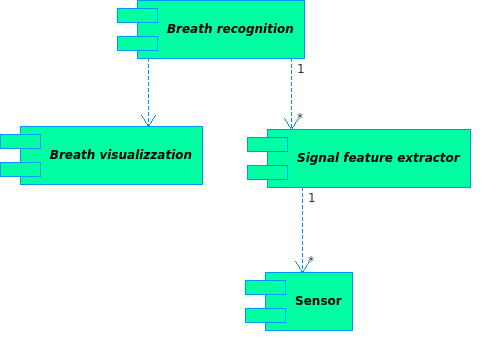
\includegraphics{./metodologiaDiagramma.png}
 % metodologiaDiagramma.png: 504x232 pixel, 96dpi, 13.33x6.14 cm, bb=0 0 378 174
  \caption{Schema generale di un software di riconoscimento della respirazione}
  \label{schemaGeneraleAlg}
\end{figure}


\section{Metodo elementare}
Siamo tentati dal dire che per risolvere il problema \`e sufficiente l'algoritmo \ref{algoritmoElementare}. 
Anche nelle ipotesi che non ci sia alcun rumore ambientale, non abbiamo la certezza che tale algoritmo funzioni per via di altri rumori fisiologici che potrebbero essere rilevati dallo stetoscopio ad esempio suoni cardiovascolari, suoni gastrointestinali e muscolari. 
L'algoritmo tuttavia \`e sottospecificato in quanto ci sono vari gradi di libert\`a: la scelta della soglia e la scelta della dimensione della finestra. 
Dai dati disponibili nella letteratura riguardo i suoni registrati da uno stetoscopio non siamo in grado di dire se possiamo scegliere i parametri dell'algoritmo in modo da farlo funzionare correttamente.
Riteniamo quindi che almeno un primo livello di trattamento del segnale sia necessario per risolvere questo problema. 
Inoltre una implementazione cos\`i banale \`e probabilmente possibile realizzarla ad un livello pi\`u basso ad esempio direttamente nel firmware dello stetoscopio. 

\incmargin{1em}
\restylealgo{boxed}\linesnumbered
\begin{algorithm}
  \dontprintsemicolon
  \SetVline
  % \SetNoline
%   \SetKwData{b}{b}
%   \SetKwData{This}{this}
%   \SetKwData{Up}{up}
  \SetKwFunction{getAverageLocalEnergy}{getAverageLocalEnergy}
  \SetKwFunction{getInstantSoundEnergy}{getSoundEnergy}
  \SetKwFunction{Write}{write}
  \SetKwFunction{Init}{init}
  \SetKwFunction{Clear}{clear}
  \SetKwFunction{Add}{add}
  \SetKwInOut{Input}{input}
  \SetKwInOut{Output}{output}
  \caption{Naive breath detection}

    \Input{A block of sound samples}
%     \Output{A boolean}
    \BlankLine
%     soundEnergyHistoryBuffer.\Clear{}\;
    \ForEach{window $w$ in the input block}{
      instantSoundEnergy $\leftarrow$ w.\getInstantSoundEnergy{}\;
%       averageLocalEnergy $\leftarrow$ soundEnergyHistoryBuffer.\getAverageLocalEnergy{}\;
%       soundEnergyHistoryBuffer.\Write{instantSoundEnergy}\;
% 			//variance = Util.getVariance(soundEnergyHistoryBuffer, averageLocalEnergy);
% 			// final double linearRegression = Util.getLinearRegression(variance);
% 			//final double linearRegression = 1;
% 			//final boolean isABeat = (instantSoundEnergy > (linearRegression * averageLocalEnergy));
      \eIf{instantSoundEnergy $>$ threshold}{
	is a breath;
% 	beatSequence.\Add{true}\;
% 	breathFrequency $\leftarrow$ (breathFrequency + 1) * (59.0 / 60.0)\;
      }{
	is not a breath;
% 	beatSequence.\Add{false}\;
% 	breathFrequency $\leftarrow$ breathFrequency * (59.0 / 60.0)\;
      }
%     \Return beatSequence\;
  }

\label{algoritmoElementare}
\end{algorithm}
\decmargin{1em}





\section{Beat detection}
La soluzione \`e nata dall'osservazione che il respiro ha un certo ritmo e quindi si pu\`o trattare il respiro come se fosse musica. 
La ricerca sul beat detection ha portato ad una serie di algoritmi e metodi per il trattamento di suoni musicali. 
Da una analisi di questi si capisce che possono essere applicati con opportune modifiche anche ai suoni prodotti dal respiro.




\subsection{Scelta dell'algoritmo}

Secondo \cite{Pekonen} ci sono varie propriet\`a da considerare per scegliere un algoritmo di onset detection. 
Ad esempio: 
\begin{itemize}
  \item
    La complessit\`a dell'algoritmo.
  \item
    Le caratteristiche della piattaforma sulla quale ci si aspetta che l'algoritmo venga usato.
  \item
    La presenza o meno di vincoli sul tempo di esecuzione dell'algoritmo. 
  \item
    Il dominio dell'input: 
    \begin{itemize}
      \item
	Se il segnale ha dei beat molto marcati e presenta relativamente poche voci(ad esempio la musica tecno) allora \`e adeguato un metodo nel dominio del tempo.
      \item
	Se il segnale da analizzare \`e complesso, ad esempio nel caso della musica sinfonica nella quale c'\`e una base di strumenti che fanno da accompagnamento e quindi dettano il ritmo della musica e altri gruppi di strumenti pi\`u legati alla melodia, allora conviene usare un metodo basato su informazione di fase nel dominio delle frequenze, in quanto in questo caso i beat sono legati molto al timbro degli strumenti.
    \end{itemize}
  \item
    Se \`e necessaria una localizzazione precisa nel tempo e nelle frequenze allora si possono usare metodi basati sulle wavelet. 
  \item
    Se la complessit\`a computazionale non \`e un problema ed \`e presente un insieme adatto di segnali di allenamento allora si possono usare metodi basati su apprendimento automatico e informazioni statistiche(reti neurali, support vector machine, modelli nascosti di Markov).
\end{itemize}

Ricordiamo che gli algoritmi di onset detection sono progettati per funzionare su brani musicali. 
Questi possono essere un insieme molto complesso di voci musicali. 
Nel nostro caso le ipotesi sull'input sono pi\`u semplici perch\'e possiamo assimilare il suono registrato dallo stetoscopio sul petto ad un brano musicale composto da due voci: i suoni respiratori e i suoni cardiovascolari. 
Anche nel caso dei suoni tracheali abbiamo due voci: i suoni respiratori e i suoni della deglutizione.
Quindi concludiamo che serve un algoritmo che sfrutta sia una analisi nel dominio delle frequenze che una analisi nel dominio del tempo.



\section{Pattern recognition e apprendimento automatico}
Un'altra possibile soluzione attinge al campo del riconoscimento vocale. 
In particolare alcune tecniche di riconoscimento vocale usano dei classificatori che hanno come mattoni di base i fonemi. 
Il suono della respirazione in un certo senso pu\`o essere pensato come un linguaggio parlato nel quale ci sono solo due tipi di fonemi: l'inspirazione e l'espirazione. 
Sia nel linguaggio parlato che nella respirazione \`e anche importante il riconoscimento del silenzio.
  
\subsection{Reti neurali}
Una soluzione di questo tipo si pu\`o implementare attraverso reti neurali. In generale si pu\`o procedere nel modo seguente:
\begin{enumerate}
  \item 
    Prima di tutto bisogna disporre di un database di registrazioni di suoni respiratori. 
  \item
    I suoni possono attraversare una fase di filtraggio nella quale si rimuove il rumore, si riduce eventualmente la frequenza di campionamento e si cerca di eliminare i suoni cardiovascolari.
  \item
    Questi suoni si segmentano in segmenti di due tipi:
    \begin{itemize}
      \item 
	Suoni che contengono respirazione, cio\`e suoni che contengono il suono prodotto dall'espirazione o dall'inspirazione
      \item
	Suoni che contengono pause respiratorie. 
	Per pause respiratorie in questo caso si intende una pausa in generale e quindi non necessariamente una apnea.
    \end{itemize}
  \item
    Per ogni segmento si calcola una sequenza di $S$ propriet\`a statistiche interessanti ad esempio: la media dei valori assoluti dei coefficienti di Fourier in determinate bande di frequenza; la potenza media dei coefficienti wavelet in determinate bande di frequenza; la deviazione standard dei coefficienti in determinate bande di frequenza; il rapporto tra la media dei valori assoluti in bande di frequenza adiacenti. 
  \item
    Si calcola inoltre la quantit\`a $l$ che \`e la media della durata dei segmenti che contengono suoni respiratori.
  \item
    A questo punto si usano i valori calcolati in precedenza per allenare una rete neurale. 
    Una rete neurale \`e un meccanismo per approssimare una funzione quindi per allenare una rete neurale bisogna fornire ad essa delle coppie $(input,\; output)$. 
    In questo caso possiamo usare due neuroni di output e un un numero di neuroni di input pari ad $n$, dove $n$ \`e il numero di propriet\`a dei segmenti di suono calcolate in precedenza. 
    Possiamo costruire un insieme di allenamento nel modo seguente. 
    Se $S$ \`e una sequenza  relativa ad un segmento di respiro allora inseriamo nell'insieme $(S, (1,0))$ mentre se $S$ \`e una sequenza relativa ad un segmento di pausa inseriamo nell'insieme $(S, (0,1))$. 
  \item	
    Dopo che la rete \`e allenata possiamo usarla per classificare un segnale di input. 
    Come prima cosa si divide il segnale in segmenti di dimensione pari ad $l$
  \item
    Si da il segmento in pasto alla rete neurale; questa produce l'output: $(s,p)$. 
  \item
    Se $s$ \`e maggiore di $p$ allora il segmento \`e un suono; altrimenti \`e una pausa.
\end{enumerate}


\section{Clustering}
% DBSCAN nel quale la distanza tra due punti aumenta con la distanza temporale e diminuisce con il quadrato della y
\label{clusteringMetodologia}

Guardando il grafico della forma d'onda del segnale della respirazione, in assenza di forte rumore, nella giusta scala temporale ed entro certi limiti di quantit\`a temporale del segnale, siamo in grado di dividere il grafico in parti regolari e cicliche e di classificarle in: espirazione, inspirazione, pausa. 
Questo approccio metodologico risulta particolarmente chiaro osservando il grafico in figura \ref{grafico}.

\begin{figure}
\centering
 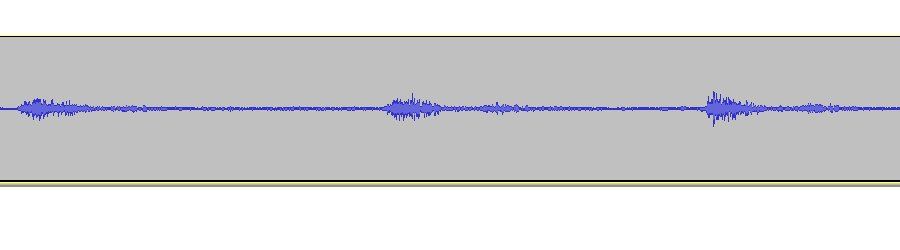
\includegraphics[width=0.7\textwidth]{./metodologiaImage.jpg}
 % metodologiaImage.xcf: 1366x768 pixel, 72dpi, 48.19x27.09 cm, bb=0 0 1366 768
  \label{grafico}
  \caption{Forma d'onda di un segnale che contiene respiro.}
\end{figure}

Tale processo intuitivo si pu\`o inquadrare nel problema pi\`u generale del clustering. Possiamo procedere nel modo seguente:
\begin{enumerate}
  \item 
    Dividere l'input in blocchi di lunghezza ad esempio $20s$ o in ogni caso un valore abbastanza grande da essere sicuri che ci sia un ciclo respiratorio completo. 
  \item
    Trovare un clustering adatto ai dati di input.
  \item
    Un respiro si pu\`o definire come un cluster di inspirazione seguito da un cluster di espirazione seguito da una pausa. Se il clustering contiene una sequenza di respiri allora il soggetto sta respirando altrimenti no.
\end{enumerate}

Rimane il problema di scegliere l'algoritmo di clustering adatto alla nostra situazione. 
Nel nostro caso siamo di fronte ad un problema di clustering nel quale lo spazio del segnale di input \`e bidimensionale. 
Una dimensione \`e il tempo discreto e l'altra dimensione \`e il valore dei campioni. 
Gli algoritmi di clustering impongono di conoscere a priori il numero di cluster oppure un valore di soglia. 
Una possibilit\`a \`e quella di usare l'algoritmo \ref{determinareClusterN} per determinare il pi\`u probabile numero di cluster. 
In seguito confrontiamo questo valore con il numero di fasi che ci dovrebbero essere in media nel blocco di input analizzato. 
Questo dovrebbe andare bene almeno per il primo blocco. 
Per i blocchi successivi possiamo tenere traccia del numero di cluster e confrontare il valore corrente con i valori passati.



\part{Sistema software}
\chapter{Requisiti}



\section{Utenti del sistema software}
Il software pu\`o rientrare in due categorie:
\begin{itemize}
  \item
    La prima categoria si chiama \emph{auscultazione assistita dal calcolatore}, alla quale afferiscono sistemi di supporto alle decisioni cliniche, progettati per aiutare il medico nella diagnosi attraverso i suoni del corpo. 
    In questo caso gli utenti del sistema fanno parte del personale medico-sanitario di una struttura clinica.
  \item
    La seconda categoria \`e il monitoraggio mobile di segnali biomedici. 
    In questo caso gli utenti del sistema possono essere soggetti privi di conoscenze mediche o infermieristiche.
\end{itemize}

% AGGIUNGERE EVENTUALI:
% who is affected either directly or indirectly? 
% who operates the system (normal and maintenance operators)?
% who benefits from the system (functional, political, financial and social beneficiaries)?
% anyone involved in purchasing or procuring the system
% organizations which regulate aspects of the system (financial, safety, and other regulators)
% people or organizations opposed to the system (negative stakeholders; see also Misuse case)
% organizations responsible for systems which interface with the system under design
% those organizations who integrate horizontally with the organization for whom the analyst is designing the system

\begin{center}
  \begin{figure}
  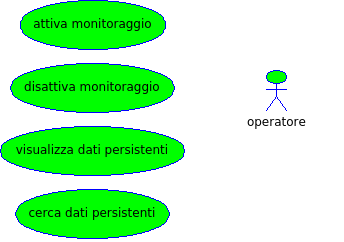
\includegraphics[width=0.5\textwidth,height=0.2\textheight]{./casiDUso.png}
  % casiDUso.png: 339x315 pixel, 96dpi, 8.97x8.33 cm, bb=0 0 254 236
  \caption{Diagramma dei casi d'uso}
  \label{casiDUso}
  \end{figure}
\end{center}



\section{Requisiti funzionali}

% Il software riceve in input il suono registrato sul petto o sulla trachea di soggetti sani o malati e decide la presenza o l'assenza di apnee troppo lunghe in tempo utile. 
% In questo caso il sistema si trova in stato di monitoraggio. 
Il diagramma dei casi d'uso \`e illustrato in figura \ref{casiDUso}:
% Nel seguito ci potremmo riferire alla persona della quale viene monitorato il respiro con il termine \textbf{cliente}. 
I casi d'uso: attiva monitoraggio, visualizza dati persistenti e cerca dati persistenti sono descritti nelle tabelle \ref{casoDUsoMonitoraggio}, \ref{casoDUsoVisualizzaDatiPersistenti} e \ref{casoDUsoCercaDatiPersistenti}. 
% \ref{casoDUsoMonitoraggio}.

   \begin{table}
  \centering
  \begin{tabular}{p{0.17\textwidth} p{0.77\textwidth}}
  \\
  \hline
      Caso d'uso 
    & 
      Attiva monitoraggio
  \\\hline\\
      Attori
    &
      C'\`e un solo attore attivo: un soggetto che intende monitorare il proprio respiro oppure un membro del personale medico sanitario che intende monitorare il respiro di un paziente. Il soggetto del quale si misura il respiro \`e un attore passivo in questo caso d'uso perch\'e in generale esso pu\`o evitare di interagire in modo attivo col sistema stesso. 
  \\
      Precondizioni
    &
      \begin{itemize}
	\item 
	  Lo stetoscopio elettronico \`e stato installato correttamente sul torace del soggetto o sulla trachea del soggetto.
	\item
	  I dispositivi di interfaccia tra lo stetoscopio e il sistema sono configurate correttamente.
      \end{itemize}
  \\
      Sequenza principale degli eventi
    &
      \begin{enumerate}
	\item 
	  L'attore attiva il sistema di monitoraggio attraverso l'interfaccia utente. 
	  In questo passo l'attore specifica se intende memorizzare o meno i dati e in che forma.
	  L'attore pu\`o specificare la soglia di allarme per l'apnea.
	\item
	  Il sistema stabilisce una connessione con lo stetoscopio elettronico. 
	  Se questo passo fallisce allora comincia la sequenza alternativa degli eventi.
	\item	
	  Il sistema passa in fase di monitoraggio.
	\item
	  Se la frequenza di respirazione scende al disotto di una certa soglia critica, il sistema lo segnala attraverso una parte dedicata dell'interfaccia utente, ad esempio un segnale acustico.
      \end{enumerate}      
  \\
      Sequenza alternativa degli eventi
    &
      \begin{enumerate}
	\item 
	  Il sistema segnala un errore appropriato attraverso l'interfaccia utente.
      \end{enumerate}      
  \\
      Postcondizioni
    &
      Il sistema di monitoraggio \`e attivo. 
  \\\\
  \hline
  \end{tabular}
   \caption{Caso d'uso: attiva monitoraggio}
   \label{casoDUsoMonitoraggio}
   \end{table}




   \begin{table}
\centering
  \begin{tabular}{p{0.17\textwidth} p{0.77\textwidth}}
  \\
  \hline
      Caso d'uso 
    & 
      Visualizza dati persistenti
  \\
  \hline\\
      Attori
    &
      C'\`e un solo attore ed \`e l'operatore del sistema. In questo caso d'uso un utente pu\`o consultare i dati relativi ai monitoraggio passati. 
  \\
      Precondizioni
    &
      L'utente conosce le chiavi di accesso ai dati: nome del soggetto e data.
%       \begin{itemize}
% 	\item 
%       \end{itemize}
  \\
      Sequenza principale degli eventi
    &
      \begin{enumerate}
	\item 
	  L'attore inserisce nome del soggetto e/o data nella parte dell'interfaccia utente dedicata alla visualizzazione dei dati persistenti.
	\item
	  Il sistema visualizza i dati relativi alle chiavi inserite, se queste sono corrette. Altrimenti visualizza un messaggio di errore.
% 	\item	
% 	  Se ci sono risultati e l'attore ne seleziona uno, il sistema lo visualizza nella forma specificata dall'interfaccia utente. Un modo per visualizzare i dati potrebbe essere un grafico che ha il tempo sulle ordinate e la frequenza respiratoria sulle ascisse.
      \end{enumerate}      
  \\
      Postcondizioni
    &
      -
  \\\\
  \hline
  \end{tabular}
   \caption{Caso d'uso: visualizza dati persistenti}
   \label{casoDUsoVisualizzaDatiPersistenti}
   \end{table}



   \begin{table}
  \centering
  \begin{tabular}{p{0.17\textwidth} p{0.77\textwidth}}
  \\
  \hline
      Caso d'uso 
    & 
      Cerca dati persistenti
  \\
  \hline\\
      Attori
    &
      Utente del sistema. In questo caso d'uso un utente pu\`o cercare i dati relativi ai monitoraggio passati. Le chiavi di ricerca sono il nome del soggetto e la data.
  \\
      Precondizioni
    &
      -
%       \begin{itemize}
% 	\item 
%       \end{itemize}
  \\
      Sequenza principale degli eventi
    &
      \begin{enumerate}
	\item 
	  L'attore inserisce nome del soggetto e/o data nella parte dell'interfaccia utente dedicata alla ricerca dei dati persistenti.
	\item
	  Il sistema visualizza i risultati della ricerca.
% 	\item	
% 	  Se ci sono risultati e l'attore ne seleziona uno, il sistema lo visualizza nella forma specificata dall'interfaccia utente. Un modo per visualizzare i dati potrebbe essere un grafico che ha il tempo sulle ordinate e la frequenza respiratoria sulle ascisse.
      \end{enumerate}      
  \\
      Postcondizioni
    &
      -
  \\\\
  \hline
  \end{tabular}
   \caption{Caso d'uso: cerca dati persistenti}
   \label{casoDUsoCercaDatiPersistenti}
   \end{table}





\section{Requisiti funzionali opzionali}

Il sistema pu\`o essere arricchito con i requisiti illustrati in figura \ref{opt}. I casi d'uso: visualizza flusso e invia dati sono descritti nella tabelle \ref{visualizzaFlusso} e \ref{inviaDati}.


\begin{figure}
 \centering
 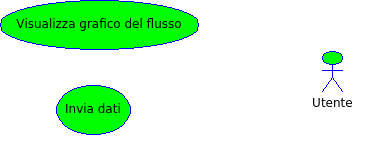
\includegraphics[width=0.4\textwidth]{./opt.png}
 % opt.png: 382x147 pixel, 96dpi, 10.11x3.89 cm, bb=0 0 286 110
  \caption{Diagramma dei casi d'uso opzionali}
\label{opt}
\end{figure}



  \begin{table}
  \centering
  \begin{tabular}{p{0.17\textwidth} p{0.77\textwidth}}
  \\
  \hline
      Caso d'uso 
    & 
      Visualizza flusso
  \\
  \hline\\
      Attori
    &
      Utente del sistema. 
  \\
      Precondizioni
    &
      -
%       \begin{itemize}
% 	\item 
%       \end{itemize}
  \\
      Sequenza principale degli eventi
    &
      In questo caso d'uso il sistema riconosce la localizzazione nel tempo degli eventi inspiratori ed espiratori e visualizza un grafico che ha il tempo sulle ascisse e il valore stimato del flusso sulle ordinate. Nello standard SI un flusso d'aria si misura in litri al secondo. Non \`e necessario stimare il valore oggettivo del flusso ma basta usare valori significativi in modo relativo al flusso massimo e al flusso nullo.
  \\
      Postcondizioni
    &
      -
  \\\\
  \hline
  \end{tabular}
   \caption{Caso d'uso: visualizza flusso}
   \label{visualizzaFlusso}
   \end{table}





   \begin{table}
  \centering
  \begin{tabular}{p{0.17\textwidth} p{0.77\textwidth}}
  \\
  \hline
      Caso d'uso 
    & 
      Invia dati.
  \\
  \hline\\
      Attori
    &
      Utente del sistema. 
  \\
      Precondizioni
    &
      L'utente conosce le chiavi di accesso ai dati e l'URL del personale medico sanitario.
%       \begin{itemize}
% 	\item 
%       \end{itemize}
  \\
      Sequenza principale degli eventi
    &
      \begin{enumerate}
	\item
	  L'utente inserisce le chiavi di accesso ai dati e l'URL del personale medico sanitario nella parte dell'interfaccia utente dedicata a questo caso d'uso.
	\item
	  Il sistema invia i dati e mostra il risultato dell'operazione (successo o fallimento con messaggio d'errore significativo).
      \end{enumerate}
  \\
      Postcondizioni
    &
      -
  \\\\
  \hline
  \end{tabular}
   \caption{Caso d'uso: invia dati}
   \label{inviaDati}
   \end{table}




% \begin{itemize}
%   \item 
%     Distinguere l'inspirazione dall'espirazione e stimare il flusso d'aria.
%   \item	
%     Classificare la respirazione in alcune categorie. Ad esempio distinguere una respirazione normale da una respirazione in presenza di patologie dell'apparato respiratorio e in alcuni casi capire di che malattia si tratta.
% %   \item
% %     Usare un segnale acustico per segnalare condizioni patologiche di emergenza: ad esempio apnea troppo lunga o respirazione di Cheyne-Stokes.
% %   \item
% %     Avere un meccanismo di persistenza dei dati ad esempio un insieme di file in un memoria fissa, un server dedicato o un database remoto o locale.
%   \item
%     Nel caso di home monitoring, offrire la possibilit\`a di inviare i dati ad una struttura sanitaria.
% \end{itemize}

\section{Requisiti non funzionali}

\subsubsection{Sistemi real time}
\cite{RealTime} e \cite{WikiRealTime} danno le seguenti definizioni. Diciamo che un sistema \`e in \emph{tempo reale} o \emph{real time} se la correttezza dell'output dipende anche dal tempo impiegato per calcolarlo. I sistemi real time hanno delle scadenze entro le quali devono dare una risposta. Possiamo classificare i sistemi real time in base alle conseguenze subite dalla mancanza di una risposta entro la scadenza prevista:
\begin{description}
  \item[$hard$]
    Non rispettare una scadenza \`e un errore fatale. 
% Quindi il compito di un sistema real time hard \`e quello di assicurarsi che tutte le scadenza siano rispettate. Nei sistemi real time hard le scadenze devono essere rispettate altrimenti le conseguenze potrebbero essere gravi per le persone o cose di valore. 
  \item[$firm$]
    In questo caso si possono tollerare frequenti mancanze nel rispetto delle scadenze, ma queste mancanze possono degradare la qualit\`a del servizio.
  \item[$soft$]
    Per i sistemi real time soft, l'obiettivo diventa quello di rispettare un certo sottoinsieme di scadenze con lo scopo di ottimizzare alcuni criteri che dipendono dall'applicazione. 
% Il criterio di ottimizzazione particolare dipende dall'applicazione, ad esempio: massimizzare il numero di scadenze soddisfatte o minimizzare il ritardo. 
\end{description}

% In the context of multitasking systems the scheduling policy is normally priority driven (pre-emptive schedulers). Other scheduling algorithms include Earliest Deadline First, which, ignoring the overhead of context switching, is sufficient for system loads of less than 100\%.[2] New overlay scheduling systems, such as an Adaptive Partition Scheduler assist in managing large systems with a mixture of hard real-time and non real-time applications.


% Consider an audio DSP example: if a process requires 2.01 seconds to analyze, synthesize, or process 2.00 seconds of sound, it is not real-time. If it takes 1.99 seconds, it is or can be made into, a real-time DSP process.

\subsubsection{Caratteristiche real time del sistema}

In un sistema real time di elaborazione di segnali digitali, il segnale in input pu\`o essere virtualmente illimitato nel tempo. In realt\`a dei valori che massimizzano la durata del segnale si potrebbero trovare ma sono abbastanza grandi da costringerci ad usare una particolare definizione di scadenze temporali. 
Il ritardo nell'elaborazione deve essere limitato anche se il processo continua per un tempo illimitato. Quindi consideriamo la media del tempo di elaborazione del segnale per campione di segnale in un intervallo di tempo abbastanza piccolo rispetto ai vincoli real time, ad esempio un secondo. Questa media non deve essere maggiore del periodo di campionamento. Questo criterio vale sia che il segnale venga esaminato in blocchi sia che il segnale venga esaminato campione per campione\cite{RTDSPIA}.
In altre parole un sistema real time di elaborazione di un segnale virtualmente illimitato deve avere un tempo di esecuzione per secondo di segnale, minore di un secondo.


La velocit\`a di esecuzione un algoritmo \`e una grandezza data dal rapporto tra la dimensione dell'input e il tempo di esecuzione su di esso.
In questo caso la dimensione dell'input \`e la durata del segnale e non ci interessa la velocit\`a calcolata su tutto il segnale di input ma quella calcolata ad intervalli regolari di dimensione piccola rispetto ai vincoli real time.
Quindi si pu\`o definire la velocit\`a $v$ del processo come la quantit\`a di campioni che ci sono in un secondo di segnale, fratto il tempo impiegato per l'elaborazione di un secondo di segnale. 
In un secondo di segnale ci sono un numero di campioni pari alla frequenza di campionamento del segnale $f_{c} Hz$.
% Siamo abituati a pensare alla velocit\`a come ad una misura di spazio fratto una misura di tempo e quindi pu\`o sembrare controintuitivo misurare la velocit\`a in secondi al secondo ma in questo caso la dimensione dell'input \`e calcolabile in secondi.
Il sistema pu\`o calcolare tale velocit\`a ogni secondo e quindi produrre una sequenza di velocit\`a $v_{1}, v_{2}, \cdots $. 
Una condizione necessaria affinch\'e il sistema si trovi sempre (ogni secondo) in uno stato valido \`e la seguente:
\[
  \forall n.\; v_{n} \geq f_{c}
\]

% Si definisce il ritardo globale relativo al tempo $n$ (calcolato in secondi) come 
% \[
%   r_{g}(n)=f_{c} \cdot n  - 1s \cdot \displaystyle\sum_{i=1}^{n} v_{i} 
% \]
% ed \`e significativo solo se \`e positivo, altrimenti significa che il sistema non ha accumulato ritardo al tempo $n$. Il ritardo globale ha come unit\`a di misura il numero di campioni. Il ritardo $r_{g}$ si traduce in un tempo di ritardo in secondi pari a 
% \[
%   \displaystyle \frac{r_{g}}{f_{c}}
% \]
% nell'ipotesi che il sistema processi il segnale in blocchi di un secondo.

Il sistema in fase di monitoraggio deve segnalare la presenza di apnee troppo lunghe. In particolare consideriamo troppo lunga una apnea di $30$ secondi. Partiamo dall'assunto che le sole scadenze siano quelle relative all'evento apnea troppo lunga e che non rispettare una scadenza significa non dare l'allarme in tempo prima che il soggetto rischi gravi problemi cardiorespiratori. Allora ci troviamo in presenza di un sistema real time hard. Tuttavia i vincoli di tempo per le scadenze sono blandi relativamente ai tempi di esecuzione che si possono prevedere su un calcolatore moderno.

% Una condizione sufficiente affinch\'e il sistema si trovi in uno stato di errore \`e che il ritardo globale superi i $30s \cdot f_{c} Hz$ campioni. 

























\section{Requisiti non funzionali opzionali}
Il software deve funzionare bene anche in presenza di rumore. 



\section{Scelta della soglia di allarme}

La soglia oltre la quale una apnea \`e considerata pericolosa deve essere configurabile.
Il valore soglia deve essere stabilito da personale medico qualificato.
Si pu\`o intuire che una soglia troppo bassa potrebbe degradare la qualit\`a del sonno del soggetto in un modo patogenico o quantomeno in un modo tale da rendere inutile il monitoraggio.
Al contrario una soglia troppo alta espone il soggetto ad un rischio troppo elevato.
Ci si pu\`o aspettare che la soglia di allarme non sia oggettiva ma debba essere personalizzata e che vari con l'et\`a e alcuni parametri fisiologici del soggetto.






\chapter{Architettura}


% Un algoritmo si dice \emph{online} se processa il suo input pezzo dopo pezzo in modo sequenziale, cio\`e nell'ordine nel quale l'input viene dato all'algoritmo. L'algoritmo deve produrre risultati a priori cio\`e anche senza avere a disposizione l'intero input fin dall'inizio. D'altro canto un algoritmo si dice \emph{offline} se pu\`o produrre una risposta anche dopo aver analizzato tutto il suo input. Per sua natura un algoritmo online deve fare delle scelte parziali. 

\section{Componenti}

\begin{figure}
  \centering
  %  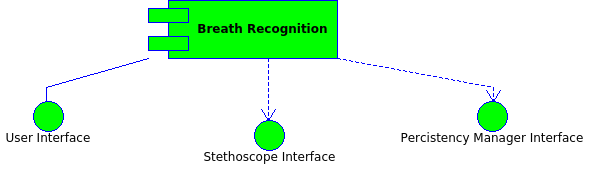
\includegraphics[width=\textwidth,height=0.4\textheight]{./componentdiagram.png}
  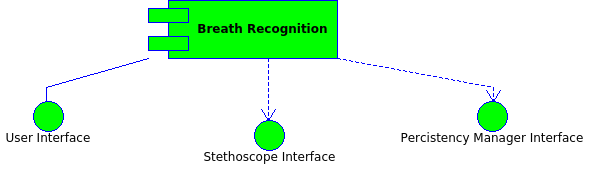
\includegraphics[width=0.8\textwidth]{./componentdiagram.png}
  % componentdiagram.png: 963x508 pixel, 96dpi, 25.48x13.44 cm, bb=0 0 722 381
  \caption{Diagramma delle componenti del sistema}
  \label{componentiSistemaArchitettura}
\end{figure}

Il sistema di monitoraggio ha le componenti illustrate nella figura \ref{componentiSistemaArchitettura}. Discutiamo di ognuna di esse pi\`u in dettaglio nel seguito del capitolo

\subsection{Meccanismi di persistenza}

Il sistema implementa dei meccanismi di persistenza. Un interfaccia minimale di una componente che implementa un meccanismo di persistenza deve offrire le operazioni seguenti:
\begin{itemize}
  \item 
    Aggiungere i dati di nuovo soggetto.
  \item
    Aggiungere una entry di dati di un monitoraggio relativa ad un certo soggetto.
  \item
    Cercare una entry di dati di un monitoraggio a partire dai dati del soggetto e/o dalla data del monitoraggio.
  \item
    Reperire una entry di dati di un monitoraggio a partide da una chiave cercata in precedenza.
\end{itemize}

% Siamo di fronte ad un classico caso di tipo di dato astratto memoria associativa. 
La figura \ref{pppppp} elenca alcuni possibli modi di implementare questo meccanismo di persistenza.


\begin{figure}
  \centering
  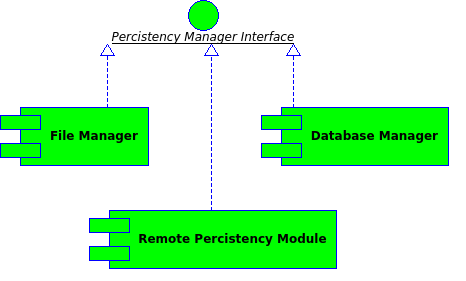
\includegraphics{./persistencyManagerInterface.png}
  % persistencyManagerInterface.png: 466x281 pixel, 96dpi, 12.33x7.43 cm, bb=0 0 349 211
  \caption{Possibili componenti che implementano l'interfaccia con un meccanismo di persistenza}
  \label{pppppp}
\end{figure}

% \begin{figure}
%  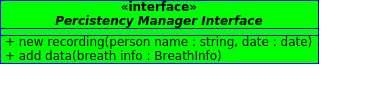
\includegraphics{./persistencyManagerInterfaceOperations.png}
%  % persistencyManagerInterfaceOperations.png: 382x92 pixel, 96dpi, 10.11x2.43 cm, bb=0 0 286 69
%   \label{persistencyManagerInterfaceOperations}
%   \caption{Interfaccia del meccanismo di persistenza}
% \end{figure}

I dati persistenti sono: il nome del sogetto, la data, l'indice di apnea-ipopnea e una sequenza di etichette nell'insieme: respiro o pausa respiratoria. Ogni etichetta corrisponde a $4s$ di segnale. 
% \paragraph{$File\; nella\; memoria\; di\; massa$}
  Il sistema permette di salvare i dati di un monitoraggio sulla memoria di massa del computer sotto forma di file. Vengono usati i meccanismi di serializzazione offerti da Java. La serializzazione di Java permette di memorizzare e leggere uno stream di oggetti Java\cite{javaSerializable}. 
  Per ottimizzare questa operazione, i dati vengono memorizzati prima in un buffer, quando il buffer si riempe vengono scritti sulla memoria di massa. 
  Anche se questa ottimizzazione pu\`o sembrare inutile in quanto tutti i file system moderni sfruttano un meccanismo implicito di buffering, la dimensione di quest'ultimo potrebbe avere un valore predefinito troppo piccolo.


% \paragraph{$Database$}
% Decidere e descrivere cosa come e dove viene memorizzato(tabelle e campi)


% sogetto(
%   nome completo VARCHAR(50),
%   data di nascita DATE,
%   registrazioni: nome di una tabella che contiene tutti i riferimenti alle registrazioni relative a questo soggetto
% )
% 
% persone(
%     id ID,
%     nome completo VARCHAR(50),
%     data di nascita DATE,
%     luogo di nascita VARCHAR(50),
%     luogo di residenza VARCHAR(50),
%     PRIMARY KEY (nome completo, data di nascita, luogo di nascita, id unico)
% )
% 
% registrazioni(
%   soggetto riferimeto a persone
%   
% )






\subsection{Interfaccia con lo stetoscopio}



In generale i sistemi di monitoraggio continuo di parametri fisiologici hanno bisogno di interfacciarsi con i sensori di interesse. 
Questo sistema non \`e una eccezione. 
Riteniamo che una interfaccia minima con lo stetoscopio elettronico sia quella illustrata nella figura \ref{interfacciastetoscopiominima}. Le operazioni illustrate sono:
\begin{description}
  \item[$connect$]
    Inizializza la connessione con il sensore ed allocare eventuali risorse necessarie.
  \item[$disconnect$]
    Terminare la connessione con il sensore e deallocare eventuali risorse.
  \item[$read$]
    Legge $length$ campioni di input e li memorizza nel buffer a partire dall'offset specificato.
  \item[$skip$]
    Tralascia un certo numero di campioni. Puo' essere utile per recuperare in parte un eventuale ritardo globale.
\end{description}



\begin{figure}
\centering
  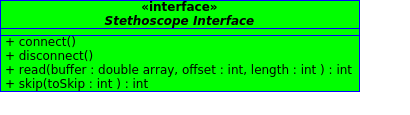
\includegraphics{./stethoscopeInterfaceOperations.png}
% stethoscopeInterfaceOperations.png: 410x115 pixel, 96dpi, 10.85x3.04 cm, bb=0 0 307 86
\caption{Operazioni dell'interfaccia con lo stetoscopio}
\label{interfacciastetoscopiominima}
\end{figure}



Il sistema deve includere almeno una componente che implementa l'interfaccia tra il dispositivo di monitoraggio e il sensore.
Alcune opzioni sono illustrate in figura \ref{componentiinterfacciastetoscopiominima}.

  \begin{figure}
  \centering
 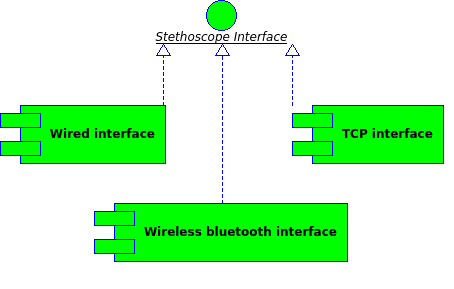
\includegraphics{./stethoscopeInterfaceComponent.png}
 % stethoscopeInterfaceComponent.png: 454x289 pixel, 96dpi, 12.01x7.65 cm, bb=0 0 340 217
  \caption{Possibili componenti che implementano l'interfaccia con lo stetoscopio}
  \label{componentiinterfacciastetoscopiominima}
  \end{figure}

Ci sono appunto vari modi di implementare una connessione tra lo stetoscopio e il dispositivo di monitoraggio. Una scelta che dobbiamo fare riguarda il mezzo di trasmissione del segnale:
\begin{description}
  \item[via cavo]
    In questa modalit\`a spesso \`e necessaria la presenza di personale medico specializzato. Tra gli svantaggi di questa impostazione notiamo: ridotta mobilit\`a del sistema, probabile necessit\`a di alimentazione elettrica dalla rete, rischio di gestione inadeguata di contatti nei cavi.
  \item[senza cavo]
    Una connessione senza fili presenta alcuni vantaggi ad esempio permette al paziente di muoversi pi\`u liberamente e i costi di installazione si possono ridurre.
\end{description}

Riteniamo che per questo sistema sia pi\`u adeguata una connessione senza fili. 

Un'altra scelta riguarda il protocollo di comunicazione, il quale per\`o potrebbe dipendere anche dalla scelta del mezzo di trasmissione.

% Streaming media is multimedia that is constantly received by and presented to an end-user while being delivered by a provider. Its verb form, "to stream", refers to the process of delivering media in this manner; the term refers to the delivery method of the medium rather than the medium itself.
% 
% A client media player can begin playing the data (such as a movie) before the entire file has been transmitted. Distinguishing delivery method from the media distributed applies specifically to telecommunications networks, as most other delivery systems are either inherently streaming (e.g., radio, television) or inherently nonstreaming (e.g., books, video cassettes, audio CDs). 
% For example, in the 1930s, muzak was among the earliest popularly available streaming media; nowadays Internet television is a common form of streamed media. 
% The term "streaming media" can apply to media other than video and audio such as live closed captioning, stock ticker, and real-time text, which are all considered "streaming text". 
% The term "streaming" was first used in the early 1990s as a better description for video on demand on IP networks; at the time such video was usually referred to as "store and forward video",[1] which was misleading nomenclature.
% 
% Live streaming, delivering live over the Internet, involves a camera for the media, an encoder to digitize the content, a media publisher, and a content delivery network to distribute and deliver the content.
% 
% 
% A broadband speed of 2.5 Mbit/s or more is recommended for streaming movies, for example to an Roku, Apple TV, Google TV or a Sony TV Blu-ray Disc Player, 10 Mbit/s for High Definition content.[8]
% 
% 
% 
% Unicast connections require multiple connections from the same streaming server even when it streams the same content
% Streaming media storage size is calculated from the streaming bandwidth and length of the media using the following formula (for a single user and file):
% 
% storage size (in megabytes) = length (in seconds) × bit rate (in bit/s) / (8 × 1024 × 1024)[note 1]
% Real world example:
% 
% One hour of video encoded at 300 kbit/s (this is a typical broadband video as of 2005 and it is usually encoded in a 320 × 240 pixels window size) will be:
% 
% (3,600 s × 300,000 bit/s) / (8×1024×1024) requires around 128 MB of storage.
% If the file is stored on a server for on-demand streaming and this stream is viewed by 1,000 people at the same time using a Unicast protocol, the requirement is:
% 
% 300 kbit/s × 1,000 = 300,000 kbit/s = 300 Mbit/s of bandwidth
% This is equivalent to around 135 GB per hour. Using a multicast protocol the server sends out only a single stream that is common to all users. 
% Therefore such a stream would only use 300 kbit/s of serving bandwidth. See below for more information on these protocols.
% 
% The calculation for live streaming is similar.
% 
% Assumptions: speed at the encoder, is 500 kbit/s.
% 
% If the show lasts for 3 hours with 3,000 viewers, then the calculation is:
% 
% Number of MBs transferred = encoder speed (in bit/s) × number of seconds × number of viewers / (8*1024*1024)
% Number of MBs transferred = 500 x 1024 (bit/s) × 3 × 3,600 ( = 3 hours) × 3,000 (nbr of viewers) / (8*1024*1024) = 1,977,539 MB





Siamo in presenza di un problema la cui modellazione porta naturalmente a pensare ad un pattern architetturale di tipo client server. 
Un server \`e un dispositivo fisico o virtuale che possiede una risorsa da condividere\cite{clientServer}, in questo caso il server \`e lo stetoscopio e la risorsa da condividere \`e il suono che esso registra. Un cliente \`e un dispositivo fisico o virtuale che richiede una certa risorsa ad un server\cite{clientServer}, in questo caso il client \`e il dispositivo di analisi del suono.



\paragraph{bluethoot}
In base alle considerazioni fatte da \cite{BBATMBS}, la teconologia wireless bluethoot si adatta bene al nostro sistema. Il bluethoot permette di stabilire semplici connessioni ad hoc tra dispositivi che hanno a disposizione poca energia elettrica e che sono posti a piccola distanza tra di loro, dove per piccola distanza approssimativamente intendiamo che i dispositivi si trovano nella stessa stanza o anche entro certi limiti in una stessa struttura ospedaliera. I valori precisi di consumi, distanze e velocit\`a di trasmissione variano da dispositivo a dispositivo. Lo stetoscopio elettronico invia continuamente dati al sistema di riconoscimento attraverso il canale bluethoot. I dati inviati dipendono dal particolare stetoscopio ma possiamo aspettarci che questi siano sotto forma di pacchetti di un segnale audio digitale. Suggeriamo quindi di implementare il sistema nel modo illustrato nella figura \ref{blueinterfacciastetoscopiominima}
\begin{figure}
 \centering
 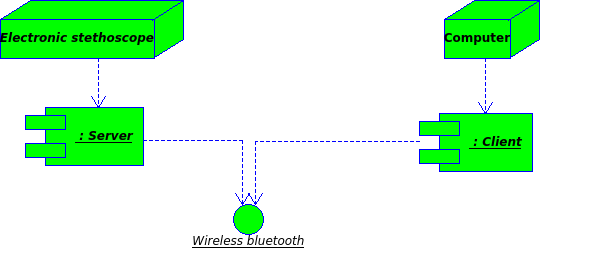
\includegraphics[width=0.9\textwidth]{./deploymentDiagram.png}
 % deploymentDiagram.png: 606x266 pixel, 96dpi, 16.03x7.04 cm, bb=0 0 454 199
  \caption{Architettura del sistema}
  \label{blueinterfacciastetoscopiominima}
\end{figure}


\paragraph{velocit\`a dell'intefaccia}

Supponiamo che il sistema abbia una velocit\`a media di esecuzione di $v_{s}$ campioni di segnale al secondo, e supponiamo che $v$ sia maggiore della frequenza di campionamento e che quindi il sistema riesca ad analizzare un segnale di un secondo in un tempo minore di un secondo. Questa velocit\`a si intende calcolata senza contare il tempo di trasmissione dallo stetoscopio al sistema.

Supponiamo che la velocit\`a di trasmissione dell'interfaccia tra sistema e stetoscopio sia $v_{i}$ bit al secondo e siano $f_{c}$ la frequenza di campionamento del segnale e $size$ la dimensione in bit di un campione di segnale. Allora deve valere
\[
  \displaystyle  \frac{f_{c}}{v_{s}} + \displaystyle \frac{f_{c}}{\left\lfloor\frac{v_{i}}{size}\right\rfloor} \leq 1s
\]
affinch\'e il sistema non accumuli ritardo.













\subsection{Interfaccia utente}



Una interfaccia utente per questo sistema dovrebbe fornire almeno le operazioni elencate nella figura \ref{interfacciautente}.

  \begin{figure}
  \centering
  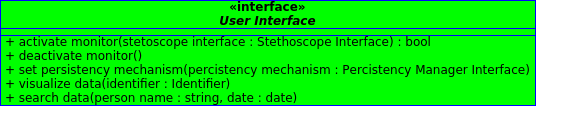
\includegraphics[width=0.8\textwidth]{./userInterfaceOperations.png}
  % userInterfaceOperations.png: 583x138 pixel, 96dpi, 15.42x3.65 cm, bb=0 0 437 103
  \caption{Operazioni dell'interfaccia utente}
  \label{interfacciautente}
  \end{figure}

Sono state implementate due interfacce minimali: 
\begin{description}
  \item[console]
    Un interprete di comandi da console che ha questo aspetto:
    \begin{verbatim}
Breath Monitor Beta version
by Federico Viscomi
type help for a command list

$ help

exit                	exit application             
help                	print this help               
list                	list working directory content
monitor -f filename 	start breath recognition on given file name
stop                	stop current monitoring if any
$ 
    \end{verbatim}

  \item[GUI]
    Una interfaccia grafica basata su Swing \cite{Swing} che offre le stesse funzioni di quella grafica e in pi\`u usa la libreria open source JMathPlot \cite{jmathplot} per disegnare il grafico nel dominio del tempo del segnale. Questo grafico \`e utile solo nella versione iniziale del sistema per motivi di debug. Mentre in una versione successiva del sistema si pu\`o rimpiazzare questo grafico con quello del flusso d'aria. La finestra principale \`e illustrata in figura \ref{finestraprincipale}.
\end{description}

\begin{figure}
 \centering
 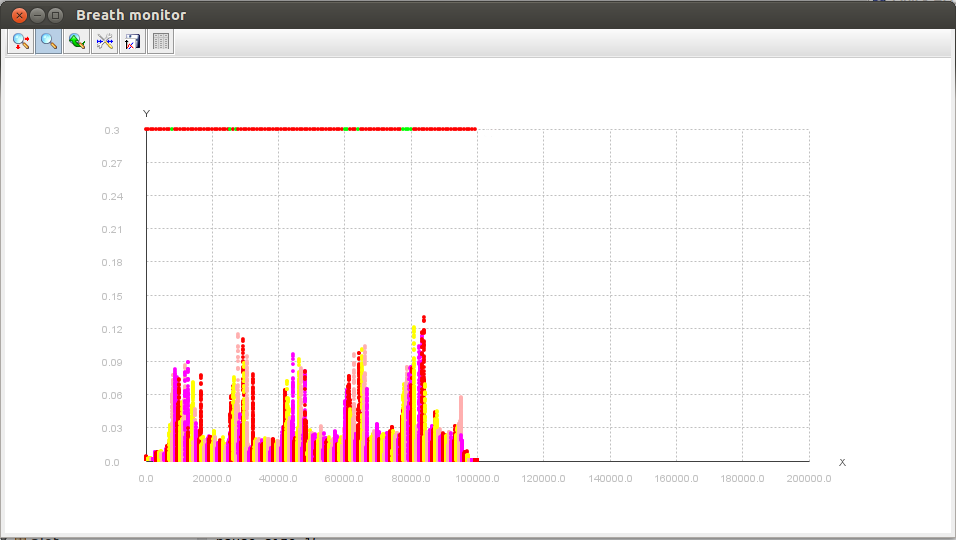
\includegraphics[width=0.8\textwidth]{gui.png}
 % gui.png: 0x0 pixel, 0dpi, 0.00x0.00 cm, bb=
  \label{finestraprincipale}
\end{figure}




\chapter{Implementazione}

\paragraph{Teconologie usate}
    Il sistema \`e stato implementato in Java usando Eclipse come ambiente di sviluppo.
  
  \section{Algoritmo di riconoscimento della respirazione}
    Le fasi di cui si compone l'algoritmo di riconoscimento della respirazione ad un alto livello di astrazione sono illustrate nel diagramma seguente:
    \begin{center}
      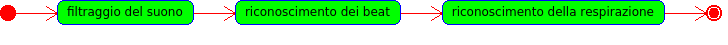
\includegraphics[width=0.9\textwidth,height=0.05\textheight]{./algoritmodiriconoscimentodellarespirazione.png}
    \end{center}

      \paragraph{Filtraggio del segnale audio}
	\begin{wrapfigure}{r}{0.3\textwidth}
	  \begin{center}
	    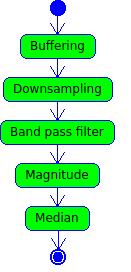
\includegraphics{./filtraggioActivity.png}
	    % onsetActivityDiagram.png: 322x477 pixel, 96dpi, 8.52x12.62 cm, bb=0 0 241 358
	  \end{center}
	  \caption{Diagramma di attivit\`a della fase di filtraggio}
	  \label{filterActivity}
	\end{wrapfigure}
	Il segnale attraversa la successione di fasi a cascata rappresentate nella figura \ref{filterActivity}. 
	Ogni filtro \`e implementato in modo simile a quanto specificato dall'interfaccia $InputStream$ di Java. 
	Siamo davanti ad un tipico caso di design di tipo \emph{pipeline} in quanto l'output di un filtro \`e l'input del filtro successivo(eccetto che per l'ultimo filtro). 
	Il segnale audio, anche nel caso in cui venga letto da un file, \`e trattato come uno \emph{stream} di dati. 
	Pi\`u in dettaglio le fasi di filtraggio sono le seguenti:
      \paragraph{$Buffering/Windowind$}
	Questa fase \`e necessaria in quanto alcuni dei filtri successivi lavorano su blocchi di input e non sul singolo campione. 
	Inoltre la presenza del buffer pu\`o diminuire il tempo totale di elaborazione.
	In questo caso l'input \`e letto da un file quindi non ci sono problemi di overflow.
	Una condizione sufficiente affinch\`e il software rispetti i propri requisiti real time \`e che la velocit\`a di elaborazione sia sempre maggiore di: un secondo di segnale fratto un secondo di tempo di elaborazione. 
      \paragraph{$Downsampling$}
	La sequenza di campionamento viene ridotta con lo scopo di aumentare l'efficienza delle fasi successive dell'algoritmo. 
	Gli spettri di potenza dei suoni respiratori e dei suoni cardiaci hanno frequenze al di sotto dei $500Hz$. 
	Quindi si pu\`o abbassare la frequenza di campionamento a $1000Hz$ in quanto una larghezza di banda di $500Hz$ \`e adeguata a catturare i suoni respiratori\cite{ASPODUOCSS}. 
      \paragraph{$Bandpass filtering$}
	Questo filtro lascia passare solo i suoni che si trovano nella banda di frequenza dai $100$ ai $1500Hz$, il risultato \`e un suono nel quale sono pi\`u facilmente distinguibili i suoni normali della respirazione. 
	Inoltre questo filtro elimina anche alcuni suoni respiratori anormali e parte dei suoni cardiocircolatori.
	Questo filtro \`e implementato grazie alle librerie JSTK reperite all'indirizzo \cite{jstk}. 
	JSTK sta per Java speech toolkit e fornisce tra le altre cose una libreria di tecniche usate per il riconoscimento vocale. 
	La libreria \`e rilasciata secondo la licenza GPLv3.
      \paragraph{$Magnitude filtering$}
	Questo filtro semplicemente prende il valore assoluto del segnale.
      \paragraph{$Median filtergin$}
	Questo \`e un classico filtro a mediana con finestra rettangolare di dimensione $10ms$ e serve per smorzare i suoni accidentali che hanno una intensit\`a relativamente alta rispetto al suono respiratorio e una durata relativamente bassa rispetto alla durata delle fasi respiratorie.

  \section{Algoritmo di beat detection}

    L'algoritmo di beat detection scelto \`e un basato su caratteristiche esplicite del segnale, prese sia dal dominio del tempo che dal dominio delle frequenze. Il thresholding \`e adattativo.
    Scegliamo la dimensione di un blocco in modo tale che contenga $4s$ di campioni dell'input. 
    Mentre scegliamo una dimensione della finestra pari a $10ms$. 
    Sia $w[1...n]$ una finestra all'interno di un blocco di campioni di suono filtrato, definiamo l'energia del suono della finestra $w$ come:
    \[
      \sum_{i=1}^{n} w[i]^{2}
    \]
    definiamo invece l'energia media locale come 
    \[
      \sum_{i=1}^{m} sb[i]^{2}
    \]
    $sb$ \`e un buffer che memorizza gli ultimi valori della media dell'energia locale. 
    Il buffer ha la dimensione adatta ad ospitare i valori relativi ad un blocco.
    % Un beat \`e una grande variazione nell'energia del suono. 
    Un modo semplice per il beat detection \`e la ricerca di picchi nell'energia del suono. 
    In questo modello ci proponiamo di riconoscere le variazioni di energia attraverso il calcolo dell'energia istantanea in una finestra di segnale delle dimensioni di $10ms$ e il confronto di questa con la media dell'energia di un blocco di al pi\`u $4s$ del segnale. 
    Non calcoliamo la media su tutto l'input disponibile perch\'e ci possono essere dei cambiamenti notevoli nel suono della respirazione su un periodo di tempo lungo. 
    Fatte queste premesse possiamo dire che riconosciamo un beat solo quando l'energia istantanea \`e superiore all'energia media. 

    \incmargin{1em}
    \restylealgo{boxed}\linesnumbered
    \begin{algorithm}
      \dontprintsemicolon
      \SetVline
      \SetKwFunction{getAverageLocalEnergy}{getAverageLocalEnergy}
      \SetKwFunction{getInstantSoundEnergy}{getInstantSoundEnergy}
      \SetKwFunction{Write}{write}
      \SetKwFunction{Init}{init}
      \SetKwFunction{Clear}{clear}
      \SetKwFunction{Add}{add}
      \SetKwInOut{Input}{input}
      \SetKwInOut{Output}{output}
      \caption{beat detection}
      \Input{A block of filtered sound samples}
      \Output{A sequence of boolean}
      \BlankLine
      soundEnergyHistoryBuffer.\Clear{}\;
      \ForEach{window $w$ in the input block}{
	instantSoundEnergy $\leftarrow$ w.\getInstantSoundEnergy{}\;
	averageLocalEnergy $\leftarrow$ soundEnergyHistoryBuffer.\getAverageLocalEnergy{}\;
	soundEnergyHistoryBuffer.\Write{instantSoundEnergy}\;
	\eIf{instantSoundEnergy $>$ averageLocalEnergy}{
	  beatSequence.\Add{true}\;
	}{
	  beatSequence.\Add{false}\;
	}
      \Return beatSequence\;
      }
      \label{algBeatDet}
    \end{algorithm}
    \decmargin{1em}



  \section{Riconoscimento delle apnee a rischio}
    La fase di riconoscimento del respiro prende in input le sequenze di booleani date in output dalla fase precedente. 
    Ricordiamo che un elemento della sequenza ha valore di verit\`a vero se corrisponde ad un beat altrimenti vale falso. 
    Questa fase si divide nelle due fasi seguenti.

\paragraph{Clustering}

La prima fase del riconoscimento \`e un \emph{clustering} dei dati della fase precedente. 
In questo contesto un cluster \`e una sequenza di booleani di lunghezza non nota a priori.
Un cluster non deve avere una lunghezza superiore ad una certa soglia ad esempio la lunghezza che corrisponde ad un segnale di $1s$.
% Ci sono solo due tipi di cluster: presenza di suoni respiratori (fase inspiratoria o fase espiratoria) e assenza di suoni respiratori (eventuale apnea). Definiamo il classificatore $C$ nel modo seguente:
% \begin{center}
%   \begin{tabular}{ll}
% 	$C:\tilde{x} \mapsto$ suono
%       &
% 	se $\tilde{x}$ contiene per almeno  $90\%$ beats
%     \\
% 	$C:\tilde{x} \mapsto$ silenzio
%       &
% 	altrimenti
%     \\
%   \end{tabular}
% \end{center}

Usiamo il seguente algoritmo di clustering sequenziale e con cluster sequenziali di lunghezza non nota a priori:
\incmargin{1em}
\restylealgo{boxed}\linesnumbered
\begin{algorithm}
  \dontprintsemicolon
  \SetVline
  % \SetNoline
%   \SetKwData{b}{b}
%   \SetKwData{This}{this}
%   \SetKwData{Up}{up}
  \SetKwFunction{getAverageLocalEnergy}{getAverageLocalEnergy}
  \SetKwFunction{getInstantSoundEnergy}{getInstantSoundEnergy}
  \SetKwFunction{Write}{write}
  \SetKwFunction{Init}{init}
  \SetKwFunction{Clear}{clear}
  \SetKwFunction{Add}{add}
  \SetKwFunction{DDDD}{distance}
  \SetKwInOut{Input}{input}
  \SetKwInOut{Output}{output}
  \caption{Beat clustering}
    \Input{A sequence of boolean $x_{1}, \cdots, x_{n}$}
    \Output{A clustering of the data $C_{1}, \cdots, C_{m}$}
    \BlankLine
    $m\leftarrow 1$\;
    $C_{m}.data \leftarrow \{x_{1}\}$\;
    $C_{m}.type \leftarrow x_{1}$
    \For{$i\leftarrow 2$ \KwTo $n$}{
       \eIf{($\DDDD(x_{i}, C_{m}) > $ threshold) $\vee$ ($C_{m}>maxSize$) $\vee$ $i==n$}{
 	increments $m$\;
	$C_{m}.data \leftarrow \{x_{i}\}$\;
	$C_{m}.type \leftarrow x_{i}$
       }{
 	$C_{m}.data \leftarrow C_{m}.data \cup \{x_{i}\}$\;
       }
  }
\label{clusteringSequenzialeImplementazione}
\end{algorithm}
\decmargin{1em}


La distanza tra un elemento $x_{i}$ e un cluster $C_{m}$ \`e 
% \[
%   distance(x_{i}, C_{m})= 
%   \left|x_{i} -  \displaystyle\frac{\displaystyle\sum_{j\in C_{m}} j}{|C_{m}|}\right|
% \]
\[
distance(x_{i}, C_{m})= 
 \left\{ 
    \begin{array}{ll}
 	\displaystyle\frac{beat\; count}{cluster\; size(C_{m})}
       &
 	se\; x_{i}=false
     \\\\
 	1-\displaystyle\frac{beat\; count}{cluster\; size(C_{m})}
       &
 	se\; x_{i}=true
     \\
     \end{array}
   \right.
\]

La soglia \`e di $0.7$ ed \`e stata scelta in modo empirico.



% 2. FARE UN ESEMPIO DI CLUSTERIZZAZIONE
% dmettere una immagine che mappa una sequenza di beat in una sequenza di cluster!



La fase di cluster serve per correggere eventuali falsi beat della fase precedente, ad esempio un beat che non era causato dal respiro e che non \`e stato eliminato dalla fase di filtraggio oppure serve per aggiungere beat mancanti ad esempio nel caso di una piccola apnea localizzata immediatamente dopo la fase inspiratoria e prima della fase espiratoria.


\paragraph{Riconoscimento delle apnee a rischio}

L'algoritmo considera come pausa respiratoria una sequenza non vuota di cluster $C_{1}, \cdots, C_{n}$ tale che $C_{i}.type=false$ per ogni $i$.
Appena la durata totale della pausa respiratoria supera una soglia critica, il sistema suona una allarme e si mette in attesa che l'allarme venga spenta attraverso un comando apposito dell'interfaccia utente.





\section{Complessit\`a computazionale dell'algoritmo}

Calcolare in modo preciso la complessit\`a asintotica dell'algoritmo \`e difficile perch\`e \`e difficile determinare la complessit\`a del filtro passa banda della libreria JSTK, tuttavia escludendo questa libreria, il resto dell'algoritmo \`e lineare nel numero dei campioni. 
La complessit\`a \`e relativa alla macchina virtuale Java. 











% 


In generale i sistemi di monitoraggio continuo di parametri fisiologici hanno bisogno di interfacciarsi con i sensori di interesse. 
Questo sistema non \`e una eccezione. 
Riteniamo che una interfaccia minima con lo stetoscopio elettronico sia quella illustrata nella figura \ref{interfacciastetoscopiominima}. Le operazioni illustrate sono:
\begin{description}
  \item[$connect$]
    Inizializza la connessione con il sensore ed allocare eventuali risorse necessarie.
  \item[$disconnect$]
    Terminare la connessione con il sensore e deallocare eventuali risorse.
  \item[$read$]
    Legge $length$ campioni di input e li memorizza nel buffer a partire dall'offset specificato.
  \item[$skip$]
    Tralascia un certo numero di campioni. Puo' essere utile per recuperare in parte un eventuale ritardo globale.
\end{description}



\begin{figure}
\centering
  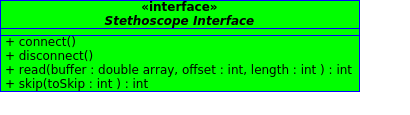
\includegraphics{./stethoscopeInterfaceOperations.png}
% stethoscopeInterfaceOperations.png: 410x115 pixel, 96dpi, 10.85x3.04 cm, bb=0 0 307 86
\caption{Operazioni dell'interfaccia con lo stetoscopio}
\label{interfacciastetoscopiominima}
\end{figure}



Il sistema deve includere almeno una componente che implementa l'interfaccia tra il dispositivo di monitoraggio e il sensore.
Alcune opzioni sono illustrate in figura \ref{componentiinterfacciastetoscopiominima}.

  \begin{figure}
  \centering
 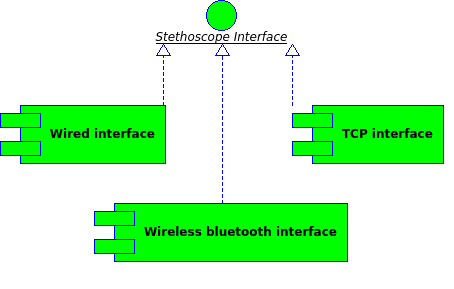
\includegraphics{./stethoscopeInterfaceComponent.png}
 % stethoscopeInterfaceComponent.png: 454x289 pixel, 96dpi, 12.01x7.65 cm, bb=0 0 340 217
  \caption{Possibili componenti che implementano l'interfaccia con lo stetoscopio}
  \label{componentiinterfacciastetoscopiominima}
  \end{figure}

Ci sono appunto vari modi di implementare una connessione tra lo stetoscopio e il dispositivo di monitoraggio. Una scelta che dobbiamo fare riguarda il mezzo di trasmissione del segnale:
\begin{description}
  \item[via cavo]
    In questa modalit\`a spesso \`e necessaria la presenza di personale medico specializzato. Tra gli svantaggi di questa impostazione notiamo: ridotta mobilit\`a del sistema, probabile necessit\`a di alimentazione elettrica dalla rete, rischio di gestione inadeguata di contatti nei cavi.
  \item[senza cavo]
    Una connessione senza fili presenta alcuni vantaggi ad esempio permette al paziente di muoversi pi\`u liberamente e i costi di installazione si possono ridurre.
\end{description}

Riteniamo che per questo sistema sia pi\`u adeguata una connessione senza fili. 

Un'altra scelta riguarda il protocollo di comunicazione, il quale per\`o potrebbe dipendere anche dalla scelta del mezzo di trasmissione.

% Streaming media is multimedia that is constantly received by and presented to an end-user while being delivered by a provider. Its verb form, "to stream", refers to the process of delivering media in this manner; the term refers to the delivery method of the medium rather than the medium itself.
% 
% A client media player can begin playing the data (such as a movie) before the entire file has been transmitted. Distinguishing delivery method from the media distributed applies specifically to telecommunications networks, as most other delivery systems are either inherently streaming (e.g., radio, television) or inherently nonstreaming (e.g., books, video cassettes, audio CDs). 
% For example, in the 1930s, muzak was among the earliest popularly available streaming media; nowadays Internet television is a common form of streamed media. 
% The term "streaming media" can apply to media other than video and audio such as live closed captioning, stock ticker, and real-time text, which are all considered "streaming text". 
% The term "streaming" was first used in the early 1990s as a better description for video on demand on IP networks; at the time such video was usually referred to as "store and forward video",[1] which was misleading nomenclature.
% 
% Live streaming, delivering live over the Internet, involves a camera for the media, an encoder to digitize the content, a media publisher, and a content delivery network to distribute and deliver the content.
% 
% 
% A broadband speed of 2.5 Mbit/s or more is recommended for streaming movies, for example to an Roku, Apple TV, Google TV or a Sony TV Blu-ray Disc Player, 10 Mbit/s for High Definition content.[8]
% 
% 
% 
% Unicast connections require multiple connections from the same streaming server even when it streams the same content
% Streaming media storage size is calculated from the streaming bandwidth and length of the media using the following formula (for a single user and file):
% 
% storage size (in megabytes) = length (in seconds) × bit rate (in bit/s) / (8 × 1024 × 1024)[note 1]
% Real world example:
% 
% One hour of video encoded at 300 kbit/s (this is a typical broadband video as of 2005 and it is usually encoded in a 320 × 240 pixels window size) will be:
% 
% (3,600 s × 300,000 bit/s) / (8×1024×1024) requires around 128 MB of storage.
% If the file is stored on a server for on-demand streaming and this stream is viewed by 1,000 people at the same time using a Unicast protocol, the requirement is:
% 
% 300 kbit/s × 1,000 = 300,000 kbit/s = 300 Mbit/s of bandwidth
% This is equivalent to around 135 GB per hour. Using a multicast protocol the server sends out only a single stream that is common to all users. 
% Therefore such a stream would only use 300 kbit/s of serving bandwidth. See below for more information on these protocols.
% 
% The calculation for live streaming is similar.
% 
% Assumptions: speed at the encoder, is 500 kbit/s.
% 
% If the show lasts for 3 hours with 3,000 viewers, then the calculation is:
% 
% Number of MBs transferred = encoder speed (in bit/s) × number of seconds × number of viewers / (8*1024*1024)
% Number of MBs transferred = 500 x 1024 (bit/s) × 3 × 3,600 ( = 3 hours) × 3,000 (nbr of viewers) / (8*1024*1024) = 1,977,539 MB





Siamo in presenza di un problema la cui modellazione porta naturalmente a pensare ad un pattern architetturale di tipo client server. 
Un server \`e un dispositivo fisico o virtuale che possiede una risorsa da condividere\cite{clientServer}, in questo caso il server \`e lo stetoscopio e la risorsa da condividere \`e il suono che esso registra. Un cliente \`e un dispositivo fisico o virtuale che richiede una certa risorsa ad un server\cite{clientServer}, in questo caso il client \`e il dispositivo di analisi del suono.



\paragraph{bluethoot}
In base alle considerazioni fatte da \cite{BBATMBS}, la teconologia wireless bluethoot si adatta bene al nostro sistema. Il bluethoot permette di stabilire semplici connessioni ad hoc tra dispositivi che hanno a disposizione poca energia elettrica e che sono posti a piccola distanza tra di loro, dove per piccola distanza approssimativamente intendiamo che i dispositivi si trovano nella stessa stanza o anche entro certi limiti in una stessa struttura ospedaliera. I valori precisi di consumi, distanze e velocit\`a di trasmissione variano da dispositivo a dispositivo. Lo stetoscopio elettronico invia continuamente dati al sistema di riconoscimento attraverso il canale bluethoot. I dati inviati dipendono dal particolare stetoscopio ma possiamo aspettarci che questi siano sotto forma di pacchetti di un segnale audio digitale. Suggeriamo quindi di implementare il sistema nel modo illustrato nella figura \ref{blueinterfacciastetoscopiominima}
\begin{figure}
 \centering
 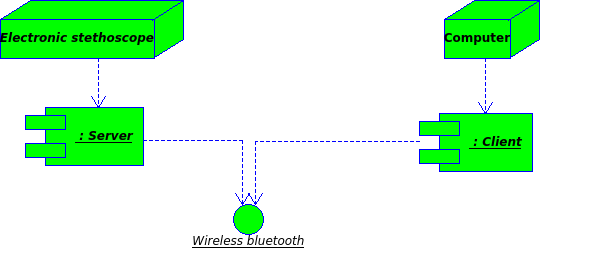
\includegraphics[width=0.9\textwidth]{./deploymentDiagram.png}
 % deploymentDiagram.png: 606x266 pixel, 96dpi, 16.03x7.04 cm, bb=0 0 454 199
  \caption{Architettura del sistema}
  \label{blueinterfacciastetoscopiominima}
\end{figure}


\paragraph{velocit\`a dell'intefaccia}

Supponiamo che il sistema abbia una velocit\`a media di esecuzione di $v_{s}$ campioni di segnale al secondo, e supponiamo che $v$ sia maggiore della frequenza di campionamento e che quindi il sistema riesca ad analizzare un segnale di un secondo in un tempo minore di un secondo. Questa velocit\`a si intende calcolata senza contare il tempo di trasmissione dallo stetoscopio al sistema.

Supponiamo che la velocit\`a di trasmissione dell'interfaccia tra sistema e stetoscopio sia $v_{i}$ bit al secondo e siano $f_{c}$ la frequenza di campionamento del segnale e $size$ la dimensione in bit di un campione di segnale. Allora deve valere
\[
  \displaystyle  \frac{f_{c}}{v_{s}} + \displaystyle \frac{f_{c}}{\left\lfloor\frac{v_{i}}{size}\right\rfloor} \leq 1s
\]
affinch\'e il sistema non accumuli ritardo.










\chapter{Test}
\label{valutazione}

% Per poter realizzare un sistema ottimale per il riconoscimento dell'apnea notturna tramite monitoraggio attraverso uno stetoscopio elettronico bisogna tener conto di alcuni requisiti essenziali del programma.
% Oltre a una verifica del software per assicurarsi che sia corretto e affidabile e altre verifiche come la complessit\`a computazionale e l'utilizzo del processore sono molto importanti dei test valutativi per verificare l'effettiva efficienza del sistema.

\section{Scelta dei casi di test}

Per la scelta dei casi di test usiamo un approccio di tipo black-box e quindi esaminiamo da prima lo spazio dell'input e poi i possibili scenari di uso. 
Il tipo dell'input \`e l'insieme di tutti i possibili segnali audio di durata arbitraria.
Lo spazio dell'input \`e un sottoinsieme del tipo dell'input nel quale rientrano tutti i segnali audio che possono essere ascoltati da uno stetoscopio elettronico posizionato sul petto di un soggetto.

    \`E possibile individuare alcune classi di suoni nello spazio dell'input in base alle sorgenti:
    \begin{center}
    \begin{tikzpicture}
    %   [scale=.8,auto=left,every node/.style={fill=blue!20}]
    [->,>=stealth',shorten >=1pt,auto,node distance=3cm,
      thick,main node/.style={circle,fill=blue!20,draw,font=\sffamily\Large\bfseries}]
      \node (sorgente) at (0,3) {sorgente};
    
      \node (interna) at (4,1.5) {interna al corpo};
      \node (esterna) at (4,4) {esterna al corpo};
    
      \node (n1n1n1) at (9,0) {respiratoria};
      \node (n1n1n2) at (9,0.5) {muscolare};
      \node (n1n1n3) at (9,1) {gastrointestinale};
      \node (n1n1n4) at (9,1.5) {deglutitoria};
      \node (n1n1n5) at (9,2) {vocale};
      \node (n1n1n6) at (9,2.5) {cardiocircolatoria};
    
      \node (n2n1n3) at (9,3.5) {$\vdots$};
      \node (n2n1n2) at (9,4) {voci di persone};
      \node (n2n1n1) at (9,4.5) {traffico veicolare};
      
    
      \foreach \from/\to in {
	  sorgente/interna,sorgente/esterna,
	  interna/n1n1n1,interna/n1n1n2,interna/n1n1n3,interna/n1n1n4,interna/n1n1n5,interna/n1n1n6,
	  esterna/n2n1n1,esterna/n2n1n2,esterna/n2n1n3}
	\draw (\from) -- (\to);
    
    \end{tikzpicture}
    \end{center}


Alcuni casi di test ci vengono dati dai possibili valori che pu\`o avere l'input in uno scenario di uso reale del software. Ad esempio alcuni casi di test possono avere come input:
\begin{itemize}
  \item
    Un file audio abbastanza lungo da simulare un monitoraggio del sonno reale. Lo scopo di un caso d'uso con questo input \`e la valutazione della velocit\`a a lungo termine dell'algoritmo.
  \item
    Dei suoni respiratori sovrapposti a rumore di vari tipo ed intensit\`a. Lo scopo di un caso d'uso con questo input \`e la valutazione della tolleranza al rumore.
  \item
    Suoni respiratori senza rumore. Lo scopo di un caso d'uso con questo input \`e la valutazione del funzionamento del software in uno scenario ideale.
  \item
    Un file audio contenente solo rumore. Questo caso di test serve per capire se il software pu\`o rilevare la presenza di respiro in suoni che non contengono alcun respiro. In uno scenario di uso reale corretto questo caso non si verifica ma \`e comunque interessante.
  \item
    Un file con una frequenza di campionamento molto elevata. Questo caso di test rientra nella categoria stress test. Ci aspettiamo che il sistema si comporti bene se ha un input file con una frequenza di campionamento molto elevata grazie al filtro di sottocampionamento.
  \item
    Un file contenente suoni respiratori sovrapposti a forti suoni cardiaci. 
  \item
    Un file respiratorio contente una apnea pi\`u lunga della soglia massima.
\end{itemize}

Per creare dei casi che valutano la resistenza al rumore si pu\`o procedere nel modo illustrato nella figura \ref{mix} e cio\`e:
\begin{enumerate}
  \item 
    Scegliere una file contenente una sorgente di rumore e scegliere una intensit\`a della sorgente di rumore.
  \item
    Filtrare il file di rumore in base ad un certo modello acustico del corpo. Cio\`e cercare di prevedere cosa lo stetoscopio sente se \`e presente la sorgente di rumore scelta. Questo modello acustico \`e necessariamente un modello approssimato. In una prima fase elementare di modellazione possiamo usare un semplice filtro attenuatore e supporre che il rumore sia di tipo additivo.
  \item
    Scegliere un file contente un respiro.
  \item
    Fare un mix dei file.
\end{enumerate}


\begin{center}
\begin{figure}
\centering
\begin{tikzpicture}[scale=2,->,>=stealth',shorten >=1pt,auto, thick,nodes={draw, ultra thick, fill=none}]
      
      \node[draw=none] (respiro) at (0,1) {respiro};
      \node[draw=none] (rumore) at (0,0) {rumore};

      \node[rectangle] (attenuatore) at (2,0) {filtro attenuatore};
      \node[rectangle] (somma) at (2,1) {+};

      \node[draw=none] (output) at (4,1) {output};



  \foreach \from/\to in {respiro/somma, rumore/attenuatore, attenuatore/somma, somma/output}
     \draw (\from) -- (\to);

\end{tikzpicture}
  \caption{Processo di aggiunta del rumore}
\label{mix}
\end{figure}
\end{center}



Arriva in nostro aiuto il software open source Audacity \cite{audacity} il quale offre una vasta gamma di funzioni di trattamento dell'audio digitale. Quelle utili per i casi di test sono: 
\begin{itemize}
  \item
    Aggiungere rumore di vari tipi (bianco, rosa e marrone) e con varia intensit\`a.
  \item
    Aggiungere segmenti di silenzio di lunghezza a scelta nei file audio e quindi simulare la presenza di una apnea lunga.
  \item
    Concatenare file audio. Questa funzione \`e utile perch\'e i file audio che abbiamo a disposizione reperiti da \cite{SoundRepositories} sono di lunghezza troppo breve (minore di $15s$).
  \item
    Applicare filtri di vario tipo tra i quali un filtro attenuatore.
\end{itemize}


In generale possiamo creare un caso di test attraverso la concatenazione di segmenti di file audio. Ogni segmento contiene una pausa respiratoria sovrapposta ad un rumore oppure un respiro sovrapposto ad un rumore. La tabella seguente riassume le propriet\`a di un segmento di base:
\begin{center}
  \begin{table}[!h]
    \centering
    \begin{tabular}{p{0.15\textwidth} | p{0.5\textwidth} l}
      \hline
	  contenuto
	& 
	  tipo o sorgente
	& 
	  itensit\`a
      \\\hline\\
	  respiro
	& 
	  [normale anormale misto, bronchiale vescicolare, continuo discontinuo, ronchi wheeze stridor crackles squawks]
	& 
	  [0-10]
      \\
	  rumori
	& 
	  [bianco rosa marrone, interno esterno, gastrointestinale deglutitorio vocale, ecc..]
	& 
	  [0-10]
      \\
	  pausa respiratoria
	& 
	  -
	& 
	  -
      \\\hline
    \end{tabular}
    \caption{Propriet\`a di un segmento di base.}
    \label{segmentodibase}
  \end{table}
\end{center}


Non abbiamo a disposizione alcuno stetoscopio per\`o usiamo le registrazioni reperite da \cite{SoundRepositories} e partiamo da queste per creare alcuni casi di test.
Purtroppo le fonti non riportano i dettagli di come sono stati registrati i suoni. 


\section{Valutazione dell'output}
\label{valutareOutput}
\paragraph{Valutare la localizzazione delle fasi respiratorie.}
Se si vuole valutare un algoritmo che localizza nel tempo le fasi respiratorie allora pensiamo ad un suono respiratorio come ad una sequenza di cicli respiratori e ad  un ciclo respiratorio come una fase di inspirazione seguita da una fase di espirazione seguita da una pausa. 

Quindi lo spazio di input \`e classificabile in sequenze crescenti di numeri razionali che indicano la posizione temporale dell'inizio di ciascuna fase. L'output dell'algoritmo sar\`a una sequenza di numeri razionali che indicano la localizzazione temporale dell'inizio di ciascuna fase. 
Definiamo la differenza tra l'output e il descrittore della classe di cui fa parte l'input come la sequenza dei valori assoluti delle differenze delle singole componenti. 
La qualit\`a dell'algoritmo si pu\`o misurare in termini di qualche propriet\`a statistica di questa differenza, ad esempio la media.


\paragraph{Valutare la localizzazione delle apnee.}
Se si vuole valutare un algoritmo che riconosce la presenza di una apnea allora possiamo classificare lo spazio dell'input in sequenze di coppie di numeri razionali tali che ogni coppia contiene il tempo di inizio e il tempo di fine di una apnea. In tal caso anche l'output sar\`a una sequenza di coppie di numeri razionali. 
Supponiamo che in input ci sia una apnea che comincia al tempo $s_{in}$ e finisce al tempo $f_{in}$. Si possono verificare vari casi:
\begin{itemize}
  \item
    Esiste un solo intervallo temporale di output $(s_{out}, f_{out})$ che interseca l'intervallo $(s_{in}, f_{in})$. Allora definiamo l'errore di riconoscimento dell'evento $(s_{in}, f_{in})$ come 
    \[
      |s_{out}-s_{in}| + |f_{out}-f_{in}|
    \]
    e diciamo che l'evento $(s_{in}, f_{in})$ \`e un \emph{vero positivo} cio\`e un evento riconosciuto in modo corretto.
  \item
    Se non ci sono intervalli temporali di output che intersecano $(s_{in}, f_{in})$ allora diciamo che questo evento \`e un \emph{falso positivo}. I falsi positivi sono gli errori pi\`u gravi e che quindi incidono maggiormente nella valutazione di un algoritmo.
  \item
    Se ci sono pi\`u intervalli temporali di output che intersecano $(s_{in}, f_{in})$ allora la scelta di come valutare la qualit\`a dell'algoritmo \`e arbitraria e pu\`o essere ad esempio 
    \[
      |min(s_{out})-s_{in}| + |max(f_{out})-f_{in}|
    \]
\end{itemize}
Rimane il caso in cui l'algoritmo produce un output $(s_{out}, f_{out})$ ma non abbiamo nessun intervallo di input che lo interseca. 
In tal caso parliamo di \emph{falso negativo} ed \`e un errore meno grave di un falso positivo. 

\paragraph{Valutare la localizzazione delle apnee a rischio.}
Se si vuole valutare un algoritmo che riconosce la presenza di una apnea troppo lunga allora possiamo classificare lo spazio dell'input come nel caso precedente ma l'analisi che ne risulta \`e diversa.
Supponiamo che in input ci sia una apnea troppo lunga (cio\`e maggiore di una certa soglia $S$ di sicurezza) che comincia al tempo $s_{in}$ e finisce al tempo $f_{in}$. Si possono verificare vari casi:
\begin{itemize}
  \item
    C'\`e almeno un intervallo temporale di output $(s_{out}, f_{out})$ tale che 
    \begin{itemize}
      \item 
	$(s_{out}, f_{out})$ interseca $(s_{in}, f_{in})$
      \item
	$s_{out} + S \leq s_{in} + S + T$ dove $T$ \`e una soglia di tolleranza dell'errore.
      \item
	$f_{out}-s_{out}>S$
    \end{itemize}
    In tal caso diciamo che l'evento $(s_{in}, f_{in})$ \`e un \emph{vero positivo} cio\`e un evento riconosciuto in modo corretto.
  \item
    Se non ci sono intervalli temporali di output con le propriet\`a elencate al punto precedente allora diciamo che l'evento $(s_{in}, f_{in})$ \`e un \emph{falso positivo}.
\end{itemize}
Rimane il caso in cui l'algoritmo produce in output un intervallo $(s_{out}, f_{out})$ di lunghezza maggiore della soglia di sicurezza ma non abbiamo nessun intervallo di input che lo interseca e che ha durata maggiore della soglia di sicurezza. 
In tal caso abbiamo un \emph{falso negativo}. 
Si pu\`o anche definire cosa intendiamo per \emph{vero negativo} e cio\`e una mancanza di apnea troppo lunga che l'algoritmo non classifica come apnea troppo lunga. 
Tuttavia questa definizione non si applica in modo elegante alle premesse fatte in questo paragrafo. 
La tabella seguente ricapitola i vari casi:
\begin{center}
    \begin{tabular}{|l|ll|}
      \hline
      \emph{evento: apnea troppo lunga} & evento presente & evento assente \\
      \hline
      evento riconosciuto        & \bf{vero positivo}   & \bf{falso negativo} \\
      evento non riconosciuto    & \bf{falso positivo}  & \bf{vero negativo}  \\
      \hline
    \end{tabular}
\end{center}

Si pu\`o capire facilmente quale significato abbia la classificazione precedente, se si immagina uno scenario di uso del software.


\begin{bf}Vero positivo.\end{bf}
  Il soggetto ha una apnea nel sonno troppo lunga e il sistema suona l'allarme. Il soggetto si sveglia, spegne l'allarme e torna a dormire sano e salvo (si spera).


\begin{bf}Vero negativo.\end{bf}
  Il soggetto non ha una apnea nel sonno troppo lunga e il sistema non suona l'allarme. Questo caso \`e auspicabile. Maggiore \`e la frequenza di questi casi, maggiore \`e la qualit\`a del sonno del soggetto.


\begin{bf}Falso positivo.\end{bf}
  Il soggetto ha una apnea nel sonno troppo lunga e il sistema non suona l'allarme. Questo caso \`e rischioso per la salute del paziente.


\begin{bf}Falso negativo.\end{bf}
  Il soggetto non ha una apnea nel sonno troppo lunga e il sistema suona l'allarme. Il soggetto si sveglia, spegne l'allarme e torna a dormire. Non ha modo di capire se si \`e verificato un vero positivo o un falso negativo (quindi non impreca contro gli sviluppatori del software).
    I falsi negativi degradano la qualit\`a del sonno del soggetto ma non sono un rischio grave per la salute quanto i falsi positivi.
    Tuttavia se il degrado nella qualit\`a del sonno \`e eccessivo potrebbe causare danni psicofisici al soggetto che eventualmente superano quelli causati dalla sindrome da apnea del sonno.
    Quindi \`e anche importante che il sistema non generi molti falsi negativi.




\section{Test}
\begin{frame}
  \frametitle{Creare i casi di test}
  \begin{itemize}
    \item
      Approccio black box. 
    \item
      Analisi dello spazio dell'input e degli scenari di uso reale.
    \item
      Concatenazione di segmenti di file audio:
% 
% Per la scelta dei casi di test usiamo un approccio di tipo black-box e quindi esaminiamo da prima lo spazio dell'input e poi i possibili scenari di uso. 
% Il tipo dell'input \`e l'insieme di tutti i possibili segnali audio di durata arbitraria.
% Lo spazio dell'input \`e un sottoinsieme del tipo dell'input nel quale rientrano tutti i segnali audio che possono essere ascoltati da uno stetoscopio elettronico posizionato sul petto di un soggetto.
% 
%     \`E possibile individuare alcune classi di suoni nello spazio dell'input in base alle sorgenti:
%     \begin{center}
%     \begin{tikzpicture}
%     %   [scale=.8,auto=left,every node/.style={fill=blue!20}]
%     [->,>=stealth',shorten >=1pt,auto,node distance=3cm,
%       thick,main node/.style={circle,fill=blue!20,draw,font=\sffamily\Large\bfseries}]
%       \node (sorgente) at (0,3) {sorgente};
%     
%       \node (interna) at (4,1.5) {interna al corpo};
%       \node (esterna) at (4,4) {esterna al corpo};
%     
%       \node (n1n1n1) at (9,0) {respiratoria};
%       \node (n1n1n2) at (9,0.5) {muscolare};
%       \node (n1n1n3) at (9,1) {gastrointestinale};
%       \node (n1n1n4) at (9,1.5) {deglutitoria};
%       \node (n1n1n5) at (9,2) {vocale};
%       \node (n1n1n6) at (9,2.5) {cardiocircolatoria};
%     
%       \node (n2n1n3) at (9,3.5) {$\vdots$};
%       \node (n2n1n2) at (9,4) {voci di persone};
%       \node (n2n1n1) at (9,4.5) {traffico veicolare};
%       
%     
%       \foreach \from/\to in {
% 	  sorgente/interna,sorgente/esterna,
% 	  interna/n1n1n1,interna/n1n1n2,interna/n1n1n3,interna/n1n1n4,interna/n1n1n5,interna/n1n1n6,
% 	  esterna/n2n1n1,esterna/n2n1n2,esterna/n2n1n3}
% 	\draw (\from) -- (\to);
%     
%     \end{tikzpicture}
%     \end{center}
% 
% 
% Alcuni casi di test ci vengono dati dai possibili valori che pu\`o avere l'input in uno scenario di uso reale del software. Ad esempio alcuni casi di test possono avere come input:
% \begin{itemize}
%   \item
%     Un file audio abbastanza lungo da simulare un monitoraggio del sonno reale. Lo scopo di un caso d'uso con questo input \`e la valutazione della velocit\`a a lungo termine dell'algoritmo.
%   \item
%     Dei suoni respiratori sovrapposti a rumore di vari tipo ed intensit\`a. Lo scopo di un caso d'uso con questo input \`e la valutazione della tolleranza al rumore.
%   \item
%     Suoni respiratori senza rumore. Lo scopo di un caso d'uso con questo input \`e la valutazione del funzionamento del software in uno scenario ideale.
%   \item
%     Un file audio contenente solo rumore. Questo caso di test serve per capire se il software pu\`o rilevare la presenza di respiro in suoni che non contengono alcun respiro. In uno scenario di uso reale corretto questo caso non si verifica ma \`e comunque interessante.
%   \item
%     Un file con una frequenza di campionamento molto elevata. Questo caso di test rientra nella categoria stress test. Ci aspettiamo che il sistema si comporti bene se ha un input file con una frequenza di campionamento molto elevata grazie al filtro di sottocampionamento.
%   \item
%     Un file contenente suoni respiratori sovrapposti a forti suoni cardiaci. 
%   \item
%     Un file respiratorio contente una apnea pi\`u lunga della soglia massima.
% \end{itemize}
% 
% Per creare dei casi che valutano la resistenza al rumore si pu\`o procedere nel modo illustrato nella figura \ref{mix} e cio\`e:
% \begin{enumerate}
%   \item 
%     Scegliere una file contenente una sorgente di rumore e scegliere una intensit\`a della sorgente di rumore.
%   \item
%     Filtrare il file di rumore in base ad un certo modello acustico del corpo. Cio\`e cercare di prevedere cosa lo stetoscopio sente se \`e presente la sorgente di rumore scelta. Questo modello acustico \`e necessariamente un modello approssimato. In una prima fase elementare di modellazione possiamo usare un semplice filtro attenuatore e supporre che il rumore sia di tipo additivo.
%   \item
%     Scegliere un file contente un respiro.
%   \item
%     Fare un mix dei file.
% \end{enumerate}
% 
% 
% \begin{center}
% \begin{figure}
% \centering
% \begin{tikzpicture}[scale=2,->,>=stealth',shorten >=1pt,auto, thick,nodes={draw, ultra thick, fill=none}]
%       
%       \node[draw=none] (respiro) at (0,1) {respiro};
%       \node[draw=none] (rumore) at (0,0) {rumore};
% 
%       \node[rectangle] (attenuatore) at (2,0) {filtro attenuatore};
%       \node[rectangle] (somma) at (2,1) {+};
% 
%       \node[draw=none] (output) at (4,1) {output};
% 
% 
% 
%   \foreach \from/\to in {respiro/somma, rumore/attenuatore, attenuatore/somma, somma/output}
%      \draw (\from) -- (\to);
% 
% \end{tikzpicture}
%   \caption{Processo di aggiunta del rumore}
% \label{mix}
% \end{figure}
% \end{center}
% 
% 
% 
% Arriva in nostro aiuto il software open source Audacity \cite{audacity} il quale offre una vasta gamma di funzioni di trattamento dell'audio digitale. Quelle utili per i casi di test sono: 
% \begin{itemize}
%   \item
%     Aggiungere rumore di vari tipi (bianco, rosa e marrone) e con varia intensit\`a.
%   \item
%     Aggiungere segmenti di silenzio di lunghezza a scelta nei file audio e quindi simulare la presenza di una apnea lunga.
%   \item
%     Concatenare file audio. Questa funzione \`e utile perch\'e i file audio che abbiamo a disposizione reperiti da \cite{SoundRepositories} sono di lunghezza troppo breve (minore di $15s$).
%   \item
%     Applicare filtri di vario tipo tra i quali un filtro attenuatore.
% \end{itemize}
% 
% 

 
 \begin{center}
   \begin{table}[!h]
     \centering
     \begin{tabular}{p{0.15\textwidth} | p{0.5\textwidth} l}
       \hline
 	  contenuto
 	& 
 	  tipo o sorgente
 	& 
 	  itensit\`a
       \\\hline\\
 	  respiro
 	& 
%  	  [normale anormale misto, bronchiale vescicolare, continuo discontinuo, ronchi wheeze stridor crackles squawks]
	  [normale, anormale, misto, bronchiale, vescicolare, continuo, ...]
 	& 
 	  [0-10]
       \\
 	  rumori
 	& 
 	  [bianco, rosa, interno, esterno, gastrointestinale, ...]
 	& 
 	  [0-10]
       \\
 	  pausa respiratoria
 	& 
 	  -
 	& 
 	  -
       \\\hline
     \end{tabular}
   \end{table}
 \end{center}
  \end{itemize} 
% 
% Non abbiamo a disposizione alcuno stetoscopio per\`o usiamo le registrazioni reperite da \cite{SoundRepositories} e partiamo da queste per creare alcuni casi di test.
% Purtroppo le fonti non riportano i dettagli di come sono stati registrati i suoni. 
% 

\end{frame}


\begin{frame}
  \frametitle{Valutazione dell'output}
  \framesubtitle{Localizzazione delle apnee a rischio}
% 
% \section{Valutazione dell'output}
% \label{valutareOutput}
% \paragraph{Valutare la localizzazione delle fasi respiratorie.}
% Se si vuole valutare un algoritmo che localizza nel tempo le fasi respiratorie allora pensiamo ad un suono respiratorio come ad una sequenza di cicli respiratori e ad  un ciclo respiratorio come una fase di inspirazione seguita da una fase di espirazione seguita da una pausa. 
% 
\begin{itemize}
  \item 
    Classificazione dello spazio dell'input: sequenze di intervalli di numeri razionali che indicano la posizione temporale di ciascuna fase di apnea.
  \item
    Classificazione dell'output rispetto alla classe di input:
% Quindi lo spazio di input \`e classificabile in sequenze crescenti di numeri razionali che indicano la posizione temporale dell'inizio di ciascuna fase. L'output dell'algoritmo sar\`a una sequenza di numeri razionali che indicano la localizzazione temporale dell'inizio di ciascuna fase. 
% Definiamo la differenza tra l'output e il descrittore della classe di cui fa parte l'input come la sequenza dei valori assoluti delle differenze delle singole componenti. 
% La qualit\`a dell'algoritmo si pu\`o misurare in termini di qualche propriet\`a statistica di questa differenza, ad esempio la media.
% 
% 
% \paragraph{Valutare la localizzazione delle apnee.}
% Se si vuole valutare un algoritmo che riconosce la presenza di una apnea allora possiamo classificare lo spazio dell'input in sequenze di coppie di numeri razionali tali che ogni coppia contiene il tempo di inizio e il tempo di fine di una apnea. In tal caso anche l'output sar\`a una sequenza di coppie di numeri razionali. 
% Supponiamo che in input ci sia una apnea che comincia al tempo $s_{in}$ e finisce al tempo $f_{in}$. Si possono verificare vari casi:
% \begin{itemize}
%   \item
%     Esiste un solo intervallo temporale di output $(s_{out}, f_{out})$ che interseca l'intervallo $(s_{in}, f_{in})$. Allora definiamo l'errore di riconoscimento dell'evento $(s_{in}, f_{in})$ come 
%     \[
%       |s_{out}-s_{in}| + |f_{out}-f_{in}|
%     \]
%     e diciamo che l'evento $(s_{in}, f_{in})$ \`e un \emph{vero positivo} cio\`e un evento riconosciuto in modo corretto.
%   \item
%     Se non ci sono intervalli temporali di output che intersecano $(s_{in}, f_{in})$ allora diciamo che questo evento \`e un \emph{falso positivo}. I falsi positivi sono gli errori pi\`u gravi e che quindi incidono maggiormente nella valutazione di un algoritmo.
%   \item
%     Se ci sono pi\`u intervalli temporali di output che intersecano $(s_{in}, f_{in})$ allora la scelta di come valutare la qualit\`a dell'algoritmo \`e arbitraria e pu\`o essere ad esempio 
%     \[
%       |min(s_{out})-s_{in}| + |max(f_{out})-f_{in}|
%     \]
% \end{itemize}
% Rimane il caso in cui l'algoritmo produce un output $(s_{out}, f_{out})$ ma non abbiamo nessun intervallo di input che lo interseca. 
% In tal caso parliamo di \emph{falso negativo} ed \`e un errore meno grave di un falso positivo. 
% 
% \paragraph{Valutare la localizzazione delle apnee a rischio.}
% Se si vuole valutare un algoritmo che riconosce la presenza di una apnea troppo lunga allora possiamo classificare lo spazio dell'input come nel caso precedente ma l'analisi che ne risulta \`e diversa.
% Supponiamo che in input ci sia una apnea troppo lunga (cio\`e maggiore di una certa soglia $S$ di sicurezza) che comincia al tempo $s_{in}$ e finisce al tempo $f_{in}$. Si possono verificare vari casi:
% \begin{itemize}
%   \item
%     C'\`e almeno un intervallo temporale di output $(s_{out}, f_{out})$ tale che 
%     \begin{itemize}
%       \item 
% 	$(s_{out}, f_{out})$ interseca $(s_{in}, f_{in})$
%       \item
% 	$s_{out} + S \leq s_{in} + S + T$ dove $T$ \`e una soglia di tolleranza dell'errore.
%       \item
% 	$f_{out}-s_{out}>S$
%     \end{itemize}
%     In tal caso diciamo che l'evento $(s_{in}, f_{in})$ \`e un \emph{vero positivo} cio\`e un evento riconosciuto in modo corretto.
%   \item
%     Se non ci sono intervalli temporali di output con le propriet\`a elencate al punto precedente allora diciamo che l'evento $(s_{in}, f_{in})$ \`e un \emph{falso positivo}.
% \end{itemize}
% Rimane il caso in cui l'algoritmo produce in output un intervallo $(s_{out}, f_{out})$ di lunghezza maggiore della soglia di sicurezza ma non abbiamo nessun intervallo di input che lo interseca e che ha durata maggiore della soglia di sicurezza. 
% In tal caso abbiamo un \emph{falso negativo}. 
% Si pu\`o anche definire cosa intendiamo per \emph{vero negativo} e cio\`e una mancanza di apnea troppo lunga che l'algoritmo non classifica come apnea troppo lunga. 
% Tuttavia questa definizione non si applica in modo elegante alle premesse fatte in questo paragrafo. 
% La tabella seguente ricapitola i vari casi:
 \begin{center}
     \begin{tabular}{|l|ll|}
       \hline
       \emph{apnea troppo lunga} & evento presente & evento assente \\
       \hline
       evento riconosciuto        & \textcolor{green}{vero positivo}   & falso negativo \\
       evento non riconosciuto    & \textcolor{red}{falso positivo}  & \textcolor{green}{vero negativo}  \\
       \hline
     \end{tabular}
\end{center}
\end{itemize}
% 
% Si pu\`o capire facilmente quale significato abbia la classificazione precedente, se si immagina uno scenario di uso del software.
% 
% 
% \begin{bf}Vero positivo.\end{bf}
%   Il soggetto ha una apnea nel sonno troppo lunga e il sistema suona l'allarme. Il soggetto si sveglia, spegne l'allarme e torna a dormire sano e salvo (si spera).
% 
% 
% \begin{bf}Vero negativo.\end{bf}
%   Il soggetto non ha una apnea nel sonno troppo lunga e il sistema non suona l'allarme. Questo caso \`e auspicabile. Maggiore \`e la frequenza di questi casi, maggiore \`e la qualit\`a del sonno del soggetto.
% 
% 
% \begin{bf}Falso positivo.\end{bf}
%   Il soggetto ha una apnea nel sonno troppo lunga e il sistema non suona l'allarme. Questo caso \`e rischioso per la salute del paziente.
% 
% 
% \begin{bf}Falso negativo.\end{bf}
%   Il soggetto non ha una apnea nel sonno troppo lunga e il sistema suona l'allarme. Il soggetto si sveglia, spegne l'allarme e torna a dormire. Non ha modo di capire se si \`e verificato un vero positivo o un falso negativo (quindi non impreca contro gli sviluppatori del software).
%     I falsi negativi degradano la qualit\`a del sonno del soggetto ma non sono un rischio grave per la salute quanto i falsi positivi.
%     Tuttavia se il degrado nella qualit\`a del sonno \`e eccessivo potrebbe causare danni psicofisici al soggetto che eventualmente superano quelli causati dalla sindrome da apnea del sonno.
%     Quindi \`e anche importante che il sistema non generi molti falsi negativi.


    

\end{frame}


\begin{frame}
  \frametitle{Risultati dei test}
  \framesubtitle{Casi di test sulle registrazioni}

%   \section{Casi di test e risultati}
%     I test fatti sono di tipo \emph{oracolo} nel senso che l'output dell'algoritmo in ogni caso di test viene confrontato con il risultato che l'algoritmo dovrebbe fornire. 
%     I test sono stati fatti su un laptop \emph{Hp Pavilion g6} con le seguenti caratteristiche:
%     \begin{center}
%       \begin{table}[!h]
%       \centering
%       \begin{tabular}{l|l}
% 	Microprocessore
%       &
% 	Intel Core $i3-2330M$ da $2,2GHz$
%       \\\hline
% 	Cache microprocessore
%       &
% 	$3 MB$ di cache $L3$
%       \\\hline
% 	Memoria
%       &
% 	$DDR3$ da $6 GB$
%     \end{tabular}
%     \caption{Caratteristiche del calcolatore usato per i test.}
%     \end{table}
%   \end{center}
% 
%   \subsection{Casi di test sui file delle repository}
%     I file usati in questo caso di test sono descritti in una sezione successiva \ref{repoDesc}.
%      In seguito all'ascolto e alla visualizzazione della forma d'onda dei file, si nota che nessuno dei file contiene una apnea troppo lunga.
%      La tabella \ref{esitoRepository} riporta nell'ordine: il nome del file, il tempo di esecuzione totale dell'algoritmo  e un errore approssimato nella localizzazione delle apnee.
%      Il tempo di esecuzione dell'algoritmo \`e espresso come media dei tempi di esecuzione per secondo di segnale. 
 \begin{table}
   \begin{tabular}{|l  p{0.18\textwidth}  p{0.5\textwidth} |}
\hline
   File (.wav)						&Tempo di esecuzione		&Errore nella localizzazione di apnee non a rischio\\
 \hline\hline
   Coarse crackles					&$2ms$			&$0.4s$	pi\`u un falso negativo		  \\
\hline
   Normal vesicular	 				&$14ms$			&$0.2s$	 \\
\hline
   Pleural friction					&$3ms$			&$0.4s$ pi\`u $2$ falsi negativi	\\
\hline
   Inspiratory stridor					&$3ms$			&
%   
 \vspace{-4mm}
\begin{itemize}
   \item 	
    riconosce la fine delle pause e l'inizio delle inspirazioni con un margine di errore di $0.4s$ 
   \item 	
    confonde le espirazioni con una pausa perch\'e queste hanno intensit\`a molto bassa			  					  
\end{itemize}
\vspace{-4mm}

\\
   \hline
   \end{tabular}
 \end{table}

\end{frame}

\begin{frame}
  \frametitle{Risultati dei test}
  \framesubtitle{Caso di test di localizzazione di una apnea troppo lunga}
% AGGIUNGERE NELLA TABELLA PRECEDENTE!
 
%  \subsection{Caso di test di localizzazione di una apnea troppo lunga}
\begin{itemize}
  \item
    Apnea aggiunta con Audacity dall'istante $35s$ all'istante $1m:17s$. 
  \item
    Apnea riconosciuta in modo corretto dall'istante $36s$ all'istante $1m:16s$.
  \item
    L'allarme suona all'istante $66s$ cio\`e $30s$ dopo l'inizio della pausa.
\end{itemize}

%  In questo caso di test prendiamo il file normal.wav reperito da \cite{SoundRepositories}, che contiene un respiro normale di un soggetto sano, lo concateniamo varie volte e aggiungiamo con Audacity una pausa respiratoria molto lunga. 
%  La pausa comincia al tempo $35s$ e termina al tempo $1h:17s$. 
%  La lunghezza totale del file \`e $1h:41s$.
%  Il sistema riconosce in modo corretto la pausa dal tempo $35s$ al tempo $1h:15s$.
%  L'allarme suona al tempo $63s$ cio\`e $30s$ dopo l'inizio della pausa, e questo \`e esattamente quello che ci aspettiamo.
%  Quindi possiamo dire che questo caso di test si \`e concluso con successo.
% 
% 
% 
% 
% 
% \section{Descrizione dei file di respiro reperiti da \cite{SoundRepositories}}
% \label{repoDesc}
%     La tabella \ref{descrizioneRepo} seguente riporta una descrizione di alcuni dei file reperiti da \cite{SoundRepositories}. 
%     Le colonne della tabella riportano nell'ordine: nome del file, durata del file, classificazione dei suoni respiratori contenuti nel file e infine frequenza di respirazione espressa in cicli di respirazione al secondo. 
%     La frequenza di campionamento di tutti i file (espressa in numero di campioni al secondo) \`e di $8000 Hz$ e lo schema di respirazione \`e normale.
%     
% \begin{table}
%   \begin{tabular}{l l l p{0.43\textwidth}}
%   \hline
%       Nome file 
%     &
%       Durata
%     &
%       Frequenza
%     &
%       Classificazione dei suoni respiratori
%   \\\hline\\
%       Coarse crackles.wav
%     &
%       $12s$
%     &
%       $25/60 Hz$
%     &
%       Normali e presenza di crackles
%   \\
%       Normal vesicular.wav
%     &
%       $13s$
%     &
%       $13.8/60 Hz$
%     &
%       Normali
%  \\
%       Inspiratory stridor.wav
%     &
%       $14s$
%     &
%       $21/60 Hz$
%     &
%       Normali e presenza di stridor durante la fase inspiratoria
%   \\
%       Pleural friction.wav
%     &
%       $20s$
%     &
%       $18/60 Hz$
%     &
%       Normali e presenza di frizione pleurica. Il suono \`e molto rumoroso e non \`ed \`e difficile distinguere le fasi respiratorie.
%       
%   \\\hline
%   \end{tabular}
%   \caption{Descrizione dei file delle repository.}
%   \label{descrizioneRepo}
% \end{table}
% 
% 
% 
% 
% 
% 
% 
\end{frame}




\begin{frame}
  \frametitle{Risultati dei test}
  \framesubtitle{Resistenza al rumore bianco}
Se il rumore bianco ha una intensit\`a che supera il $30\%$ dell'intensit\`a massima dei suoni respiratori allora il sistema non riconosce nessuna pausa respiratoria.
  \begin{figure}
 \centering
 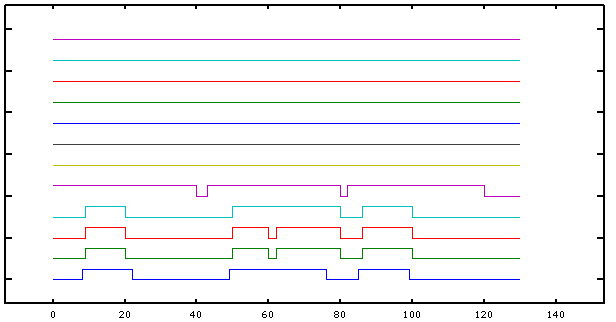
\includegraphics[width=0.9\textwidth]{./testWhiteNoise.png}
 % testWhiteNoise.png: 616x322 pixel, 72dpi, 21.73x11.36 cm, bb=0 0 616 322
\end{figure}
% \subsection{Caso di test di tolleranza al rumore bianco}
% Il protagonista di questo caso di test \`e il file Normal vesicular.wav che contiene un suono respiratorio normale disturbato da un rumore leggero. A questo file aggiungiamo con Audacity del rumore bianco di intensit\`a crescente e valutiamo le prestazioni del sistema. Il file ha le seguenti caratteristiche:
% \begin{itemize}
%  \item 
%     L'intensit\`a massima \`e circa $0.2dB$.
%   \item
%     L'intensit\`a media delle fasi inspiratorie \`e circa $0.08dB$.
%   \item
%     L'intensit\`a media delle fasi di pause respiratorie \`e circa $0.02dB$.
% \end{itemize}
% 
% L'intensit\`a del rumore aggiunto va da $0dB$ a $0.2dB$ con un incremento di $0.02dB$, quindi eseguiamo $11$ test. 
% In nessun caso era presente una apnea troppo lunga e in nessun caso l'algoritmo ha rilevato la presenza di una apnea troppo lunga quindi dal punto di vista del riconoscimento di apnee troppo lunghe, l'algoritmo funziona in modo corretto. 
% \`E comunque interessante valutare l'output dell'algoritmo con un maggior livello di dettaglio. 
% La figura \ref{testNormalWhiteNoise} illustra una rappresentazione dell'output dell'algoritmo sui file di test e contiene un grafico per ogni file di input.
% \begin{figure}
%  \centering
%  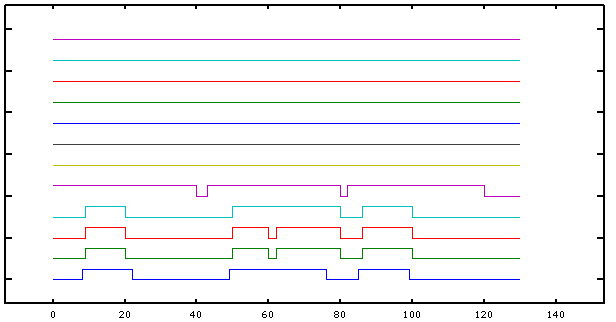
\includegraphics[width=0.9\textwidth]{./testWhiteNoise.png}
%  % testWhiteNoise.png: 1366x768 pixel, 72dpi, 48.19x27.09 cm, bb=0 0 1366 768
%   \caption{Risultati del test di tolleranza al rumore bianco.}
%   \label{testNormalWhiteNoise}
% \end{figure}
% 
% I valori sulle ascisse segnano il tempo in decimi di secondo.
% I grafici contenuti nella figura dal basso verso l'alto escluso il primo sono relativi a file che hanno una quantit\`a di rumore crescente e mostrano quali parti dei rispettivi file vengono riconosciuti come respiro e quali parti vengono riconosciuti come apnea.
% Invece il primo grafico in basso rappresenta il file originale in termini di fasi di respiro e fasi di pausa, stimate da un ascolto del file.
% I valori di questo grafico sono approssimativi e non \`e possibile ottenere valori pi\`u precisi se non si misura il flusso d'aria in modo diretto.
% Notiamo che gli ultimi $7$ grafici dal basso sono semplicemente dei segmenti di retta, questo perch\`e l'algoritmo riconosce l'intero file come respirazione cio\`e non riconosce alcuna pausa. 
% Mentre nei primi $5$ grafici dal basso il segmento di retta pu\`o essere in basso ad indicare una pausa oppure in alto ad indicare la presenza di una inspirazione o di una espirazione.
% 
% 
% % Nel grafico in figura \ref{graficoCasoDiTestRumoreBianco}, l'asse delle ascisse riporta la quantit\`a di rumore bianco aggiunto in termini di percentuale di decibel di rumore rispetto all'intensit\`a massima del respiro, mentre l'asse delle ordinate riporta l'errore calcolato in base a quanto detto nella sottosezione \ref{valutareOutput}.

\end{frame}







\part{Conclusioni}
\chapter{Conclusioni}

  \section{Commenti ai risultati ottenuti}

    I risultati ottenuti sono incoraggianti e costituiscono solo un punto di partenza verso un sistema usabile in uno scenario reale.


  \section{Sviluppi futuri}
    L'applicazione pu\`o essere modificata per:
    \begin{itemize}
      \item
	Migliorare il riconoscimento delle fasi respiratorie.
      \item
	Aggiungere la possibilit\`a di classificare i suoni respiratori secondo la classificazione \ref{sec:Analisiacusticadeisuonirespiratori}.
      \item
	Estendere l'applicazione con la funzione di riconoscere gli schemi di respiro secondo quanto specificato nella sezione \ref{schemirespiri}
    \end{itemize}


    Si possono sviluppare alcuni pezzi mancanti dell'applicazione ad esempio:
    \begin{itemize}
      \item 
	Implementare una interfaccia con uno stetoscopio elettronico e fare dei test su soggetti affetti da sindrome di apnea del sonno.
      \item
	Implementare un algoritmo di stima del flusso respiratorio.
    \end{itemize}
  

    Un altro sviluppo futuro consiste nello studiale la portabilit\`a dell'applicazione su un dispositivo mobile, sia nel caso in cui si usa il microfono in dotazione del dispositivo che nel caso in cui il dispositivo riceva i dati da uno stetoscopio elettronico. 
    Per questo scopo una tecnologia da valutare \`e J2ME.


    Ci sono vari modi di procedere utili alla ricerca nell'ambito dell'analisi dei suoni respiratori, ad esempio:
    \begin{itemize}
      \item
	Creare un database di registrazioni di suoni respiratori.
      \item	
	Creare un database di casi di test completo secondo quanto indicato nel capitolo \ref{valutazione}. 
      \item	
	Creare un modello acustico approssimato del torace.
      \item
	Implementare dei meccanismi di tolleranza al rumore esterno. 
	Ad esempio usare due microfoni: uno che registra il rumore ambientale e uno che registra i suoni respiratori e usare il modello acustico per estrarre il rumore ambientale dai suoni respiratori.
      \item
	Fare una analisi approfondita dello stato dell'arte della separazione dei suoni cardiovascolari dai suoni respiratori, partendo ad esempio dagli articoli \cite{separazione1, separazione2, separazione3, separazione4, separazione5, separazione6}.
%       \item
% 	Fare delle ricerche su quale dovrebbe essere la soglia di rischio
    \end{itemize}
\begin{thebibliography}{99}




% \bibitem{RusselNorvig}
%   Stuart Russel, Peter Norvig,
%   \emph{Artificial intelligence, },
%   .


% \bibitem{russel}
%   Stuart Russell, Peter Norvig,
%   \emph{Artificial Intelligence: A Modern Approach, 3rd ed.},
%   Prentice Hall, 2010.

% \bibitem{UrviPatel}
%   Urvi Patel,
%   \emph{Computerized respiratory sound analysis: an exploration of methods},
%   CWRU School of Engineering, Department of Physics, 2011.

% \bibitem{LauraMason}
%   Laura Mason,
%   \emph{Signal processing methods for non invasive respiration monitoring},
%   University of Oxford, 2002,


% \bibitem{Leontios}
%   Leontios Hadjileontiadis,
%   \emph{Lung sounds: an advanced signal processing perspective},
%   Systhesis lectures on biomedical engineering, 2009.

% \bibitem{SCE}
%   Sun X, Cheetham BM, Earis JE,
%   \emph{Real time analysis of lung sounds},
%   Department of Electrical Engineering \& Electronics, Liverpool University, UK.

% ____________________________________________________________________________________________________________________________________ %
% ____________________________________________________________________________________________________________________________________ %
% ____________________________________________________________________________________________________________________________________ %

\bibitem{CACMVS}
  G. Charbonneau, E. Ademovic, B.M.G. Cheetham, L.P. Malmberg, J. Vanderschoot, A.R.A. Sovij\"{a}rvi.
  \emph{Basic techniques for respiratory sound analysis}.

\bibitem{GPA}
  N. Gavriely, Y. Palti, G. Alroy.
  \emph{Spectral characteristics of normal breath sounds}.
  Journal of applied physiology  1981 Feb;50(2):307-14.

\bibitem{SKCAKM}
  S.K. Chowdhury, A.K.Majumder.
  \emph{Digital spectrum analysis of respiratory sounds}.
  IEEE Transactions on Biomedical Engineering. 
  Date of Publication: Nov. 1981. 
  Volume: BME-28, Issue: 11 
  Page(s):784-788 


\bibitem{CORS}
  Simon M\"{u}ller.
  \emph{Classification of Respiratory Sounds}.
  Institut f\"{u}r Stochastik und Anwendungen, Universitaet Stuttgart.
  \url{www.isa.uni-stuttgart.de/LstStoch/Mueller/rbk_17_12_08.pdf}.
  data di accesso 28/01/2013.
  
\bibitem{ADT}
  \url{http://atlantemedicina.wordpress.com/2008/11/04/auscultazione-del-torace/}\\
  data di accesso 28/01/2013.

\bibitem{KoronaKokar}
  Zbigniew Korona, Mieczyslaw M. Kokar.
  \emph{Lung sound recognition using model theory based feature selection and fusion}.
  Applied Signal Processing (October 1998), 5(3), pg. 152-169. 
%   Department of electrical and computer engineering,  Northeastern university 360 Huntington Avenu.
  


\bibitem{kandaswamy}
  C. Kandaswamy.
  \emph{Neural classification of lung sounds using wavelet coefficients}.
  Computer in biology and medicine,  Volume 34, Issue 6, September 2004, Pages 523 - 537.

\bibitem{DOIAERSINTSOTHT}
  Kompis, M. 
  \emph{Distribution of inspiratory and expiratory respiratory sound intensity on the surface of the human thorax}.
  Engineering in Medicine and Biology Society, 1997. Proceedings of the 19th Annual International Conference of the IEEE.

% ____________________________________________________________________________________________________________________________________ %
% ____________________________________________________________________________________________________________________________________ %
% ____________________________________________________________________________________________________________________________________ %


\bibitem{TLSA}
  Rosqvist T, Paajanen E, Kallio K, Rajala HM, Katila T, Piiril\"{a} P, Malmberg P, Sovij\"{a}rvi A.
  \emph{Toolkit for lung sound analysis}.
  Department of Technical Physics, Helsinki University of Technology, Finland.

\bibitem{RSCUCAGMM}
  M. Bahoura, C. Pelletier.
  \emph{Respiratory sounds classification using cepstral analysis and gaussian mixture models}.
  D\'epartement de Math\'ematiques, d'Informatique et de G\'enie (DMIG).
  Universit\`e du Qu\'ebec \`e Rimouski, Rimouski, Qc, Canada, G5L 3A1

\bibitem{ADFMFPLS}
  P.A. Mastorocostas, D.N. Varsamis, C.A. Mastorocostas, C.S. Hilas.
  \emph{A Dynamic Fuzzy Model for Processing Lung Sounds}.
  Department of Informatics and Communications Technological Educational Institute of Serres 62124, Serres, Greece.

\bibitem{ANAAFIORS}
  Feng Jin, Student Member, IEEE and Farook Sattar, Member, IEEE.
  \emph{A new automaed approach for identification of respiratory sounds}.
  School of Electrical and Electronic Engineering, Nanyang Technological University, Nanyang Avenue, Singapore 639798.

\bibitem{PKW}
  Hans Pasterkamp, Steve S. Kraman, George R. Wodicka.
  \emph{Respiratory sounds: advances beyond the stethoscope}.

\bibitem{SoundRepositories}
  Sound repositories:
  \begin{itemize}
    \item 
      \url{http://solutions.3mitalia.it/wps/portal/3M/it_IT/Littmann/stethoscope/education/heart-lung-sounds/}    
    \item
      \url{http://tracheostomy.com/resources/videos/index.htm}
    \item
      \url{http://faemse.org/downloads.html}
    \item
      \url{http://www.meddean.luc.edu/lumen/MedEd/medicine/pulmonar/pd/auditory.htm}
  \end{itemize}

  

\bibitem{AntoniettaBisulli}
  Antonietta Bisulli.
  \emph{Sindrome delle apnee ostruttive nel sonno(osas): effetti cognitivi del trattamento con pressione continua positiva(CPAP)}.
  Dottorato di ricerca. Universit\`a di Bologna.
  
\bibitem{NHLBI}
  NHLBI: Health Information for the Public. 
  \emph{Sleep Apnea: What Is Sleep Apnea?}.
  U.S. Department of Health and Human Services. 

\bibitem{OSARFSD}
  H. Klar Yaggi, M.D., M.P.H., John Concato, M.D., M.P.H., Walter N. Kernan,
  M.D., Judith H. Lichtman, Ph.D., M.P.H., Lawrence M. Brass, M.D., and Vahid Mohsenin, M.D.
  \emph{Obstructive Sleep Apnea as a Risk Factor for Stroke and Death}.
  New England Journal of Medicine 2005; 353:2034-2041N.

\bibitem{DNPSDOSA}
  Apoor S. Gami, M.D., Daniel E. Howard, B.S., Eric J. Olson, M.D., and Virend K. Somers, M.D., Ph.D.
  \emph{Day Night Pattern of Sudden Death in Obstructive Sleep Apnea}.
  New England Journal of Medicine 2005; 352:1206-1214.

\bibitem{PCHDIIRE}
  Christopher Wren, Sam Richmond, Liam Donaldson.
  \emph{Presentation of congenital heart disease in infancy: implications for routine examination}.
  Archive of Disease in Childhood; Fetal and Neonatal Ed. 1999 January; 80(1): F49–F53.

% \bibitem{Forgacs}
%   \emph{Functional Basis of Pulmonary Sounds}
%   Paul Porgacs,
%   journal.publications.chestnet.org

% ____________________________________________________________________________________________________________________________________ %
\bibitem{Pekonen}
  Jussi Pekonen.
  \emph{Onset detection methods for musical sounds}.
  Helsinki university of technology.

\bibitem{Bello}
  Juan Pablo Bello, Laurent Daudet, Samer Abdallah, Chris Duxbury, Mike Davies, and Mark B. Sandler.
  \emph{A Tutorial on Onset Detection in Music Signals}.
% ____________________________________________________________________________________________________________________________________ %

\bibitem{Kauppinen}
  lsmo Kauppinen.
  \emph{Methods for detecting impulsive noise in speech and audio signals}.
  University of Turku, Department of Physics, FIN-ZOOl4 Turku, Finland.


\bibitem{anatomiaRespiratorio}
   \url{ http://pacs.unica.it/biblio/fisiopatologia/fisiopatologia1.pdf}\\
   data di accesso: 28/01/2013.


\bibitem{NSCMBKA}
  Roberto Marani, Gennaro Gelao, and Anna Gina Perri.
  \emph{A New System for Continuous Monitoring of Breathing and Kinetic Activity}.
  Electrical and Electronic Department, Polytechnic of Bari, Via E. Orabona, Bari 70125, Italy.

\bibitem{Invasivita}
  \url{http://it.wikipedia.org/wiki/Invasivit\`a}\\
  data di accesso: 28/01/2013.


\bibitem{ASDBOS}
  Arzt M, Young T, Finn L, Skatrud JB, Bradley TD.
  \emph{Association of sleep disordered breathing and the occurrence of stroke}.
  Toronto General Hospital, University Health Network, 9N 943, 200 Elizabeth Street, Toronto, ON M5G 2C4, Canada.

\bibitem{ASPODUOCSS}
  Yildirim I, Ansari R, Moussavi Z.
  \emph{Automated respiratory phase and onset detection using only chest sound signal}.
  University of Illinois at Chicago, IL 60607, USA.


\bibitem{BARFUTS}
  Saiful Huq, Azadeh Yadollahi, Zahra Moussavi.
  \emph{Breath Analysis of Respiratory Flow using Tracheal Sounds}.
  Department of Electrical and Computer Engineering, University of Manitoba, Winnipeg, MB, Canada.


%_______________________________________________________________________________________________________________________________________$

\bibitem{PneumotacofragoTreCani}
  \url{http://www.treccani.it/vocabolario/pneumotacografo/}\\
  data di acesso: 29/01/2013.
\bibitem{WikiSpirPneu}
  \url{http://it.wikipedia.org/wiki/Spirometro#Spirometro_con_pneumotacografo}\\
  data di acesso: 29/01/2013.

\bibitem{polisonnografo}
  \url{http://www.nlm.nih.gov/medlineplus/ency/article/003932.htm}\\
  data di accesso: 04/02/2013.
%_______________________________________________________________________________________________________________________________________$

\bibitem{TFC}
  Tiago H. Falk and Wai Yip Chan.
  \emph{Modulation filtering for heart and lung sound separation from breath sound recordings}.
  Department of Electrical and Computer Engineering, Queen's University, Canada.

\bibitem{ARSAPD}
  \emph{Acoustical respiratory signal analysis and phase detection}.
  S. Le Cam, Ch. Collet, F. Salzenstein.
  Universit\'e Strasbourg 1.

\bibitem{SCRSA}
  A.R.A. Sovij\"{a}rvi, J. Vanderschoot, J.E. Earis.
  \emph{Standardization of computerized respiratory sound analysis}.





%__________________________________________________________________________________$

\bibitem{RSDUVFD}
  Yee Leng Yap, Zahra Moussavi,
  \emph{Respiratory onset detection using variance fractal dimension},
  Department of Electrical Engineering, University of Manitoba.

\bibitem{FLSCTWFDA}
  January Gnitecki, Zahra Moussavi.
  \emph{The fractality of lung sounds: A comparison of three waveform fractal dimension algorithms}.
  Faculty of Engineering, Department of Electrical and Computer Engineering, University of Manitoba, Winnipeg, MB Canada R3T 5V6.

%__________________________________________________________________________________$



\bibitem{DECE}
  Joo S. Chuah , Zahra K. Moussavi.
  \emph{Automated respiratory phase detection by acoustical means}.
  Department of Electrical and Computer Engineering, University of Manitoba, Winnipeg, Manitoba, R3T 2N2, Canada.
  

\bibitem{CARPDWAM}
  Z. Moussavi, M. Leopando, H. Pasterkamp, G. Rempel.
  \emph{Computerized acoustical respiratory phase detection without airflow measurament}.
  Medical and Biological Engineering and Computing 2000, Volume 38, Issue 2, pp 198-203.


\bibitem{PDUCABS}
  H. A. Mansy, T. J. Royston, R. A. Balk, R.H. Sandier.
  \emph{Pneumothorax detection using computerised analysis of breath sounds}.
  Medical and Biological Engineering and Computing 2002, Volume 40, Issue 5, pp 526-532.


\bibitem{SPMNIRM}
  Laura Mason.
  \emph{Signal Processing Methods for Non-Invasive Respiration Monitoring}.
  Trinity College Michaelmas 2002.


\bibitem{ASTFARA}
  Gina Ann Yi.
  \emph{A Software Toolkit for Acoustic Respiratory Analysis}.
  Massachussetts institute of technology.

\bibitem{TFTAAOMA}
  Stephen Webley Hainsworth.
  \emph{Techniques for the Automated Analysis of Musical Audio}.
  Magdalene College December 2003.

\bibitem{BP}
  M J Tobin; T S Chadha; G Jenouri; S J Birch; H B Gazeroglu; M A Sackner.
  \emph{Breathing patterns. 1. Normal subjects.}.
  Chest Journal. 1983;84(2):202-205.

\bibitem{ABP}
  \url{http://www.meddean.luc.edu/lumen/MedEd/medicine/pulmonar/physio/pf11.htm}\\
  data di accesso: 01/02/2013.

\bibitem{ASAHAIS}
  Susan Redline1, Gayane Yenokyan2, Daniel J. Gottlieb3,4, Eyal Shahar5, George T. O'Connor3, Helaine E. Resnick6,7, Marie Diener-West2, Mark H. Sanders8, Philip A. Wolf3, Estella M. Geraghty9, Tauqeer Ali9, Michael Lebowitz11, and Naresh M. Punjabi.
  \emph{Obstructive Sleep Apnea Hypopnea and Incident Stroke}.

\bibitem{SSAAROISITE}
  Roberto Munoz, Joaqu\'in Duran-Cantolla, Eduardo Mart\'inez-Vila, Jaime Gallego, Ram\'on Rubio, Felipe Aizpuru and Germ\'an De La Torre.
  \emph{Severe Sleep Apnea and Risk of Ischemic Stroke in the Elderly}.


% \bibitem{PCDP}
%   Ben-Ari, M.,
%   \emph{Principles of Concurrent and Distributed Programming}, 
%   Prentice Hall, 1990. 
% 
%   \bibitem{SAMHRTE} 
%     C. Liu, J. Layland, 
%     \emph{Scheduling Algorithms for Multiprogramming in a Hard Real-time Environment}, 
%    Journal of the ACM, 20(1):46--61, Jan. 1973. http://citeseer.ist.psu.edu/liu73scheduling.html

\bibitem{RealTime}
  \url{www.cis.upenn.edu/~lee/06cse480/lec-real-time-scheduling.pdf}\\
  data di accesso: 02/02/2013.
\bibitem{WikiRealTime}
  \url{http://en.wikipedia.org/wiki/Real-time}\\
  data di accesso: 02/02/2013.

\bibitem{RTDSPIA}
  S.M. Kuo, B.H. Lee, and W. Tian.
  \emph{Real-Time Digital Signal Processing: Implementations and Applications}.
  Wiley, 2006. ISBN 0-470-01495-4.


\bibitem{appaRespi}
  \url{http://it.wikipedia.org/wiki/File:Respiratory_system_complete_it.svg}\\
  data di accesso: 04/02/2013.

\bibitem{wikiMeccaRespi}
  \url{http://it.wikipedia.org/wiki/Respirazione}\\
  data di accesso: 04/02/2013.

\bibitem{meccanicaRespi}
  Ronald B. George, Richard A. Matthay, Michael A. Matthay, Richard W. Light.
  \emph{Chest Medicine: Essentials of Pulmonary and Critical Care Medicine. Edition 5}.
   Lippincott Williams and Wilkins.

% \bibitem{auscu}
%   Francesca Palma,
%   \emph{Classificazione funzionale di valvole cardiache meccaniche attraverso fonocardiografia ad ultrasuoni}
%   Tesi di laurea magistrale in bioingegneria,
%   Universit\'a degli studi di Padova,  2010/2011.




\bibitem{BBATMBS}
  \v Zilbert Tafa, Radovan Stojanovi\'c.
  \emph{Bluetooth based approach to monitoring biomedical signals}.
  Proceedings of the 5th WSEAS International Conference on Telecommunications and Informatics, Istanbul, Turkey, May 27-29, 2006 (pp415-420).


\bibitem{jstk}
  \url{http://code.google.com/p/jstk/}\\
  data di accesso: 04/02/2013.

\bibitem{clientServer}
  \url{http://en.wikipedia.org/wiki/Client-server_model}\\
  data di accesso: 04/02/2013.

\bibitem{javaSerializable}
  \url{http://docs.oracle.com/javase/1.5.0/docs/guide/serialization/spec/serial-arch.html#6428}\\
  data di accesso: 04/02/2013.

\bibitem{clustering}
  Glenn Fung.
  \emph{A Comprehensive Overview of Basic Clustering Algorithms}.
  June 22, 2001.


\bibitem{LSAITTIOTAF}
  S.S. Kraman.
  \emph{Lung Sounds: An Introduction to the Interpretation of the Auscultatory Finding}.
  Northbrook, IL: Amer. College of Chest Physicians, 1993, audio tape.

\bibitem{PatternRecognition}
  Sergios Theodoridis, Konstantinos Koutroumbas.
  \emph{Pattern recognition}.
  Elsevier Academic Press.

\bibitem{envelope}
  C. Richard Johnson, Jr, William A. Sethares, Andrew G. Klein.
  \emph{Software Receiver Design: Build Your Own Digital Communication System in Five Easy Steps}.
  Cambridge University Press. p. 417.

\bibitem{envelopeImg}
  \url{http://en.wikipedia.org/wiki/File:Signal_envelopes.png}\\
  data di accesso: 04/02/2013.

\bibitem{filtri}
  Belle A. Shenoi.
  \emph{Introduction to digital signal processing and filter design}.
  John Wiley and Sons.

\bibitem{intrrr}
  \emph{A Neural Network System for Detection of Obstructive Sleep Apnea Through SpO2 Signal Features}

\bibitem{markovtriple}
  \emph{Cha\v ines de Markov Triplet}.
  Wojciech Pieczynski.

\bibitem{markovtriple2}
  \emph{Multisensor triplet Markov chains and theory of evidence}.
  Wojciech Pieczynski.


\bibitem{fourier}
  Albert Boggess, Francis J. Narcowich.
  \emph{A first course in wavelets with Fourier analysis}.
  
\bibitem{fourier2}
  Paolo Marcellini, Carlo Sbordone.
  \emph{Analisi matematica uno}.

\bibitem{fourier3}
  \url{http://it.wikipedia.org/wiki/Fourier-Transformation}.


\bibitem{wavelet1}
  Rami Cohen.
  \emph{Signal Denoising Using Wavelets}.
  Department of Electrical Engineering Technion, Israel Institute of Technology.


\bibitem{wavelet2}
  R.J.E. Merry.
  \emph{Wavelet Theory and Applications. A literature study}.
   
\bibitem{DomTF}
  Analisi dei segnali campionati.
  \url{www.diee.unica.it/misure/Dispense/Misure_Elettroniche_dm270/Analisi_di_segnali_campionati.pdf}.
  data di accesso: 04/02/2013.

\bibitem{EAP}
  Carlo Drioli, Nicola Orio,
  \emph{Elementi di Acustica e Psicoacustica}


\bibitem{elabA}
  Corso di elaborazione audio.
  \url{http://www.mediasystemnet.it/videocorsi.html}.
  data di accesso: 04/02/2013.


\bibitem{IONDASON}
  \url{http://editoria.wiki-site.com/index.php/DIGITALIZZAZIONE}.
  data di accesso: 04/02/2013.

\bibitem{IDOMTF}
  \url{http://fisicaondemusica.unimore.it/Teorema_di_Fourier.html}.
  data di accesso: 04/02/2013.


\bibitem{SELET}
  \url {http://www.suonoelettronico.com}.
  data di accesso: 04/02/2013.

\bibitem{fusello}
  \emph{Gli stetoscopi elettronici}.  
  Giorgio Carlo Monti, Massimo Fusello.
  \url{http://www.simg.it/Documenti/Rivista/2002/08-10_2002/12.pdf}.
  data di accesso: 04/02/2013.

\bibitem{Swing}
  \url{http://docs.oracle.com/javase/6/docs/technotes/guides/swing/}.
  data di accesso: 04/02/2013.

\bibitem{jmathplot}
  \url{http://code.google.com/p/jmathplot/}.
  data di accesso: 04/02/2013.

\bibitem{audacity}
  \url{http://audacity.sourceforge.net/}
  data di accesso: 04/02/2013.


\bibitem{separazione1}
  \emph{Blind source extraction of heart sound signals from lung soud recordings exploiting periodicity of the heart sound}.
  T. Tsalaile, S. M. Naqvi, K. Nazarpour, S. Sanei and J. A. Chambers.

\bibitem{separazione2}
  \emph{Heart sounds separation from lung sounds using independent component analysis}.
  M. T. Pourazad, Z. Moussavi, F. Farahmand, R. K. Ward.
  Proceedings of the 2005 IEEE Engineering in Medicine and Biology 27th Annual Conference Shanghai, China, September 1-4, 2005.


\bibitem{separazione3}
  \emph{Modulation filtering for heart and lung sound separation from breath sound recordings}.
  Tiago H. Falk and Wai-Yip Chan.
  International Journal of Computer and Electrical Engineering, Vol. 2, No. 3, June, 2010 1793-8163.


\bibitem{separazione4}
  \emph{Separating Heart Sound from Lung Sound Using LabVIEW}
  T E Ayoob Khan, P Vijayakumar.


\bibitem{separazione5}
  \emph{Separating Heart Sounds from Lung Sounds}
  January Gnitecki, Zahara M. K. Moussavi.



\bibitem{separazione6}
  \emph{Separation of heart sound signal from lung sound signal by adaptive line enhancement}
  Thato Tsalaile, Saeid Sanei.
  15th European Signal Processing Conference (EUSIPCO 2007), Poznan, Poland, September 3-7, 2007, copyright by EURASIP.






\end{thebibliography}




% \bibliographystyle{plain}
% \bibliography{theBib}

\end{document}
